\RequirePackage{ifpdf}
\documentclass[titlesmallcaps,%
               examinerscopy,%
               copyrightpage]{uqthesis}

\newcommand{\mcomment}[1]{\reversemarginpar\marginpar{\textcolor{red}{\bf #1}}}
\newcommand\mnote[1]{\textcolor{cyan}{#1}}


%%%%% Some helpful general definitions
% Copyright (C) 2004 Paul Cochrane
%
% This program is free software; you can redistribute it and/or
% modify it under the terms of the GNU General Public License
% as published by the Free Software Foundation; either version 2
% of the License, or (at your option) any later version.
%
% This program is distributed in the hope that it will be useful,
% but WITHOUT ANY WARRANTY; without even the implied warranty of
% MERCHANTABILITY or FITNESS FOR A PARTICULAR PURPOSE.  See the
% GNU General Public License for more details.
%
% You should have received a copy of the GNU General Public License
% along with this program; if not, write to the Free Software
% Foundation, Inc., 59 Temple Place - Suite 330, Boston, MA  02111-1307, USA.

\newcommand {\tbf}[1] {\textbf{#1}}
\newcommand {\tit}[1] {\textit{#1}}
\newcommand {\tmd}[1] {\textmd{#1}}
\newcommand {\trm}[1] {\textrm{#1}}
\newcommand {\tsc}[1] {\textsc{#1}}
\newcommand {\tsf}[1] {\textsf{#1}}
\newcommand {\tsl}[1] {\textsl{#1}}
\newcommand {\ttt}[1] {\texttt{#1}}
\newcommand {\tup}[1] {\textup{#1}}

\newcommand {\mbf}[1] {\mathbf{#1}}
\newcommand {\mmd}[1] {\mathmd{#1}}
\newcommand {\mrm}[1] {\mathrm{#1}}
\newcommand {\msc}[1] {\mathsc{#1}}
\newcommand {\msf}[1] {\mathsf{#1}}
\newcommand {\msl}[1] {\mathsl{#1}}
\newcommand {\mtt}[1] {\mathtt{#1}}
\newcommand {\mup}[1] {\mathup{#1}}

%My thesis abbr.
\newcommand{\npscarf}{$\mathtt{npScarf}$}
\newcommand{\npscarfg}{$\mathtt{npScarf\_wag}$}
\newcommand{\npreader}{$\mathtt{npReader}$}
\newcommand{\npanalysis}{$\mathtt{npAnalysis}$}
\newcommand{\npbarcode}{$\mathtt{npBarcode}$}
\newcommand{\npgraph}{$\mathtt{npGraph}$}
\newcommand{\canu}{$\mathtt{Canu}$}
\newcommand{\unicycler}{$\mathtt{Unicycler}$}
\newcommand{\spades}{$\mathtt{SPAdes}$}
\newcommand{\albacore}{$\mathtt{Albacore}$}
\newcommand{\racon}{$\mathtt{Racon}$}
\newcommand{\metrichor}{$\mathtt{Metrichor}$}
\newcommand{\minimap}{$\mathtt{minimap2}$}
\newcommand{\miniasm}{$\mathtt{miniasm}$}
\newcommand{\bwa}{$\mathtt{BWA\text{-}MEM}$}

\newcommand{\ec}{\emph{E.~coli}}
\newcommand{\sce}{\emph{S.~cerevisae}}
\newcommand{\kp}{\emph{K.~pneumoniae}} 

\newcommand{\IE}{\emph{i.e.}}
\newcommand{\EG}{\emph{e.g.}}
\newcommand{\review}[1]{\textcolor{red}{#1}}

\newcommand {\figwidth} {100mm}
\newcommand {\Ref}[1] {Reference~\cite{#1}}
\newcommand {\Sec}[1] {Section~\ref{#1}}
\newcommand {\App}[1] {Appendix~\ref{#1}}
\newcommand {\Chap}[1] {Chapter~\ref{#1}}
\newcommand {\etal} {\emph{~et~al.}}
\newcommand {\bul} {$\bullet$ }   % bullet
\newcommand {\fig}[1] {Figure~\ref{#1}}   % references Figure x
\newcommand {\imp} {$\Rightarrow$}   % implication symbol (default)
\newcommand {\impt} {$\Rightarrow$}   % implication symbol (text mode)
\newcommand {\impm} {\Rightarrow}   % implication symbol (math mode)
\newcommand {\vect}[1] {\mathbf{#1}}
\newcommand {\hvect}[1] {\hat{\mathbf{#1}}}
\newcommand {\del} {\partial}
\newcommand {\eqn}[1] {Equation~(\ref{#1})}
\newcommand {\tab}[1] {Table~\ref{#1}} % references Table x
\newcommand {\half} {\frac{1}{2}}
\newcommand {\ten}[1] {\times10^{#1}}
\newcommand {\bra}[2] {\mbox{}_{#2}\langle #1 |}
\newcommand {\ket}[2] {| #1 \rangle_{#2}}
\newcommand {\Bra}[2] {\mbox{}_{#2}\left.\left\langle #1 \right.\right|}
\newcommand {\Ket}[2] {\left.\left| #1 \right.\right\rangle_{#2}}
\newcommand {\im} {\mathrm{Im}}
\newcommand {\re} {\mathrm{Re}}
\newcommand {\braket}[4] {\mbox{}_{#3}\langle #1 | #2 \rangle_{#4}}
\newcommand {\dotprod}[4] {\mbox{}_{#3}\langle #1 | #2 \rangle_{#4}}
\newcommand {\trace}[1] {\text{tr}\left(#1\right)}

% spell things correctly
\newenvironment{centre}{\begin{center}}{\end{center}}
\newenvironment{itemise}{\begin{itemize}}{\end{itemize}}

\usepackage{epigraph}
\setlength\epigraphwidth{.5\textwidth}
\setlength\epigraphrule{0pt}

\usepackage{pdfpages} 

\usepackage{acronym} 
\usepackage[titletoc]{appendix}
\usepackage{mathtools}
\usepackage{play}
\usepackage[grey,times]{quotchap}
\usepackage{makeidx}
\usepackage{xcolor,colortbl}
\usepackage{longtable}
\usepackage{booktabs}
\usepackage{hyperref}
\usepackage{pdflscape}
\usepackage{afterpage}
%%%%% set up the bibliography style
\bibliographystyle{uqthesis}  % uqthesis bibliography style file, made
			      % with makebst

%%%%% optional packages
\usepackage[square,comma,numbers,sort&compress]{natbib}
		% this is the natural sciences bibliography citation
		% style package.  The options here give citations in
		% the text as numbers in square brackets, separated by
		% commas, citations sorted and consecutive citations
		% compressed
		% output example: [1,4,12-15]

\usepackage[nottoc]{tocbibind}
				% allows the table of contents, bibliography
				% and index to be added to the table of
				% contents if desired, the option used
				% here specifies that the table of
				% contents is not to be added.
				% tocbibind needs to be after natbib
				% otherwise bits of it get trampled.

\usepackage{amsmath,amsfonts,amssymb} % this is handy for mathematicians and physicists
			      % see http://www.ams.org/tex/amslatex.html

% \usepackage{showkeys} % this shows what labels you are using for cross
		      % references

\usepackage{graphicx} % standard graphics package for inclusion of
		      % images and eps files into LaTeX document

\usepackage{multirow} 

% For pseudocode
\usepackage[linesnumbered,boxed,ruled,vlined]{algorithm2e}
\newcommand\mycommfont[1]{\footnotesize\ttfamily\textcolor{blue}{#1}}
\SetCommentSty{mycommfont}
% For code embedding (Bash, Java...)
\usepackage{listings}
\lstset{basicstyle=\ttfamily,
  showstringspaces=false,
  commentstyle=\color{red},
  keywordstyle=\color{blue}
}

\usepackage{tocloft}

\usepackage{float}
\usepackage[caption = false]{subfig}
% this code hacked from that of R Chandrasekhar from UWA
\newif\ifpdf
\ifx\pdfoutput\undefined
	\pdffalse    % we are not running pdfLaTeX
\else
	\pdfoutput=1 % we are running pdfLaTeX
	\pdftrue
\fi

\ifpdf
	\DeclareGraphicsExtensions{.pdf}  % this command defined in graphicx
	\pdfcompresslevel=9  % 0: no compression, 9: highest compression
			     % or, set compress_level 9 in file pdftex.cfg
\else
	\DeclareGraphicsExtensions{.ps}
\fi

% put in an index?
% \makeindex

%set numbering for subsubsection
\setcounter{secnumdepth}{3}

\begin{document}

\frontmatter

%%%%% Acknowledgements, titlepage, abstract, list of publications
\title{
Real-time analysis for Nanopore sequencing data}
\author{Son Hoang Nguyen}

\department{Institute for Molecular Bioscience}  % institute/department

% honours students will want to override the \degreetext variable with
% something appropriate like that here:
%\renewcommand{\degreetext}%

\titlepage
\chapter*{Abstract}
% Third generation sequencing technologies such as the Oxford Nanopore Technologies has been widely considered to be a turning point due to its ability to decode much longer reads in a real-time fashion. This has potential to enable scaffold and finish assemblies in real-time while the sequencing process is still in progress. 
%\mcomment{I think you should not limited to ONT,}
The introduction of third-generation sequencing technologies presents many challenges to the traditional methods in which bioinformatics is applied to genomics data. The MinION thumb-drive sequencing device has gained great attention from researchers worldwide. Despite the relatively high error rates compared to Second Generation Sequencing technologies, the nanopore approach is widely considered to be a turning point due to its ability to decode much longer reads (tens or even hundreds of kilobase pairs) in a real-time fashion.

Prior to the work presented in this thesis, there was no available method that could scaffold and finish assemblies in real-time while the nanopore sequencing run is still in progress. Such a method is desirable because it offers the opportunity to obtain analysis results as soon as sufficient data are generated.
With real-time analysis, answers to questions of interests
could be obtained \emph{in situ}, in an automated manner that saves considerable amount of time and resources compared to the conventional approach of sending sample to a sequencing centre, waiting for bulk data, and conducting a batch analysis. 
On top of that, streaming analysis can help to avoid under- and over-sequencing which could result in either the generation of more sequence data than required at greater cost or a low quality assembly if insufficient data are generated.

For the reasons mentioned above, the motivation of this thesis project is to develop methodologies for streaming data analysis of long reads for real-time finishing genome sequences.
As the initial result, in Chapter~\ref{ch:npscarf}, I introduce \npscarf{} which can scaffold and complete short read assemblies alongside with the long read sequencing run. This tool operates on an input of contigs, attempting to bridge them together by using long-read data and reports assembly metrics in real-time so the sequencing run can be terminated once an assembly of sufficient quality is obtained.

It is also desirable to extend the pipeline application for multiple samples at the same time, through a parallel mechanism known as barcoded sequencing.
In Chapter~\ref{ch:npbarcode}, \npbarcode{}, a tool supporting real-time demultiplexing of nanopore sequencing data, is employed to serve that purpose. 
Depending on requirements, users can choose to run the dedicated demultiplexer from the command line or using it as part of the $\mathtt{npReader}$'s graphical user interface (GUI). The tool provides practitioners a flexible option to monitor a barcoded sequencing run as well as to integrate pooled sequencing into a streaming analysis pipeline. For example, in combination with \npscarf{}, we can complete multiple genomes in parallel.

Users can also provide underlying assembly graph structure from short-read assemblers for better quality. This approach is described in Chapter~\ref{ch:npgraph}. In which, a streaming algorithm is implemented together with GUI in \npgraph{}. The benefits of using assembly graph stem from the fact that by traversing the graph of the contigs' building blocks, we can reduce the number of misassemblies and errors in the final sequences. 

Chapter~\ref{ch:concatemers} discusses another application of nanopore sequencing for decoding small genomes. By employing rolling circle amplification, long reads containing multiple copies of a given viral genome can be obtained. The duplicated patterns are possibly identified by a detection module that can even work with raw signal data. The developed modules, which allow for single-molecule genome assembly of small genomes, can be integrated into a streaming pipeline for real-time analyses as well.

In summary, my thesis project aims to develop and apply in-house tools that aid genome assembly and analysis in real-time in an attempt to facilitate the applications of nanopore sequencing for various use cases, including but not limited to microbial genomics.

\cleardoublepage

\afterpage{\null\thispagestyle{empty}\newpage}

\thispagestyle{plain}
\newpage

\thispagestyle{plain}
% Declaration by author
\begin{center}
\Large \textsc{Declaration by author}
\end{center}

\vspace{0.6cm}

This thesis is composed of my original work, and contains no material previously published or written by another person except where due reference has been made in the text. I have clearly stated the contribution by others to jointly-authored works that I have included in my thesis.

\vspace{0.6cm}

I have clearly stated the contribution of others to my thesis as a whole, including statistical assistance, survey design, data analysis, significant technical procedures, professional editorial advice, financial support and any other original research work used or reported in my thesis. The content of my thesis is the result of work I have carried out since the commencement of my higher degree by research candidature and does not include a substantial part of work that has been submitted to qualify for the award of any other degree or diploma in any university or other tertiary institution. I have clearly stated which parts of my thesis, if any, have been submitted to qualify for another award.

\vspace{0.6cm}

I acknowledge that an electronic copy of my thesis must be lodged with the University Library and, subject to the policy and procedures of The University of Queensland, the thesis be made available for research and study in accordance with the Copyright Act 1968 unless a period of embargo has been approved by the Dean of the Graduate School. 

\vspace{0.6cm}

I acknowledge that copyright of all material contained in my thesis resides with the copyright holder(s) of that material. Where appropriate I have obtained copyright permission from the copyright holder to reproduce material in this thesis and have sought permission from co-authors for any jointly authored works included in the thesis.

\afterpage{\null\thispagestyle{empty}\newpage}
\newpage

\thispagestyle{plain}
\begin{center}
\Large \textsc{Publications included in this thesis}
\end{center}

Involved publications are exclusively listed below with the name(s) of candidate highlighted in \textbf{bold} and (co)first author(s) \underline{underlined}.
Reproduction and/or remake of any publication or parts of project in this thesis has been approved by its corresponding authors.

\begin{itemize}
\item \underline{Cao, M. D., \textbf{Nguyen, S. H.}}, Ganesamoorthy, D., Elliott, A. G., Cooper, M. A., and Coin, L. J. (2017). Scaffolding and completing genome assemblies in real-time with nanopore sequencing. \emph{Nature Communications}, 8, 14515. \label{pub:npscarf}
\item \underline{\textbf{Nguyen, S. H.}}, Duarte, T. P., Coin, L. J., and Cao, M. D. (2017). Real-time demultiplexing Nanopore barcoded sequencing data with npBarcode. \emph{Bioinformatics}, 33(24), 3988-3990. \label{pub:npbarcode}
\end{itemize}

\begin{center}
\Large \textsc{Submitted manuscripts included in this thesis}
\end{center}
\begin{itemize}
\item \underline{Pitt, M.}, \textbf{Nguyen, S. H.}, Duarte, T. P., Blaskovich, M., Cooper, M., and Coin, L. (2018). Evaluating the Genome and Resistome of Extensively Drug-Resistant \emph{Klebsiella pneumoniae} using Native DNA and RNA Nanopore Sequencing. Submitted to \emph{Nature Microbiology} . \label{pub:rnaseq}
% \item \underline{Bialasiewicz, S.}, Duarte, T.P., \textbf{Nguyen, S.H.}, Sukumaran, V., Stewart, A., Appleton, S., Pitt, M.E., Bainomugisa, A., Jennison, A.V., Graham, R. and Coin, L.J., (2018). Rapid Diagnosis of \emph{Capnocytophaga canimorsus} Septic Shock in an Immunocompetent Individual Using Real-Time Nanopore Sequencing. \emph{Preprints}, 2018110395 (doi: 10.20944/preprints201811.0395.v1).
\end{itemize}

\begin{center}
\Large \textsc{Other publications during candidature}
\end{center}
\paragraph*{\textit{Peer-reviewed papers:}}
\begin{itemize}
\item \underline{Jin, M.}, Lu, J., Chen, Z., \textbf{Nguyen, S.H.}, Mao, L., Li, J., Yuan, Z. and Guo, J. (2018). Antidepressant fluoxetine induces multiple antibiotics resistance in \emph{Escherichia coli} via ROS-mediated mutagenesis. \emph{Environment international}, 120, 421-430.
\item \underline{Lu, J.}, Wang, Y., Li, J., Mao, L., \textbf{Nguyen, S.H.}, Duarte, T., Coin, L., Bond, P., Yuan, Z. and Guo, J. (2018). Triclosan at environmentally relevant concentrations promotes horizontal transfer of multidrug resistance genes within and across bacterial genera. \emph{Environment international}, 121, 1217-1226.
\item \underline{Lu, J.}, Jin, M., \textbf{Nguyen, S.H.}, Mao, L., Li, J., Coin, L.J., Yuan, Z. and Guo, J. (2018). Non-antibiotic antimicrobial triclosan induces multiple antibiotic resistance through genetic mutation. \emph{Environment international}, 118, 257-265.
\end{itemize}

% \paragraph*{\textit{Preprints:}}
% \begin{itemize}
% \item \underline{Pitt, M.}, \textbf{Nguyen, S. H.}, Duarte, T. P., Blaskovich, M., Cooper, M., and Coin, L. (2018). Evaluating the Genome and Resistome of Extensively Drug-Resistant \emph{Klebsiella pneumoniae} using Native DNA and RNA Nanopore Sequencing. \emph{bioRxiv}, 482661. \label{pub:rnaseq}
% \item \underline{Bialasiewicz, S.}, Duarte, T.P., \textbf{Nguyen, S.H.}, Sukumaran, V., Stewart, A., Appleton, S., Pitt, M.E., Bainomugisa, A., Jennison, A.V., Graham, R. and Coin, L.J., (2018). Rapid Diagnosis of \emph{Capnocytophaga canimorsus} Septic Shock in an Immunocompetent Individual Using Real-Time Nanopore Sequencing. \emph{Preprints}, 2018110395 (doi: 10.20944/preprints201811.0395.v1).
% \end{itemize}

% \paragraph*{\textit{Manuscripts in preparation:}}
% \begin{itemize}
% \item \textbf{Nguyen, S. H.}, Cao, M. D., and Coin, L. J.  Resolve assembly graph in real-time with nanopore sequencing. \label{pub:npgraph}
% \item Ngo, T.H., \textbf{Nguyen, S. H.}, Duarte, T. P., Coin, L. J., and Geering, A. Evaluation of rolling circle DNA amplification in combination with nanopore sequencing for detection of caulimovirids. \label{pub:concatemer}
% \end{itemize}

\paragraph*{\textit{Conferences abstract:}}
\begin{itemize}
\item Poster: \emph{Completing microbial draft genomes with Oxford Nanopore sequencing data}.
Has been presented in:
\begin{itemize}
\item[$\bullet$] The Australian Bioinformatics And Computational Biology Society (\textbf{ABACBS}) -- Garvin Institute of Medical Research, Sydney 2015.
\item[$\bullet$] Big Biology and Bioinformatics Symposium ($\mathbf{B^3}$) -- Queensland University of Technology, Brisbane 2015.
\end{itemize}
\item Oral presentation: \emph{Scaffolding and completing genome assemblies in real-time with nanopore sequencing.} \textbf{COMBINE} Symposium -- Queensland University of Technology, Brisbane 2016. 
\end{itemize}

\paragraph*{\textit{Web resources:}}
\begin{itemize}
\item Software presented in Chapter~\ref{ch:npscarf} and Chapter~\ref{ch:npbarcode} are bundled in Japsa (Java Package for Sequence Analysis) project \url{https://github.com/mdcao/japsa}.
\item Software presented in Chapter~\ref{ch:npgraph} and Chapter~\ref{ch:concatemers} can be found in \url{https://github.com/hsnguyen/assembly}.
\end{itemize}

% Contributions by others to the thesis
\begin{center}
\Large \textsc{Contributions by others to the thesis}
\end{center}

Dr Miranda Pitt and Tania Duarte provided details for lab experiments in Chapter~\ref{ch:npbarcode} (sample details, library preparation, sequencing methods). A/Prof Lachlan Coin, Dr Minh Duc Cao, Dr Hoang Nguyen gave feedback and revisions for the thesis.

\vspace{2cm}

\thispagestyle{plain}
% Statement of parts of the thesis submitted to qualify for the award of another degree
\begin{center}
\Large \textsc{Statement of parts of the thesis submitted to qualify for the award of another degree}
\end{center}

No works submitted towards another degree have been included in this thesis.

\vspace{2cm}

% Research Involving Human or Animal Subjects
\begin{center}
\Large \textsc{Research Involving Human or Animal Subjects}
\end{center}

No animal or human subjects were involved in this research.

\afterpage{\null\thispagestyle{empty}\newpage}
\newpage



% Acknowledgements
\thispagestyle{plain}

\begin{center}
\Large \textsc{Acknowledgements}
\end{center}

Thanks Lachlan, Minh, Lutz.

Thanks Scott Beatson, Cheong-Xin Chan, Joselph Powell.

\vspace{.3cm}

I thank Amanda Carozzi.

\vspace{.3cm}

Thanks Devika, Miranda, Tania; also Arnold, Chenxi and other Coin group members.

Thanks collaborators.

\vspace{.3cm}

Thank family.

\vspace{.3cm}

Thank world!

Tack tack tack tack tack tack tack tack tack tack tack tack tack tack tack tack tack tack
%I would like to express my greatest appreciations to my parents for their unconditional loves, trusts and faith. I would not be who I am today without their selfless contribution.   

\afterpage{\null\thispagestyle{empty}\newpage}
\newpage


% Financial support
\thispagestyle{plain}

\begin{center}
\Large \textsc{Financial support}
\end{center}

This research was supported by the University of Queensland Centennial Scholarship.

\vspace{2cm}
% Keywords
\begin{center}
\Large \textsc{Keywords}
\end{center}

bioinformatics, computational biology, genomics, antibiotic resistance, nanopore sequencing, genome assembly, real-time analysis

\vspace{2cm}
% Standard Research Classifications
\begin{center}
\Large \textsc{Australian and New Zealand Standard Research Classifications (ANZSRC)}
\end{center}

ANZSRC code: 080301, Bioinformatics software, 40\%

ANZSRC code: 060408, Genomics, 40\%

ANZSRC code: 060503, Microbial Genetics, 20\%
\vspace{2cm}

% Fields of Research (FoR) Classification
\begin{center}
\Large \textsc{Fields of Research (FoR) Classification}
\end{center}

FoR code: 0803, Computer Software, 40\%

FoR code: 0604, Genetics, 40\%

FoR code: 0605, Microbiology, 20\%
\afterpage{\null\thispagestyle{empty}\newpage}
\newpage

% Dedications
\thispagestyle{plain}

\begin{center}
\Large \textsc{Dedications}
\end{center}
This thesis is dedicated to 

\afterpage{\null\thispagestyle{empty}\newpage}
\cleardoublepage
\tableofcontents
\cleardoublepage
\listoffigures
\cleardoublepage
\listoftables
\cleardoublepage
\chapter{List of Abbreviations}

\begin{acronym}[XXXXXX] % Give the longest label here so that the list is nicely aligned
\itemsep-5pt
\acro{ACF}{Auto-correlation Function} 
\acro{AMR}{Antimicrobial Resistance} 
\acro{DNA}{Deoxyribonucleic Acid} 
\acro{DFS}{Depth First Search}
\acro{FFT}{Fast Fourier Transform}
\acro{NGS}{Next-Generation ($2^{nd}$-Gen) Sequencing}
\acro{NKDF}{Normalized Kronecker Delta Function}
\acro{NSDF}{Normalized Square Difference Function}
\acro{ONT}{Oxford Nanopore Technologies}
\acro{PacBio}{Pacific Biosciences}
\acro{PCR}{Polymerase Chain Reaction}
\acro{PDR}{Pan-Drug Resistant}
\acro{RNA}{Ribonucleic Acid}
\acro{XDR}{Extensively Drug Resistant}
\end{acronym}


\mainmatter

%%%%% Introduction
\cleardoublepage
\chapter{Introduction}\label{ch:intro}
\thispagestyle{empty}
\vspace*{\fill}
\epigraph{\emph{Genes are like the story, and DNA is the language that the story is written in}}
{--Sam Kean}

\clearpage
%%%%%%%%%%%%%%%%%%%%%%%%%%%%%%%%%%%%%%%%%%%%%%%%%%%%%%%%%%%%%%%%%%%%%%%%%%%%%%%%%%%%%
%%%%%%%%%%%%%%%%%%%%%%%%%%%%%%%%%%%%%%%%%%%%%%%%%%%%%%%%%%%%%%%%%%%%%%%%%%%%%%%%%%%%%
%%%%%%%%%%%%%%%%%%%%%%%%%%%%%%%%%%%%%%%%%%%%%%%%%%%%%%%%%%%%%%%%%%%%%%%%%%%%%%%%%%%%%
\section{Reading genome -- the book of life}
% * <hoangnguyen177@gmail.com> 2018-11-25T23:35:15.645Z:
% 
% maybe a grand-er opening ? 
% Like one of the greatest breakthrough in life science in 20th century is the ...
% history of genetic & central dogma?
The mission of decoding the genetic information of all organisms has been attracting great attention and effort from the research community over the past three decades. 
Although genomes are thought to contain nearly all the information necessary to create an organism, sequencing a genome is only the very first step towards understanding the development of an organism. 
Subsequent to genome sequencing and annotation there remains a huge amount of additional work to interpret the genome and understand how genes interact in pathways in a variety of contexts to sustain life. 
Nevertheless, the importance of the initial reading is indisputable as it would shape the details and output of any further analysis.
In fact, the competition of modern sequencing technologies have never been on hiatus, resulting in remarkably achievements in terms of both quality and quantity. 
However, unfortunately, we are still far away from having a flawless sequencer to date.

All genetic material of an organism is embraced in the term \emph{genome} mentioned earlier. Basically, the genome includes deoxyribonucleic acid (DNA) molecules -- the double helix polymers \cite{Watson1953} that virtually define a whole individual life form (except some viruses made by ribonucleic acid or RNA). 
A DNA molecule is a sequence of nucleotides, which is represented by 4 bases: adenine (A), cytosine (C), guanine (G), or thymine (T). The process of calling each and every single base of this sequence is known as \emph{DNA sequencing}. Sequencing an entire organism's genome is termed Whole Genome Sequencing (WGS). 
Innovation in sequencing technology has enabled WGS for a large variety of species with increasing genome sizes and complexity  over time, such as \emph{Haemophilus influenzae} bacterium \cite{Fleischmann1995}, \emph{Saccharomyces cerevisiae} \cite{Goffeau1996}, \emph{Caenorhabditis elegans} \cite{Sequencing1998} and \emph{Mus musculus} (mouse) \cite{Chinwalla2002}. Ultimately, the completion of the Human Genome Project \cite*{International2004} marked the beginning of the genomics era in which rapidly developing technology would make WGS much more efficient and affordable.
The cost of sequencing has been dropped drastically over time to the point that scientists are now planning for the Earth BioGenome Project, which plans to sequence 1.5 million different species across multiple continents\cite{Lewin2018earth}.

%%%%%%%%%%%%%%%%%%%%%%%%%%%%%%%%%%%%%%%%%%%%%%%%%%%%%%%%%%%%%%%%%%%%%%%%%%%%%%%%%%%%%
%%%%%%%%%%%%%%%%%%%%%%%%%%%%%%%%%%%%%%%%%%%%%%%%%%%%%%%%%%%%%%%%%%%%%%%%%%%%%%%%%%%%%
\subsection{DNA sequencing technology}

\begin{figure}[ht!]
\centering
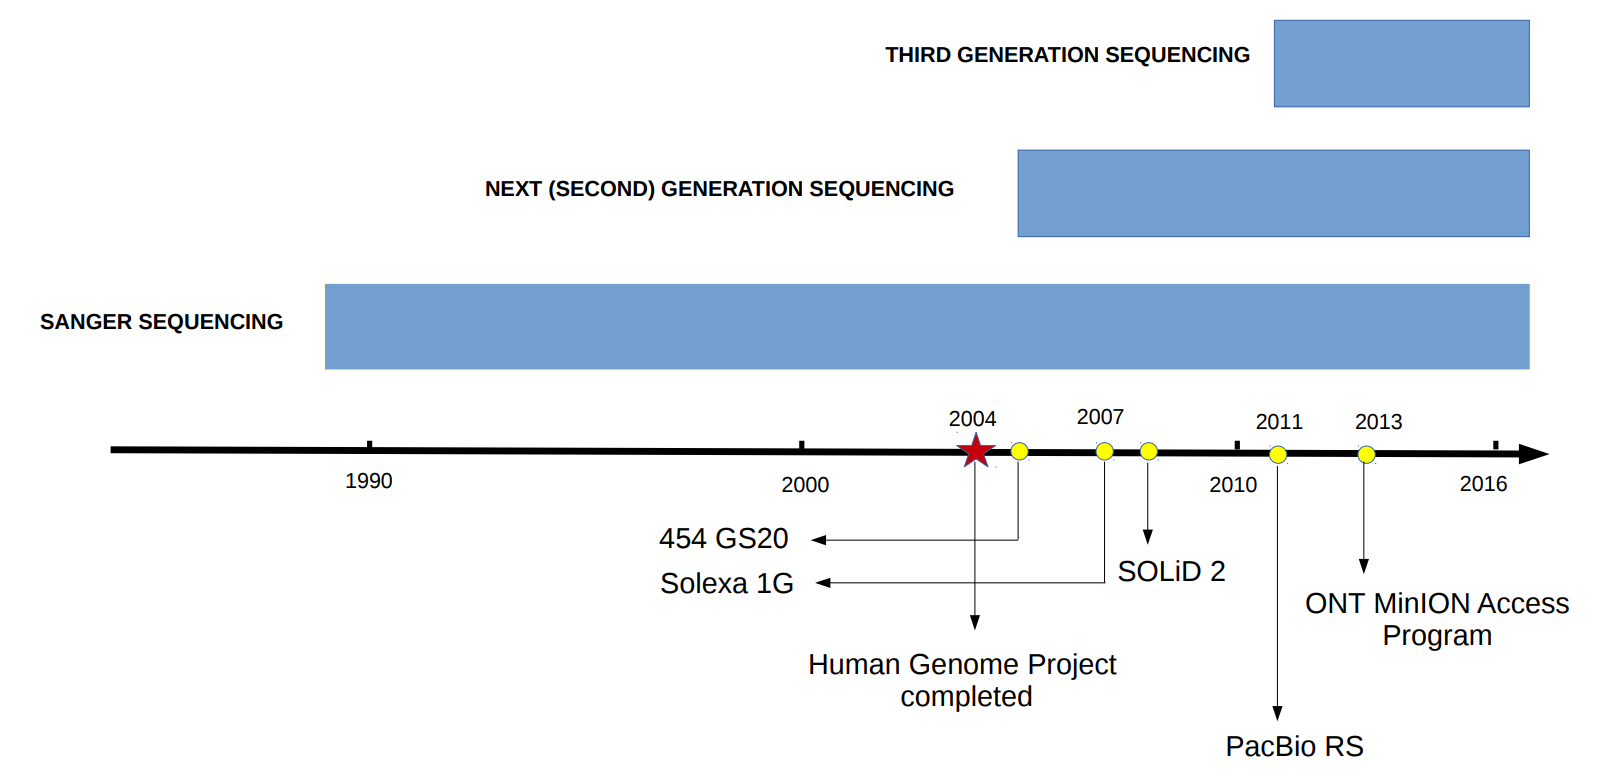
\includegraphics[width=.9\textwidth]{images/timeline.png}
\caption{Prominent sequencing platforms in the era of genomics.}
\label{Fig:nanopore}
\end{figure}
The first practical sequencing technology was invented by Frederick Sanger and colleagues \cite{Sanger1977} and as the consequence, had been named after its founder. 
Sanger sequencing, can be considered as the \emph{First generation sequencing}, employs the mechanism of selectively terminating the chain elongation by dideoxy nucleotide, which is a nucleotide analogue which lacks a 3`-hydroxyl group needed for the next incoporation and extension.
Improved Sanger platforms nowadays can output reads up to around $1$Kbp with high accuracy (99.9\%) but the yields and cost are still unreasonable compared with other methods.
In fact, Sanger sequencing contributed vastly at the beginning of the sequencing era but became supplanted later by \emph{Second-Generation Sequencing} (SGS) machines (previously known as Next-Generagetion Sequencing) which are of much larger scale and higher throughput in term of data acquired. For that reason, it is restricted in use today, and used largely only for validation or in combination with other deep-sequencing methods \cite{Freeman2009}.
SGS platforms, on the other hand, can output a large amount of DNA sequence with length up to $1$Kbp in form of single, mate-paired or paired-end reads on demand, for a large ranges of studies.
Prominent sequencing technologies include pyrosequencing \cite{Ronaghi1996,Ronaghi1998} 
(Roche 454), ion torrent(ThermoFisher), SOLiD sequencing (Applied Biosystems) and sequencing by synthesis (Illumina/Solexa).

\begin{table}[ht!]
\centering
\caption[Comparison of DNA sequencing methods in general]{Comparison of DNA sequencing methods in general. Each method may have several platforms with varied configurations for different usage. More details in \cite{Lee2013common,Mardis2017dna}.} 
\label{tab:sequencing}
\begin{tabular}{llcccc}
\hline
\toprule
\multirow{2}{*}{\textbf{Gen.}} & \multirow{2}{*}{\textbf{Sequencing methods}}& \textbf{Read length} & \textbf{Accuracy} & \textbf{Reads}  & \textbf{Time} \\
& & \textbf{(bp)} & \textbf{(\%)} & \textbf{per run} & \textbf{per run} \\ 
\hline
\rowcolor{Gray}
 \cellcolor{white} & Chain termination &  &  &  & \\
\rowcolor{Gray}
 \cellcolor{white} \multirow{-2}{*}{$1^{st}$} & (Sanger sequencing) &\multirow{-2}{*}{$400-900$} & \multirow{-2}{*}{$99.9$} & \multirow{-2}{*}{N/A} & \multirow{-2}{*}{$0.3-3$ hours} \\
\hline
 & Pyrosequencing (454) & $700$ & $99.9$ & $1$ million & $24$ hours\\
\rowcolor{Gray}
 \cellcolor{white} & Sequencing by synthesis &  &  & up to & \\
\rowcolor{Gray}
 \cellcolor{white} & (Illumina/Solexa) & \multirow{-2}{*}{up to $300$} & \multirow{-2}{*}{$>99$} &  $3$ billions & \multirow{-2}{*}{$<1-14$ days}\\
& Sequencing by ligation & \multirow{2}{*}{$75+35$} & \multirow{2}{*}{99.9} & up to & \multirow{2}{*}{$1-2$ weeks} \\
& (SOLiD sequencing) & & & $2.8$ billions & \\
\rowcolor{Gray}
 \cellcolor{white} \multirow{-6}{*}{$2^{nd}$} & Ion semiconductor & $200$ & $98$ & $5$ millions & $2$ hours\\
\hline
 & Single molecule,  & $3000$ & \multirow{2}{*}{$85$} & \multirow{2}{*}{$\approx 50$K} & \multirow{2}{*}{$2$ hours} \\
 & real-time sequencing &  on average & & & \\
\rowcolor{Gray}
 \cellcolor{white} &  & extremely &  & $\approx 150$K & $<48$ hours\\
\rowcolor{Gray}
 \cellcolor{white}\multirow{-3}{*}{$3^{rd}$} & \multirow{-2}{*}{Nanopore sequencing} & long & \multirow{-2}{*}{$85-96$} & per flow cell & (real-time output) \\
\hline
\end{tabular}
\end{table}  

After years of innovation, Illumina is currently leading the sequencing market. This giant company reportedly has much larger revenues compared to other competitors~\cite{Philippidis2018top}
%estimated as \$$2.752$ billions in 2017 
and its equipment is ubiquitous amongst genomics labs worldwide. 
In fact, the sequencing productivity, quality and deployment cost-effectiveness have been enhanced significantly with the introduction of new platforms such as MiniSeq, MiSeq series, NextSeq, HiSeq and HiSeq X and Novaseq series. These sequencers provide high-fidelity paired-end reads of length 100-300bp each.  In consequence, bacterial DNA sequencing is typically done at average sequencing depth of more than 100-folds.
In other words, each of every bases in the whole genome would be covered by around 100 reads using such platforms.
In this thesis, data from Illumina MiSeq or HiSeq were used as input for the assembly algorithms. 

The race for better sequencing technology is still going on rapidly and intensively, illustrated by the emergence of so-called \emph{Third generation} or long-read sequencing technology \cite{Munroe2010third,Bleidorn2016third} with two major reprentatives \IE{} Pacific Biosciences of California, Inc. (PacBio) and Oxford Nanopore Technologies Limited (ONT). 
As indicated by the name, the defining feature of this category is the ability to measure in real-time the signals of every single molecule and output significantly longer reads than the previous generation sequencers. 
Table \ref{tab:sequencing} presents the performances of above-mentioned sequencing platforms in term of read length, yield, accuracy and running time.

At the time this thesis being written, Illumina has come to an agreement to acquire PacBio for approximately \$$1.2$ billions in an attempt to expand its DNA sequencing capacity. At the same time,  ONT is continuing to grow into a essential player in the field of genome sequencing with remarkable success stories.
The next section will briefly shed light into TGS focusing on the latter technology.

%%%%%%%%%%%%%%%%%%%%%%%%%%%%%%%%%%%%%%%%%%%%%%%%%%%%%%%%%%%%%%%%%%%%%%%%%%%%%%%%%%%%%
\subsection{Third-generation sequencing technology}
\paragraph{Single molecule, real-time (SMRT) sequencing}
The first long-read sequencer available on market was the PacBio RS from Pacific Biosciences of California, Inc. in 2011. 

\begin{figure}[ht!]
\centering
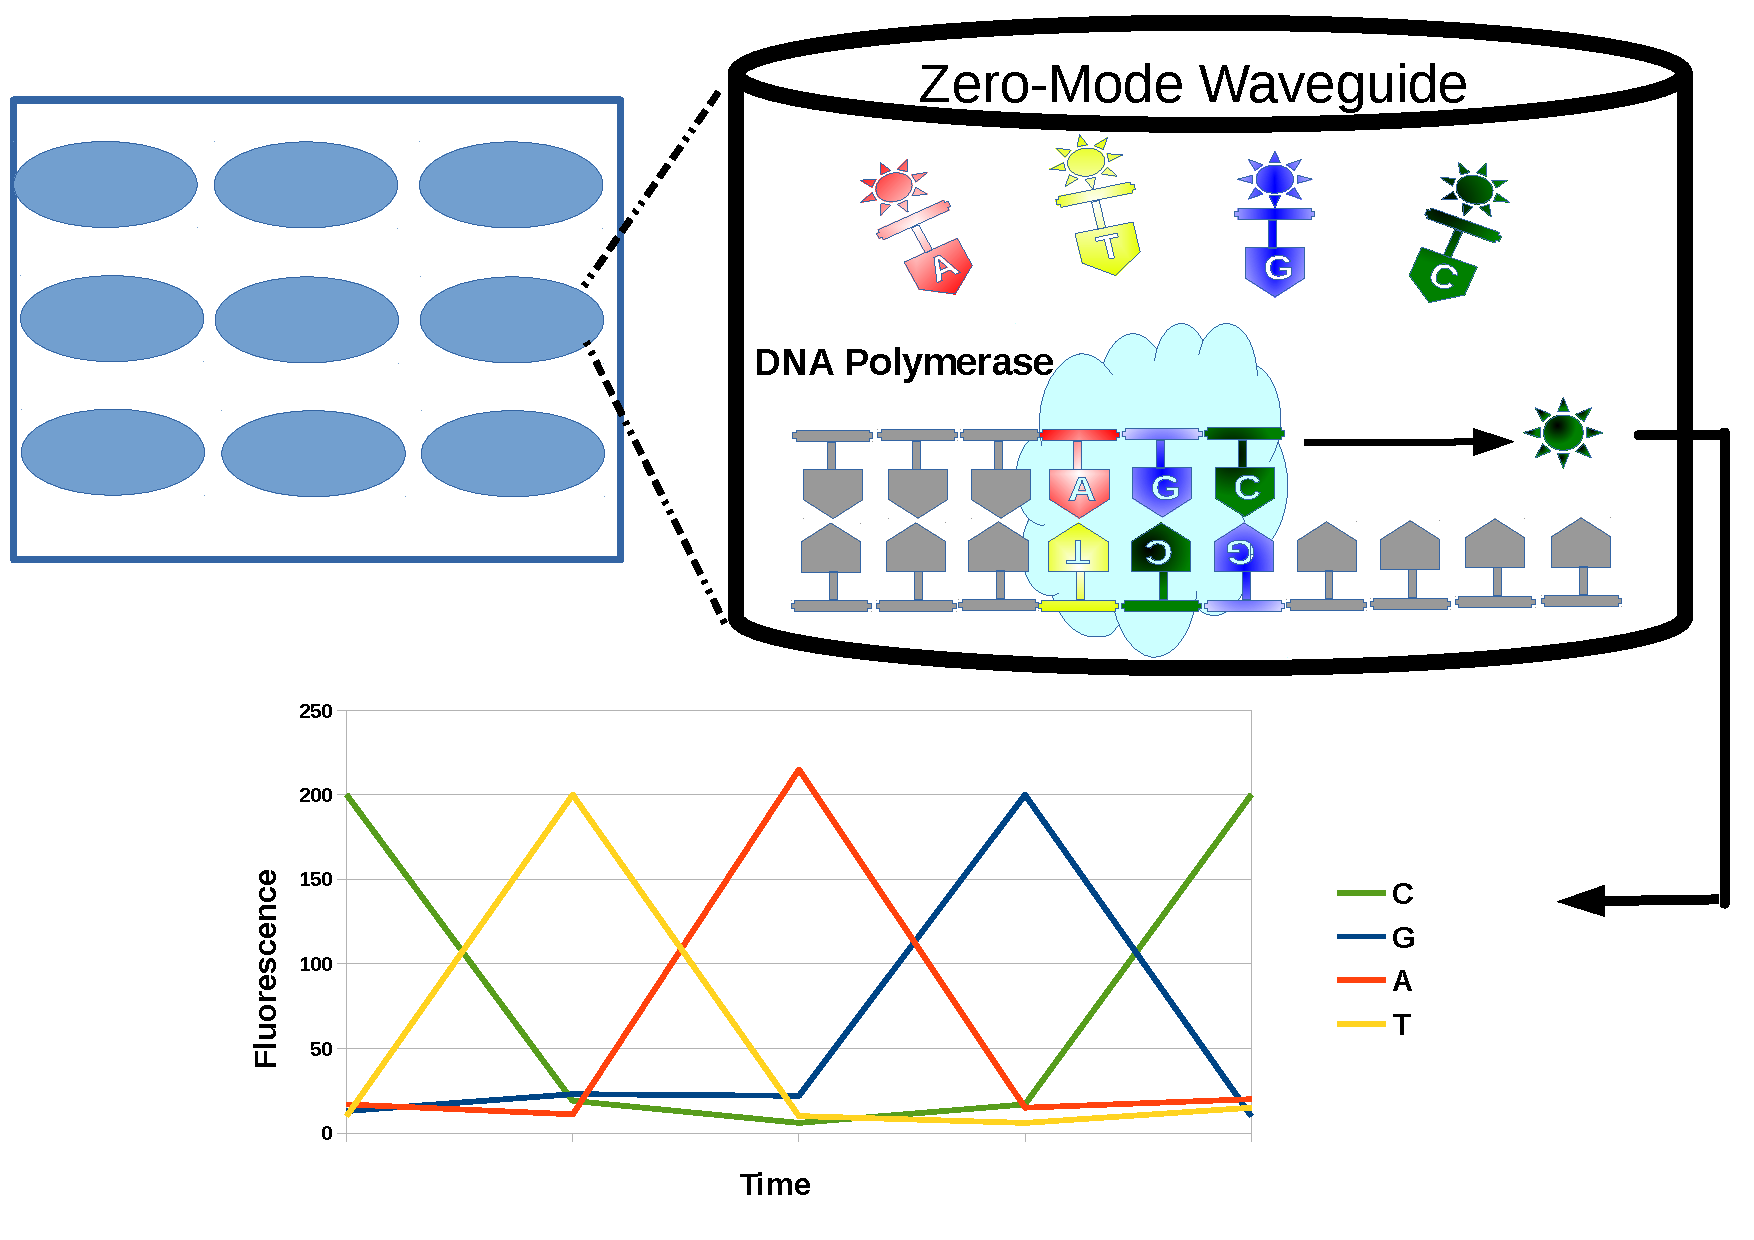
\includegraphics[width=.8\textwidth]{images/pacbio.pdf}
\caption{Mechanism of SMRT sequencing with Zero-Mode Waveguides.}
\label{F:pacbio}
\end{figure}

The SMRT technology takes advantage of \emph{zero-mode} waveguides (ZMW) to detect the activity of DNA polymerase incorporating a single nucleotide at a time \cite{Rhoads2015}. 
A ZMW structure consists of a circular hole in sub-wavelength scale ($20\times10^{-21}$ litre volume) in a metal film \cite{Korlach2008selective}. A complex of DNA polymerase and a single stranded template DNA molecule is immobilized at the bottom of the chamber surrounded by fluorescent dyed bases, as shown in Figure \ref{F:pacbio}. The DNA synthesis activity cleaves off the dyed tag of each incorporated base which can be detected optically in real-time within this smallest available microscopy structure \cite{Levene2003zero}. A SMRT cell can harbor thousands (RS platform) to hundred thousands (RS II) or even millions of ZMWs (Sequel, 8M chip) to facilitate parallelization and thus improve the throughput per cell. 

In fact, both the read length and accuracy of the instrument have been continuing to increase significantly. The average accuracy per read has increased from about 82\% in the first release to 87\% \cite{Eid2009,Koren2013} whilst the maximum read length has reached over $50$Kbp in recent runs \cite{Berlin2015}. 
As the consequence, PacBio DNA reads have gone from only being used in hybrid assembly which required high-fidelity complementary reads \cite{KorenSW2012, Ribeiro2012}, to now being able to generate finished \emph{de novo} bacterial genomes on its own \cite{Koren2013}.

\paragraph{Oxford Nanopore sequencing} 
In late 2013, ONT released the first nanopore sequencer, the \emph{MinION}, in the \emph{MinION Access Program} (MAP).
MAP was offering opportunity to researchers worldwide to have access on the third-generation reads. 
Of the particular advantages using this device is its greater portability and flexibility.

\begin{figure}[h]
\centering
\subfloat[Sequencing with MinION\label{fig:minion}]{
	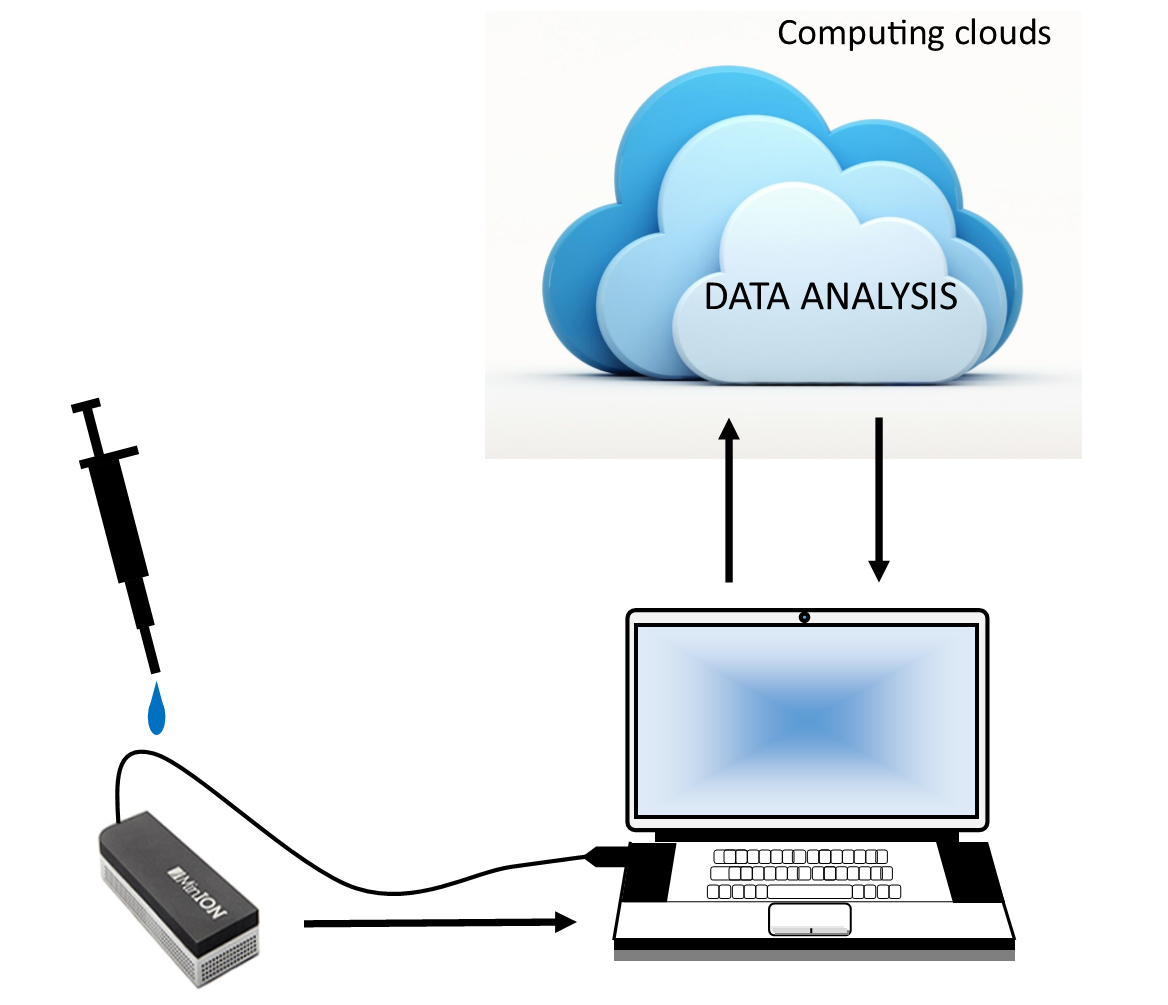
\includegraphics[width=.55\textwidth]{images/mnanopore.png}
}
\hfill
\subfloat[Inside the pore\label{fig:pore}]{
	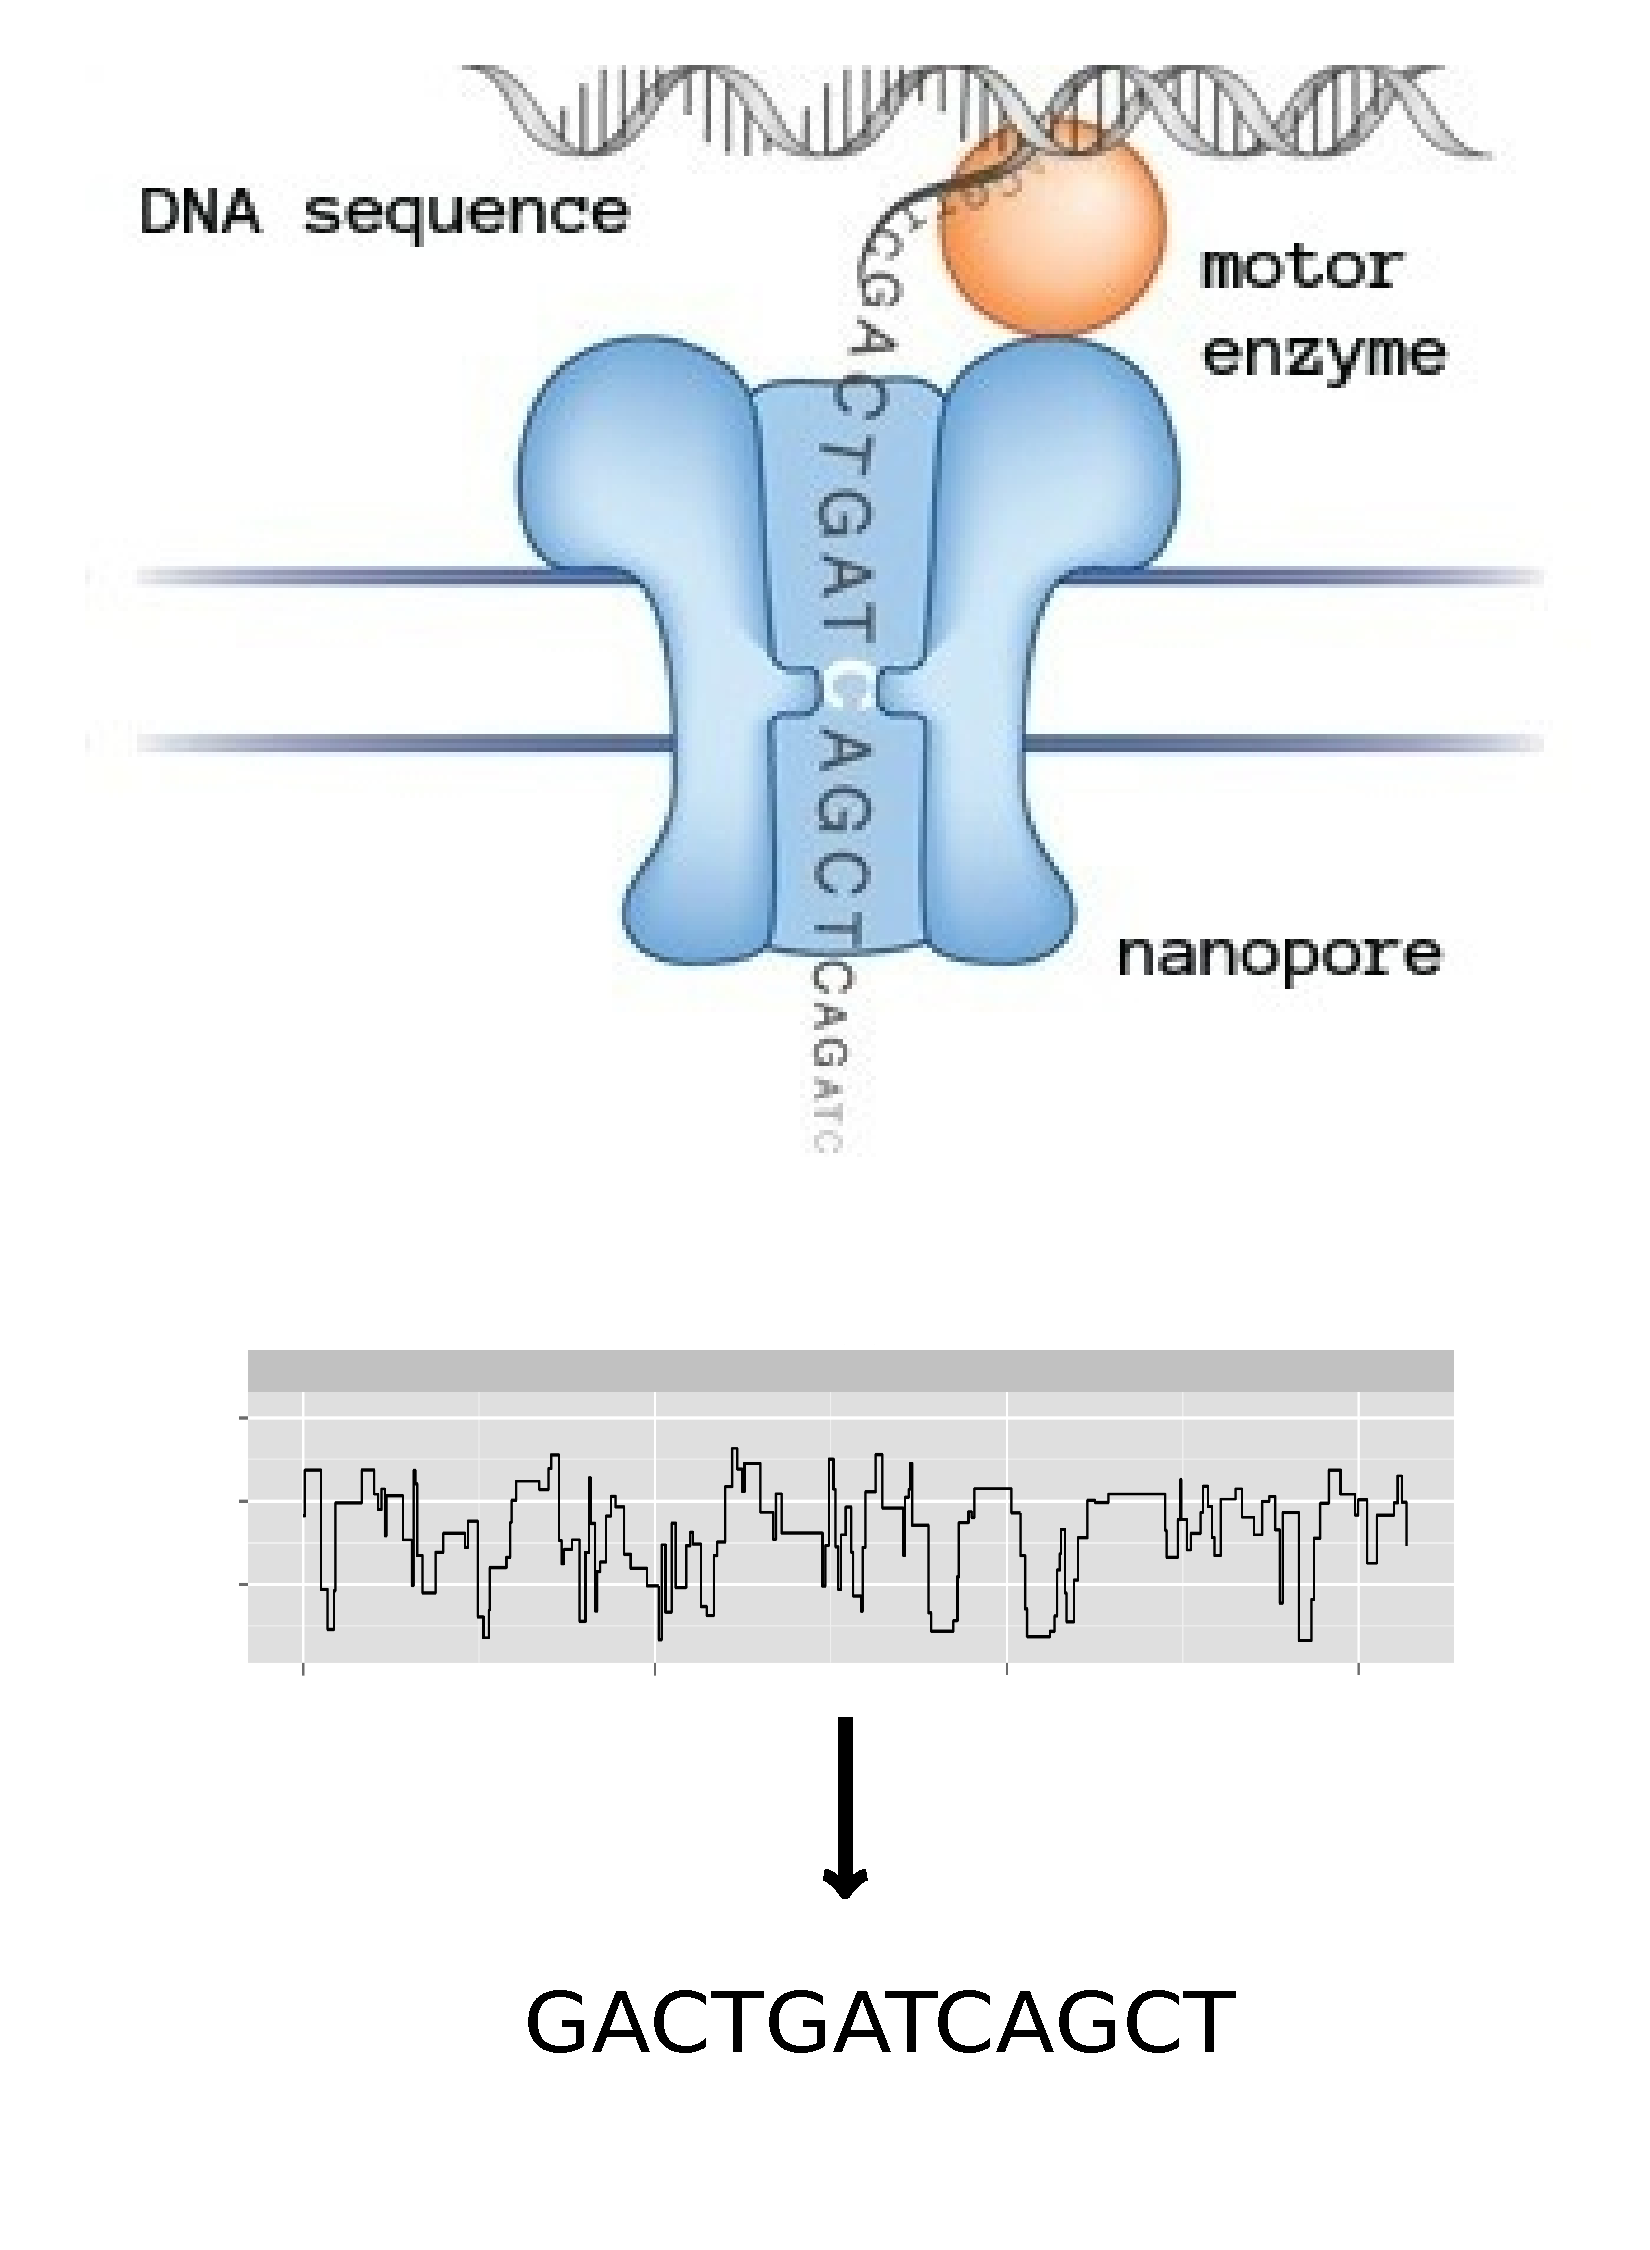
\includegraphics[width=.35\textwidth]{images/pore.pdf}
}
\caption[Illustration of nanopore sequencing with MinION]{Illustration of nanopore sequencing with MinION. (a) General setup for MinION sequencing. (b) Nanopore sequencing mechanism at molecular level.}
\label{F:nnp_run}
\end{figure}

Figure \ref{fig:minion} presents a general work flow of a sequencing run using MinION.
After DNA extraction, the very first step -- sample and library preparation, is straightforward but can also be varied for different experimental aims, such as maximizing yield, accuracy or read-length; as well as different experimental conditions, such as amount and quality of starting DNA.  
The purpose of library preparation is to bring necessary adapters and/or chemistry to the input mixture prior to the sequencing. 
ONT provides a variety of sequencing kits for different purposes.  For example, using the Rapid Sequencing Kit is simple and quick (10 minutes in theory) that would fit experiments with critical time and resource condition \EG{} remote locations. On the other hand, the Ligation Sequencing Kit family is more time-consuming  (about an hour) but gives better control over read length.
Other than these, ONT offers expansion packs for diverse project scenarios such as Barcoding kits for multiplexed sequencing or Low input kits for sequencing as little as $10$ng of DNA molecules.
In addition, if better quality is desired, users could, in the early stages, consider using a 2D kit (which would sequence both DNA strands in a single read), which has been replaced with an updated 1D$^2$ protocol (which with high probability sequences the second strand in the same pore immediately after sequencing the first strand, but as a separate read). 
After loading the prepared mixture to the device, the sequencing and base-calling phases could be employed automatically and \emph{in situ} thanks to the built-in services. In combination with a MinION, it is only required to have an internet-connected laptop with proper software installed to run the experiment, making it possible to establish sequencing-on-the-field where access to lab equipment is limited.

Figure \ref{fig:pore} illustrates the sequencing mechanism in more details.
In fact, the general mechanism of an artificial nanopore has been proposed \cite{Kasianowicz1996,Church1998} long before being applied as a real DNA sequencing technique by Hagan Banley and ONT \cite{Clarke2009}. 
In which, the unwound molecules are threaded through a nano-scaled pore on an electrically charged membrane protein known as \emph{the nanopore}. 
In the whole process, the velocity of the molecule translocating through the pore is controlled by a motor enzyme.
The rationale of this technology is that the shift of nucleotide sequence inside of a pore leads to the variation in its electrical resistance, resulting in a change in the current signal which is recorded as squiggles by time. These squiggle signals are feasibly translated back to the format of strings of nucleotide identities.
Indeed, a Hidden Markov Model (HMM) \cite{Baum1966,Baum1970} in the older version of Albacore, or Recurrent Neural Network (RNN) deep learning algorithm in later versions of Albacore, Chiron~\cite{teng2018chiron}, Guppy are used to study the transition and predict the sequence of DNA that most likely would generate these signals. 
Due to the  unavoidable noises of the measures in such tiny scale, a certain innate level of error may be expected from the base callers, although ONT has proposed using a variety of different types of pores simultaneously in order to generate independent error profiles. 

The nanopores are packed into a \emph{flow cell}, which is the consumable of this technology. Start-up cost of operating MinION is virtually zero, as users only have to pay for running costs, making it suitable for any project scale.  
The chemistry and computational features are likewise updated continuously to help reduce the noises from output. Recently, R10 flow cell is made available for higher signal accuracy, together with the newest base-calling algorithm from Guppy flip-flop pipeline that supports GPU for heavy computational deep-learning tasks, it has shown positive progress of this sequencing technology to tackle errors. When the demand of resources optimization is concerned, \emph{flongle} (single-use flow cell) can be used for small genomes. On the other hand, washing kits can be applied to reactivate pores from an interrupted flow cell, making it ready for another run.  

Furthermore, GridION and ProthmethION -- the scaled-up version of MinION, are made to public by the company through its access program and has already been deployed for several experiments involving bigger and more complicated genomes. This included human genome~\cite{De2019structural} and metagenomics mock community~\cite{Nicholls2019zymo} where data is available at \url{https://github.com/LomanLab/mockcommunity}.

In summary, ONT provides promising and fast-growing sequencing technology that could facilitate substantial applications in real-life.
The first description of the data generated by this sequencing method at early stage will be presented in the following section.
%%%%%%%%%%%%%%%%%%%%%%%%%%%%%%%%%%%%%%%%%%%%%%%%%%%%%%%%%%%%%%%%%%%%%%%%%%%%%%%%%%%
%%%%%%%%%%%%%%%%%%%%%%%%%%%%%%%%%%%%%%%%%%%%%%%%%%%%%%%%%%%%%%%%%%%%%%%%%%%%%%%%%%%
%%%%%%%%%%%%%%%%%%%%%%%%%%%%%%%%%%%%%%%%%%%%%%%%%%%%%%%%%%%%%%%%%%%%%%%%%%%%%%%%%%%
\section{Nanopore long-read data at first glance}

Together with PacBio RS series, the ONT MinION sequencing device, through its early access programme (MAP), has become a prominent long-read data generator for researchers worldwide. 
An initial interrogation on the Nanopore data generated by MinION over time here would provide first impression on its performance as well as the innovating progress that had been made to improve the output. 

\subsection{Data description}

\begin{figure}[ht!]
\centering
\subfloat[R6 (2014/06/16)\label{fig:r6}]{
  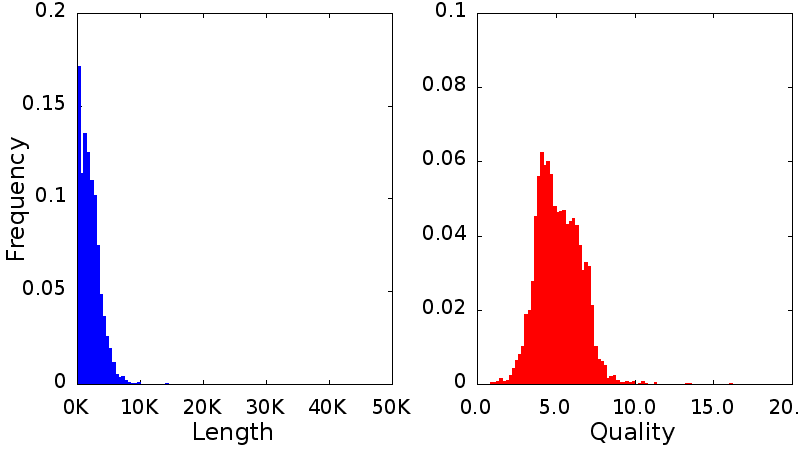
\includegraphics[width=.5\textwidth]{images/lambda_R6.png}
}
\subfloat[R7 (2014/09/16)\label{fig:r7}]{
  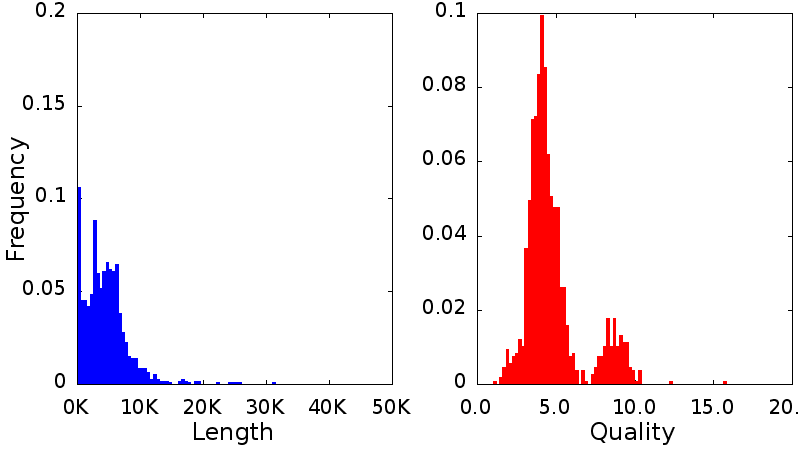
\includegraphics[width=.5\textwidth]{images/lambda_R7.png}
}

\subfloat[R9.4 (2017/01/18)\label{fig:r9.4}]{
  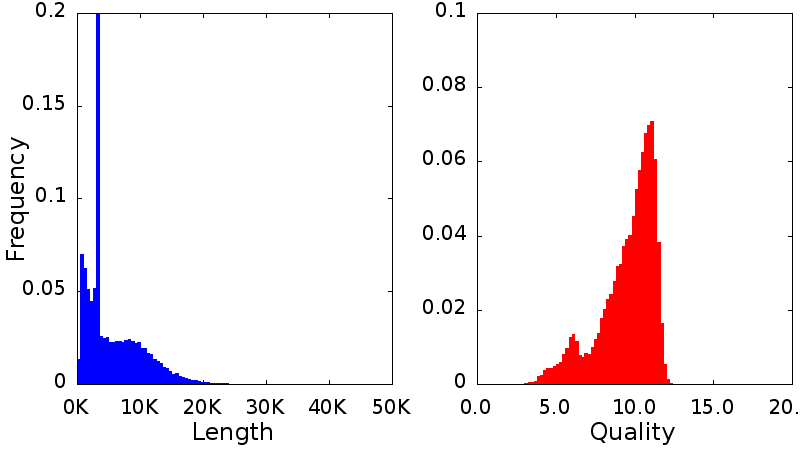
\includegraphics[width=.5\textwidth]{images/lambda_R9_4.png}
}
\subfloat[R9.5 (2018/09/12)\label{fig:r9.5}]{
  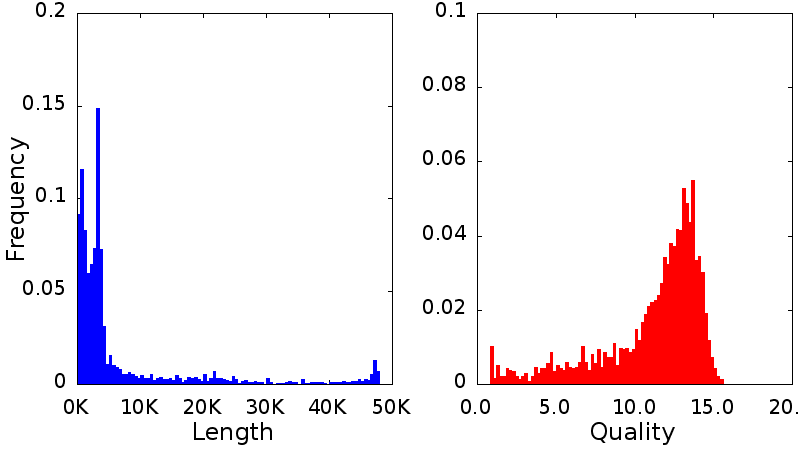
\includegraphics[width=.5\textwidth]{images/lambda_R9_5.png}
}

\caption[Statistics of nanopore burn-in experiments using different flow cell versions]{Statistics of nanopore reads using different flow cell versions (with the running date) on the lambda phage sample, shown in the order in which they were released. For each flow cell, the blue normalized histogram is for read length and red one is for quality (Phred score).}
\label{F:nnp_stats}
\end{figure}

\subsubsection{Lambda burn-in experiments} 
Figure \ref{F:nnp_stats} shows statistics of our lambda experiments acquired by using progressively more update version of MinION flow cells. This type of practice is a standard control `burn-in' experiment recommended by ONT to help users familiarize themselves with the protocol, the equipment and the result long-read data. The sample is a virus named lambda phage with small genome size of $50$Kbp. All the test experiments were run for 6 hours, except R9.5 with a 1-hour run so the sequencing yields are not included in the comparison and the histogram frequencies are normalized by the number of reads for each attempt. Even though the `burn-in' experiment is not designed to exhaustively study the potential length of nanopore reads due to the limit genome size of the sample, it is easily to see from the figure a clear improvement of read length distribution by applying newer version of flow cells. The early-staged (2014-released) flow cells and chemistry in the kit produced fewer reads longer than $10$Kbp, as could be observed from Figure \ref{fig:r6} and \ref{fig:r7}. 
This remarked value has become the mean length of reads generated by R9.4 flow cell which can even possibly reach $20$Kbp in extreme cases. 
Using the newest available flow cell R9.5 - even for just a 1-hour run - produced many more longer reads, including the maximum possible $50$Kbp reads that cover the whole genome.  
Similarly, the fidelity of the long reads has improved with the 2016-released R9 flow cells. The average quality scores (in Phred scale) of the base-called sequences have advanced from $5.0$ ($P_{error} \approx 0.3$) in R6 and R7 to $10.0$ ($P_{error} \approx 0.1$) in R9.4 and $13.0$ ($P_{error} \approx 0.05$) in R9.5. 
To further enhance the quality, reads from two complementary strands can be sequenced and computationally merged to produce a single double-checked 2D or 1D$^2$ read.
% Accordingly, the latest R9.5 pores and new base-calling algorithm can help improving the quality of long reads to around 95\% accuracy for single-stranded (1D) and are even aiming at 99\% for 1D$^2$ reads.  %%LC comment - not sure relevant what there aim is, better to stick to what has been achieved
Even so, noises will inevitably remain in nanopore reads as the result of measurement noise at nano-scale, as compared to high-precision data generated by SGS when the average Phred score is usually 30 or more ($P_{error} \leq 0.001$).

\subsubsection{The first runs with bacteria data} 

\begin{table}[ht!]
\centering
\small
\caption[Sequence two \emph{K. pneumoniae} strains with the MinION]{Sequence two \emph{K. pneumoniae} strains with the MinION. Figures generated by \npreader{} GUI \cite{CaoGC2016}.} 
\label{tab:first}
 \begin{tabular}{lccl}
 \hline
 \toprule
 \textbf{Strain} & \textbf{Phred Quality Scores} &\textbf{ Read Length Distribution} & \textbf{Emp. errors} \\
 \hline
   BAA-2146 & & & Del: 9.5\% \\ 
   (NDM-1 strain)& \multirow{4}{*}{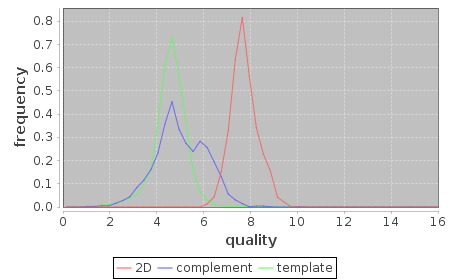
\includegraphics[width=0.33\textwidth]{images/qualR7.png}}    & \multirow{4}{*}{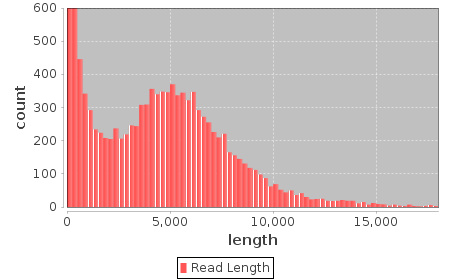
\includegraphics[width=0.33\textwidth]{images/lengthR7.png}} &  Ins: 6.3\% \\
    & & & Mis: 15.3\% \\    
   Chemistry R7& & &  Unaligned:  \\
   Sep 2014& & & \ \ \  13.3\% \\
   35-X Coverage& & & \\ \hline  
   
   13883 & & &  Del: 7.9\% \\   
   (type strain)& \multirow{4}{*}{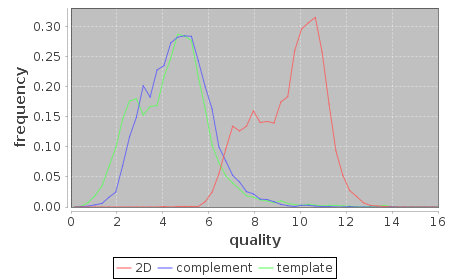
\includegraphics[width=0.33\textwidth]{images/qualR73.png}} & \multirow{4}{*}{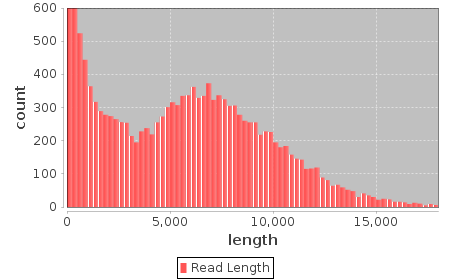
\includegraphics[width=0.33\textwidth]{images/lengthR73.png}} & Ins: 6.0\% \\
   & & & Mis: 12.9\% \\   
   Chemistry R7.3 & & & Unaligned:  \\   
   Dec 2014 & & & \ \ \ 11\%\\
   15-X coverage & & & \\ \hline
 \end{tabular} 
\end{table}

Amongst our first-hand experiments with real-life samples were the ones with \kp{} strains as shown in Table \ref{tab:first}. Flow cell version R7 and R7.3 with 2D sequencing protocol were used for the runs resulting in 35-fold coverage of long-read data for NDM-1 strain and 15-fold coverage for the type strain. From the quality histograms, the red lines represent 2D reads' scores which are clearly better than the ones in 1D reads (green and blue for template and complement sequences respectively). The length distribution shows that MinION sequencing returned significant reads with length around $5K$ for the first sample and $7K$ for the latter. The statistics on the far right of the table show error rate in term of indels, mismatches and hit rate from alignments with reference data. Overall, chemistry R7.3 is more up-to-date than R7 and as expected, gave slightly better results. 
As a next step, there came a mission to assembly those reads, together with available Illumina data of corresponding samples, in an attempt to have complete genome reconstructions for these two \kp{} strains. This task was important at the time as it would depict bigger picture about interactions between genetic elements in the whole genome and help to comprehend the biological pathways supporting this superbug's mechanisms.   

\subsection{Data analysis: challenges and solutions in working with nanopore data}
The introduction of long, error-prone nanopore reads has motivated novel developments in bioinformatics, as many existing approaches had been optimized for high-quality short read data.
A class of efforts was made to carry out an initial error-correction step before using the data set~\cite{GoodwinGE2015,MadouiEC2015}. 
This process usually require either another reference of high quality SGS reads or a large amount of long reads for self corrections.
The majority of algorithms following this approach uses alignment-based correction which is normally costly in term of computation.

Another attempt to reduce the error rate from base-called sequences is to utilize the signal-level information. Nanopolish is designed for such task. The underlying technique is to train a hidden Markov model that measures the probability of observing a certain chain of events given a particular DNA sequence. This method has been used for polishing a draft assembly using an abundance of long-read data~\cite{LomanQS2015} and has been extended to detect methylation~\cite{Simpson2017methylation}. Nevertheless, this approach is computational expensive and usually requires parallelization which is supported in its modules.

Pairwise sequence alignment is a critical operation for many genomics analyses in general and  comparative studies in particular. To adapt to the specific error characteristics of nanopore sequencing data, a number of approaches has been introduced on top of the legacy alignment methods used for short-read SGS data. 
The ubiquitous practice is still based on the previous seeds-and-extend dynamic programming technique with modifications in term of seed finding, gap extension and chaining algorithms. In addition, there would be justified settings to relax the matching criteria thus allowing more error tolerance and lengthen the alignments. As the results, early long-read alignment tools have been developed or calibrated for PacBio SMRT data, including but not limited to BLASR~\cite{ChaissonT2012}, LASTZ~\cite{Harris2007lastz}, LAST~\cite{KiełbasaWSH2011}, BWA-MEM~\cite{Li2013} and DAligner~\cite{Meyer2014daligner}.
Recently, several other tools has been designed specifically for comparing long-read data such as GraphMap~\cite{Sovic2016graphmap} and especially $\mathtt{minimap}$~\cite{Li2016} (now \minimap{}) which significantly reduce the running time while maintaining comparative accuracy at the same time.
These available solutions have been widely applied in a flexible ways for different analysis purposes when it comes to long reads with high error rate.

The problem of aligning raw long reads stems from the error profile per base in the targeting sequences, especially indels, that would introduce combinatorial explosion using traditional approaches. The common practice to tackle this problem is to apply \emph{hashing} techniques to reduce the dimensional of the data. A hash function maps a particular string to an index value so that it can be accessed directly without (or minimized) collision. By using these functions, a DNA sequences can be represented by a small set of fingerprints, known as sketch, that will be shared between similar but not necessary exact strings.
The prominent sketch types that has been used for nanopore data includes MinHash~\cite{Ondov2016mash,BerlinKC2015}, minimizer~\cite{Li2016}, HyperLogLog (\emph{Dashing: Fast and Accurate Genomic Distances with HyperLogLog} 
Daniel N Baker, Benjamin Langmead.
\textbf{bioRxiv} 501726; doi: \url{https://doi.org/10.1101/501726}
).

For the multiple sequence alignment (MSA) problem, the partial order alignment (POA) graph data structure has been proposed to cope with errors in long reads~\cite{Lee2002multiple,Lee2003generating,Grasso2004combining}. By applying this method, the authors proved the integrity of information compared to other MSA format and developed POA as an efficient tool for large alignment and consensus calling problem. The latter was then adopted in Racon~\cite{Vaser2017racon}, a commonly used consensus module for long uncorrected reads.

Genome assembly is another major challenge in bioinformatics when the traditional approaches for SGS data cannot be applied directly to TGS data.
To better understand the situations and come-up solutions, the general principle of genome assembly and methods for SGS data will be addressed in the next section.
Approaches to genome assembly which utilize nanopore reads will come later on top of this foundation knowledge. 

%%%%%%%%%%%%%%%%%%%%%%%%%%%%%%%%%%%%%%%%%%%%%%%%%%%%%%%%%%%%%%%%%%%%%%%%%%%%%%%%%%%
%%%%%%%%%%%%%%%%%%%%%%%%%%%%%%%%%%%%%%%%%%%%%%%%%%%%%%%%%%%%%%%%%%%%%%%%%%%%%%%%%%%%%
%%%%%%%%%%%%%%%%%%%%%%%%%%%%%%%%%%%%%%%%%%%%%%%%%%%%%%%%%%%%%%%%%%%%%%%%%%%%%%%%%%%%%
\section{Genome assembly}\label{sec:gass}
\subsection{Definition}
\begin{figure}[ht!]
\centering
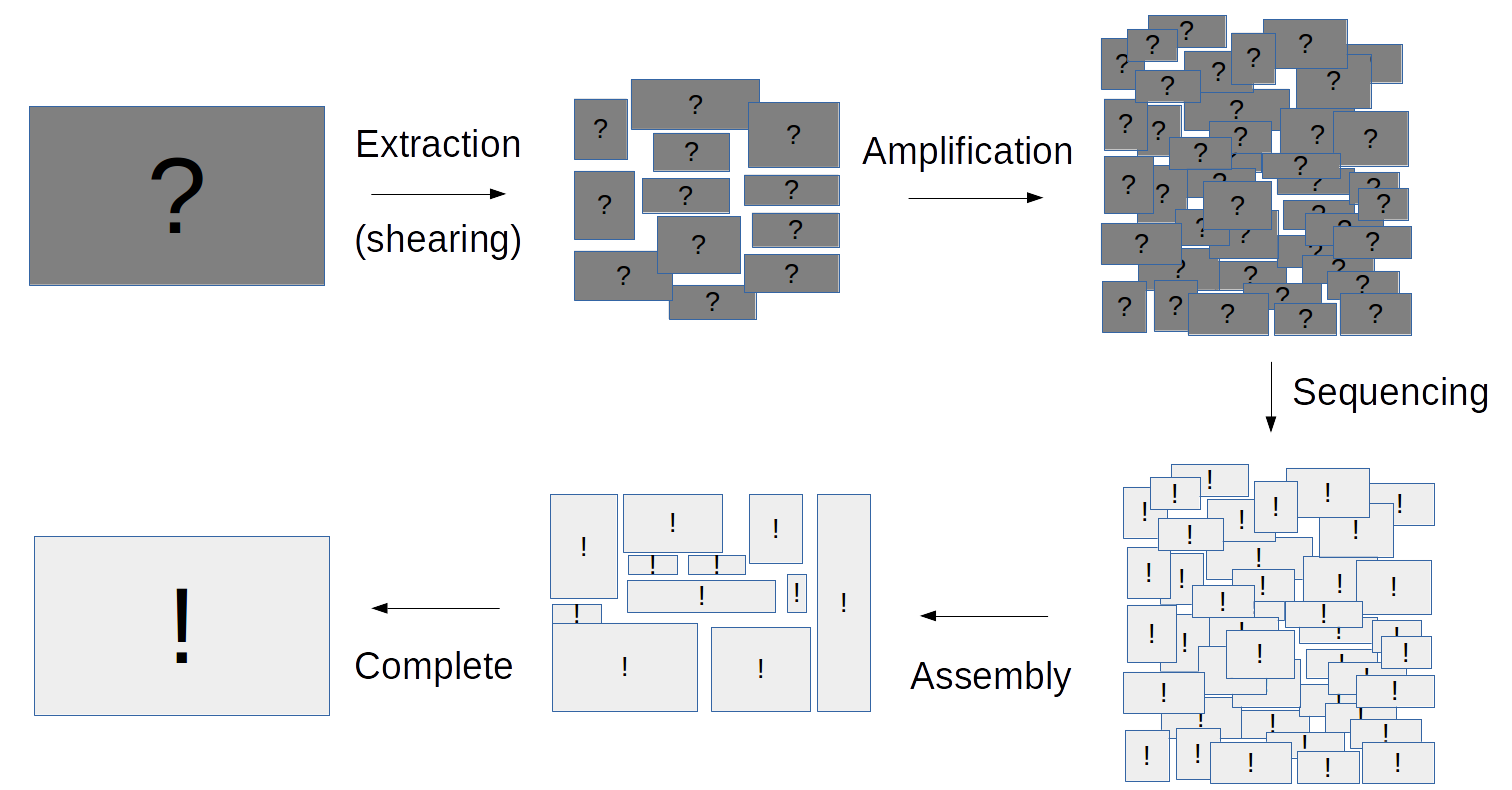
\includegraphics[width=.9\textwidth]{images/genome_decoding.png}
\caption{Basic framework for genome decoding process.} 
\label{Fig:decoding}
\end{figure}

Despite the huge improvements of sequencing technology, there still exist the common limitation that in most cases, it is impossible to sequence directly the whole length of a genome. As shown in Figure~\ref{Fig:decoding}, the actual practice is to break the whole genome into smaller pieces that could be efficiently read by an appropriate instrument. 
Before sequencing, the extracted DNA sample is normally sheared , \EG{} by restriction enzymes, into short fragments before being subjected to a cloning step, usually Polymerase Chain Reaction or PCR, that generates a large amount of copies for DNA molecules~\cite{Garibyan2013research}. The rationale is to have enough coverage to compensate the stochastic errors which are inevitable during library preparation and sequencing process. 
Those amplified pieces are then glued back together in a process called \emph{assembly} to have a draft genome prior to applications of additional post-processing steps for the final complete reconstruction.  
These include but not limit to scaffolding, gaps filling, genome polishing and circularizing if applicable.
The last two tasks are carried out with computational tools and in many cases, being referred together as in one whole common mission known as \emph{genome assembly}. 

Among all the steps involved in WGS, genome assembly undoubtedly plays a critical role in DNA sequencing since it determines how complete and accurate the picture of whole genome is. 



\subsection{General working principle for genome assembly}

\begin{figure}[ht!]
\centering
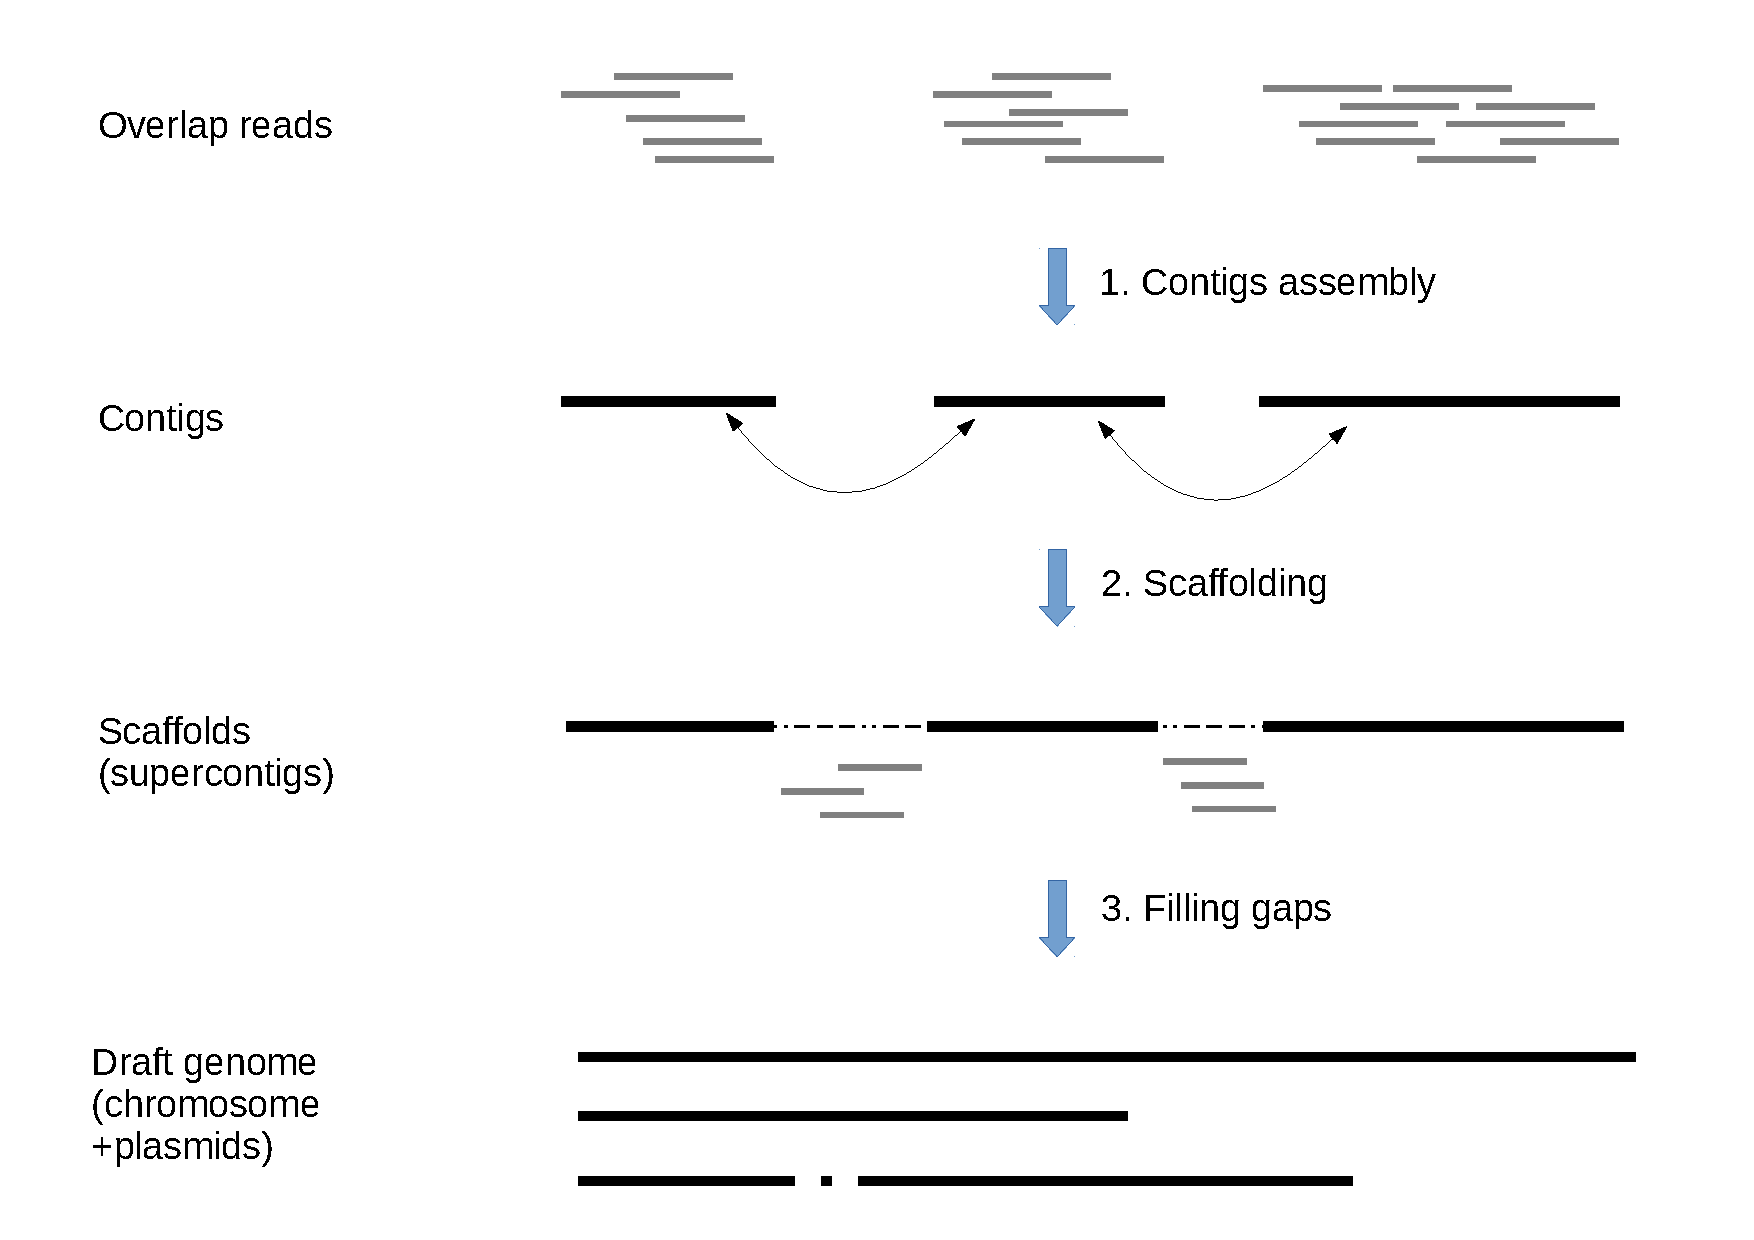
\includegraphics[width=.9\textwidth]{images/sassembly.pdf}
\caption{General assembly pipeline for short-read data.}
\label{Fig:assembly}
\end{figure}

A typical short-read assembly work flow would include three stages as shown in Figure \ref{Fig:assembly}. Firstly, the overlapping reads are merged together making up longer, un-gapped sequences named as contigs. Usually this is the most challenging and time-consuming part of the whole process, especially when the the number of reads is extremely large. The next step is to connect the fragmented contigs further by taking advantage of linking information from large insert reads \EG{} paired-end or mate pair data. The results are structures known as super-contigs or scaffolds that may contain estimated gaps. The final stage is to carefully fill those spaces by appropriate independent reads. The scaffolding and gap filling steps can be invoked repeatedly until no more improvement can be made \cite{Tsai2010improving,Boetzer2012toward,Paulino2015sealer}. The final result is a draft genome which consists of the longest possible stretch of sequences that can be induced from the data and algorithm. Unfortunately, it is common to not having the complete genome after this due to the repetitive nature of the DNA sequences. In fact, the fraction of fully completed genomes available in public databases such as GenBank (National Center for Biotechnology Information or NCBI) or European Bioinformatics Institute (EMBL-EBI), is comparatively small. Most of the assemblies are only near-completed, marked as contig- or scaffold-level, meaning that they are still fragmented and/or gap-bearing and require more work and data to become finished. 

\subsection{Overview of assembly algorithms for SGS data}
 
The demand for robust assemblers became overly compelling when high-throughput sequencing platforms were employed and started generating massive amount of data in the age of SGS.
The abundance of randomly distributed short reads from SGS platforms had motivated substantial research in bioinformatics toward solving the genome assembly problem in an efficient way\cite{Liu2012}. 
In general, approaches can be divided into two groups: greedy and graph-based approaches which are reviewed by \cite{MillerKS2010,LiZ2012}.
Greedy algorithms \cite{Sutton1995,Green1999,Huang1999} simply assemble all the reads by iteratively joining the two with largest overlap to form the shortest common string, or \emph{supersequence}.
It is noteworthy that greedy approaches implicitly use an overlapping graph as the data structure for this purpose. 
Clearly, the obtained result will be locally optimal and not necessarily the full solution to the problem. However, tools of this category usually produce a relatively good approximation \cite{Simpson2015}. 

The graph-based methods utilize data structure of vertices and edges to represent the whole set of reads and all of their potential linkage properties.
By traversing through the graph, one can define an assembly as an ordering reads and by searching for the best paths, find candidates for the optimal solution.
There are two types of graph in common use, namely Overlap--Layout--Consensus (OLC) \cite{Staden1979} and de Bruijin graph (DBG) \cite{Idury1995,PevznerTW2001}. 

\paragraph{Overlap--Layout--Consensus} The classical OLC algorithms follow the following three steps: overlap finding, layout forming and consensus calling. Throughout the process, an \emph{overlapping} graph is created which has vertices as reads and edges are represented by overlapped pairs of reads which have been detected based on alignments in the first step. A traversal algorithm is then applied to find the paths of ordered and oriented vertices, also known as the \emph{layout}. The consensus sequences are called and output based on the layout detected.
Among all the steps, finding overlap between all pairs of reads is the most computationally intensive. Although indexing techniques, such as FM index \cite{FerraginaM2005}, have been applied to reduce the time \cite{Ning2001}, the first step still remains the major bottleneck in the whole process, especially with the burst of short read data yield introduced by recent Illumina platforms.
In that circumstance, the DBG has come to be used as an efficient data structure to deal with this abundance of data. 

\paragraph{De Bruijin Graph} To construct the graph, reads are broken into consecutive \emph{k-mers} (words of length $k$) for the set of vertices, whilst edges show adjacencies between \emph{k-mers} with $k-1$ overlap. The data structure is actually storing fixed-length words and their linkages, making its memory requirement dependent only on the genome size but not data size. The graph is then targeted to errors removal based on \emph{k-mers} spectrum, as well as trimming and simplification in which non-branched paths are merged together.
At this point, the assembly problem can be reformulated as finding an Eulerian path which defined as a walk visiting each all edges on the simplified graph exactly once. 
The complexity of this algorithm is dependent on properties of the \emph{k-mers} rather than the number of reads. With a smaller $k$, the more details of overlaps emerge in the graph, but the trade-offs would be a bigger search space due to increasing number of nodes and edges. The reason for additional connections comes from the raise of repetitive elements not covered by the word length, resulting in more branches to traverse through the graph.  
Currently, there are several prominent DBG-based assemblers such as Velvet \cite{Zerbino2008}, SPAdes \cite{BankevichNA2012} and ABySS \cite{Simpson2009}. All of these work efficiently on Illumina HiSeq or MiSeq output with reasonable resources and running time requirements. In term of small genomes, such as bacterial genomes, which are the focus of this thesis, SPAdes is reported to be the most suitable tool amongst the three \cite{Magoc2013}.

\begin{figure}[ht!]
\centering
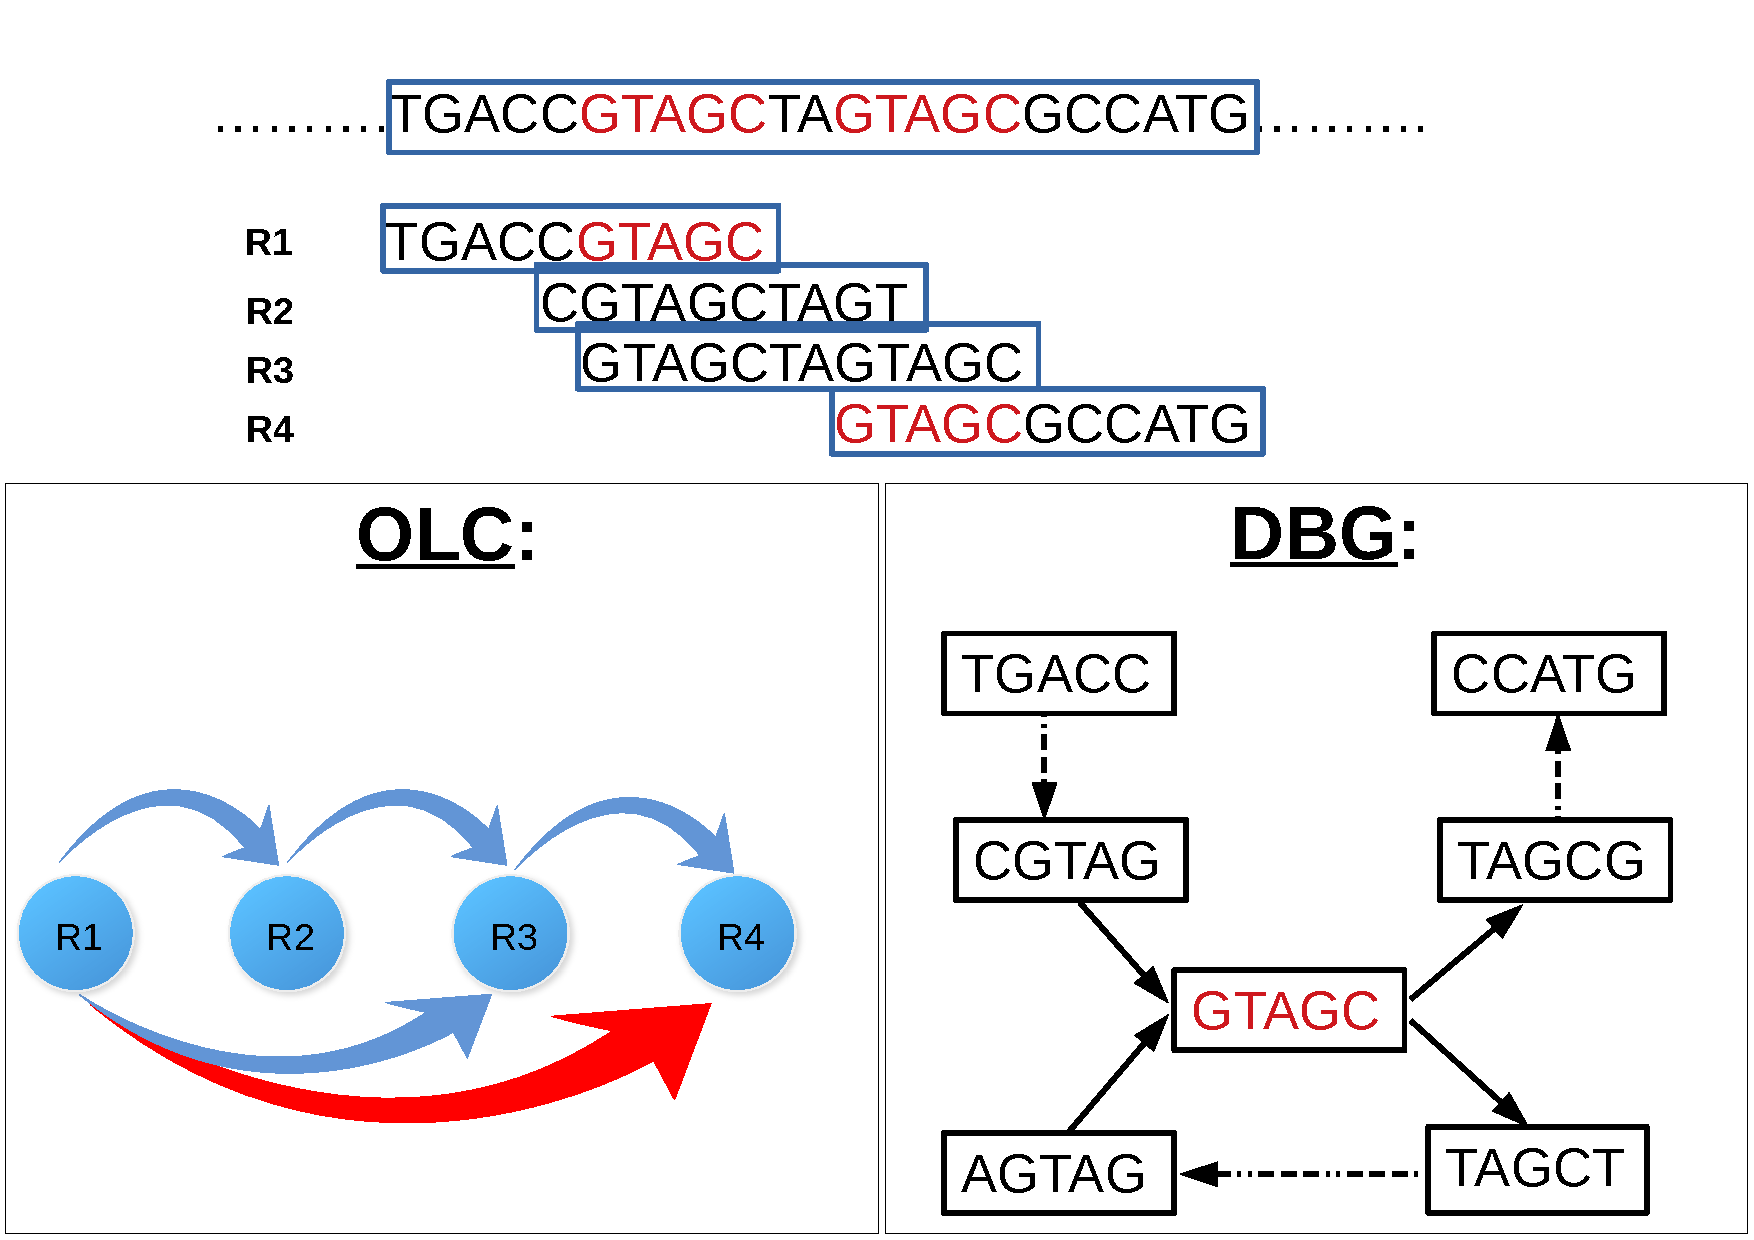
\includegraphics[width=.8\textwidth]{images/olcdbg.pdf}
\caption[Example about building OLC and DBG graph from a string]{A simple example about building OLC and DBG graph from a string with repeat (highlighted in red). The repeat introduces ambiguous alignment resulting in a redundant link (highlighted) in the overlap graph. It also de-linearizes the DBG graph by introducing a branched node corresponding to the repetitive \emph{k-mer}.}
\label{F:olcdbg}
\end{figure}

Figure \ref{F:olcdbg} gives an illustration of the graph construction by applying either the OLC or DBG approach.
A random string containing repetitive elements is given as the reference, from which reads are sampled as output from a short-read sequencer working on this imaginary genome. 
Using the OLC approach, a graph is built with reads as vertices and edges reflecting overlapping properties between pairs of them. Each time a new read is generated, there is one more vertex being added to the graph and by pairwise alignments to every other vertices, new edges can be added properly. To reduce size of the layout graph as the data set is growing, the algorithm usually tries to remove contained nodes and redundant edges, \EG{} $R2$ in the example since it is covered by $R1$ and $R3$ together. The repetitive elements cause additional faulty alignment, \EG{} the red link from $R1$ to $R4$, making it more complicated to traverse the graph in the correct sequence.

On the other hand, DBG approach first breaks reads into set of consecutive \emph{k-mer}s ($k=5$ in this case).
Unlike OLC, no pairwise alignments need to be explicitly carried out. 
As the consequence, the DBG graph is more efficient in term of construction, however, would be more challenging to solve compared to the reduced OLC graph. The reason stems from the fact that the integrity of reads are usually lost after being broken into smaller pieces as $k$ must be strictly less than the read length. 
At the same time, the repeat nature of original sequence would split the OLC nodes into extra branches compared to DBG counterparts, making it more fragmented and difficult to traverse.
It is worth to mention the importance of parameter $k$ for the DBG performance. 
As aforementioned, $k$ should be chosen as large as possible to restraint the loss of information and the complexity of the resulting graph. However the graph would suffer the risk of disjointed components, or dead-ends, if $k-mers$ becomes too long so that one word would less likely overlap with another by $k-1$.
From the example, we chose $k=5$ as the best option since the DBG with $k=6$ would fail to represent the overlap between R3 and R4.

As mentioned earlier, genome assembly from SGS data usually suffers from the presence of repeats, leading to generation of highly fragmented draft genomes (also known as pre-assemblies). This limits identification of structural variation, or identification of the configuration and location   of mobile genetic elements.
One theoretical solution is to have reads that exceed the `golden threshold' of $7000$ nucleotides to span over the majority of repeats in prokaryotes \cite{KorenP2015}, thus able to connect fragmented contigs and render continuous assemblies out of them.
In fact resolving repeats has remained a bottle-neck until the recent emergence of the so-called Third Generation Sequencing technologies with the introduction of two instruments PacBio RS and Oxford Nanopore MinION that were specially designed for long-read sequencing. Thanks to these sequencers, DNA molecules with continuous length of up to tens of kilo base-pairs or even more could be sequenced in full.
As a result, long-read data have been widely exploited to finish genomes \cite{BashirKR2013,KarlssonLS2015} or identify mobile genetic elements of interest \cite{HudsonBM2014,AshtonND2015}, despite having a higher base-calling error rate.
A class of assemblers using these new instrument's output has been developed, which I will describe in the following section.
%\vfill
%%%%%%%%%%%%%%%%%%%%%%%%%%%%%%%%%%%%%%%%%%%%%%%%%%%%%%%%%%%%%%%%%%%%%%%%%%%%%%%%%%%
%%%%%%%%%%%%%%%%%%%%%%%%%%%%%%%%%%%%%%%%%%%%%%%%%%%%%%%%%%%%%%%%%%%%%%%%%%%%%%%%%%%
\section{Genome assembly with long read data}
Nanopore data can be used on its own for \emph{de novo} genome assembly, or in conjunction with high quality SGS data in a process called hybrid assembly. 
Both approaches have their own pros and cons and should be considered in reference to available data set and the ultimate purposes of using the final assembly.
\subsection{Long-read only assemblers}
Non-hybrid assembly tools, as stated above, follow either OLC and/or an adjusted DBG approach, described below. Accordingly, most of current OLC algorithms rely on a hierarchical approach~\cite{Jayakumar2017compare}. From this perspective, seeds are first chosen top-down as a subset of longest reads that must have good base-called quality and not contain each others. The remaining reads of shorter length are then aligned to the seeds for error-correction before invoking assembly and post-processing as usual.

Hierarchical Genome Assembly Process (HGAP)~\cite{ChinAM2013} was one of the first hierarchical OLC tool available for PacBio data but a more well-known assembler in this category is \emph{Canu}, a renovated version of \emph{Celera Assembler}~\cite{MyersSD2000} that was designed to work in particular with noisy long sequences. Canu employs a typical OLC approach with an adaptive overlapping strategy and sparse assembly graph construction to be able to build a correct overlap graph out of error-prone data~\cite{Koren2017canu}. Canu is able to generate decent final assembly for large eukaryotic genomes but usually requires a lengthy running time.
FALCON~\cite{Chin2016facon} is another assembler applicable to big genomes, more than that, its string graph is designed to be diploid-aware.
Another efficient OLC implementation is to apply a fast overlap finding algorithm first for the assembly skeleton, then use another consensus calling or polishing tool on the draft assembly to improve the quality. This idea has been integrated in SMARTdenovo (\url{https://github.com/ruanjue/smartdenovo}) or in a pipeline that combines 2 separately developed modules: \emph{miniasm}~\cite{Li2016} as the rapid draft constructor and \emph{Racon}~\cite{Vaser2017racon} as the consensus caller. 
%%LC comment - is this a good time to discuss minhash and other hashing approaches, like hyperloglog


Regarding to other class, \emph{Flye}~\cite{Lin2016abruijin,Kolmogorov2019Flye}  and \emph{wtdbg} (\url{https://github.com/ruanjue/wtdbg2}) are two representatives of long-read assemblers that used adaptive versions of \emph{de Bruijin} graph.
The first method introduces the definition of ABruijin graphs that only take a subset of ``solid strings'' instead of all fixed length words decomposed from reads. The solid strings are chosen based on the \emph{k-mer} spectrum from which their fidelity are examined.
Unlike the traditional DBG methods, a fast dynamic programming algorithm is used to evaluate the overlaps of various lengths between read pairs based on their longest common subpaths. The draft assembly is constructed by adding vertices of those overlapped reads before undergoing a polishing step by aligning it to the original reads.
The tool wtdbg (now wtdbg2) on the other hand, builds a fuzzy de Bruijin graph for genome assembly. This graph is similar to the original DBG but allows mismatches and indels so that approximate \emph{k-mer}s can be collapsed into one node of the graph. Furthermore, the read paths are kept during decomposition and collapsing. After layout construction with the fuzzy DBG, a POA-like consensus step is invoked to generate the final assembly. 
The tool is reportedly able to quickly finish an assembly but consumes more memory than an original DBG approach due to the new graph structure. 

For exclusive long reads assembly, the quality of assembly is in general lesser than SGS counterparts, even after a polishing step. 
As the consequence, additional polishing steps with Illumina data is desired for higher accuracy in \EG{} for SNP callings projects.
Another approach is to utilize the erroneous long reads as the linker to connect the incomplete SGS assemblies~\cite{DeshpandeFP2013,BoetzerP2014}. Assemblers from this class usually require less long read coverage. Moreover, bridging operations are much less resource-consuming than aforementioned approaches.  I expand on these hybrid assemblers in the next section. 

\subsection{Hybrid assemblers}

Hybrid assembly using long reads is an economical and efficient approach to retrieve more complete genomes from the drafts since it requires less runs of the currently expensive third-generation sequencing. 
One of the first algorithms that takes advantage of long reads for hybrid assembly is Cerulean~\cite{DeshpandeFP2013}. By aligning the contig sequences from short read assembly to the long reads, it tries to build a \emph{skeleton graph} of long contigs connected together as the backbone and later accompany smaller contigs iteratively to the backbone to improve the assembly quality. This tool provides an efficient way of finishing the draft genomes in the sense of running time and memory usage.
Likewise, in term of assembling with long-read data, SSPACE-LongRead~\cite{BoetzerP2014} stands out as a widely-used software for this particular task. 
Briefly, the method relies on the BLASR~\cite{ChaissonT2012} alignments between long reads and the pre-assemblies which are normally contigs resulted from short-read assemblers.
Based on the linkages from the best alignments, a placement of these contigs into super-scaffolds is established. 
The scaffolds will undergone a post-processing step of final linearization and circularization before being used as the assembly output.
This approach provided a cost-effective reconstruction of bacterial genomes by using two libraries: one Illumina MiSeq or Roche-454 paired-end reads and one 50-folds long reads data from PacBio.
Although long reads from other sources, such as MinION, can also be used by these methods~\cite{Karlsson2015}, it usually requires extra works on parameter calibration.

In addition, another scaffolding algorithm, LINKS~\cite{WarrenYV2015}, uses a \emph{k-mer} approach to make use of long reads properties rather than an aligner to connect the draft genomes. This method  succeeded in improving the contiguity of ABySS genome
assemblies and could adapt to a certain scale of eukaryotic genome. However, the performance highly depends on the data quality so that for early-staged chemistry of Nanopore sequencing, only 2D reads screening and/or application of error-correction utilities are recommended beforehand.
In ligth of that, beside several dedicated genome scaffolding tools for MinION data as above, users can always utilize the traditional approach of using error-free short reads to correct the nanopore reads at base level. After that, the corrected long reads can be assembled by a conventional OLC algorithm in the next step. Nanocorr~\cite{GoodwinGE2015} and NaS~\cite{MadouiEC2015} are two representatives for this approach. Normally, these assemblers could provide assemblies of high quality per base but with much more expensive computations in exchange. 

Finally, another appropriate software for this purpose is Unicycler~\cite{Wick2017unicycler} which has been developed as the state-of-the-art. This application is in fact a set of tools including a combination of short-read assembly optimization, long-read only assembly, hybrid assembly, consensus calling and other post-processing steps for microbial genome assembly. It is designed to work with either short-read or long-read data but focuses on the hybrid algorithm that take advantage of both type of data sets. 
Its hybrid assembly module works in a likewise non-interactive (batch) mode on the whole bulk of input data, traverses the input assembly graph and returns a exhaustively polished assembly as the result. 
This method has been proved to generate high quality, very close-to-complete genome assemblies thanks to exhaustive computational steps but the running time, as a trade-off, is relatively long and is only efficient for microbial genomes. 
More details about this method will be provided later in Chapter~\ref{ch:npgraph} as a relevant content.
%%%%%%%%%%%%%%%%%%%%%%%%%%%%%%%%%%%%%%%%%%%%%%%%%%%%%%%%%%%%%%%%%%%%%%%%%%%%%%%%%%%
%%%%%%%%%%%%%%%%%%%%%%%%%%%%%%%%%%%%%%%%%%%%%%%%%%%%%%%%%%%%%%%%%%%%%%%%%%%%%%%%%%%
%%%%%%%%%%%%%%%%%%%%%%%%%%%%%%%%%%%%%%%%%%%%%%%%%%%%%%%%%%%%%%%%%%%%%%%%%%%%%%%%%%%
\section{Real-time analysis}
\subsection{Definition}
In circumstances of this thesis, the adjective ``real-time'' indicates  a high level of responsiveness of an analysis system in updating its environment status corresponding to inputs fed into the system~\cite{Phillips1966programming}.
The time gap from getting new input to the point of status being updated, or \emph{deadlines}~\cite{Ben2006principles}, is not necessary to be as close to zero as possible (immediate), but in reality a positive value limited by a reasonable upper-bound (nearly immediate).
The upper-bound is normally defined based on human temporal sensation \EG{} within minutes.

Briefly, real-time data analysis is the operation applied on the data in a prompt time interval to provide near-instantaneous output.
In contrast, a data processing system is known to work in ``batch mode'' if it collects all the input data before any any operation is applied. 
The result obtained from a batch analysis on the bulk of data is final and static, meaning it cannot be updated using another batch of data without rerunning the whole process.
Real-time applications usually involve a specific communications method namely \emph{data stream}. Streaming data is characterized by its continuously migration from a \emph{source} to a \emph{sink}, which are normally the consecutive modules in a real-time pipeline.
To implement instant response programs is a challenging task but in return, grants certain amount of advantages over traditional batch counterparts~\cite{Croushore2011frontiers}. 
This will be discussed later throughout the content of this thesis.
\subsection{Real-time analysis for nanopore sequencing}
One of the novel aspects of ONT's sequencing platforms is that the sequence data of each molecule is written to disk as soon as it is generated (with up to 2000 molecules being sequenced in parallel, each molecule progressing through the pore at $450$bp per second).    This is unlike SGS sequencing-by-synthesis platforms, which sequence billions of short reads in parallel, with each cycle (contributing an extra base) taking several minutes, with the data being provided in batch at the end of a run.

For this task, the raw data of a read must be retrieved and analysed while sequencing is still in progress. This offers the opportunity to obtain analysis results as soon as sufficient data are generated, upon which sequencing can be terminated or used for other experiments.
As the consequences, answers to the related genomics questions could be obtained \emph{in situ}, in an automated manner that saves considerable amount of time and resources compared to the conventional approaches.
Furthermore, streaming analysis can benefit from avoiding under- and over-sequencing which could result in either the generation of more sequence data than is required at greater cost, or a low quality assembly if insufficient data are generated. 

Several systems incorporating real-time feature of MinION data have been developed e.g. the cloud based platform Metrichor (Oxford Nanopore), work by Quick\etal{}~\cite{QuickAC2015} and MetaPORE~\cite{GreningerNF2015}, focusing on phylogenetic analysis of a sample. 
Importantly, it is worth noting the selective sequencing protocol, \IE{}``\emph{Read Until}'', which had been proposed and implemented~\cite{LooseMS2016} exclusively for nanopore sequencing, motivated by the idea that only DNA molecules of interest should be sequenced. In this proposal, the process could intervene the transition of DNA through the pore by reversing the pore bias to eject the one deemed as non-informative. To achieve this, an examination is carried out for each molecule by reading the real-time squiggle data from current changes caused by the transition and comparing this signal to a reference. This real-time feedback system would be important for target enrichment and background depletion sequencing \cite{Edwards2018real}. 

On the other hand, as a member one of the very first groups having access to MinION sequencing, I have been developing an in-house tool set to analyze the data for specific studies, focusing in streaming analysis on microbial genomics.  
The framework had been implemented with utilities ranging from initial analysis to handful of further identification processes such as species typing, strain typing and investigating antibiotic resistance profiles on microbes~\cite{CaoGE2016}. In such pipelines, \npreader{}~\cite{CaoGC2016} continuously scans the folder containing sequencing data in parallel with the MinION sequencing. It picks up base-called sequences as soon as they are generated, and a stream of reads is created to feed the  appropriate pipeline for further identification analyses. 
Different modules of a workflow can communicate to each other via the network sockets or inter-process redirection pipes provided by Unix-like operating systems.
In general, each module takes a stream of data of interest (\EG{} a read, an alignment) as input and carries out its task every time a given amount of data or waiting interval has passed. As a response, only relevant information is extracted to retain or forward to another module following the analysis. 
This data processing methodology can return results on-the-go and at the same time, only engages small memory footprint which is a clear benefit when working with large amounts of data, over long period of running experiment.  
Our tools are proved to be helpful in reducing the turn-around time for the clinical analysis and heading toward rapid diagnostic usage of MinION in real-life applications~\cite{Bialasiewicz2018rapid}.

However, there still exists a gap for a method that could scaffold and finish assemblies in a real-time fashion.  % as of MinION's output.
This has become the motivation for this thesis project which will focus on using nanopore data in the scaffolding and annotating feature of \npscarf{}, demultiplexing algorithm from \npbarcode{}, as well as assembly graph resolving in \npgraph{} - all working in real-time.

\section{Summary}
To sum up, for the time being, there are various DNA sequencing platforms available in the market, each of them embraces its own methodology and outputs different reads in term of length, accuracy, throughput and sequencing cost. Hence the choice for a sequencing method depends on the requirement from individual project and sometimes, users need to use several sequencers together on the same sample to obtain adequate data of interest. 
Amongst the sequencing options, ONT nanopore sequencing with MinION stands out as a remarkably portable and deployable long-read sequencer that offers real-time access to the sequencing output. The continuous upgrades of its flow cell and sequencing kits are indeed improving the quality and quantity of the long-read data, making this sequencing method a very welcomed additional player in the field.

MinION data has been shown to be a useful source of genomic data for various  studies thanks to its long-spanning and real-time accessible features. In the midst of those, genome assembly and strutural annotation are amongst the most common applications since this technology can bypass the fragmentations caused by repetitive elements that are difficult to resolve using the short-read seqeuncing. At the same time, the on-time accessibility of the data opens up the opportunity to establish  analyses in real-time, thus offering interactive management on resources during sequencing process.
\section{Thesis aims}
Inspired by the unique functionalities of nanopore sequencing technology, this thesis project aims to  develop real-time applications using MinION data, focusing on genome assembly pipelines for microbial isolates. The purpose is to have further complete assemblies, as much as possible, that would facilitate downstream annotations.

\paragraph{Goals setting} Initially, the project targets to implement a streaming pipeline to rapidly finish short-read assemblies using real-time MinION sequencing. 
It is aimed to join fragmented contigs with least input data as possible while at the same time, still able to producing high quality and complete sequences. 
The ability to run and to report completion status in real-time allows users to decide when to stop the sequencing prematurely thus open the possibility of saving time and cost for genome analyses.
In addition, hybrid assembly algorithm is expected to work on the assembly graph of the short-read assemblies to further improve the sensitivity and completeness of the final result. It would also provide users appropriate visualization for better interaction with the assembly pipeline in real-time.

On the other hand, it is desired to extend aforementioned pipeline for multiple samples at the same time, through a paralleling mechanism known as barcoded sequencing.
This technology is made available from ONT, via Barcoding kits, to allow pooling and sequencing of multiple libraries on the sample flow cell, which further enhances the versatility of the technology. The underlying mechanism is to ligate a unique oligonucleotide sequence, or \emph{barcode}, to the fragments of each DNA sample. Multiple samples can then be pooled together and sequenced in one flow cell. After that, the sequenced reads are demultiplexed into bins by examining the barcode portions on the reads. 
For this purpose, a streaming demultiplexer for barcode sequencing is developed.
The tool brings to MinION practitioners a flexible option to monitor a barcoded sequencing run as well as to integrate pooled sequencing into a streaming analysis pipeline.
Together with in-house software developments, their applications into real-life use cases are taken place. This would give better understanding about software performances as well as specifications on different data sets.

\paragraph{Contributions} 
This thesis resulted in several real-time processing modules that are able to assist genome assembly and annotation, including \npscarf{}~\cite{Cao2017scaffolding} \npbarcode{}\cite{Nguyen2017barcode} and \npgraph{}. 
All of these individual add-on modules were wrapped in a bigger framework that was specifically designed for nanopore data analysis, hosted in \url{https://github.com/mdcao/japsa}. 
The main contribution of this thesis regarding genome scaffolding and assembly can be found in a separate repository \url{https://github.com/hsnguyen/assembly} for the convenience of development and maintenance.

The source code of the whole project is made available and applied in numerous use cases internally as well as from community. Feedback from users and external data sources are treated with care to further improve the performance and functionality of the developing software. 

\paragraph{Restrictions}
The thesis mostly focuses on applications in microbial genomics as this is a clear use case for the applicability of real-time analysis particularly in diagnosis and identification of antibiotic resistance strains.  However, the methodologies developed in this thesis can be applied more broadly, and have been demonstrated on yeast genomes. Applications to metagenomics and eukaryotic genomes were attempted but not thoroughly studied thus not included in the scope of in this thesis.

Another limitation is that the developed assemblers are hybrid approaches, meaning an additional SGS run is required before using the tools. An exclusive long-read assembler is difficult to adapt to a real-time pipeline due to its intensive computation for the error-correction stage which usually requires bulk of data and heavy resources consumption.
\section{Thesis outline}
The main research chapters of this thesis are organized as follows.
\paragraph{Chapter 2}: 
This chapter presents the implementation of the very first pipeline for finishing genomes in real-time using MinION long reads and side applications through \npscarf{}.
\paragraph{Chapter 3}:
This chapter describes demultiplexing barcoded nanopore sequencing data with \npbarcode{} in real-time and its application. In addition, there is another use case of using different assembly strategies to finish four XDR \kp{} strains.
\paragraph{Chapter 4}: 
This chapter shows how to integrate assembly graph into the available pipeline from \npscarf{} to improve the assembly quality. This work results in \npgraph{} and relate applications.
\paragraph{Chapter 5}: 
This chapter introduces another computational analysis of MinION sequencing data for small circular genome assembly, such as for virus, bacterial plasmids. Data for two \emph{Caulimovirids} samples are shown to demonstrate the performance of proposed methods.

%%%%% First chapter for npScarf
\cleardoublepage
\chapter{Streaming assembly using Nanopore reads}\label{ch:npscarf}
\thispagestyle{empty}
\vspace*{\fill}
\epigraph{\emph{The speed of decision making is the essence of good governance.}}
{--Piyush Goyal}

\clearpage
%%%%%%%%%%%%%%%%%%%%%%%%%%%%%%%%%%%%%%%%%%%%%%%%
This chapter describes a unique streaming assembly strategy on MinION data that has been implemented in a tool named \npscarf{}. Its methodology allows completing the assembly in real-time together with the nanopore sequencing nature. Several experiments on different data sets are conducted for better illustrations of \npscarf{} performance and functionality. 
Comparisons with other methods indicate better quality from the results while at the same time, consume less resources and running time.

These research findings have been published in a journal manuscript under the digital object identifier (DOI):$\mathtt{10.1038/ncomms14515}$. The manuscript will be reproduced with minor changes and reformatting for the whole content of this chapter.
The Supplementary materials for this paper is shown in \App{app:npscarf}.

As the co-first author, I am a primary contributor to the project in term of conception and design, software development, data analysis as well as drafting the first version of the manuscript. 
Specifically, I have predominantly designed the streaming pipeline and implemented the algorithm as the main developer of \npscarf{}. 
I have also contributed significantly to the analysis and interpretation of the research data. 
Finally, I am the author of the first draft versions of the manuscript on which the publication is based.

\clearpage
%%%%%%%%%%%%%%%%%%%%%%%%%%%%%%%%%%%%%%%%%%%%%%%%
%%%%%%%%%%%%%%%%%%%% Paper %%%%%%%%%%%%%%%%%%%%%
%\pagebreak
\thispagestyle{empty}
\vskip36pt
{\raggedright\sffamily\bfseries\fontsize{20}{25}\selectfont {Scaffolding and completing genome assemblies in real-time with nanopore sequencing}\par}
\vskip20pt
{\raggedright\sffamily\fontsize{12}{12}\usefont{OT1}{phv}{m}{n} {
\textbf{Minh Duc Cao}\textsuperscript{1,$\ast$,+},
\textbf{Son Hoang Nguyen}\textsuperscript{1,+},
\textbf{Devika Ganesamoorthy}\textsuperscript{1},
\textbf{Alysha G. Elliott}\textsuperscript{1},
\textbf{Matthew A.  Cooper}\textsuperscript{1} and
\textbf{Lachlan J.M. Coin}\textsuperscript{1,$\ast$}
}\par}
\vskip10pt
{\raggedright\sffamily\fontsize{10}{12}\usefont{OT1}{phv}{m}{n} {
\textsuperscript{1}Institute for Molecular Bioscience, University of Queensland, 
St Lucia, Brisbane, QLD 4072 Australia \par
\textsuperscript{$\ast$}Correspondence: \href{m.cao1@uq.edu.au}{m.cao1@uq.edu.au} and \href{l.coin@imb.uq.edu.au}{l.coin@imb.uq.edu.au} \par 
\textsuperscript{+}These authors contributed equally to this work
}\par}
\vskip10pt
{\raggedright\sffamily\fontsize{12}{16}\selectfont  {Received 11 Jul 2016. Accepted 6 Jan 2017. Published 20 Feb 2017}\par}
\vskip10pt
{\raggedright\sffamily\fontsize{12}{16}\selectfont  
PMID: 28218240 \hskip15pt DOI:~\href{https://doi.org/10.1038/ncomms14515}{10.1038/ncomms14515}\par}
\vskip10pt
\paragraph{Abstract}\mbox{}\\
Third generation sequencing technologies provide the opportunity to improve
genome assemblies by generating long reads spanning most repeat sequences. 
However, current analysis methods require substantial amounts of sequence data and
computational resources to overcome the high error rates. Furthermore, they can
only perform analysis after sequencing has completed, resulting in
either over-sequencing, or in a low quality assembly due to under-sequencing. Here we
present \npscarf{}, which can scaffold and complete short read assemblies while the
long read sequencing run is in progress. It reports assembly metrics in real-time so
the sequencing run can be terminated once an assembly of sufficient quality is
obtained. In assembling four bacterial and one eukaryotic genomes, we show that
\npscarf{} can construct more complete and accurate assemblies while requiring less
sequencing data and computational resources than existing methods. Our approach
offers a time- and resource-effective strategy for completing short read
assemblies.
\clearpage
\pagebreak

\section{Introduction}

High-throughput sequencing technology has transformed genomics research over the
last decade with the ability to sequence the whole genome of virtually any
organism on the planet. Most sequencing projects to date employ short read
technology and hence cannot unambiguously resolve the repetitive sequences that
are present abundantly in most genomes. As a result, assemblies are fragmented
into large numbers of contigs and the positions of repeat sequences in the
genome cannot be determined. These repeat sequences often play important
biological roles; for example, they mediate the lateral transfer of genes
between bacterial species via pathogenicity islands and plasmids. Analysing
these regions is thus essential to determine key characteristics such as
antimicrobial resistance (AMR) or to identify highly pathogenic variants of many
bacterial species~\cite{AshtonND2015}.

Long read sequencing technologies, for example Pacific Biosciences' (PacBio) and
Oxford Nanopore MinION sequencing, allow users to generate reads spanning most
repetitive sequences, which can be used to close gaps in fragmented assemblies.
A key innovation of the MinION nanopore sequencing device is that it
measures the changes in electrical current as a single-stranded molecule of DNA
passes through the nanopore and uses the signal to determine the nucleotide
sequence of the DNA strand~\cite{KasianowiczBB1996, BrantonDM2008, StoddartHM2009}. 
As such, the raw data of a read can be retrieved and analysed
as soon as it is generated, while sequencing of other reads is
still in progress.
This offers the opportunity to obtain analysis results as
soon as sufficient data are generated, upon which sequencing can be terminated
or used for other experiments.

Several algorithms have been developed to utilise long reads for genome
assembly. \emph{de novo} assemblers such as the hierarchical genome assembly
process (HGAP)~\cite{ChinAM2013} and nanocorrect/nanopolish~\cite{LomanQS2015}
can assemble a complete bacterial genome using only long read sequencing data.
However, because of the high error rates in these sequencing technologies, this
\emph{de novo} approach requires substantial amounts of sequencing data and
extensive computational resources, mainly for polishing the genome assembly. 
Hybrid assemblers, which combine error-prone long reads with highly accurate
and cheaper short read sequence data, provide a more economical and efficient
alternative for building complete genomes. They can be classified into three
categories. \emph{de novo} methods such as Canu~\cite{BerlinKC2015} and
miniasm/racon pipeline~\cite{Vaser2017racon} employ fast approximate approaches to assemble a skeleton of the genome using long reads. The skeleton, often as erroneous as the raw reads, is then polished with high quality short reads. On the other hand, tools in the \emph{error-correction} category (\EG, PBcR~\cite{KorenSW2012}, Nanocorr~\cite{GoodwinGE2015} and NaS~\cite{MadouiEC2015}) correct long reads with high quality short reads before assembling the genome with the corrected long reads. Finally, the \emph{scaffolding} methods (SPAdes-hybrid~\cite{BankevichNA2012, AshtonND2015},
SSPACE-LongRead~\cite{BoetzerP2014, KarlssonLS2015} and LINKS~\cite{WarrenYV2015}) use long reads to scaffold and fill in gaps in the
assemblies from short read sequencing.

While these tools are reported to assemble high quality bacterial
genomes~\cite{Castro-WallaceCJ2016, IstaceFD2016}, they have not made use of
the real-time sequencing potential of the MinION; assembly of a genome can only
be performed after the sequencing is complete. This can lead to over-sequencing,
which incurs extra cost and time; or under-sequencing resulting in a low-quality
assembly. Here, we present \npscarf{}, the first hybrid assembler that can
scaffold and complete fragmented short read assemblies with sequence data
streaming from the MinION while sequencing is still in progress. 
In effect, \npscarf{} can fully utilise a sequence read within
minutes of it being generated. Furthermore, it continuously reports
assembly quality during the experiment so that users can terminate the sequencing 
when an assembly of sufficient quality and completeness is obtained.
We show that our method can generate more accurate and more
complete genomes than existing tools, while requiring less nanopore sequencing
data and computational resources. As such, \npscarf{} can be used to efficiently
control MinION sequencing in completing existing short read assemblies and in
hybrid assembly projects. More importantly, \npscarf{} can facilitate the
real-time analysis of positioning genomic sequences for time critical
applications such as in AMR investigation.
We show that the \npscarf{} can rapidly and accurately reconstruct genomic islands
carrying AMR genes that are fragmented in short read assemblies. It can also
identify AMR genes encoded in plasmids. These are among the main analyses to
understand the acquisition of AMR in pathogenic bacteria.


\section{Results}

\subsection{Algorithm overview}

\begin{figure}[ht]
\centering
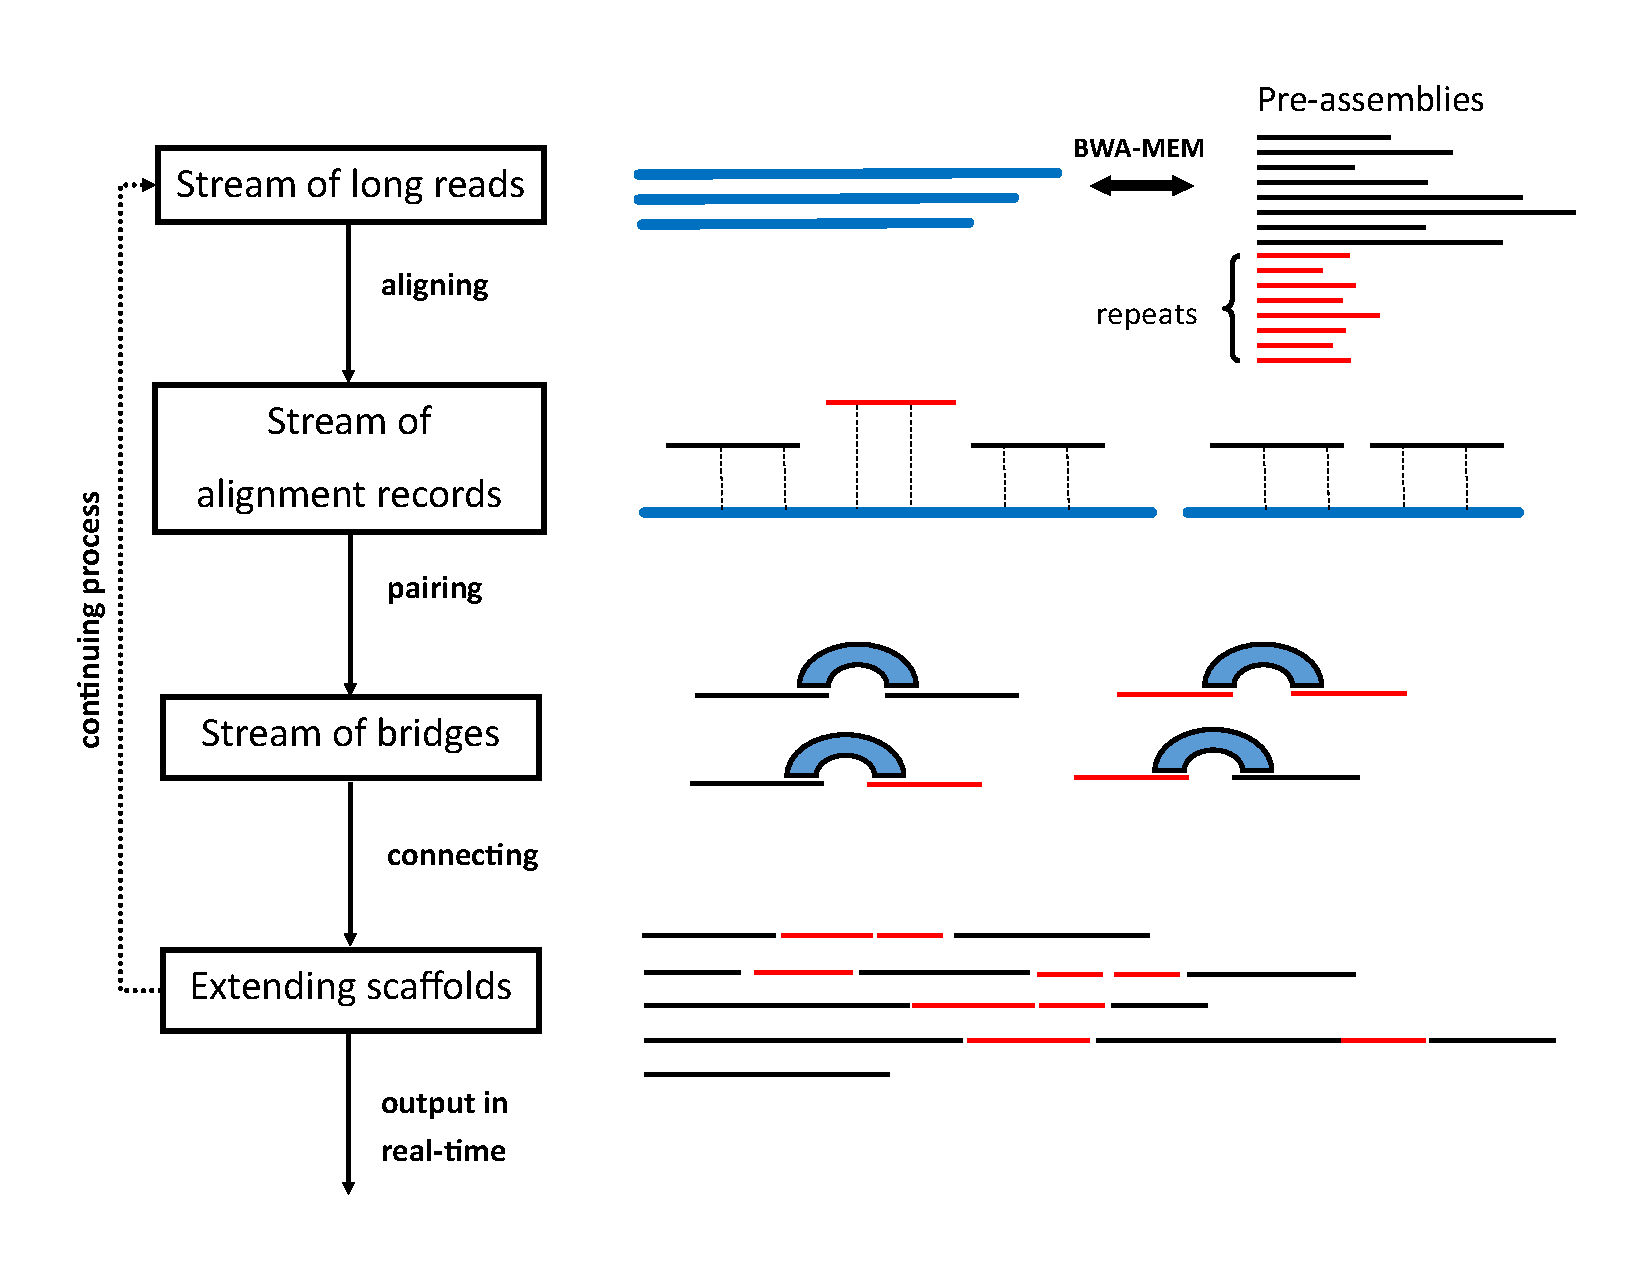
\includegraphics[width=\linewidth]{npscarf/figures/figure1.pdf}
\caption[Workflow of the real-time algorithm]{
Workflow of the real-time algorithm. Stream of long reads are aligned to the
existing contigs to create alignment records. Bridges connecting contigs are 
formed, and are used for extending scaffolds. These steps are performed in a
streaming fashion.}
\label{f:workflow}
\end{figure}

The genomes of most organisms contain an abundance of repeat sequences that are 
longer than the read length limit (300 bps) of Illumina sequencing 
platforms~\cite{TreangenS2012}. In assembling a genome using this technology, 
these repeat sequences cannot be distinguished and hence are often collapsed
into contigs, leaving gaps in the genome assembly. To complete the assembly, 
\npscarf{} first determines the multiplicity of each contig, thereby identifying
contigs representing non-repetitive sequences (called unique contigs).
It then scaffolds  and fills in gaps in the assembly in a streaming fashion
(Figure~\ref{f:workflow}). Upon receiving a long read from the MinION, \npscarf{}
immediately aligns it to the unique contigs. Reads aligned to two unique contigs
form a bridge connecting the two contigs. Gradually, the unique contigs are
joined to form the scaffold of the genome, while the repetitive contigs are
used to fill in the gaps in the scaffold. The details of the algorithms are
presented in Methods.

\subsection{Completing bacterial assemblies} 
\begin{figure*}[ht]
\centering
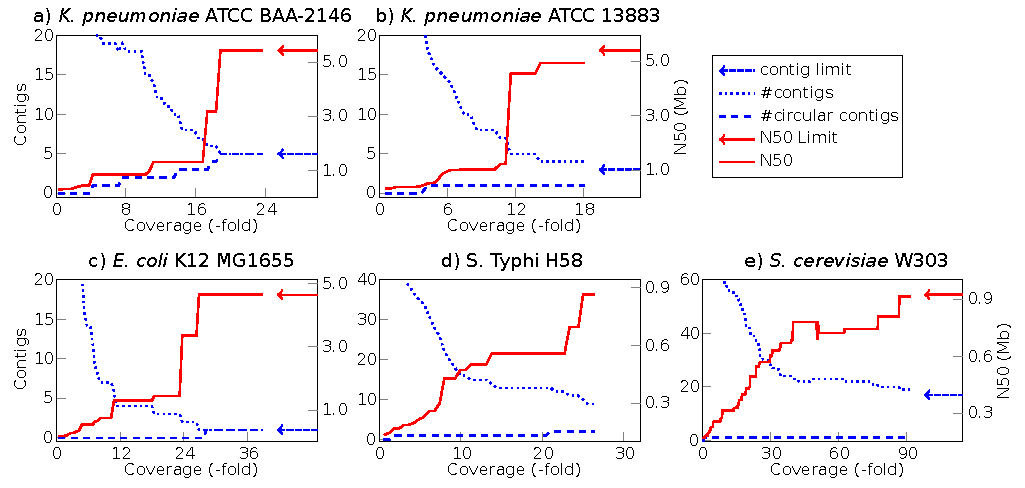
\includegraphics[width=\linewidth]{npscarf/figures/figure2.pdf}
\caption[Assembly statistics during real-time scaffolding]
{Assembly statistics during real-time scaffolding. 
The plots show N50 statistics, number of contigs, and number of
circular contigs against the amount of nanopore sequencing data.}
\label{f:scaffold}
\end{figure*}

\definecolor{Gray}{gray}{0.9}
\newcommand{\cir}{$^\ast$}
\newcommand{\bres}[1]{{\bf #1}}

\begin{table*}[ht]
\centering
\caption{Comparison between \npscarf's assemblies and the reference genomes of two \kp{} strains}
\label{T:alignment}
\vspace{5pt}
\resizebox{\textwidth}{!}{
  \begin{tabular}{llrlllrl}
  \hline
  \toprule 
  & \multicolumn{3}{c}{\textbf{\npscarf{} assemblies}} & &
  \multicolumn{3}{c}{\textbf{Reference sequences}}
  \\  
  \cline{2-4}
  \cline{6-8}
  & \textbf{Name}    & \textbf{Size (bp)} & \textbf{Plasmid \emph{ORI}}& &
  \textbf{Accession} & \textbf{Size (bp)} & \textbf{Plasmid \emph{ORI}}
  \\
  \hline
  \multicolumn{4}{l}{\kp{} ATCC BAA-2146} \\
  \rowcolor{Gray}
  \cellcolor{white} & 
  Contig 1\cir & 5,437,518 & - &  &  CP006659.1\cir & 5,435,369 & -   \\  
  \cellcolor{white} & 
  Contig 2\cir & 141,026 & IncA/C2 & & CP006661.1\cir& 140,825 & IncA/C2  \\  
 \rowcolor{Gray}
  \cellcolor{white} & 
  Contig 3\cir & 118,278 & IncFIB(K); IncFII(K) & & CP006663.1\cir& 117,755 &
  IncFIB(K); IncFII(K) \\
  \cellcolor{white} & 
  Contig 4\cir & 85,233 & IncR; IncFIA(HII) & & CP006662.1\cir& 85,164 & IncR;
  IncFIA(HII)  \\
  \rowcolor{Gray}
  \cellcolor{white} & 
  Contig 5\cir & 2,015 & ColRNAI & & CP006660.1\cir& 2,014 & ColRNAI  \\  
 \multicolumn{4}{l}{\kp{} ATCC 13883} \\
 \rowcolor{Gray}
  \cellcolor{white} & 
 Contig 1 & 4,923,970 & - & & KN046818.1& 5,284,261 & -   \\ 
 \rowcolor{Gray}
  \cellcolor{white} & 
 Contig 2 & 372,214 & - & & & & \\
   \cellcolor{white} & 
 Contig 3& 139,480 & IncFIA(HII); IncFIB(K) & & KN046820.1 & 95,930 &
 IncFIA(HII); IncFIB(K)  \\
   \cellcolor{white} & & & & & KN046821.1 & 42,420 & -   \\ 
  \rowcolor{Gray}
   \cellcolor{white} & 
Contig 4*& 119,388 & ColRNAI; IncFII(pCoo); pSM22 & & KN046819.1 & 106,842 &
IncFII(pCoo); pSM22  \\
 \rowcolor{Gray} 
  \cellcolor{white} & 
 & & & & KN046822.1 & 16,331 & -  \\
  \hline
\multicolumn{3}{l}{\cir Circular sequences.}
  \end{tabular}
 }
 
\end{table*}


We assessed the performance of our algorithm for its ability to scaffold and complete the
Illumina assemblies of two bacterial \emph{Klebsiella pneumoniae} strains, ATCC
BAA-2146 (New Delhi metallo-beta-lactamase (NDM-1) positive)
and ATCC 13883 (type strain).
We first sequenced the genomes of these strains with the Illumina MiSeq platform to 250-fold
coverage and assembled them with SPAdes~\cite{BankevichNA2012}
(See Methods). This resulted in assemblies of 90 and 69 contigs
that were 500bp or longer, respectively. The N50 statistics of the two
assemblies were $288$Kbp and $302$Kbp, respectively.
We then sequenced the two strains with Oxford Nanopore MinION using chemistry R7. 
For ATCC BAA-2146, we obtained $185$Mbp of sequencing data ($\sim$33-fold
coverage of the genome), of which $27$Mbp were two-directional (2D) reads. The run for strain ATCC
13883 yielded only $13.5$Mbp of sequencing data ($\sim$2.4-fold coverage). 
We re-sequenced this strain with the improved chemistry R7.3.
By combining sequencing data from both experiments for this strain, we obtained
a total of $100$Mbp ($\sim$18-fold coverage) data, including $22.5$Mbp of 2D reads.
The quality of the data, described in~\cite{CaoGE2016}, was broadly
similar to that reported by other MinION users~\cite{LomanQ2014, AshtonND2015,
JainFM2015}.

As the pipeline described here was developed after we performed the MinION
sequencing runs, we tested our streaming analysis by re-running the base-calling
using the Metrichor service. Sequence reads in fast5 format were written to disk,
and were instantaneously picked up and streamed to the pipeline by
npReader~\cite{CaoGC2016}. In essence, the scaffolding pipeline received
sequence data in fastq format in a streaming fashion as if a MinION run was
in progress. 
During analysis, the pipeline continuously reported the assemblies'
statistics (the numbers of contigs and the N50 statistic), allowing us to track
the completeness of the assembly, as well as the number of circular sequences in
the genome. This is especially important for the analysis of bacterial genomes
where chromosomes and plasmids are usually circular.
To validate the resulting assemblies, we compared them with the reference
genomes of these strains obtained from NCBI (GenBank Accessions GCA\_000364385.2
and GCA\_000742135.1). We also ascertained the predicted plasmids in these
assemblies by looking for the existence of plasmid origins of replication
sequences from the PlasmidFinder database~\cite{CarattoliZG2014}.


Figure~\ref{f:scaffold}a) and ~\ref{f:scaffold}b) present the progress of 
assembly completion against the coverage of MinION data during scaffolding.
As expected, N50 statistics increased and the number of contigs 
decreased with more MinION data. For \kp{} ATCC BAA-2146, we found that
our algorithm required only 20-fold coverage of sequence data ($<120$Mbp) to
complete the genome, reducing the assembly to the limit of five contigs (one
chromosome and four plasmids). Those five contigs were circularised, indicating
completeness. We found these five contigs to be in total agreement
with the complete genome assembly of the strain, previously sequenced with PacBio and
Illumina~\cite{HudsonBM2014} (See Table~\ref{T:alignment} and Supplementary
Fig. 1).


With 18-fold coverage of the MinION data for \kp{} ATCC 13883, the
assembly was improved to four contigs, in which one was reported to be circular
(Contig 4). These contigs were aligned to the reference genome for this strain, 
which contained 16 contigs in five scaffolds. We found Contig 1 and Contig 2
from the \npscarf{}'s assembly were aligned to the reference scaffold KN046818.1,
while Contig 3 and Contig 4 were aligned to two reference scaffolds (See
Table~\ref{T:alignment} and Supplementary Fig. 2). The
alignments contained forward and reverse matches. The breakpoints of
these matches corresponded to the contig joints in the reference scaffolds,
indicating the incorrect orientation of contigs in the reference scaffolds. 
The reference scaffold KN046818.1 was $5.2$Mbp in size, suggesting 
this scaffold was the
chromosome and was fragmented into two contigs in the \npscarf{}'s assembly. In
examining this chromosomal sequence, we found the two contigs to be separated by an 
rRNA operon of $7$Kbp in length. BLAST search revealed the structure of this operon
with rRNA 5S, 23S and 16S as the main components. This rRNA operon sequence was
also found to be present at five other loci in the genome, which were all
resolved. However, no long MinION read was found to align to this
particular position, possibly because of the low yield of this dataset, which
caused the chromosome sequence to be fragmented. 
We anticipate this could be resolved with more nanopore sequencing data.
Contig 3 ($139$Kbp) and Contig 4 ($119$Kbp) contained several
origin of replication sequences (See Table~\ref{T:alignment}), suggesting they 
were plasmid sequences; Contig 4 was also reported to be a circular sequence.
In Contig 4, we noticed an extra plasmid origin of replication sequence (ColRNAI) that
was not found in the reference genomes (see Table~\ref{T:alignment}).
In examining the position of ColRNAI, we found it was
in one of the gaps in the reference scaffold, hence not reported in the
reference assembly.

\subsection{Real-time analysis for positional information}

\begin{figure*}[ht]
\centering
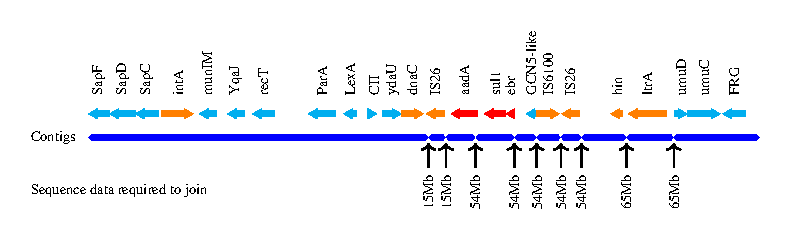
\includegraphics[width=\linewidth]{npscarf/figures/figure3.pdf}
\caption[Structure of a pathogenic island from \kp{}
ATCC BAA-2146]
{Structure of a pathogenic island from \kp{} ATCC BAA-2146. The island harbours three antibiotic resistance genes \emph{strep}, \emph{sul1} and \emph{ebr}, flanked by mobility genes integrase (\emph{int}), inverstase (\emph{hin}), DNA replication (\emph{dnaC}), and insertion sequences (IS26 and IS6100). The island was fragmented into 10 contigs in the Illumina assembly, and was completely resolved with $65$Mbp out of the total of $185$Mbp of nanopore sequence data.}
\label{F:gi}
\end{figure*}


\begin{table*}[!htb]
\centering
\caption{Timeline of determining plasmid-encoded antibiotic resistance genes}
\label{T:plasmidGenes}
\vspace{5pt}
\resizebox{\textwidth}{!}{
\begin{tabular}{cllll}
 \toprule
 Data \\
 required & Gene ID & NCBI ref & Antibiotic resistance & Plasmid evidence\\
\hline
$10$Mbp & blaTEM-1B & JF910132 & penicillins, some cephalosporins & IncR;IncFIA(HI1) \\
      & strB & M96392 & streptomycin & IncR;IncFIA(HI1) \\
      & strA & AF321551 & streptomycin & IncR;IncFIA(HI1) \\     
      & sul2 & GQ421466 & sulfonamides & IncR;IncFIA(HI1) \\
$14$Mbp & aac6Ib & M21682 & tobramycin, amikacin, netilmicin, sisomicin & IncR;IncFIA(HI1) \\
$21$Mbp & mphA & D16251 & erythromycin & IncFIB(K);IncFII(K) \\ 
      & tetA & AJ517790 & tetracyclines & IncFIB(K);IncFII(K) \\
      & QnrB7 & EU043311 & quinolones & IncR;IncFIA(HI1) \\
$29$Mbp & dfrA14 & DQ388123 & trimethoprim & IncR;IncFIA(HI1) \\ 
$46$Mbp &  blaNDM-1 & FN396876 & penicillins, cephalosporins, carbapenems & IncA/C2 \\
$51$Mbp & rmtC & AB194779 & aminoglycosides (include gentamicin, kanamycin) & IncA/C2 \\
$78$Mbp & sul1 & AY224185 & sulphonamide & IncA/C2 \\
      & aac6Ib\_1 & M21682 & tobramycin, amikacin, netilmicin, sisomicin &
      IncA/C2 \\
      & blaCMY-6 & AJ011293 & penicillins, some cephalosporins & IncA/C2\\
$83$Mbp & blaSHV-11 & GQ407109 & penicillins, some cephalosporins &  IncR;IncFIA(HI1) \\ 
      & aac6Ib & M21682 & tobramycin, amikacin, netilmicin, sisomicin &
 IncR;IncFIA(HI1) \\
      & blaOXA-1 & J02967 & penicillins & IncR;IncFIA(HI1) \\
      & aac3-IIa & X51534 & gentamicin, tobramycin, netilmicin, sisomicin &
 IncR;IncFIA(HI1) \\
     
\hline
\end{tabular}
}
\end{table*}

The ability to complete genome assemblies in streaming fashion also enables
real-time analyses that rely on positional information. Such analyses include
identifying genes encoded in bacterial genomic islands and plasmids. These
functional regions in the bacterial genomes can be horizontally transferred
between organisms, which is one of the main mechanisms for acquiring AMR in
pathogenic bacteria. Here we demonstrate these analyses on the multi-drug
resistant \kp{} ATCC BAA-2146 strain.

Prior to scaffolding the Illumina assembly of the sample, we annotated the
assembly using Prokka~\cite{Seemann2014} to identify the positions of genes and
insertion sequences in the assembly. Bacterial genomic islands are genomic
regions longer than $8$Kbp, containing certain classes of genes such as AMR genes.
In addition, they often carry mobility genes such as transposase, integrase and
insertion sequences (IS)~\cite{LangilleHB2010}. These sequences generally
appear multiple times in the genomes (repetitive sequences), causing genomic
islands fragmented in the short read assembly. We ran Islander~\cite{MantriW2004}
and PHAST~\cite{ZhouLL2011} on the Illumina assembly, which together detected
six genomic islands. In the annotation, we also found 28 insertion sequences; 14
of these were within $3$Kbp of the contig ends, suggesting that any genomic
islands flanked by these insertion sequences were fragmented. During scaffolding
of the assembly with nanopore sequencing data, \npscarf{} constructed four
additional genomic islands, which were not previously reported by Islander and
PHAST (data not shown). All 10 genomic islands were precisely in agreement with 
the analysis of the PacBio assembly by~\cite{HudsonBM2014}. Figure~\ref{F:gi}
presents the structure of such a genomic island, namely Kpn23SapB, and the
timeline of its reconstruction. The genomic island harboured three AMR genes, 
namely \emph{aadA} (mediates resistance to streptomycin and spectinomycin), 
\emph{sul1} (sulfonamides) and \emph{ebr} (ethidium bromide and quaternary
ammonium). The genomic island also carried two copies of the insertion sequence 
IS26, which flanked the AMR genes, and a copy of the insertion sequence IS6100.
The presence of these repetitive sequences caused the island to be fragmented 
into 10 contigs in the Illumina assembly; the three resistance genes were in two
different contigs. \npscarf{} required $64.59$Mbp of data (14-fold coverage of the 
genome) to report the full structure of the island (Figure~\ref{F:gi}).


For real-time detection of plasmid-encoded genes, we identified plasmid origin
of replication sequences from the Illumina assembly using the PlasmidFinder
database~\cite{CarattoliZG2014}. Contigs containing a plasmid origin of
replication sequence were considered to be part of a plasmid. Essentially, only 166
genes contained within these contigs could be ascertained as plasmid-encoded 
genes from the Illumina sequencing of the \kp{} ATCC BAA-2146 strain. During 
scaffolding of the Illumina assembly, once a contig was added to a plasmid,
\npscarf{} reported genes in the contig as plasmid-encode genes. The amount of 
long-read sequence data required to assign each gene to a plasmid is presented in 
the Supplementary Spreadsheet.  

With the Illumina assembly, we identified 27 AMR genes,  but none was in a
contig containing a plasmid origin replication sequence. As such, whether any 
of these genes were carried by a plasmid could only be ascertained with long
reads. Table~\ref{T:plasmidGenes} presents the time-line of such determination.
In particular, we confirmed 18 AMR genes as plasmid-encoded with $83$Mbp
($\sim$14-fold coverage) of nanopore sequencing data. In addition, as all four
plasmids were circularised and complete with $103$Mbp ($\sim$18-fold coverage) of
data, we could confidently conclude that only these 18 AMR genes were
plasmid-encoded, even before the completion of the full genome assembly and the
sequencing run.

\subsection{Comparison with other methods}

\newcommand{\cthead}[2]{\multicolumn{#1}{c}{\textbf{#2}}}
\LTcapwidth=\linewidth
\footnotesize
\begin{longtable}{llcrrrrr@{\hspace{2pt}}c@{\hspace{2pt}}r}
\caption{Comparison of assemblies produced by \npscarf{} and the comparative methods} \label{T:compare} \\

 \toprule
    &       & \cthead{1}{Assembly} & \cthead{1}{\#Contigs}      & 
    \cthead{1}{N50}  & \cthead{1}{Mis-} &  \cthead{1}{Error}  &
    \cthead{3}{Run times} \\
    & \cthead{1}{Method} & \cthead{1}{size (Mbp)} &\cthead{1}{($\geq500$bp)} &
    \cthead{1}{(Kp)} & \cthead{1}{assemblies} & \cthead{1}{(per $100$Kbp)} &  
    \cthead{3}{(CPU hrs)} \\
\toprule    
\endfirsthead

\multicolumn{10}{c}%
{{\tablename\ \thetable{} -- continued from previous page}} \\
 \toprule
    &       & \cthead{1}{Assembly} & \cthead{1}{\#Contigs}      & 
    \cthead{1}{N50}  & \cthead{1}{Mis-} &  \cthead{1}{Error}  &
    \cthead{3}{Run times} \\
    & \cthead{1}{Method} & \cthead{1}{size (Mbp)} &\cthead{1}{($\geq500$bp)} &
    \cthead{1}{(Kp)} & \cthead{1}{assemblies} & \cthead{1}{(per $100$Kbp)} &  
    \cthead{3}{(CPU hrs)} \\
\toprule    
\endhead

\hline \multicolumn{10}{|r|}{{Continued on next page}} \\ \hline
\endfoot

\hline \hline
\endlastfoot

\rowcolor{Gray} \multicolumn{10}{l}
{ \kp{} ATCC BAA-2146. Nanopore data: 33X coverage} \\  
 & SPAdes & 5.70 & 90 & 288 & 0 & 4.72 & 15.63 &  & \\
 & SPAdes-Hybrid & 5.75 & 17 & 3,076 & 1 & 6.61 & 16.07 &  & \\
 & SPAdes+SSPACE & 5.74 & 53 & 400 & 4 & 12.73 & 15.63 & + & 2.3 \\
 & SPAdes+LINK & 5.74 & 31 & 554 & 5 & 16.05 & 15.63 & + & 4.03 \\
 & SPAdes+\npscarf{} (rt)& 5.78 & 5 & 5,438 & 0 & 20.00 & 15.63 & + & 1.6 \\
 & SPAdes+\npscarf{} (b) & 5.78 & 5 & 5,438 & 0 & 22.76 & 15.63 & + & 0.84 \\
 & NaS+CA & 5.89 & 29 & 345 & 15 & 18.89 & 324.35 & + & 3.49 \\
 & Nanocorr+CA & 5.68 & 68 & 139 & 8 & 141.32 & 312.64 & + & 1.37 \\
 & Canu+Pilon & 0 &  -  &  -  &  -  &  -  &  -  &  &  -  \\
 & Miniasm+Pilon & 0 &  -  &  -  &  -  &  -  &  -  &  &  -  \\
\rowcolor{Gray} \multicolumn{10}{l}
{\kp{} ATCC 13883. Nanopore data:  18X coverage} \\ 
 & SPAdes & 5.51 & 69 & 302 & 5 & 6.22 & 16.95 &  & \\
 & SPAdes-Hybrid & 5.54 & 15 & 729 & 19 & 8.02 & 16.97 &  & \\
 & SPAdes+SSPACE & 5.55 & 36 & 685 & 13 & 12.39 & 16.95 & + & 1.48 \\
 & SPAdes+LINK & 5.55 & 17 & 1,527 & 18 & 16.12 & 16.95 & + & 1.12 \\
 & SPAdes+\npscarf{} (rt) & 5.55 & 4 & 4,924 & 21 & 10.84 & 16.95 & + & 0.52
 \\
 & SPAdes+\npscarf{} (b) & 5.55 & 4 & 4,924 & 21 & 10.26 & 16.95 & + & 0.45 \\
 & NaS+CA & 5.46 & 38 & 394 & 36 & 10.24 & 192.78 & + & 6.92 \\
 & Nanocorr+CA & 5.02 & 60 & 148 & 16 & 118.34 & 161.33 & + & 2.6 \\
 & Canu+Pilon & 0.04 & 4 & 12 & 4 & 10.40 & 0.53 & + & 0.46 \\
 & Miniasm+Pilon & 0.03 & 3 & 13 & 1 & 14.12 & 0.00 & + & 0.26 \\
\rowcolor{Gray} \multicolumn{10}{l}
{ \ec{} K12 MG1655. Nanopore data: 67X coverage} \\
 & SPAdes & 4.61 & 114 & 176 & 0 & 3.51 & 4.38 &  & \\
 & SPAdes-Hybrid & 4.67 & 42 & 4,643 & 2 & 1.21 & 4.76 &  & \\
 & SPAdes+SSPACE & 4.66 & 59 & 3,155 & 1 & 29.26 & 4.38 & + & 3.42 \\
 & SPAdes+LINK & 4.66 & 50 & 3,318 & 2 & 36.19 & 4.38 & + & 4.03 \\
 & SPAdes+\npscarf{} (rt) & 4.64 & 1 & 4,644 & 2 & 13.08 & 4.38 & + & 2.43 \\
 & SPAdes+\npscarf{} (b) & 4.64 & 1 & 4,646 & 2 & 11.72 & 4.38 & + & 1.91 \\
 & NaS+CA & 4.87 & 21 & 874 & 19 & 10.60 & 807.19 & + & 6.77 \\
 & Nanocorr+CA & 4.66 & 2 & 4,650 & 6 & 10.41 & 213.68 & + & 8.49 \\
 & Canu+Pilon & 0.11 & 9 & 14 & 0 & 13.90 & 0.79 & + & 0.28 \\
 & Miniasm+Pilon & 1.91 & 85 & 23 & 1 & 595.61 & 0.04 & + & 1.24 \\
\rowcolor{Gray} \multicolumn{10}{l}
{S. Typhi H58. Nanopore data:  26X coverage}\\ 
 & SPAdes & 4.84 & 89 & 107 & 7 & 39.05 & 1.86 &  & \\
 & SPAdes-Hybrid & 4.88 & 27 & 443 & 12 & 55.46 & 2.06 &  & \\
 & SPAdes+SSPACE & 4.88 & 34 & 358 & 10 & 59.39 & 1.86 & + & 1.55 \\
 & SPAdes+LINK & 4.86 & 20 & 473 & 13 & 66.65 & 1.86 & + & 1.28 \\
 & SPAdes+\npscarf{} (rt) & 4.87 & 9 & 864 & 18 & 53.86 & 1.86 & + & 0.93 \\
 & SPAdes+\npscarf{} (b) & 4.86 & 8 & 864 & 16 & 52.01 & 1.86 & + & 0.47 \\
 & NaS+CA & 4.97 & 54 & 212 & 17 & 58.87 & 248.32 & + & 7.21 \\
 & Nanocorr+CA & 2.98 & 95 & 37 & 9 & 973.63 & 199.85 & + & 0.94 \\
 & Canu+Pilon & 0 &  -  &  -  &  -  &  -  &  -  &  &  -  \\
 & Miniasm+Pilon & 0.02 & 2 & 14 & 0 & 10.96 & 0.01 & + & 0.26 \\
\rowcolor{Gray} \multicolumn{10}{l}
{ \sce{} W303. Nanopore data: 196X coverage}\\ 
 & SPAdes & 11.82 & 364 & 155 & 29 & 124.10 & 20.54 &  & \\
 & SPAdes-Hybrid & 12.06 & 240 & 346 & 68 & 158.13 & 67.81 &  & \\
 & SPAdes+SSPACE & 13.39 & 263 & 392 & 89 & 136.66 & 20.54 & + & 31.54 \\
 & SPAdes+LINK & 12.09 & 161 & 580 & 83 & 143.04 & 20.54 & + & 26.97 \\
 & SPAdes+\npscarf{} (rt) & 12.00 & 19 & 913 & 82 & 141.93 & 20.54 &
 + & 21.28 \\
 & SPAdes+\npscarf{} (b) & 11.90 & 17 & 924 & 79 & 141.01 & 20.54 & + &
 18.84 \\
 & NaS+CA & 12.76 & 121 & 155 & 123 & 140.08 & 9811.88 & + & 140.69 \\
 & Nanocorr+CA & 13.48 & 108 & 600 & 133 & 197.00 & 7208.08 & + & 272.86
 \\
 & Canu+Pilon & 12.31 & 43 & 497 & 81 & 229.08 & 599.36 & + & 58.5 \\
 & Miniasm+Pilon & 11.79 & 51 & 391 & 41 & 1400.82 & 0.27 & + & 30.27 \\
\end{longtable}

\normalsize

We compared the performance of our algorithm against existing methods that were
reported to build assemblies with nanopore sequencing. In addition to the two
samples presented above, we sourced three other samples reported in the
literature including \emph{i}.) an \emph{Escherichia coli} K12 MG1655
strain sequenced to 67-fold coverage with a nanopore R7.3 flowcell and standard
library preparation~\cite{QuickQL2014}; \emph{ii}.) a \emph{Salmonella
enterica} serovar Typhi (S. Typhi) haplotype, H58~\cite{AshtonND2015} sequenced to
27-fold and \emph{iii}.) a \emph{Saccharomyces cerevisiae} W303 genome
(196-fold)~\cite{GoodwinGE2015}.
Note that the coverage reported here was from all base-called data (including
both 1D and 2D reads). Of the methods selected for comparison,
SPAdes-hybrid~\cite{BankevichNA2012}, SSPACE-LongRead~\cite{BoetzerP2014},
LINKS~\cite{WarrenYV2015} and \npscarf{} were scaffolders, whereas
Nanocorr~\cite{GoodwinGE2015} and NaS~\cite{MadouiEC2015} belonged to the
error correction category. We assembled the Illumina data of these samples using
SPAdes~\cite{BankevichNA2012} before running the scaffolding methods with
nanopore data. SPAdes-hybrid was run by incorporating nanopore data into the
assembly (with --nanopore option). The two error correction tools Nanocorr and
NaS were run on the nanopore sequencing data using about 50-fold coverage of
Illumina data, as suggested by authors of the respective publications. The corrected
reads were then assembled using Celera Assembler~\cite{MyersSD2000}. We
observed that the quality of the assemblies produced by Celera Assembler were
highly sensitive to the parameters specified in the specification file. We
therefore ran Celera Assembler for each dataset on three specification files
provided by the authors of NaS and Nanocorr, and report here the most complete
assembly obtained.
We also ran two popular \emph{de novo} assembly methods,
Canu~\cite{BerlinKC2015} and Miniasm~\cite{Li2016} on these datasets.
These methods necessitated a polishing step using Pilon~\cite{WalkerAS2014}.


We evaluated the assemblies in terms both of completeness and accuracy.
The completeness of an assembly was assessed by N50 statistics and the
number of contigs that were longer than 500 bp. To examine the accuracy of an
assembly, we compared it with the closest reference genome of the samples in
NCBI (See Methods) to obtain the number of misassemblies, mismatches and
short indels.
During the test, we recorded the CPU times
required by these pipelines to produce the assemblies. Run times for
the scaffolder methods included times for running SPAdes and for scaffolding,
while those for NaS and Nanocorr included correction time and Celera
Assembler time.
The times reported for the \emph{de novo} methods included that for
polishing using Pilon.
Table~\ref{T:compare} presents the comparison metrics of all assemblies as 
reported by Quast~\cite{GurevichSV2013}, as well as their run times. 
 
We ran \npscarf{} in real-time mode, in which nanopore sequencing data are
streamed to the pipeline in the exact order they were generated.
This allowed us to assess the completeness of the assemblies against the 
amount of data generated.
Figure~\ref{f:scaffold} shows the progress of completing the assemblies
for all five samples. As mentioned previously, \npscarf{} produced complete and
near-complete assemblies for the two \kp{} samples (Figures~\ref{f:scaffold}a
and \ref{f:scaffold}b) with under 20-fold coverage of nanopore data.
For the \ec{} K12 MG1655 sample, \npscarf{} required less than 30-fold coverage of 
nanopore data to complete the genome assembly with one circular contig.
\npscarf{} also reduced the S. Typhi assembly to only nine contigs (N50=$864$Kbp),
which was significantly better than the assembly reported by~\cite{AshtonND2015} 
from the same data (34 contigs, N50=$319$Kbp).

As for the \sce{} W303 genome, which contains 16 nuclear chromosomes and one 
mitochondrial chromosome, \npscarf{} generated an assembly of 19 contigs (N50=$913$Kbp); 
substantially fewer than 
the 108 contigs (N50=$600$Kbp) generated by the next best method (Nanocorr, 
see Table~\ref{T:compare}).
We noticed a drop in N50 statistics at the point where about 50-fold coverage 
of nanopore data were received (Figure~\ref{f:scaffold}e). This was because
\npscarf{} encountered contradicting bridges and hence broke the assembly at 
the lowest scoring bridge in lieu of a higher scoring one. The N50 was then 
improved to reach the N50 of $913$Kbp with 90-fold coverage of nanopore sequencing; 
the assembly did not change with more data (90-fold to 196-fold). 
We examined the assembly by comparing that with the reference genome of \sce{}
strain S288C. One of the contigs (Contig 17,
length = $81$Kbp) was reported to be circular, which was completely aligned to the 
mitochondrial chromosome of the reference genome. Ten chromosomes (II,
IV, V, VII, IX, X, XI, XIII, XV and XVI) were completely assembled into individual
contigs, and three chromosomes (I, III and VIII) were assembled into two contigs per 
chromosome (See Supplementary Figure 3). We found a misassembly that joined
chromosome IV and the start of chromosome XIV into Contig 10. The end of
chromosome XIV was also joined with chromosome XII into Contig 2. These
misassemblies essentially fused these three chromosomes into two contigs.
We found these mis-assemblies were due to the presence of interspersed repeat
elements which are known for being problematic in assembly
analysis~\cite{TreangenS2012}. The assemblies produced by Canu and Miniasm also
presented several mis-assemblies fusing different chromosomes together, 
emphasising the challenges posed by interspersed repeats in assembling complex 
genomes (See Supplementary Figures 4 and 5).


We reran \npscarf{} on the datasets in batch mode, in which the scaffolding was
performed with the complete dataset. We found that all five assemblies were  
more complete than in real-time mode. In particular, the \sce{} W303
assembly was further reduced to 17 contigs as chromosomes I and VIII were 
resolved into individual contigs (data not shown). In this assembly, 12 out of
17 chromosomes were completely recovered to one contig, one chromosome (XIII)
was fragmented into two contigs and three chromosomes were fused into two
contigs due to misassemblies


In all datasets, \npscarf{} consistently
produced the most complete assemblies, while its accuracy was among the best.
It was the only method that was able to completely resolve the \kp{} ATCC BAA-2146
genome (five contigs, N50 of $5.4$Mbp) with no misassembly, requiring only
20-fold coverage of nanopore data; the second most completed assembly 
(produced by SPAdes Hybrid) contained 17 contigs and had the N50 of 
only $3.1$Mbp despite using 33-fold coverage of nanopore sequence data.
On the well studied \ec{} K12 MG1655 strain
sample where LINK, NaS and Nanocorr were reported to resolve the whole genome
with a larger dataset (147-fold coverage)~\cite{WarrenYV2015}, 
none of these methods could produce the same result on the 67-fold coverage data
set we tested. On the other hand, \npscarf{} was able to reconstruct the genome
into one circular contig with as little as 30-fold coverage of the 
data. On the S. Typhi dataset, \npscarf{} produced assemblies with nine contigs
in real-time mode, and with eight contigs in batch mode (N50=$864$Kbp),
significantly better than assemblies from other methods (over 20 contigs).
We observed that the \emph{de novo} methods, Canu and Miniasm failed to
construct a skeleton for the these bacterial genomes (either no output or only 
a few small sequences produced), possibly due to the low coverage of these
datasets.


The \sce{} W303 assembly produced by \npscarf{} was near complete and N50
statistics reached the theoretical limit of $924$Kbp. Note that \npscarf{} obtained
these results from only less than half of the dataset (95-fold coverage). On
the whole dataset (196-fold coverage), Canu and Miniasm produced assemblies of
43 contigs (N50=$496$Kbp) and 51 contigs (N50=$391$Kbp), respectively. These
assemblies contained more than twice as many contigs as the results from
\npscarf{}. The second most complete assembly in terms of N50 statistic was
produced by Nanocorr (N50=$600$Kbp) which was significantly lower than that from
\npscarf{}.


We observed that the scaffolding methods and the
\emph{de novo} methods were much faster than the error correction counterparts.
Both NaS and Nanocorr 
required the alignment of the short reads to the long reads, which were
computationally expensive. On the other hand, the scaffolding pipelines
required 20 CPU hours or less to build an assembly from short reads,
and from a few hours to around 30 hours to scaffold the assembly with long 
reads. 
As Canu and Miniasm did not produce a decent assembly for the bacterial data 
sets, we only include them in the comparison for the \sce{} dataset. Miniasm
was the fastest on this dataset, requiring only 0.27 CPU-hours to assemble and
over 30 CPU-hours to polish the genome.
Apart from SPAdes-Hybrid, which performed scaffolding as part of short read
assembly, \npscarf{} was the fastest among other scaffolders and consistently required
less scaffolding time. Note that the times reported in Table~\ref{T:compare}
were for processing the entire nanopore dataset, whereas \npscarf{} could be
terminated early once a desirable assembly was obtained.
We observed that \npscarf{} required only 2GB of memory for scaffolding
the bacterial datasets, and 4GB for the \sce{} dataset, which can be easily
installed on a laptop computer. A summary of memory usage of other tools was
presented in Supplementary Table 1.

 
\section{Discussion}

The development of high-throughput long read sequencing technologies such as 
PacBio and nanopore has opened up opportunities for resolving repetitive 
sequences to assemble complete genomes and to improve existing genome assemblies.
However, the relatively high error rates of these technologies pose a challenge
to the accurate assembly of genome sequences. 
An obvious solution is to combine long and erroneous reads with more
accurate and cheaper short read data for assembling genomes~\cite{KorenSW2012,
BashirKR2013}. 
One such approach is to perform \emph{de novo} assembly of long
reads to generate a skeleton of the genome, and error correct the skeleton with
accurate short reads~\cite{BerlinKC2015, Li2016}. Alternatively, erroneous
long reads are corrected~\cite{KorenSW2012, BashirKR2013, GoodwinGE2015,
MadouiEC2015} before being assembled with classical assemblers designed for long
and accurate reads such as Celera Assembler~\cite{MyersSD2000}.
These approaches usually require large amounts of long read data.
Hybrid assemblers in the scaffolding class harness long spanning reads to guide
the extension of contigs in the draft genome assemblies. For example,
SSPACE-LongRead~\cite{BoetzerP2014} and Cerulean~\cite{DeshpandeFP2013} rely
on the alignment of long reads to the assembly graph to determine the adjacent
contigs. LINKS~\cite{WarrenYV2015} uses a k-mer approach, which further
improves the running time with a small sacrifice of accuracy.
Overall, hybrid-assembly methods, especially those in the scaffolding category,
provide economical genome finishing pipelines that can produce high quality
genome assemblies from small amounts of long read data on modest computing 
equipment.
\npscarf{} is similar to these mentioned scaffolders in the sense that it aligns
the long reads to the contigs to build a scaffold of the genome.
However, our method estimates the copy number
of each contig in the genome and constructs the scaffold from non-repetitive 
contigs, while the repetitive contigs are used to fill the gaps in the scaffold.
Consequently, we demonstrated that \npscarf{} is capable of generating more
complete and accurate assemblies than the competitors, while requiring much
less data.

 

To date, there is no prominent assembler that takes advantage of the
real-time feature from nanopore sequencing. Nanopore technology allows one to 
terminate a run and wash the flowcell for
subsequent runs without compromising sequencing yield and quality.
The ability to analyse data on the fly and to stop a sequencing run when
sufficient data are generated plays a critical role to control resources
necessary for a single experiment.

One of the main contributions of our algorithm is that it can process data
streaming from the sequencer and report the current status of the analysis in
real-time. 
Our pipeline still relies on a base-caller, and the introduction of
fast real-time base-callers such as Nanocall~\cite{DavidDY2016} and
DeepNano~\cite{BozaBV2016} helps to reduce the latency. 
The current pipeline processes a sequence read within minutes 
of it finishing traversing the pore, rather than as the read is actually passing 
through the pore, and as such is real-time at the temporal resolution of minutes, 
but not at the millisecond level required to update with the addition of each 
base. However, this temporal resolution is sufficient to allow our pipeline 
to answer the biological problems at hand 
at the earliest possible time, and while sequencing is still in progress.
Investigators can also assess the progress of the analysis, and terminate 
the sequencing once an assembly of sufficient quality and completeness is
obtained. This enables the generation of sufficient data necessary for the 
analysis to guarantee the experimental outcomes and, at the same time, avoids
costly over-sequencing. 
While our pipeline still requires short read data which cannot
be generated in real-time with current technology, it offers a strategy to
minimise the generation of the more expensive long read data.


The real-time function to complete genomic sequences opens the possibility of
\emph{in situ} biological analyses \cite{CaoGE2016}. Certain biological markers
of interest may be identified from short read assemblies, but their positions in
the genome could only be determined by completing the genome assembly with long
reads. We have shown that \npscarf{} can facilitate such analyses in real-time by
demonstrating the identification of AMR genes encoded in
plasmids and pathogenicity islands.


\section{Methods}

\subsection{Determining unique contigs}
Before scaffolding a fragmented short read genome assembly, \npscarf{}
determines the multiplicity of each contig in the assembly by comparing short
read sequencing coverage of the contig to that of the whole genome. Coverage
information is often included in the sequences assembled by most tools, such as
SPAdes~\cite{BankevichNA2012} and Velvet~\cite{Zerbino2008}, or can otherwise 
be obtained from the mapping of short reads to the assembly. 
An reasonable estimate for depth coverage of the genome is that of the largest
contig. \npscarf{} however leverages this to the \emph{normalised average
coverage} of the largest contigs so long as their depth coverage does not
deviate from the estimated genome depth coverage.
More formally, let $depth_i$ and $len_i$ respectively represent the sequencing
depth (coverage) and the length of contig $i$, where contigs are sorted in
decreasing order in length. Let $depth_g$ represent the estimated coverage
of the whole genome. \npscarf{} first initialises $depth_g$ to that of the
largest contig:
\begin{equation}\label{E:depth}
depth_g^1 = depth_1
\end{equation}
It then iteratively updates the estimate   
\begin{equation}\label{E:gdepth}
depth_g^i = \dfrac{\sum_i depth_i \times len_i}{\sum_i len_i} 
\end{equation}
and terminates the process when the depth coverage of the next contig greater
than a threshold
\begin{equation}\label{E:cov}
\dfrac{depth_i}{depth_g^{i-1}} > \theta
\end{equation}
\npscarf{} set the threshold $\theta$ to 1.5. In our experience, the statistic is
stable with up to 20 of the largest contigs longer than $20$Kbp, which are most
likely unique contigs in bacterial genomes ~\cite{KorenP2015}. We hence also
add these into the condition for termination.
The multiplicity of contig $i$ ($mul_i$) is determined by
\begin{equation}\label{E:mul}
mul_i= \dfrac{depth_i}{depth_g}
\end{equation}
\npscarf{} considers a contig unique if its multiplicity is less than $\theta$.
 

\subsection{Bridging unique contigs and filling gaps with repetitive contigs}
\npscarf{} next builds the backbone of the genome from the unique contigs.
It identifies the long reads that are aligned to two unique contigs, thereby
establishing the relative position (\IE, distance and orientation) of these
contigs. To minimise the effect of false positives that can arise from
aligning noisy long reads, \npscarf{} groups reads that consistently support
a particular relative position into a bridge and assigns the bridge 
a score based on the number of supporting reads and the alignment quality of
these reads. When two unique contigs are connected by a bridge, they are merged
into one larger unique contig. \npscarf{} uses a greedy strategy based on 
Kruskal's algorithm~\cite{Kruskal1956}, which merges contigs from the highest
scoring bridges. In the newly created contig, the gap is temporarily filled with
the consensus sequence of the reads forming the bridge. \npscarf{} then identifies
repetitive contigs that are aligned to this consensus sequence, and uses these
contigs to fill in the gap.


\subsection{Real-time processing}
To support real-time analysis of nanopore sequencing, the previously described
algorithm can be augmented to process long read data directly from a stream
(See Figure~\ref{f:workflow}).
In this mode, \npscarf{} employs a mapping method that supports streaming
processing such as BWA-MEM~\cite{Li2013} to align a small number of long reads
to the existing assembly as they arrive. This block-wise processing allows
\npscarf{} to make use of information from a small batch of reads sequenced
within a short period of time (within minutes). If a read is aligned to two
unique contigs, it is added to the bridge connecting the two contigs. Once the bridge
reaches a pre-defined scoring threshold,
the two contigs are merged and the gap is filled as above. 
In case this merging contradicts with the existing assembly (for example, if the
relative distance and/or orientation implied by the bridge is inconsistent with 
those of previously used bridges) \npscarf{} revisits the previous bridges, breaks
the smallest scoring contradicting bridge and uses the current bridge instead. 
The algorithm hence gradually improves the completeness and the quality of the 
assembly as more data are received.

\subsection{Bacterial cultures and DNA extraction}
Bacterial strains \kp{} ATCC BAA-2146 ( (NDM-1 positive) and ATCC 13883
(type strain) were obtained from American Type Culture Collection (ATCC, USA).
Bacterial cultures were grown overnight from a single colony at 37 $^{\circ}$C
with shaking (180 rpm). Whole cell DNA was extracted from the cultures using the DNeasy Blood and Tissue Kit
(QIAGEN$\copyright$, Cat \#69504) according to the bacterial DNA extraction
protocol with modified enzymatic lysis pre-treatment.

\subsection{Illumina sequencing and assembly} 
Library preparation was performed using the NexteraXT DNA Sample preparation kit 
(Illumina), as recommended by the manufacturer. Libraries were sequenced on the 
MiSeq instrument (Illumina) with 300 bp paired end sequencing, to a coverage of
over 250-fold. 

\subsection{MinION sequencing}
Library preparation was performed using the Genomic DNA Sequencing kit 
(Oxford Nanopore), according to the manufacturer's instructions. 
For the R7 MinION Flow Cells SQK-MAP-002 sequencing kit was used and for 
R7.3 MinION Flow Cells SQK-MAP-003 were used, according to the manufacturer's
instructions. A new MinION Flow Cell (R7 or R7.3) was used for each sequencing run. 
The library was loaded onto the MinION Flow Cell and the 
Genomic DNA 48-hour sequencing protocol was initiated using MinKNOW software.


\subsection{Data collection}
MinION data for the \ec{} K12 MG1655 sample~\cite{LomanQ2014} were downloaded
from the European Nucleotide Archive (ENA) with accession number ERP007108. We used the
data from the chemistry R7.3 run (67-fold coverage of the genome from run
accession ERR637419) rather than the chemistry R7 reported in work
by~\cite{GoodwinGE2015, WarrenYV2015, MadouiEC2015}. Illumina MiSeq sequencing
data for the sample were also obtained from ENA (assession number ERR654977). 
Data from both Illumina and MinION sequencing of the S. Typhi 
strain~\cite{AshtonND2015} were collected from ENA
accession number ERP008615. The \sce{} W303 sequencing data were
provided by~\cite{GoodwinGE2015} from the website
\url{http://schatzlab.cshl.edu/data/nanocorr/}.


\subsection{Data processing}
Read data from Illumina sequencing were trimmed with \emph{trimmomatic}
V0.32~\cite{BolgerLU2014} and subsequently assembled using SPAdes
V3.5~\cite{BankevichNA2012}. SPAdes was run with the recommended parameters (-k
21,33,55,77,99,127 --careful). SPAdes-Hybrid was run with the inclusion of the
--nanopore option. SSPACE and LINKS were run on the original SPAdes' assemblies.
For SSPACE, we used the parameters reported to work with MinION reads
in~\cite{KarlssonLS2015} (-i 70 -a 1500 -g -5000). In the case of LINKS, a script
was adapted from the example run for \ec{} K12 MG1655 sample to allow 30
iterations of the algorithms being executed for each dataset. NaS and Nanocorr
were applied to correct nanopore data from the maximum of 50-fold coverage of
Illumina data. The corrected long reads were assembled using Celera Assembler
version 8.3 with the configuration files provided by the respective publication.
Canu was run with the recommended parameter for nanopore data 
(-nanopore-raw). Miniasm were run with its default parameter. The short reads 
were aligned to Canu's and Miniasm's assemblies by BWA-MEM, and Pilon was run on 
the alignments to polish the assembly sequences.


The Illumina assembly of \kp{} ATCC BAA-2146 was annotated using 
Prokka (version 1.12-beta) with the recommended parameters for a \kp{} strain.
AMR genes from the assembly were identified using the ResFinder 
database~\cite{ZankariHC2012}.
Plasmid origin of replication sequences in both \kp{} assemblies were identified 
by uploading the assembly to the PlasmidFinder database~\cite{CarattoliZG2014}.


In real-time analysis, \npscarf{} aligned incoming long
reads using BWA-MEM~\cite{Li2013} with the parameters --k11 --W20 --r10
--A1 --B1 --O1 --E1 --L0 --a --Y --K10000 . The --K10000 parameter allowed 
alignments to be streamed to the scaffolding algorithm after several reads 
were aligned. 

\subsection{Comparative metrics}
The assemblies produced by the mentioned methods were evaluated using Quast
(V3.2) to compare with the respective reference sequences. The number of contigs,
N50 statistics and the number of misassemblies were as per Quast reports.
The error rates were computed from sum of the number of mismatches and the indel
length. The CPU time for each pipeline was measured using the Linux time command 
(/usr/bin/time -v); the sum of user time and system time was reported. 
When a pipeline was distributed across a computing cluster, its CPU time was the
sum of that across all jobs.

\subsection{Data availability}
Sequencing data for the two \kp{} samples were deposited to the
European Nucleotide Archive (ENA). The accession numbers for the MinION sequencing data are
ERR1474979 and ERR1474981, and that for the MiSeq sequencing data are 
ERR1474547 and ERR1474549.
The software presented in this article and its documentation is publicly
available at GitHub \url{https://github.com/mdcao/npScarf}.


%\section{Authors' contributions}
%MDC and LC conceived the study. SN, MDC and LC designed and implemented 
%the algorithm. AE performed the bacterial cultures and DNA extractions. 
%DG performed the MinION sequencing and Illumina sequencing. SN and MDC 
%performed the analysis and wrote the first draft of the manuscript. 
%All authors contributed to editing the final manuscript.
%
%\section{Competing financial interests}
%MC is a participant of Oxford Nanopore's MinION Access Programme (MAP) and 
%received the MinION device, MinION Flow Cells and Oxford Nanopore Sequencing 
%Kits in return for an early access fee deposit. MDC received travel and
%accommodation expenses to speak at an Oxford Nanopore-organised conference.
%None of the authors have any commercial or financial interest in Oxford
%Nanopore Technologies Ltd.
%
%\section{Acknowledgements}
%MAC is an National Health and Medical Research Council Principal Research Fellow (APP1059354). LC is an Australian Research Council Future
%Fellow (FT110100972). The research is supported by funding from the National Health and Medical Research Council (APP1052303) as well as funding from the 
%Institute for Molecular Bioscience Centre for Superbugs Solutions (610246).

%%%%%%%%%%%%%%%%%%%%%%%%%%%%%%%%%%%%%%%%%%%%%%%%%%%%%%%%%%%%%%%%%%%%%%%%%%%%%%%%%%%%

%\begin{thebibliography}{10}
%\expandafter\ifx\csname url\endcsname\relax
%  \def\url#1{\texttt{#1}}\fi
%\expandafter\ifx\csname urlprefix\endcsname\relax\def\urlprefix{URL }\fi
%\expandafter\ifx\csname doiprefix\endcsname\relax\def\doiprefix{DOI }\fi
%\providecommand{\bibinfo}[2]{#2}
%\providecommand{\eprint}[2][]{\url{#2}}
%
%\bibitem{AshtonND2015}
%\bibinfo{author}{Ashton, P.~M.} \emph{et~al.}
%\newblock \bibinfo{title}{{MinION nanopore sequencing identifies the position
%  and structure of a bacterial antibiotic resistance island}}.
%\newblock \emph{\bibinfo{journal}{Nature Biotechnology}}
%  \textbf{\bibinfo{volume}{33}}, \bibinfo{pages}{296--300}
%  (\bibinfo{year}{2015}).
%\newblock
%\urlprefix\url{http://www.nature.com/nbt/journal/v33/n3/full/nbt.3103.html}.
%\newblock \doiprefix 10.1038/nbt.3103.
%
%\bibitem{KasianowiczBB1996}
%\bibinfo{author}{Kasianowicz, J.~J.}, \bibinfo{author}{Brandin, E.},
%  \bibinfo{author}{Branton, D.} \& \bibinfo{author}{Deamer, D.~W.}
%\newblock \bibinfo{title}{{Characterization of individual polynucleotide
%  molecules using a membrane channel}}.
%\newblock \emph{\bibinfo{journal}{Proceedings of the National Academy of
%  Sciences}} \textbf{\bibinfo{volume}{93}}, \bibinfo{pages}{13770--13773}
%  (\bibinfo{year}{1996}).
%\newblock \urlprefix\url{http://www.pnas.org/content/93/24/13770.full}.
%\newblock \doiprefix 10.1073/pnas.93.24.13770.
%
%\bibitem{BrantonDM2008}
%\bibinfo{author}{Branton, D.} \emph{et~al.}
%\newblock \bibinfo{title}{{The potential and challenges of nanopore
%  sequencing.}}
%\newblock \emph{\bibinfo{journal}{Nature biotechnology}}
%  \textbf{\bibinfo{volume}{26}}, \bibinfo{pages}{1146--53}
%  (\bibinfo{year}{2008}).
%\newblock \doiprefix 10.1038/nbt.1495.
%
%\bibitem{StoddartHM2009}
%\bibinfo{author}{Stoddart, D.}, \bibinfo{author}{Heron, A.~J.},
%  \bibinfo{author}{Mikhailova, E.}, \bibinfo{author}{Maglia, G.} \&
%  \bibinfo{author}{Bayley, H.}
%\newblock \bibinfo{title}{{Single-nucleotide discrimination in immobilized DNA
%  oligonucleotides with a biological nanopore.}}
%\newblock \emph{\bibinfo{journal}{Proceedings of the National Academy of
%  Sciences of the United States of America}} \textbf{\bibinfo{volume}{106}},
%  \bibinfo{pages}{7702--7} (\bibinfo{year}{2009}).
%\newblock \urlprefix\url{http://www.pnas.org/content/106/19/7702.abstract}.
%\newblock \doiprefix 10.1073/pnas.0901054106.
%
%\bibitem{ChinAM2013}
%\bibinfo{author}{Chin, C.-S.} \emph{et~al.}
%\newblock \bibinfo{title}{{Nonhybrid, Finished Microbial Genome Assemblies from
%  Long-Read SMRT Sequencing Data}}.
%\newblock \emph{\bibinfo{journal}{Nature Methods}}
%  \textbf{\bibinfo{volume}{10}}, \bibinfo{pages}{563--569}
%  (\bibinfo{year}{2013}).
%\newblock
%  \urlprefix\url{http://www.nature.com/nmeth/journal/v10/n6/abs/nmeth.2474.html}.
%\newblock \doiprefix 10.1038/nmeth.2474.
%
%\bibitem{LomanQS2015}
%\bibinfo{author}{Loman, N.~J.}, \bibinfo{author}{Quick, J.} \&
%  \bibinfo{author}{Simpson, J.~T.}
%\newblock \bibinfo{title}{{A complete bacterial genome assembled de novo using
%  only nanopore sequencing data}}.
%\newblock \emph{\bibinfo{journal}{Nature Methods}}
%  \textbf{\bibinfo{volume}{12}}, \bibinfo{pages}{733--735}
%  (\bibinfo{year}{2015}).
%\newblock
%\urlprefix\url{http://www.nature.com/nmeth/journal/v12/n8/full/nmeth.3444.html}.
%\newblock \doiprefix 10.1038/nmeth.3444.
%
%\bibitem{BerlinKC2015}
%\bibinfo{author}{Berlin, K.} \emph{et~al.}
%\newblock \bibinfo{title}{{Assembling large genomes with single-molecule
%  sequencing and locality-sensitive hashing}}.
%\newblock \emph{\bibinfo{journal}{Nature Biotechnology}}
%  \textbf{\bibinfo{volume}{33}}, \bibinfo{pages}{623--630}
%  (\bibinfo{year}{2015}).
%\newblock
%  \urlprefix\url{http://www.nature.com/nbt/journal/vaop/ncurrent/abs/nbt.3238.html}.
%\newblock \doiprefix 10.1038/nbt.3238.
%
%\bibitem{Li2016}
%\bibinfo{author}{Li, H.}
%\newblock \bibinfo{title}{{Minimap and miniasm: fast mapping and de novo
%  assembly for noisy long sequences}}.
%\newblock \emph{\bibinfo{journal}{Bioinformatics}}
%  \textbf{\bibinfo{volume}{32}}, \bibinfo{pages}{2103--2110}
%  (\bibinfo{year}{2016}).
%\newblock \urlprefix\url{
%  http://bioinformatics.oxfordjournals.org/lookup/doi/10.1093/bioinformatics/btw152}.
%\newblock \doiprefix 10.1093/bioinformatics/btw152.
%
%\bibitem{KorenSW2012}
%\bibinfo{author}{Koren, S.} \emph{et~al.}
%\newblock \bibinfo{title}{{Hybrid Error Correction and de novo Assembly of
%  Single-molecule Sequencing Reads}}.
%\newblock \emph{\bibinfo{journal}{Nature Biotechnology}}
%  \textbf{\bibinfo{volume}{30}}, \bibinfo{pages}{693--700}
%  (\bibinfo{year}{2012}).
%\newblock \doiprefix 10.1038/nbt.2280.
%
%\bibitem{GoodwinGE2015}
%\bibinfo{author}{Goodwin, S.} \emph{et~al.}
%\newblock \bibinfo{title}{{Oxford Nanopore sequencing, hybrid error correction,
%  and de novo assembly of a eukaryotic genome}}.
%\newblock \emph{\bibinfo{journal}{Genome Research}}
%  \textbf{\bibinfo{volume}{25}}, \bibinfo{pages}{1750--1756}
%  (\bibinfo{year}{2015}).
%\newblock \doiprefix 10.1101/gr.191395.115.
%
%\bibitem{MadouiEC2015}
%\bibinfo{author}{Madoui, M.-A.} \emph{et~al.}
%\newblock \bibinfo{title}{{Genome assembly using Nanopore-guided long and
%  error-free DNA reads}}.
%\newblock \emph{\bibinfo{journal}{BMC Genomics}} \textbf{\bibinfo{volume}{16}},
%  \bibinfo{pages}{327} (\bibinfo{year}{2015}).
%\newblock
%  \urlprefix\url{http://bmcgenomics.biomedcentral.com/articles/10.1186/s12864-015-1519-z}.
%\newblock \doiprefix 10.1186/s12864-015-1519-z.
%
%\bibitem{BankevichNA2012}
%\bibinfo{author}{Bankevich, A.} \emph{et~al.}
%\newblock \bibinfo{title}{{SPAdes: A New Genome Assembly Algorithm and Its
%  Applications to Single-Cell Sequencing}}.
%\newblock \emph{\bibinfo{journal}{Journal of Computational Biology}}
%  \textbf{\bibinfo{volume}{19}}, \bibinfo{pages}{455--477}
%  (\bibinfo{year}{2012}).
%\newblock
%  \urlprefix\url{http://online.liebertpub.com/doi/abs/10.1089/cmb.2012.0021}.
%\newblock \doiprefix 10.1089/cmb.2012.0021.
%
%\bibitem{BoetzerP2014}
%\bibinfo{author}{Boetzer, M.} \& \bibinfo{author}{Pirovano, W.}
%\newblock \bibinfo{title}{{SSPACE-LongRead: scaffolding bacterial draft genomes
%  using long read sequence information.}}
%\newblock \emph{\bibinfo{journal}{BMC bioinformatics}}
%  \textbf{\bibinfo{volume}{15}}, \bibinfo{pages}{211} (\bibinfo{year}{2014}).
%\newblock
%  \urlprefix\url{http://bmcbioinformatics.biomedcentral.com/articles/10.1186/1471-2105-15-211}.
%\newblock \doiprefix 10.1186/1471-2105-15-211.
%
%\bibitem{KarlssonLS2015}
%\bibinfo{author}{Karlsson, E.}, \bibinfo{author}{L{\"{a}}rkeryd, A.},
%  \bibinfo{author}{Sj{\"{o}}din, A.}, \bibinfo{author}{Forsman, M.} \&
%  \bibinfo{author}{Stenberg, P.}
%\newblock \bibinfo{title}{{Scaffolding of a bacterial genome using MinION
%  nanopore sequencing}}.
%\newblock \emph{\bibinfo{journal}{Scientific Reports}}
%  \textbf{\bibinfo{volume}{5}}, \bibinfo{pages}{11996} (\bibinfo{year}{2015}).
%\newblock \urlprefix\url{http://www.ncbi.nlm.nih.gov/pubmed/26149338}.
%\newblock \doiprefix 10.1038/srep11996.
%
%\bibitem{WarrenYV2015}
%\bibinfo{author}{Warren, R.~L.} \emph{et~al.}
%\newblock \bibinfo{title}{{LINKS: Scalable, alignment-free scaffolding of draft
%  genomes with long reads}}.
%\newblock \emph{\bibinfo{journal}{GigaScience}} \textbf{\bibinfo{volume}{4}},
%  \bibinfo{pages}{35} (\bibinfo{year}{2015}).
%\newblock \urlprefix\url{http://www.gigasciencejournal.com/content/4/1/35}.
%\newblock \doiprefix 10.1186/s13742-015-0076-3.
%
%\bibitem{Castro-WallaceCJ2016}
%\bibinfo{author}{Castro-Wallace, S.~L.} \emph{et~al.}
%\newblock \bibinfo{title}{{Nanopore DNA Sequencing and Genome Assembly on the
%  International Space Station}}.
%\newblock \emph{\bibinfo{journal}{bioRxiv}}
%  (\bibinfo{year}{2016}).
%\newblock \doiprefix 10.1101/077651.
%  
%\bibitem{IstaceFD2016}
%\bibinfo{author}{Istace, B.} \emph{et~al.}
%\newblock \bibinfo{title}{{de novo assembly and population genomic survey of
%  natural yeast isolates with the Oxford Nanopore MinION sequencer}}.
%\newblock \bibinfo{type}{Tech. Rep.} (\bibinfo{year}{2016}).
%\newblock \urlprefix\url{http://biorxiv.org/lookup/doi/10.1101/066613}.
%
%\bibitem{TreangenS2012}
%\bibinfo{author}{Treangen, T.~J.} \& \bibinfo{author}{Salzberg, S.~L.}
%\newblock \bibinfo{title}{{Repetitive DNA and Next-generation Sequencing:
%  Computational Challenges and Solutions}}.
%\newblock \emph{\bibinfo{journal}{Nature Reviews Genetics}}
%  \textbf{\bibinfo{volume}{13}}, \bibinfo{pages}{36--46}
%  (\bibinfo{year}{2012}).
%\newblock
%  \urlprefix\url{http://www.nature.com/nrg/journal/v13/n1/full/nrg3117.html}.
%\newblock \doiprefix 10.1038/nrg3117.
%
%\bibitem{CaoGE2016}
%\bibinfo{author}{Cao, M.~D.} \emph{et~al.}
%\newblock \bibinfo{title}{{Streaming algorithms for identification of pathogens
%  and antibiotic resistance potential from real-time MinIONTM sequencing}}.
%\newblock \emph{\bibinfo{journal}{GigaScience}} \textbf{\bibinfo{volume}{5}},
%  \bibinfo{pages}{32} (\bibinfo{year}{2016}).
%\newblock \urlprefix\url{http://gigascience.biomedcentral.com/articles/10.1186/s13742-016-0137-2}.
%\newblock \doiprefix 10.1186/s13742-016-0137-2.
%
%\bibitem{LomanQ2014}
%\bibinfo{author}{Loman, N.~J.} \& \bibinfo{author}{Quinlan, A.~R.}
%\newblock \bibinfo{title}{{Poretools: a toolkit for analyzing nanopore sequence
%  data}}.
%\newblock \emph{\bibinfo{journal}{Bioinformatics}}
%  \textbf{\bibinfo{volume}{30}}, \bibinfo{pages}{3399--3401}
%  (\bibinfo{year}{2014}).
%\newblock
%  \urlprefix\url{http://bioinformatics.oxfordjournals.org/content/30/23/3399.abstract
%  http://bioinformatics.oxfordjournals.org/cgi/doi/10.1093/bioinformatics/btu555}.
%\newblock \doiprefix 10.1093/bioinformatics/btu555.
%
%\bibitem{JainFM2015}
%\bibinfo{author}{Jain, M.} \emph{et~al.}
%\newblock \bibinfo{title}{{Improved data analysis for the MinION nanopore
%  sequencer}}.
%\newblock \emph{\bibinfo{journal}{Nature Methods}}
%  \textbf{\bibinfo{volume}{12}}, \bibinfo{pages}{351--356}
%  (\bibinfo{year}{2015}).
%\newblock \urlprefix\url{http://www.nature.com/doifinder/10.1038/nmeth.3290}.
%\newblock \doiprefix 10.1038/nmeth.3290.
%
%\bibitem{CaoGC2016}
%\bibinfo{author}{Cao, M.~D.}, \bibinfo{author}{Ganesamoorthy, D.},
%  \bibinfo{author}{Cooper, M.~A.} \& \bibinfo{author}{Coin, L. J.~M.}
%\newblock \bibinfo{title}{{Realtime analysis and visualization of MinION
%  sequencing data with npReader}}.
%\newblock \emph{\bibinfo{journal}{Bioinformatics}}
%  \textbf{\bibinfo{volume}{32}}, \bibinfo{pages}{764--766}
%  (\bibinfo{year}{2016}).
%\newblock
%  \urlprefix\url{http://bioinformatics.oxfordjournals.org/lookup/doi/10.1093/bioinformatics/btv658}.
%\newblock \doiprefix 10.1093/bioinformatics/btv658.
%
%\bibitem{CarattoliZG2014}
%\bibinfo{author}{Carattoli, A.} \emph{et~al.}
%\newblock \bibinfo{title}{{In Silico Detection and Typing of Plasmids using
%  PlasmidFinder and Plasmid Multilocus Sequence Typing}}.
%\newblock \emph{\bibinfo{journal}{Antimicrobial Agents and Chemotherapy}}
%  \textbf{\bibinfo{volume}{58}}, \bibinfo{pages}{3895--3903}
%  (\bibinfo{year}{2014}).
%\newblock \urlprefix\url{http://aac.asm.org/content/58/7/3895.long}.
%\newblock \doiprefix 10.1128/AAC.02412-14.
%
%\bibitem{HudsonBM2014}
%\bibinfo{author}{Hudson, C.~M.}, \bibinfo{author}{Bent, Z.~W.},
%  \bibinfo{author}{Meagher, R.~J.} \& \bibinfo{author}{Williams, K.~P.}
%\newblock \bibinfo{title}{{Resistance determinants and mobile genetic elements
%  of an NDM-1-encoding Klebsiella pneumoniae strain.}}
%\newblock \emph{\bibinfo{journal}{PloS one}} \textbf{\bibinfo{volume}{9}},
%  \bibinfo{pages}{e99209} (\bibinfo{year}{2014}).
%\newblock
%  \urlprefix\url{http://journals.plos.org/plosone/article?id=10.1371/journal.pone.0099209}.
%\newblock \doiprefix 10.1371/journal.pone.0099209.
%
%\bibitem{Seemann2014}
%\bibinfo{author}{Seemann, T.}
%\newblock \bibinfo{title}{{Prokka: rapid prokaryotic genome annotation}}.
%\newblock \emph{\bibinfo{journal}{Bioinformatics}}
%  \textbf{\bibinfo{volume}{30}}, \bibinfo{pages}{2068--2069}
%  (\bibinfo{year}{2014}).
%\newblock
%  \urlprefix\url{http://bioinformatics.oxfordjournals.org/cgi/doi/10.1093/bioinformatics/btu153}.
%\newblock \doiprefix 10.1093/bioinformatics/btu153.
%
%\bibitem{LangilleHB2010}
%\bibinfo{author}{Langille, M. G.~I.}, \bibinfo{author}{Hsiao, W. W.~L.} \&
%  \bibinfo{author}{Brinkman, F. S.~L.}
%\newblock \bibinfo{title}{{Detecting genomic islands using bioinformatics
%  approaches.}}
%\newblock \emph{\bibinfo{journal}{Nature reviews. Microbiology}}
%  \textbf{\bibinfo{volume}{8}}, \bibinfo{pages}{373--382}
%  (\bibinfo{year}{2010}).
%\newblock \urlprefix\url{http://dx.doi.org/10.1038/nrmicro2350}.
%\newblock \doiprefix 10.1038/nrmicro2350.
%
%\bibitem{MantriW2004}
%\bibinfo{author}{Mantri, Y.} \& \bibinfo{author}{Williams, K.~P.}
%\newblock \bibinfo{title}{{Islander: a database of integrative islands in
%  prokaryotic genomes, the associated integrases and their DNA site
%  specificities.}}
%\newblock \emph{\bibinfo{journal}{Nucleic acids research}}
%  \textbf{\bibinfo{volume}{32}}, \bibinfo{pages}{D55--8}
%  (\bibinfo{year}{2004}).
%\newblock
%  \urlprefix\url{http://nar.oxfordjournals.org/content/32/suppl{\_}1/D55.long}.
%\newblock \doiprefix 10.1093/nar/gkh059.
%
%\bibitem{ZhouLL2011}
%\bibinfo{author}{Zhou, Y.}, \bibinfo{author}{Liang, Y.},
%  \bibinfo{author}{Lynch, K.~H.}, \bibinfo{author}{Dennis, J.~J.} \&
%  \bibinfo{author}{Wishart, D.~S.}
%\newblock \bibinfo{title}{{PHAST: A Fast Phage Search Tool}}.
%\newblock \emph{\bibinfo{journal}{Nucleic Acids Research}}
%  \textbf{\bibinfo{volume}{39}}, \bibinfo{pages}{W347--W352}
%  (\bibinfo{year}{2011}).
%\newblock
%  \urlprefix\url{http://nar.oxfordjournals.org/content/39/suppl{\_}2/W347}.
%\newblock \doiprefix 10.1093/nar/gkr485.
%
%\bibitem{QuickQL2014}
%\bibinfo{author}{Quick, J.}, \bibinfo{author}{Quinlan, A.~R.} \&
%  \bibinfo{author}{Loman, N.~J.}
%\newblock \bibinfo{title}{{A Reference Bacterial Genome Dataset Generated on
%  the {\{}MinION{\}} Portable Single-molecule Nanopore Sequencer}}.
%\newblock \emph{\bibinfo{journal}{GigaScience}} \textbf{\bibinfo{volume}{3}},
%  \bibinfo{pages}{22} (\bibinfo{year}{2014}).
%\newblock \urlprefix\url{http://www.gigasciencejournal.com/content/3/1/22}.
%\newblock \doiprefix 10.1186/2047-217x-3-22.
%
%\bibitem{MyersSD2000}
%\bibinfo{author}{Myers, E.~W.} \emph{et~al.}
%\newblock \bibinfo{title}{{A Whole-Genome Assembly of Drosophila}}.
%\newblock \emph{\bibinfo{journal}{Science}} \textbf{\bibinfo{volume}{287}},
%  \bibinfo{pages}{2196--2204} (\bibinfo{year}{2000}).
%\newblock
%  \urlprefix\url{http://science.sciencemag.org/content/287/5461/2196}.
%\newblock \doiprefix 10.1126/science.287.5461.2196.
%
%\bibitem{WalkerAS2014}
%\bibinfo{author}{Walker, B.~J.} \emph{et~al.}
%\newblock \bibinfo{title}{{Pilon: An Integrated Tool for Comprehensive
%  Microbial Variant Detection and Genome Assembly Improvement}}.
%\newblock \emph{\bibinfo{journal}{PLoS ONE}} \textbf{\bibinfo{volume}{9}},
%  \bibinfo{pages}{e112963} (\bibinfo{year}{2014}).
%\newblock \urlprefix\url{http://dx.plos.org/10.1371/journal.pone.0112963}.
%\newblock \doiprefix 10.1371/journal.pone.0112963.
%
%\bibitem{GurevichSV2013}
%\bibinfo{author}{Gurevich, A.}, \bibinfo{author}{Saveliev, V.},
%  \bibinfo{author}{Vyahhi, N.} \& \bibinfo{author}{Tesler, G.}
%\newblock \bibinfo{title}{{QUAST: quality assessment tool for genome
%  assemblies}}.
%\newblock \emph{\bibinfo{journal}{Bioinformatics}}
%  \textbf{\bibinfo{volume}{29}}, \bibinfo{pages}{1072--1075}
%  (\bibinfo{year}{2013}).
%\newblock
%  \urlprefix\url{http://bioinformatics.oxfordjournals.org/content/29/8/1072}.
%\newblock \doiprefix 10.1093/bioinformatics/btt086.
%
%\bibitem{BashirKR2013}
%\bibinfo{author}{Bashir, A.} \emph{et~al.}
%\newblock \bibinfo{title}{{A Hybrid Approach for the Automated Finishing of
%  Bacterial Genomes}}.
%\newblock \emph{\bibinfo{journal}{Nature Biotechnology}}
%  \textbf{\bibinfo{volume}{30}}, \bibinfo{pages}{701--707}
%  (\bibinfo{year}{2012}).
%\newblock \doiprefix 10.1038/nbt.2288.
%
%\bibitem{DeshpandeFP2013}
%\bibinfo{author}{Deshpande, V.}, \bibinfo{author}{Fung, E. D.~K.},
%  \bibinfo{author}{Pham, S.} \& \bibinfo{author}{Bafna, V.}
%\newblock \bibinfo{title}{{Cerulean: A Hybrid Assembly Using High Throughput
%  Short and Long Reads}}.
%\newblock In \emph{\bibinfo{booktitle}{Lecture Notes in Computer Science
%  (including subseries Lecture Notes in Artificial Intelligence and Lecture
%  Notes in Bioinformatics)}}, vol. \bibinfo{volume}{8126 LNBI},
%  \bibinfo{pages}{349--363} (\bibinfo{year}{2013}).
%\newblock
%  \urlprefix\url{http://link.springer.com/10.1007/978-3-642-40453-5{\_}27}.
%\newblock \eprint{1307.7933}.
%
%\bibitem{DavidDY2016}
%\bibinfo{author}{David, M.}, \bibinfo{author}{Dursi, L.~J.},
%  \bibinfo{author}{Yao, D.}, \bibinfo{author}{Boutros, P.~C.} \&
%  \bibinfo{author}{Simpson, J.~T.}
%\newblock \bibinfo{title}{{Nanocall: An Open Source Basecaller for Oxford
%  Nanopore Sequencing Data}}.
%\newblock \emph{\bibinfo{journal}{bioRxiv}} \bibinfo{pages}{046086}
%  (\bibinfo{year}{2016}).
%\newblock \doiprefix 10.1101/046086.
%
%\bibitem{BozaBV2016}
%\bibinfo{author}{Bo{\v{z}}a, V.}, \bibinfo{author}{Brejov{\'{a}}, B.} \&
%  \bibinfo{author}{Vinar, T.}
%\newblock \bibinfo{title}{{DeepNano: Deep Recurrent Neural Networks for Base
%  Calling in MinION Nanopore Reads}}  (\bibinfo{year}{2016}).
%\newblock \urlprefix\url{http://arxiv.org/abs/1603.09195}.
%\newblock \eprint{1603.09195}.
%
%\bibitem{ZerbinoB2008}
%\bibinfo{author}{Zerbino, D.~R.} \& \bibinfo{author}{Birney, E.}
%\newblock \bibinfo{title}{{Velvet: Algorithms for de novo short read assembly
%  using de Bruijn graphs}}.
%\newblock \emph{\bibinfo{journal}{Genome Research}}
%  \textbf{\bibinfo{volume}{18}}, \bibinfo{pages}{821--829}
%  (\bibinfo{year}{2008}).
%\newblock \urlprefix\url{http://genome.cshlp.org/content/18/5/821.abstract}.
%\newblock \doiprefix 10.1101/gr.074492.107.
%
%\bibitem{KorenP2015}
%\bibinfo{author}{Koren, S.} \& \bibinfo{author}{Phillippy, A.~M.}
%\newblock \bibinfo{title}{{One chromosome, one contig: complete microbial
%  genomes from long-read sequencing and assembly}}.
%\newblock \emph{\bibinfo{journal}{Current Opinion in Microbiology}}
%  \textbf{\bibinfo{volume}{23}}, \bibinfo{pages}{110--120}
%  (\bibinfo{year}{2015}).
%\newblock
%  \urlprefix\url{http://www.sciencedirect.com/science/article/pii/S1369527414001817}.
%\newblock \doiprefix 10.1016/j.mib.2014.11.014.
%
%\bibitem{Kruskal1956}
%\bibinfo{author}{Kruskal, J.~B.}
%\newblock \bibinfo{title}{{On the Shortest Spanning Subtree of a Graph and the
%  Traveling Salesman Problem}}.
%\newblock \emph{\bibinfo{journal}{Proceedings of the American Mathematical
%  Society}} \textbf{\bibinfo{volume}{7}}, \bibinfo{pages}{48}
%  (\bibinfo{year}{1956}).
%\newblock
%  \urlprefix\url{https://www.jstor.org/stable/2033241}.
%\newblock \doiprefix 10.2307/2033241.
%
%\bibitem{Li2013}
%\bibinfo{author}{Li, H.}
%\newblock \bibinfo{title}{{Aligning sequence reads, clone sequences and
%  assembly contigs with BWA-MEM}} \bibinfo{pages}{3} (\bibinfo{year}{2013}).
%\newblock \urlprefix\url{http://arxiv.org/abs/1303.3997{\#}}.
%\newblock \eprint{1303.3997{\#}}.
%
%\bibitem{BolgerLU2014}
%\bibinfo{author}{Bolger, A.~M.}, \bibinfo{author}{Lohse, M.} \&
%  \bibinfo{author}{Usadel, B.}
%\newblock \bibinfo{title}{{Trimmomatic: a flexible trimmer for Illumina
%  sequence data}}.
%\newblock \emph{\bibinfo{journal}{Bioinformatics}}
%  \textbf{\bibinfo{volume}{30}}, \bibinfo{pages}{2114--2120}
%  (\bibinfo{year}{2014}).
%\newblock
%  \urlprefix\url{http://bioinformatics.oxfordjournals.org/content/30/15/2114}.
%\newblock \doiprefix 10.1093/bioinformatics/btu170.
%
%\bibitem{ZankariHC2012}
%\bibinfo{author}{Zankari, E.} \emph{et~al.}
%\newblock \bibinfo{title}{{Identification of Acquired Antimicrobial Resistance
%  Genes}}.
%\newblock \emph{\bibinfo{journal}{Journal of Antimicrobial Chemotherapy}}
%  \textbf{\bibinfo{volume}{67}}, \bibinfo{pages}{2640--2644}
%  (\bibinfo{year}{2012}).
%\newblock \doiprefix 10.1093/jac/dks261.
%
%\end{thebibliography} 



%%%%% Multiplex sequencing with barcode + others
\cleardoublepage
\chapter{Multi-samples analyses with barcode sequencing}\label{ch:npbarcode}
\thispagestyle{empty}
\vspace*{\fill}
\epigraph{\emph{The more you read, the better you get at it.}}
{--James Patterson}

\clearpage
%%%%%%%%%%%%%%%%%%%%%%%%%%%%%%%%%%%%%%%%%%%%%%%%
The first part of this chapter presents a demultiplex algorithm that can be applied together with a barcode Nanopore sequencing in order to analyze multiple samples simultaneously in real-time. This practice is favorable for microbial genomics when the genome size is relatively small and a single flow cell can normally host more than one isolate for a run. As the result, a combination of barcode sequencing and streaming analysis can further reduce the overuse of resources.

The concept for such real-time demultiplexer has been implemented in \npbarcode{} and published in the \emph{Bioinformatics} journal article, namely \emph{"Real-time demultiplexing Nanopore barcoded sequencing data with \npbarcode{}"} as shown below. Its content will be adopted with additional details for the first section of this chapter. 
As the first author of this paper, I am the primary designer and software developer of the project. I contributed significantly to data generation, interpretation as well as writing the first draft of the manuscript.

Later in this chapter, an use case will be addressed as a highlighted example of genome assembly practices to resolve an actual problem in research. \npscarf{} with other state-of-the-art assembly methods are employed for such task.
The data being presented in this section is part of another study, namely \emph{"Evaluating the Genome and Resistome of Extensively Drug-Resistant Klebsiella pneumoniae using Native DNA and RNA Nanopore Sequencing"} which has myself as a co-author. 
In general, my contributions fell mostly in the bioinformatics aspects of the research, especially in data processing and genome assembly. I also helped in plotting and interpreting the final results. 

The full manuscript with supplementary materials can be accessed via the preprint version from the link \url{https://doi.org/10.1101/482661}. The study has been submitted to \emph{Nature Microbiology} journal and is currently under review.

\clearpage
%%%%%%%%%%%%%%%%%%%%%%%%%%%%%%%%%%%%%%%%%%%%%%%%
%%%%%%%%%%%%%%%%%%%% Paper %%%%%%%%%%%%%%%%%%%%%
%\pagebreak
\thispagestyle{empty}
\vskip36pt
{\raggedright\sffamily\bfseries\fontsize{20}{25}\selectfont {Real-time demultiplexing Nanopore barcoded sequencing data with npBarcode}\par}
\vskip20pt
{\raggedright\sffamily\fontsize{12}{12}\usefont{OT1}{phv}{m}{n} {
\textbf{Son Hoang Nguyen}\textsuperscript{1,$\ast$},
\textbf{Tania Duarte}\textsuperscript{1},
\textbf{Lachlan J.M. Coin}\textsuperscript{1} and
\textbf{Minh Duc Cao}\textsuperscript{1,$\ast$}
}\par}
\vskip10pt
{\raggedright\sffamily\fontsize{10}{12}\usefont{OT1}{phv}{m}{n} {
\textsuperscript{1}Institute for Molecular Bioscience, University of Queensland, 
St Lucia, Brisbane, QLD 4072 Australia \par
\textsuperscript{$\ast$}Correspondence:
\href{s.nguyen@uq.edu.au}{s.nguyen@uq.edu.au} and 
\href{m.cao1@uq.edu.au}{m.cao1@uq.edu.au}.
}\par}
\vskip10pt
%%%%
{\raggedright\sffamily\fontsize{12}{16}\selectfont  {Received 20 Jun 2017. Accepted 23 Aug 2017. Published 24 Aug 2017}\par}
\vskip10pt
{\raggedright\sffamily\fontsize{12}{16}\selectfont  
PMID: 28961965 \hskip15pt DOI:~\href{https://doi.org/10.1093/bioinformatics/btx537}{10.1093/bioinformatics/btx537}\par}
\vskip10pt
\paragraph{Abstract}\mbox{}\\
\textbf{Motivation:} The recently introduced barcoding protocol 
to Oxford Nanopore sequencing has increased the versatility of the technology.
Several bioinformatics tools have been developed to demultiplex the barcoded 
reads, but none of them support the streaming analysis. This limits the use
of pooled sequencing in real-time applications, which is one of the main 
advantages of the technology.\\
\textbf{Results:} We introduced \npbarcode{}, an open source and cross platform 
tool for barcode demultiplex in streaming fashion. npBarcode can be seamlessly 
integrated into a streaming analysis pipeline. The tool also provides a friendly
graphical user interface through \npreader{}, allowing the real-time visual 
monitoring of the sequencing progress of barcoded samples. 
We show that
\npbarcode{} achieves comparable accuracy to the other alternatives. \\
\textbf{Availability:} \npbarcode{} is bundled in Japsa - a Java tools kit for 
genome analysis, and is freely available at 
\href{https://github.com/hsnguyen/npBarcode}{https://github.com/hsnguyen/npBarcode}.
\clearpage
\pagebreak

\section{Demultiplex barcode sequencing with MinION}
\subsection{Introduction}

Oxford Nanopore Technologies (ONT) sequencing has already become an established technology for its portability and its potential for high yield data generation. 
In particular, it offers the ability to sequence genomes in real-time where practitioners can analyze data streaming directly from the device, and can terminate a sequencing run once the satisfactory results are obtained. Recently, ONT has introduced barcode protocols to allow pooling and sequencing multiple libraries on the sample flow cell, which further enhances the versatility of the technology. The underlying mechanism is to ligate a unique oligonucleotide sequence, or \emph{barcode}, to the fragments of each DNA sample. Multiple samples can then be pooled together and sequenced in one flow cell. The sequenced reads can then be demultiplexed into bins by examining the barcode portions on the reads.

Several outstanding tools for demultiplexing Nanopore barcoded sequences such as poreFUME~\cite{Van2017rapid}, Porechop~\url{https://github.com/rrwick/Porechop} and Metrichor built-in demultiplexer have been developed. Of these tools, only the latter supports real-time analysis of a sequencing run, but it is only available as a cloud service. This limits the use of this technology in time-critical applications or when the users wish to perform sequencing only until sufficient data are obtained.

Being able to exploit the streaming property of nanopore sequencing is important for time-critical applications, especially when its data generating yield and rate is escalating drastically with new technologies and platforms already or soon become available such as GridION, PromethION.
Hence, algorithms that can work with streaming data and be able to integrated into a pipeline should be taken into consideration in earnest for this sequencing technology. Furthermore, a more friendlier user interface to inexperienced users is highly on demand as many more researchers worldwide are enrolled in MinION  multi-sample sequencing. In addition, the visualization can provide more efficient statistical reports in real-time thus allowing users to have better control over the whole sequencing process.
For that reason, we have developed another tool for ONT barcode sequencing demultiplex analysis. 

Here, we present \npbarcode{}, a tool for demultiplexing barcoded MinION sequencing data in real-time. \npbarcode{} provides the traditional command line interface and a graphical user interface.
The command line interface offers a flexible environment to be integrated in with other real-time downstream analyses, \emph{e.g.} real-time finishing genome sequence (\npscarf{}~\cite{Cao2017scaffolding}) and real-time 
species identification (npAnalysis\cite{CaoGE2016}). The demultiplexer is also integrated into \npreader{}'s~\cite{CaoGC2016}, our previously developed platform for real-time analysis and visualization of nanopore sequencing.
From this mode, beside the utilities provided by \npreader{}, one can visually monitor on the sequencing progress of each barcoded sample.

\subsection{Results}
\subsubsection{Algorithm overview}
\npbarcode{} relies on local pairwise alignment to detect the existence of a barcode sequence in each nanopore read. We apply the Smith-Waterman algorithm with Gotoh's optimization~\cite{Gotoh1982improved} for the alignment. Basically, 
the aligner attempts to align the barcode sequences within a window on both ends of a nanopore read. The read is assigned to the group of the barcode with the highest alignment score, provided that the score is greater than a threshold, and is greater than the second best alignment score by a safety distance.

\npbarcode{} is implemented within the Japsa toolkit as a program named $\mathtt{jsa.np.barcode}$.
The program consumes the base-called data in a streaming fashion and demultiplexes the data into different channels containing reads that belong to the same bin. 
These output streams can be piped to other downstream real-time analyses.
This design allows practitioners to integrate the tool into a streaming analysis pipeline of interests.

\subsubsection{Comparison with other methods}

\begin{figure}[ht]
\centerline{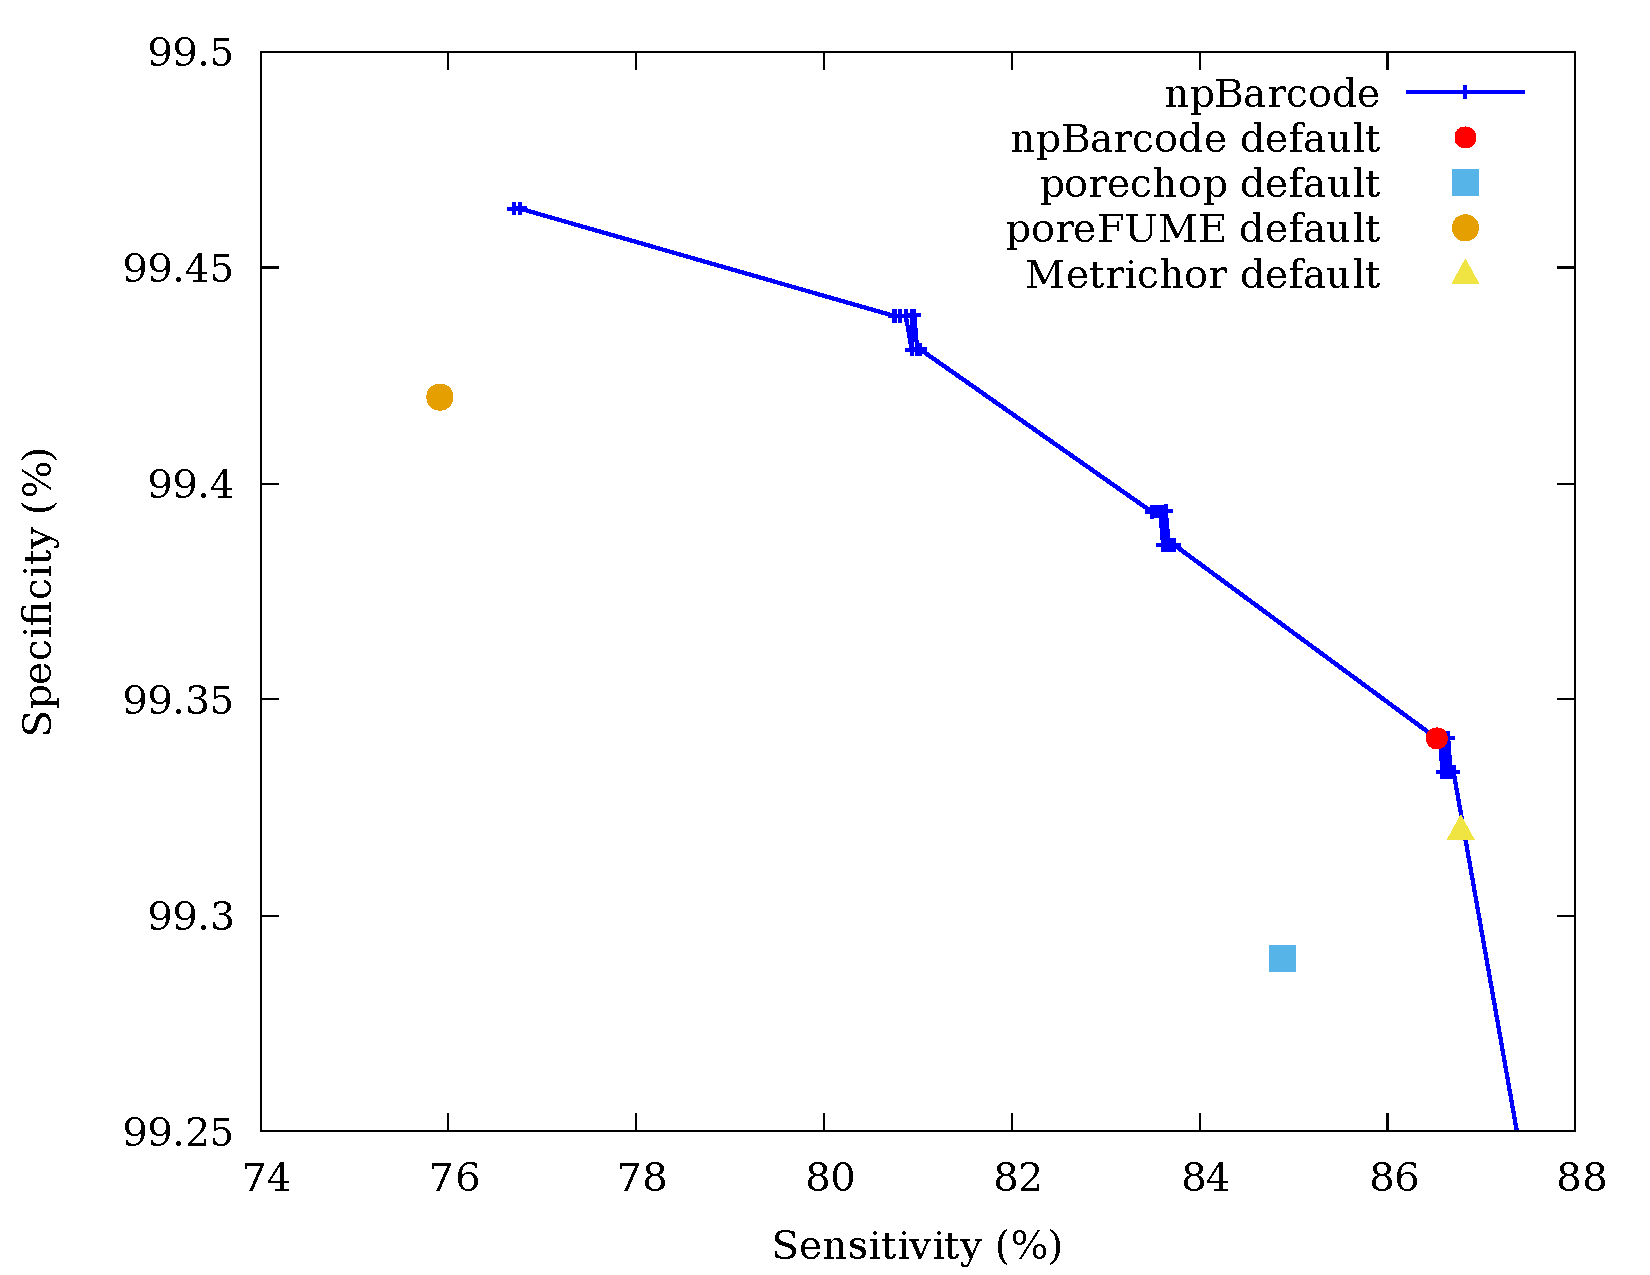
\includegraphics[width=0.6\textwidth]{images/roc.pdf}}
\caption{Plot of sensitivity versus specificity of \npbarcode{} compared
with existing tools.}
\label{fig:sen}
\end{figure}

We barcoded and sequenced 8 different bacterial strains on a single MinION R9.4 flow cell using the Oxford Nanopore Technology's 2D native barcoding kit (SQK-LSK208 + EXP-NDB002). Another run with PCR barcoding kit for 3 libraries is not discussed here as part of a different study, but its result is included in Appendix Figure~\ref{supp_fig:npbarcode_pcr}.

The pool consisted of one gram positive isolate (\emph{Staphylococcus aureus}) and seven gram negative isolates (four \emph{Klebsiella pneumoniae}, one \emph{Klebsiella quasipneumoniae}, one \emph{Pseudomonas aeruginosa} and one \emph{Acinetobacter baumannii}).
In order to establish a ground truth benchmark for  comparison of different de-multiplexing tools, we aligned the sequence reads of the eight samples to their respective assemblies to identify the original source of the reads. 
Due to the high level of similarity among the gram negative isolates, we could only obtain the confident assignment of reads to the \emph{S. aureus}, a gram positive strain, versus the other gram negative strains. 
Hence, we set up the comparison framework as the accuracy of the tool detecting the barcode associated with the \emph{S. aureus} sample. For an exhaustive benchmark for each of every strains included, ones can assess Appendix Figure~\ref{supp_fig:comparison}.

Figure~\ref{fig:sen} presents the sensitivity and specificity of \npbarcode{} with differing parameters. We also obtained the results from Metrichor, porechop and poreFume with their default parameter settings. 
Statistics of all tools with their automatic settings is depicted in details in Appendix Table~\ref{supp_tab:sensitivity}.
We found that \npbarcode{} performed comparably with Metrichor and was marginally more accurate than the competitive porechop and poreFUME.


\subsubsection{Real-time scaffolding pipeline for multiple samples}

\begin{figure}[!hpb]
\centering
\subfloat[\emph{K. pneumoniae} isolate 1]{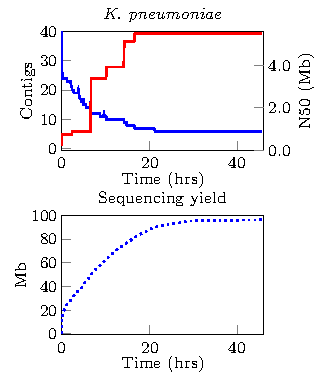
\includegraphics[width=0.30\textwidth]{images/s092.pdf}}%
\subfloat[\emph{K. pneumoniae} isolate 2]{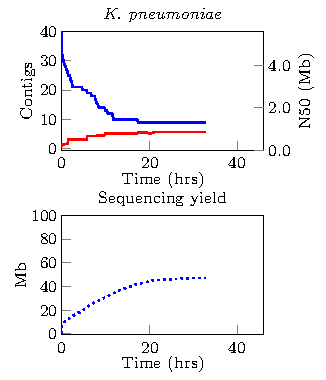
\includegraphics[width=0.30\textwidth]{images/s133.pdf}}%
\subfloat[\emph{K. pneumoniae} isolate 3]{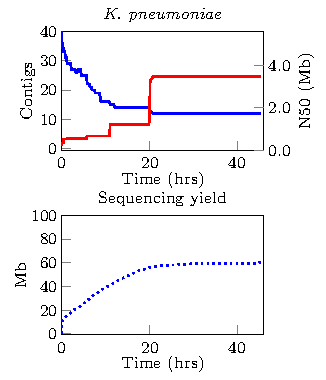
\includegraphics[width=0.30\textwidth]{images/s096.pdf}}%
\\
\subfloat[\emph{K. pneumoniae} isolate 4]{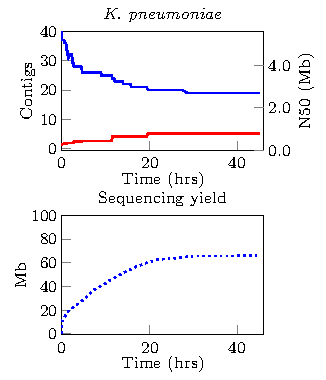
\includegraphics[width=0.30\textwidth]{images/s106.pdf}}%
%\hfill
\subfloat[\emph{K. quasipneumoniae} isolate]{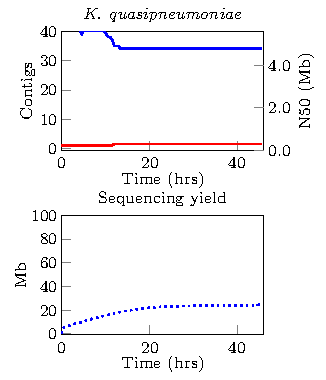
\includegraphics[width=0.30\textwidth]{images/s132.pdf}}%
%\hfill
\subfloat[\emph{A. baumannii} isolate]{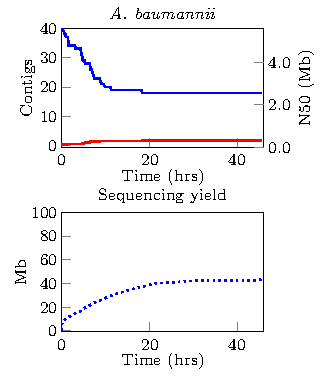
\includegraphics[width=0.30\textwidth]{images/s093.pdf}}%
%\hfill
\\
\subfloat[\emph{P. aeruginosa} isolate]{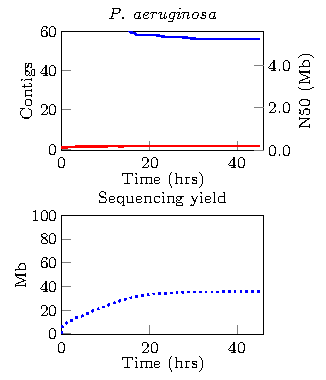
\includegraphics[width=0.30\textwidth]{images/s101.pdf}}%
%\hfill
\caption[A combining pipeline of \npreader{}, \npbarcode{} and \npscarf{} with ONT Native Barcoding Kit]{Result for running a combining pipeline of \npreader{}, \npbarcode{} and \npscarf{} with ONT Native Barcoding Kit in order to scaffold genomes of 7 gram-negative samples in real-time. For each sample, the upper plot shows number of contigs (blue) and N50 (red) while the lower graph presents data yield (bases) for that particular demultiplexed sample over time.}
\label{fig:scaffold}
\end{figure}

As part of the experiment, we also integrated \npbarcode{} into a streaming analysis
pipeline where we scaffolded genome assemblies in real-time. Prior to the MinION run, we sequenced the seven gram negative samples with Illumina technology and used \spades{}~\cite{BankevichNA2012} to assemble them into
more than 100 contigs each. 
The \emph{S. aureus} sample was used as a control sample during 
demultiplexing, and was not used for scaffolding.
As soon as a sequence read was generated, it was base-called, demultiplexed and
streamed into the appropriate instance of \npscarf{}~\cite{Cao2017scaffolding} 
for scaffolding. This
pipeline allowed us to simultaneously scaffold all seven bacterial samples while
the sequencing was still in progress (Figure~\ref{fig:scaffold}). We were able 
to complete the genome of one \kp{} isolate after 16 hours of
sequencing and with about $80$Mbp of nanopore sequencing data. While the genomes of 
the other six isolates were not completed due to their low proportions in the 
pooled sample, and the less than ideal yield of the run, they were significantly
improved over time with nanopore long reads.

\subsubsection{Graphical user interface}

\begin{figure}[ht]
\centerline{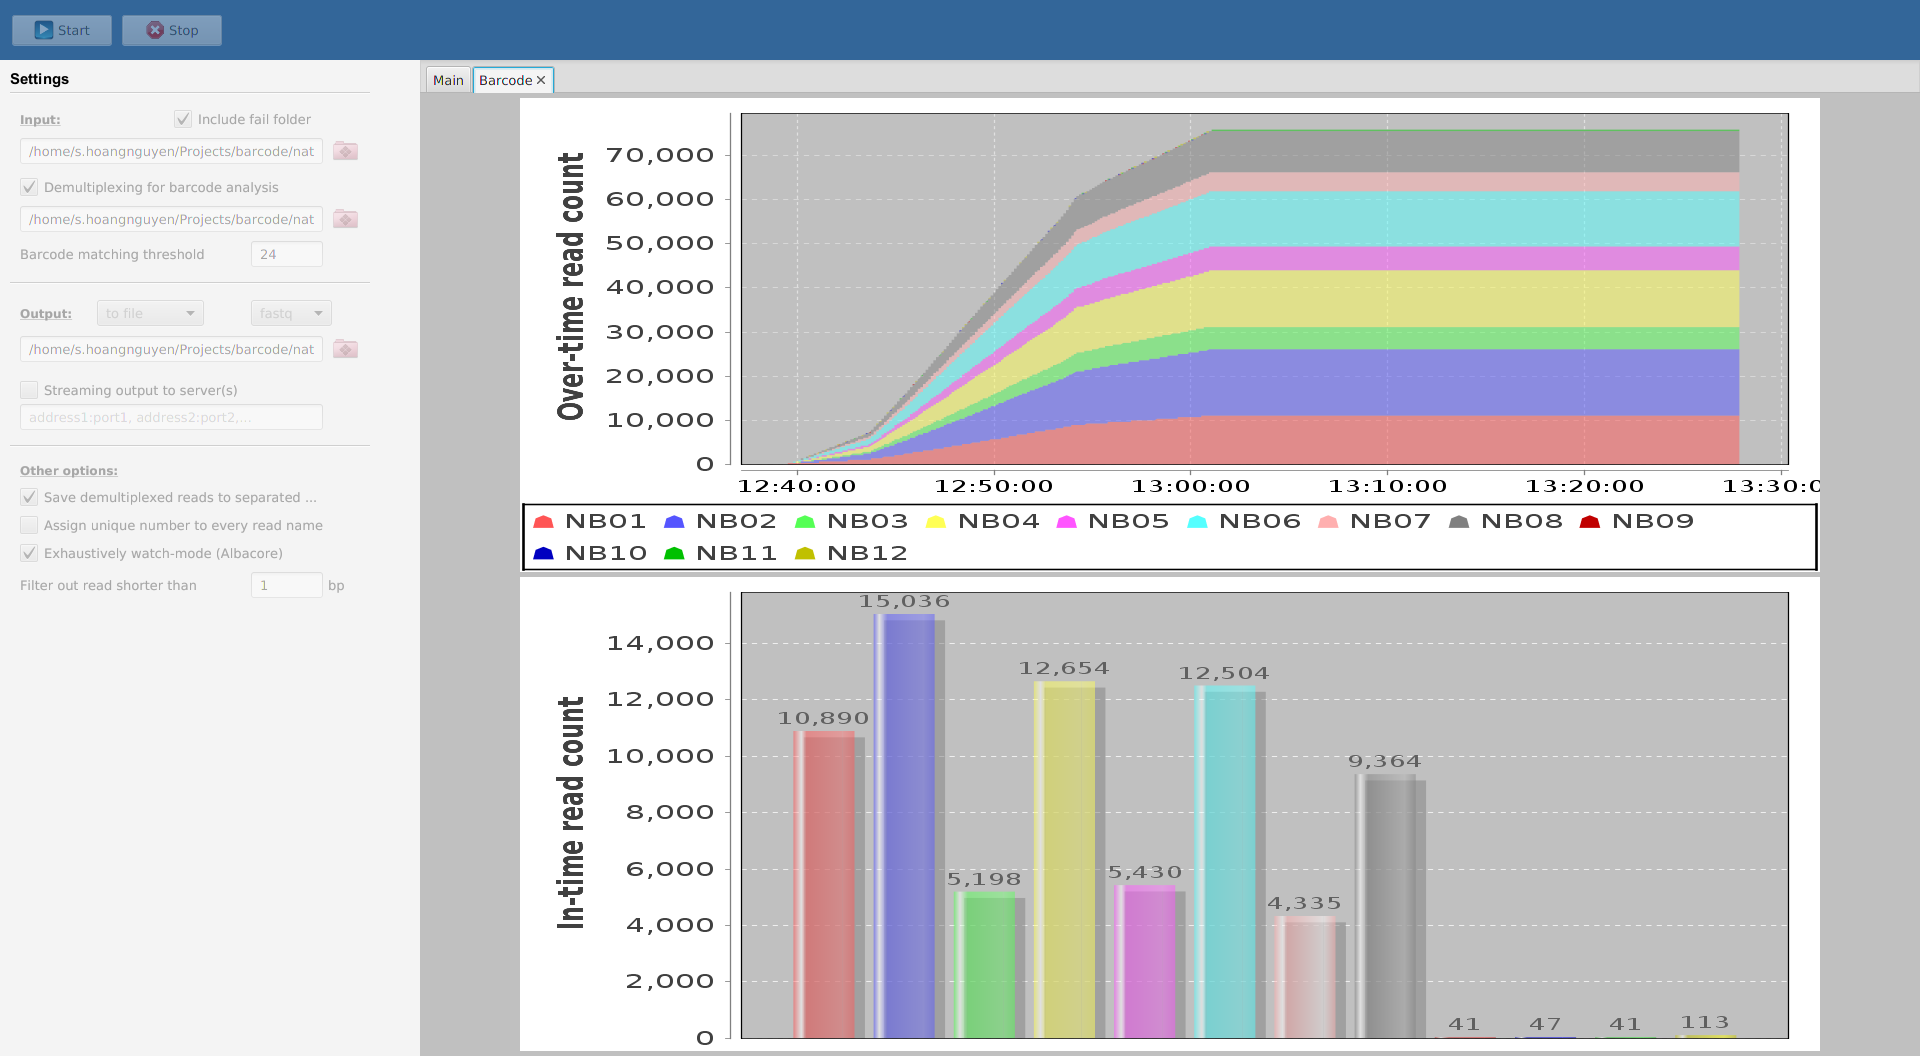
\includegraphics[width=0.9\textwidth]{images/native2.png}}
\caption{Graphical User Interface of npBarcode integrated in npReader. The 
result shown is for the a MinION run using Native barcoding kit on 8 libraries.}
\label{fig:gui_npbarcode}
\end{figure}
\npbarcode{} is also integrated into \npreader{}'s graphical user interface. This allows users to monitor the amount of sequencing data for each pooled sample
in real-time. When required, \npreader{} provides a view showing read-count per bin 
in a real-time fashion. This view provides two plots that can depict the progress 
in an over-time and in-time manner, respectively. The top graph shows a more general progress viewing by showing the read count of the whole process 
while the lower graph figures the exact number of binned reads at a particular 
time point. An example of the visualization is shown in Figure~\ref{fig:gui_npbarcode}. 
Overall it reflects the 
demultiplex functioning appropriately with the majority of reads falling in the 
bins corresponding to the samples used for the barcode sequencing. Only an 
negligible  amount of reads are mis-classified into unrelated bins.

\subsection{Methods}
\subsubsection{Bacterial cultures and DNA extraction}
Bacterial strains include \emph{Streptococcus pneumoniae} from the American Type Culture Collection (ATCC 700677) and clinical isolates from Hygeia General Hospital, Athens, Greece or Instituto Dante Pazzanese de Cardiologia, Brazil~\cite{Miranda2018}. Clinical isolates comprise of four \emph{Klebsiella pneumoniae} (3\_GR\_13, 5\_GR\_13, 11\_BR\_13, 22\_GR\_12), \emph{Klebsiella quasipneumoniae} (21\_GR\_13), \emph{Acinetobacter baumannii} (source: Hygeia General Hospital, 2013) and \emph{Pseudomonas aeruginosa} (source: Hygeia General Hospital, 2013). It is worth noting that the sample identifiers are re-assigned for convenient as shown in Table~\ref{supp_tab:sample} which emphasize on the gram stain of the bacteria: GP for gram positive and GN for gram negative.
Bacterial cultures were supplied as stabs/slants or on agar, grown in nutrient broth or brain heart infusion broth, glycerol stocks were made to $20 \%$ (v/v) glycerol and stored at $−80^o$C.

For DNA extractions, glycerol stocks were struck out on either nutrient agar or tryptic soy agar with $5\%$ defibrinated sheep blood to isolate single colonies. Strains were grown overnight at $37^o$ shaking at 220 rpm and DNA subsequently extracted from this inoculum. DNA was isolated using the DNeasy Blood and Tissue Kit (Qiagen) with the additional enzymatic lysis buffer pre-treatment as per the manufacturer’s instructions. DNA was quantified with Qubit3.0 (ThermoFisher Scientific).
\subsubsection{Illumina sequencing and assembly}
One nanogram of DNA was used for the Nextera XT (Illumina) library preparation as per the manufacturer’s instructions and quality was evaluated via a 2100 Bioanalyzer (Agilent Technologies). Libraries were sequenced on an Illumina MiSeq (300 bp paired-end reads) with $>$100X coverage per sample.

The raw reads from each data set were processed by  $\mathtt{Trimmomatic}$~\cite{BolgerLU2014} version 0.36 to remove adapter sequences and attain paired reads only. After that, \spades{} 3.10.1 was used to generate short-read assembly consisting of high quality contigs.
\subsubsection{MinION barcode sequencing}
The same DNA extract from the Illumina sequencing run was used for Nanopore sequencing. The library preparation was done following the 2D native barcoding kit (SQK-LSK208 + EXP-NDB002) with the input between 900 to 1500 nanograms of DNA for each sample as in Table~\ref{supp_tab:sample}. 
The samples were pooled in equimolar concentrations and 15.75ng was loaded into a R9.4 FLOMIN106 flow cell. After 20 hours the flow cell was topped up with 6$\mu$L of library.

The sequencing run was stopped after 43 hours and generated 65,029 reads and 331,329,280 events. The reads were basecalled with settings: 2D Basecalling plus Barcoding for FLO-MIN106 250bps - v1.125.
\subsubsection{Comparative metrics}
We conduct a sensitivity/specificity test on the ability to identify the only gram positive bacterial \emph{S.~aureus} of the interested binning algorithms. The rationale stems from the fact that it has the most distinctive genome compare to the others (as shown in Appendix~\tab{supp_tab:dnadiff}), therefore it would account for the least probability of having ambiguous alignments. Statistics are generated as: the number of indeed aligned reads from the bin \emph{S.~aureus} (true positive); number of unaligned reads in the bin (false positive); number of aligned (false negative) and unaligned (true negative) reads from outside the bin. Sensitivity and specificity are then calculated by following equations:
$
	\mtt{sensitivity} = \frac{\mtt{TP}}{\mtt{TP+FN}} ;~
    \mtt{specificity} = \frac{\mtt{TN}}{\mtt{TN+FP}}
$
where $\mtt{TP}$, $\mtt{FN}$, $\mtt{TN}$ and $\mtt{FP}$ stand for true positive, false negative, true negative and false positive respectively.

\subsubsection{Software UI design}
We provide both command line and graphical user interface for nanopore barcode sequencing. While the former is flexible and convenient to those who want to integrate downstream analysis directly from demutiplexed results, the latter offers a simpler maneuver and better visualization.

From terminal, one can invoke either $\mathtt{jsa.np.npreader}$ with barcode input sequences specified, or dedicated $\mathtt{jsa.np.barcode}$ module which requires an executable script for downstream analysis. 

On the other hand, users can type $\mathtt{jsa.np.npreader -gui}$ to have a user-friendly demultiplex running, especially for streaming-mode as the sequencing is still ongoing.
Beside the traditional \npreader{}'s window, whenever having a demultiplex phase involved, there is an additional tab view showing binned read-count in a real-time fashion. This view provides 2 plots that can depict the progress in an over-time and in-time manner respectively. The top graph would offer more general progress viewing by showing the read count of the whole process while the lower graph figures the number of binned reads in more detail at a particular time point.

\subsubsection{Real-time analysis setup}
% how to setup a streaming pipeline...
Users can implement a streaming pipeline that consumes demultiplexed output from \npbarcode{} in two ways. 
The first method is simply watching the content of the appending output files and explicitly pipe them to appropriate downstream processes, \EG{} by using $\mathtt{tail -f}$.
In order to do this, ones initially need to tell \npbarcode{} to output the demultiplexed sequences into different files to read from.

Another way, which has been used in this study, is to provide a script for downstream scenario to \npbarcode{} and let it handle implicitly. This approach will reduce the I/O operations and disk space required for the analysis. For example, in order to invoke \npscarf{} to scaffold multiple samples at the same time using barcoded sequences, we stream the base-called sequence to \npbarcode{} command line via the inter-process communication (Linux pipe) or network channels (Java sockets) protocol \cite{CaoGE2015} and provide it a script ($\mathit{script.sh}$) to invoke \npscarf{}. An example of such bash script is given in Appendix List \ref{lst:script}.

$\mathtt{<data \: stream>}~|~\mathtt{jsa.np.barcode} \ \mathtt{-seq} \ \mathit{-} \ \mathtt{-bc} \ \mathit{barcode.fasta} \ \mathtt{-sc} \ \mathit{script.sh}$

where $\mathtt{<data \: stream>}$ is the input stream and $\mathit{barcode.fasta}$ is the file containing the actual barcode sequences that have been used.
From an appending base-called output file, the stream can be achieved by a monitoring command, \EG{} $\mathtt{tail}\ \text{-}\mathtt{f}$ (for a local mounted file system) or by using socket communication utility, \EG{} $\mathtt{jsa.util.streamServer}$ and $\mathtt{jsa.util.streamClient}$ from Japsa package.
Refer to \href{http://japsa.readthedocs.org/en/latest/index.html}{Japsa documentation} for more details.

\subsection{Conclusion}

We have described \npbarcode{}, a tool supporting real-time demultiplex of nanopore sequencing data. 
Depending on requirements, users can choose to run the dedicated demultiplexer from command line or using it as part of \npreader's graphical user interface. 
The tool provides practitioners a flexible option to monitor a barcoded sequencing run as well as to integrate pooled sequencing into a streaming analysis pipeline.

Shortly after the manifestation of open-sourced demultiplexers such as \npbarcode{}, Albacore and new (commercial) version of Metrichor have been offered to the community that integrate direct FASTQ output as well as demultiplex option. The overlapping functionality lead to the retirement of \npreader{} and \npbarcode{} maintenance, however, they are still applicable for the use cases that demands flexible control and customization from end users. The code is made available and free via \href{https://github.com/mdcao/japsa}{Japsa} package.  

In the next section, we adopt a combination of in-house tools and other open-source software for another assembly use case in order to comprehend the resistance gene profile of several Extensively Drug-Resistant (XDR) \kp{} strains using MinION sequencing.

\section{Assembly of multiple XDR strains for \emph{Klebsiella~pneumoniae}} 
The following detail is extracted from a submitted publication with permission from its corresponding authors.
As part of this thesis, I only report my major contributions in the publication, \IE{} genome assembly and associated computational analysis on the DNA barcode sequencing data. 

In this section, a combined application of \npscarf{} with other assemblers is implemented to generate the final assembly of interests. Such practice can demonstrate in depth the performances of each method and at the same time, provide a consensus approach for a \emph{de novo} reference-free assembly.
This use case also highlights the ability of long-read assembly in discerning the location of acquired resistance in the whole genomes of XDR bacterial strains, especially on the identified plasmid(s).
\subsection{Introduction}
The bacterial samples exclusively subjected to this research conduct were \emph{Klebsiella pneumoniae}, a species known as one of the prominent pathogens found in health care facilities.
As a matter of fact, \kp{} is vastly responsible for the risks of \emph{nosocomial} infections (caused by transmission of germs within hospital environment) with mortality rate has been observed as high as 50\%~\cite{Martin2018M1,Magill2014M2,Kalanuria2014M3,Talha2009M4,Podschun1998M5}. 
More importantly, the treatment options are becoming limited as the bacteria is developing its resistance to the available antibiotics, including carbapenems, fosfomycin, tigecycline and polymyxins~\cite{Karaiskos2014M7}. As shown by current evidence, plasmids are the primary source of resitance genes~\cite{HudsonBMW2014} of the \emph{superbugs} and are irrepressibly disseminating them to other strains, accounting for the rapid global dissemination of resistance~\cite{Martin2018M1,Navon2017M6}. 
More severely, pandrug-resistant (PDR) \kp{} strains have been reported as resistant to all commercially available antibiotics~\cite{Chen2017M8,Zowawi2015} at the moment.

The shortcoming for a robust detection methodology to accurately assess bacterial infections, the resistance profile in particular, has been considered as one factor accounting for the exhibition of antibiotic resistance~\cite{sommer2017M10}.
In light of antimicrobial therapy, this drawback gave rise to the unnecessary applications of antibiotics for viral infections and ineffective antibiotics being administered for resistant infections. 
Rapid sequencing has been proposed as a way to determine PDR profiles, including approaches which utilize high accuracy short reads, as well as those which utilize real-time single molecule sequencing. 
In particular, MinION is a portable single-molecule sequencer which can sequence long fragments of DNA and stream the sequence data for further data processing in real-time to detect the presence of bacterial species and acquired resistance genes~\cite{Gardy2018M11, Lemon2017M15,Votintseva2017M16,CaoGE2016,QuickAC2015}. 

Moreover, the long reads coupled with the ability to multiplex samples has immensely aided with the assembly of bacterial genomes~\cite{Nguyen2017barcode,Wick2017M12,Li2018M13,George2017M14}. 
This capability allows for the rapid determination of whether resistance is residing on the chromosome or plasmid(s). 
Of particular interest are high levels of resistance encoded on plasmids, as these genes can rapidly be transferred throughout the bacterial population via horizontal gene transfer.

\subsection{Data description}
MinION sequencing and associated computational analysis were conducted to interrogate the resistance profile in the whole genomes of four XDR clinical \kp{} strains. These isolates had been previously sequenced by Illumina platform and undergone antimicrobial susceptibility testing.
Three of them, namely 1\_GR\_13, 2\_GR\_12 and 16\_GR\_13, exhibited resistance to all 24 classes or combinations of antibiotics tested, including the `last resort' polymyxin. Accordingly, there were high abundance of antibiotic resistance genes found in these samples' genome ($\geq 26$)~\cite{Miranda2018}. 
Another polymyxin-susceptible XDR isolate, 20\_GR\_12, was included for comparative studying purpose.
%%%Table: sequencing stats
\begin{table}[!hpt]
\centering
\caption{Sequencing data statistics for each \kp{} strains.}
\label{tab:assers_stats}
\begin{tabular}{|c|c|r|r|r|r|r|}
\hline
\multirow{2}{*}{\textbf{Strain}} & \multirow{2}{*}{\textbf{Lineage}} & \multicolumn{2}{c|}{\textbf{Illumina}}                                     & \multicolumn{3}{c|}{\textbf{Nanopore}}                                                            \\ \cline{3-7} 
                                 &                                   & \multicolumn{1}{c|}{\textbf{Coverage(X)}} & \multicolumn{1}{c|}{\textbf{N50$^a$}} & \multicolumn{1}{c|}{\textbf{Coverage(X)}} & \multicolumn{1}{c|}{\textbf{N50$^b$}} & \textbf{Time(mins)} \\ \hline
1\_GR\_13                        & ST147                             & 63                                     & 242,838                           & 215                                    & 8,712                             & 1,279                \\ \hline
2\_GR\_12                        & ST258                             & 158                                    & 196,706                           & 67                                     & 5,251                             & 2,468                \\ \hline
16\_GR\_13                       & ST11                              & 123                                    & 203,529                           & 101                                    & 5,012                             & 1,277                \\ \hline
20\_GR\_12                       & ST258                             & 262                                    & 256,217                           & 115                                    & 10,151                            & 1,277                \\ \hline

\multicolumn{7}{l}{\small{$^a$ of the Illumina assembly contigs.}}\\
\multicolumn{7}{l}{\small{$^b$ of the raw Nanopore sequences.}}
\end{tabular}
\end{table}

The WGS sequencing yield and length statistics for each sample are shown in Table~\ref{tab:assers_stats}. 
Illumina paired-end data was assembled by \spades{} v3.10.1 \cite{BankevichNA2012}. The fact of having more than 60-folds coverage for each sample assures the high quality of the short-read assembly.
The Rapid Barcoding Sequencing was used for a mixture of 1\_GR\_13, 16\_GR\_13 and 20\_GR\_12 and the base-called data were demultiplexed by \npbarcode{}. Isolate 2\_GR\_12, due to potential carbonhydrate contamination, has been prepared separately and subjected to another MinION run using Rapid Sequencing Kit. As shown in the table, this sample has the least coverage of Nanopore data despite of the longest sequencing time. The low N50 values of 2\_GR\_12 and 16\_GR\_13 ($\simeq 5$Kbp) may introduce difficulties in completing their genomes using hybrid approaches, however, the abundance of long-read data from the latter would increase the chance of having appropriate bridges over the repetitive elements.
\subsection{\emph{De novo} assembly with multiple approaches}
In order to have the assembly of high confidence without any reference genomes, multiple prominent approaches were applied to the data set. 
The real-time assembly is not reported here as exhaustive operations of MinION flow cells were established in expectations to obtain as much data as possible, not to mention \npscarf{} is the only tool supporting the streaming mode. Instead, only the final assembly were of interest. 
After having results from different assemblers, an alignment-based comparative interrogation was conducted to investigate the completeness and quality of each contigs in relations with its corresponding counterparts.
By doing so, the consensus sequence can be determined as the best candidate among all.

% \begin{landscape}
% \begin{table}[!hpt]
% \centering
% \footnotesize
% \caption[Genome assembly of multiple approaches.]{Genome assembly of multiple approaches. Output identifies circular sequences in \textbf{bold} and in brackets plasmid replicons if present.}
% \label{tab:assers}
% \begin{tabular}{|c|p{5cm}|p{5cm}|p{5cm}|p{5cm}|}
% \hline
% \multirow{2}{*}{Strain} & \multicolumn{4}{c|}{Assembly method}\\ \cline{2-5} 
%                         & \multicolumn{1}{c|}{npScarf}  & \multicolumn{1}{c|}{Unicycler}    & \multicolumn{1}{c|}{Canu} & \multicolumn{1}{c|}{minasm+Racon} \\ \hline
% 1\_GR\_13               & \textbf{5,289,533 (IncFIB)}; \textbf{193,063 (IncA/C2)}; \underline{\textbf{168,873 (IncFIB, IncFII)}}; 61,039; \textbf{53,489(IncR, IncN)}; 55,020; \textbf{6,457}              & \underline{\textbf{5,181,675}}; \underline{\textbf{192,771(IncA/C2)}}; 159,172 (IncFIB, IncFII); \underline{\textbf{108,879 (IncFIB)}}; \underline{\textbf{55,018}}; \underline{\textbf{53,495 (IncR, IncN)}};                                                        & \textbf{5,073,727}; \textbf{226,704 (IncA/C2)}; \textbf{184,820 (IncFIB,IncFII)}; \textbf{136,154 (IncFIB)}; 100,186; \textbf{82,924 (IncR,IncN)}; 54,495       & \textbf{5,167,584}; \textbf{192,237 (IncA/C2)}; \textbf{168,292 (IncFIB, IncFII)}; \textbf{108,582 (IncFIB)}; \textbf{53,325 (IncR, IncN)}                                \\ \hline
% 2\_GR\_12               & \underline{\textbf{5,466,424}}; 457,649 (IncFIB, IncA/C2, IncFII); 60,365 (IncFII); 42,041 (IncX3); 32,458; 21,300; \underline{\textbf{13,841 (ColRNAI)}}; 12,226 & 3,743,268; 1,694,231; \underline{175,636 (IncA/C2)}; 152,644 (IncFIB, IncFII); \underline{95,481 (IncFIB)}; \underline{\textbf{43,380 (IncX3)}}; 28,913; 26,127;16,315; 16,781 (IncFII); \underline{\textbf{13,841 (ColRNAI)}} & 5,440,093; 392,198 (IncFIB,IncA/C2,IncFII); 122,463 (IncFIB,IncFII); 57,534 (IncX3); 26,891 (ColRNAI)              & 3,769,033; 1,696,038; 204,124 (IncA/C2); 179,356 (IncFIB, IncFII); 158,561 (IncFIB); \textbf{43,085 (IncX3)}; 13,400 (ColRNAI); 2,250 \\ \hline
% 16\_GR\_13              & \underline{\textbf{5,426,917}}; \textbf{186,908 (IncFIB,IncFII)}; \textbf{154,971 (IncA/C2)}; \textbf{63,588 (IncL/M)}; 37,608; 35,578; \textbf{5,225}; 4,426 (ColRNAI); \textbf{3,703}   & \textbf{5,426,765}; \underline{\textbf{187,670 (IncFIB,IncFII)}}; \underline{\textbf{155,161 (IncA/C2)}}; \underline{\textbf{63,589 (IncL/M)}}; \underline{\textbf{5,234}}; \underline{\textbf{4,940 (ColRNAI)}}; 2,156 (ColRNAI)                                              & \textbf{5,400,611}; \textbf{199,904 (IncFIB,IncFII)}; \textbf{180,542 (IncA/C2)}; \textbf{83,467 (IncL/M)}; 14,853; 11.623; 9,308; 9,423; 7,568; 7,089 & \textbf{5,410,256}; \textbf{186,950 (IncFIB,IncFII)}; \textbf{154,635 (IncA/C2)}; \textbf{63,299 (IncL/M)}; 5,100; 4,900                                         \\ \hline
% 20\_GR\_12              & \textbf{5,391,578}; \textbf{163,468 (IncFIB,IncFII)}; \textbf{50,940 (IncN)}; 50,856 (IncX3); 12,578 (ColRNAI)                                     & \underline{\textbf{5,395,894}}; \underline{\textbf{170,467 (IncFIB,IncFII)}}; \underline{\textbf{50,979 (IncN)}}; \underline{\textbf{43,380 (IncX3)}}; \underline{\textbf{13,841 (ColRNAI)}}; 4,645                                                                   & 5,342,491; \textbf{192,947 (IncFIB,IncFII)}; 74,844 (IncX3); 72,588 (IncN); 25,624 (ColRNAI)                                & \textbf{5,380,057}; \textbf{169,880 (IncFIB,IncFII)}; \textbf{50,636 (IncN)}; \textbf{43,157 (IncX3)}; 13,600 (ColRNAI)                                          \\ \hline
% \end{tabular}
% \end{table}
% \end{landscape}

\begin{landscape}
\begin{table}[!hpt]
\centering
\small
\caption[Genome assembly results using multiple approaches.]{Contigs in the genome assembly results of 4 \kp{} isolates using multiple approaches. Output identifies circular sequences in \textbf{bold} and \underline{underlined} if chosen for the final assembly.}
\label{tab:assers}
\begin{tabular}{|c|p{4cm}|p{4cm}|p{4cm}|p{4cm}|}
\hline
\multirow{2}{*}{Isolate} & \multicolumn{4}{c|}{Assembly method}\\ \cline{2-5} 
                        & \multicolumn{1}{c|}{npScarf}  & \multicolumn{1}{c|}{Unicycler}    & \multicolumn{1}{c|}{Canu} & \multicolumn{1}{c|}{minasm+Racon} \\ \hline
1\_GR\_13               & \textbf{5,289,533}; \textbf{193,063}; \underline{\textbf{168,873}}; 61,039; \textbf{53,489}; 55,020; \textbf{6,457}              & \underline{\textbf{5,181,675}}; \underline{\textbf{192,771}}; 159,172; \underline{\textbf{108,879}}; \underline{\textbf{55,018}}; \underline{\textbf{53,495}};                                                        & \textbf{5,073,727}; \textbf{226,704}; \textbf{184,820}; \textbf{136,154}; 100,186; \textbf{82,924 }; 54,495       & \textbf{5,167,584}; \textbf{192,237}; \textbf{168,292}; \textbf{108,582}; \textbf{53,325}                                \\ \hline
2\_GR\_12               & \underline{\textbf{5,466,424}}; 457,649; 60,365; 42,041; 32,458; 21,300; \underline{\textbf{13,841}}; 12,226 & 3,743,268; 1,694,231; \underline{175,636}; 152,644; \underline{95,481}; \underline{\textbf{43,380}}; 28,913; 26,127;16,315; 16,781; \underline{\textbf{13,841}} & 5,440,093; 392,198; 122,463; 57,534; 26,891   & 3,769,033; 1,696,038; 204,124; 179,356; 158,561; \textbf{43,085}; 13,400; 2,250 \\ \hline
16\_GR\_13              & \underline{\textbf{5,426,917}}; \textbf{186,908}; \textbf{154,971}; \textbf{63,588}; 37,608; 35,578; \textbf{5,225}; 4,426; \textbf{3,703}   & \textbf{5,426,765}; \underline{\textbf{187,670}}; \underline{\textbf{155,161}}; \underline{\textbf{63,589}}; \underline{\textbf{5,234}}; \underline{\textbf{4,940}}; 2,156  & \textbf{5,400,611}; \textbf{199,904}; \textbf{180,542}; \textbf{83,467}; 14,853; 11.623; 9,308; 9,423; 7,568; 7,089 & \textbf{5,410,256}; \textbf{186,950}; \textbf{154,635}; \textbf{63,299}; 5,100; 4,900  \\ \hline
20\_GR\_12              & \textbf{5,391,578}; \textbf{163,468}; \textbf{50,940}; 50,856; 12,578  & \underline{\textbf{5,395,894}}; \underline{\textbf{170,467}}; \underline{\textbf{50,979}}; \underline{\textbf{43,380}}; \underline{\textbf{13,841}}; 4,645     & 5,342,491; \textbf{192,947}; 74,844; 72,588; 25,624    & \textbf{5,380,057}; \textbf{169,880}; \textbf{50,636}; \textbf{43,157}; 13,600  \\ \hline
\end{tabular}
\end{table}
\end{landscape}

In particular, the enforced hybrid assemblers included \npscarf{} and \unicycler{} v0.3.1 \cite{Wick2017unicycler}. Assemblers using only ONT reads were \canu{} v1.5 \cite{Koren2017canu} (excluding read shorter than 500bp) and a combination pipeline of \miniasm{} v0.2-r-168-dirty, \minimap{} v2.1-r311; \racon{}~(git commit 834442) were used in both cases to polish the assemblies afterward~\cite{Vaser2017racon}. Consensus sequences were determined among all obtained assemblies manually using visualization from $\mathtt{Mauve}$ \cite{Darling2011mauve} snapshot\_2015-02-13. 
From which, potential bridging differences between candidates were further investigated by alignments with Illumina paired-end data on $\mathtt{IGV}$ 2.3 \cite{Robinson2011IGV,Thorvaldsdottir2013IGV}. 

The output from each assembly method is reported in Table~\ref{tab:assers}. 
Overall, \unicycler{} returned most accurate results and as the consequence, a majority of the final assembly were composed from its output contigs. The high quality achieved thanks to the application of the optimized assembly graph in \unicycler{}'s hybrid assembly module, as well as comprehensive post-processing steps carried out on the draft sequences subsequently~\cite{Wick2017unicycler}. 
\npscarf{}, on the other hand, can generate longer contigs but the results are more susceptible to mis-assemblies. The algorithm, which is independent on the assembly graph, can bridge two nodes that lack connections in the graph, but at the same time, is more prone to erroneous alignments. 
The two remaining methods, even though with polishing step, produced inferior results but would give additional information for the ultimate backbones of the assembly.

Amongst four data sets, 2\_GR\_12 shows most fragmented assembly as the shorter reads could not resolve all repeats. For this sample, only \npscarf{} and \canu{} can successfully assemble the chromosomal sequence as the longest contig of length $\simeq 5.4$Mbp. Two other circular sequences were reports as complete plasmid DNA from \unicycler{}. In addition, there were 3 unfinished (linear) sequences in the final assembly for this sample, corresponding to 5 fragmented contigs from \unicycler{}. Another longest contig found by \npscarf{} belonged to 16\_GR\_13 data set (5,426,917bp). \unicycler{} reported very close circular sequence (5,426,765bp) with equivalent quality but hosting less genes than the former thus was not selected in this case. %Other than that, its reported contigs were mostly designated as the consensus sequences in the final result.

\subsection{AMR analysis on the final assembly}

\begin{landscape}
\begin{table}[!ht]
\centering
\scriptsize
\caption{Final assembly of XDR \kp{} isolates and location of antibiotic resistance genes.}
\label{tab:assers_final}
\begin{tabular}{|l|l|r|c|p{12cm}|}
\hline
\multirow{2}{*}{\small Isolate}  & \multirow{2}{*}{\small Contig$^a$}   & {\small Length$^b$} & {\small Abundance} & \multirow{2}{*}{\small Resistance Genes$^c$}\\
 & & (bp) & (X) & \\ \hline \hline
\multirow{6}{*}{1\_GR\_13}  & C                           & \textbf{5,181,675}     & 1        & blaSHV-11, fosA, oqxA, oqxB                                                                                                                \\ \cline{2-5} 
                            & P: IncA/C2                  & \textbf{192,771}      & 1.95     & aadA1, ant(2'')-Ia, aph(6)-Id, ARR-2, blaOXA-10, blaTEM-1B, blaVEB-1, cmlA1, dfrA14, dfrA23, rmtB, strA, sul1, sul2, tet(A), tet(G)        \\ \cline{2-5} 
                            & P: IncFIB$_{pKpn3}$, IncFII$_{pKP91}$ & \textbf{168,873}      & 2        & aadA24, aph(3')-Ia, aph(6)-Id, dfrA1, dfrA14, strA                                                                                         \\ \cline{2-5} 
                            & P: IncFIB$_{pKPHS1}$             & \textbf{108,879}      & 1.53     & -                                                                                                                                          \\ \cline{2-5} 
                            & -                           & \textbf{55,018}       & 14.10    & -                                                                                                                                          \\ \cline{2-5} 
                            & P: IncR, IncN               & \textbf{53,495}       & 2.36     & aadA24, aph(3')-Ia, aph(6)-Id, blaVIM-27, dfrA1,mph(A), strA, sul1                                                                         \\ \hline \hline
\multirow{6}{*}{2\_GR\_12}  & C                           & \textbf{5,466,424}     & 1        & blaSHV-11, fosA, oqxA, oqxB                                                                                                                \\ \cline{2-5} 
                            & P: IncFIB$_{pKpn3}$, IncFIIK     & 197,872      & 1.3      & aadA2, aph(3')-Ia, catA1, dfrA12, mph(A), sul1                                                                                             \\ \cline{2-5} 
                            & P: IncA/C2                  & 175,636      & 1.49     & aadA1, ant(2'')-Ia, aph(3'')-Ib, aph(6)-Id, ARR-2, blaOXA-10, blaTEM-1A, blaVEB-1, cmlA1, dfrA14, dfrA23, rmtB, sul1, sul2, tet(A), tet(G) \\ \cline{2-5} 
                            & P: IncFIB$_{pQil}$               & 95,481       & 1.61     & blaKPC-2, blaOXA-9, blaTEM-1A                                                                                                              \\ \cline{2-5} 
                            & P: IncX3                    & \textbf{43,380}       & 1.91     & blaSHV-12                                                                                                                                  \\ \cline{2-5} 
                            & P: ColRNAI                  & \textbf{13,841}       & 4        & aac(6')-Ib, aac(6')Ib-cr                                                                                                                   \\ \hline \hline
\multirow{6}{*}{16\_GR\_13} & C                           & \textbf{5,426,917}     & 1        & blaSHV-11, fosA, oqxA, oqxB                                                                                                                \\ \cline{2-5} 
                            & P: IncFIB$_{pKpn3}$, IncFIIK     & \textbf{187,670}      & 0.88     & aac(3)-IIa, aac(6')Ib-cr, aadA2, aph(3')-Ia, blaCTX-M-15, blaOXA-1, catB4, dfrA12, mph(A), sul1                                            \\ \cline{2-5} 
                            & P: IncA/ C2                 & \textbf{155,161}      & 0.99     & aadA1, ant(2'')-Ia, aph(3'')-Ib, aph(6)-Id, ARR-2, blaOXA-10, blaTEM-1B, blaVEB-1, cmlA1, rmtB, sul1, sul2, tet(A), tet(G)                 \\ \cline{2-5} 
                            & P: IncL/ MpOXA-48           & \textbf{63,589}       & 1.49     & blaOXA-48                                                                                                                                  \\ \cline{2-5} 
                            & -                           & \textbf{5,234}        & 188.49   & -                                                                                                                                          \\ \cline{2-5} 
                            & P: ColRNAI                  & \textbf{4,940 }       & 97.77    & -                                                                                                                                          \\ \hline \hline
\multirow{5}{*}{20\_GR\_12} & C                           & \textbf{5,395,894}     & 1        & blaSHV-11, fosA, oqxA, oqxB                                                                                                                \\ \cline{2-5} 
                            & P: IncFIB$_{pKpn3}$, IncFIIK     & \textbf{170,467}      & 1.77     & aph(3')-Ia, blaKPC-2, blaOXA-9, blaTEM-1A                                                                                                  \\ \cline{2-5} 
                            & P: IncN                     & \textbf{50,979}       & 1.42     & aph(3'')-Ib, aph(6)-Id, blaTEM-1A, dfrA14, sul2, tet(A)                                                                                    \\ \cline{2-5} 
                            & P: IncX3                    & \textbf{43,380}       & 1.78     & blaSHV-12                                                                                                                                  \\ \cline{2-5} 
                            & P: ColRNAI                  & \textbf{13,841}       & 10.82    & aac(6')-Ib, aac(6')Ib-cr                                                                                                                   \\ \hline
\multicolumn{5}{l}{{$^a$ Contig identity indicating chromosome (C) or plasmid (P: replicon determined by PlasmidFinder 1.3).}}\\
\multicolumn{5}{l}{{$^b$ \textbf{Bold} indicates circular sequences.}}\\
\multicolumn{5}{l}{{$^c$ Resistance genes determined by ResFinder 3.0 and displayed in alphabetical order.}}
\end{tabular}
\end{table}
\end{landscape}

Table~\ref{tab:assers_final} shows the consensus assembly of four XDR \kp{} strains. 
Genome annotations had been accomplished by using $\mathtt{Prokka}$ v1.12 \cite{Seemann2014}. 
Plasmids were identified among the output contigs by looking for the \emph{origin of replication} sequences from the collection of $\mathtt{PlasmidFinder}$ 1.3 \cite{Carattoli2014}.
The location of acquired antibiotic resistance genes were determined based on alignments with $\mathtt{ResFinder}$ 3.0 \cite{ZankariHC2012} database. 

Overall, the assembly contigs were circular as ones should be for fully resolved microbial genomes, with the exception of 2\_GR\_12 as aforementioned. 
The chromosomal sequence for each isolate was located on top of the contig list from Table~\ref{tab:assers_final} with the genome size varying between $5.1-5.5$Mbp. They were shown to carry the same set of resistance genes including blaSHV-11, fosA and oqxAB. 


According to Table~\ref{tab:assers_final}, the majority of resistance ($\geq 75\%$) were hosted by plasmids.
In all samples, there was at least one megaplasmid, defined as a plasmid larger than $100$Kbp, being assembled. From which, the replicon sequence IncA/C2 or InFIB and IncFIIK were commonly found.
%Miranda text
The IncA/C2 plasmid appeared in all samples except 20\_GR\_12. 
This plasmid contained up to 16 resistance genes which conferred resistance towards aminoglycosides, $\beta$-lactams, phenicols, rifampicin, sulphonamides, tetracyclines and trimethoprim, with the exception of 16\_GR\_13. Isolate 16\_GR\_13 lacked trimethoprim resistance on its IncA/C2 plasmid. 
The plasmids containing both replicons IncFIB and IncFIIK differed vastly between all four replicates. 
All contained IncFIB$_{pKpn3}$ and IncFIIK, however, 1\_GR\_13 differed with IncFII$_{pKP91}$. Additionally, a differing IncFIB replicon was detected on a separate contig in 1\_GR\_13 (pKPHS1) and 2\_GR\_12 (pQil). 
The only instance where another dual replicon was identified was in 1\_GR\_13 which harboured both IncR and IncN. 
This plasmid contained aminoglycoside, $\beta$-lactam, trimethoprim, macrolide and sulphonamide resistance. 
Assembly for 1\_GR\_13 also contained a $5.5$Kbp circular contig which was annotated as a phage genome.

The ColRNAI plasmid was shown in every sample but 1\_GR\_13 which encoded aminoglycoside and quinolone resistance (aac(6')-Ib, aac(6')-Ib-cr) (Table~\ref{tab:assers_final}).
The ColRNAI plasmid in 2\_GR\_12 and 20\_GR\_12 was $13,841$ bp in size and shared $75\%$ similarity between the two isolates. This plasmid differed in 16\_GR\_13 ($35\%$ the size) with no resistance genes being found. 
The same IncX3 plasmid ($43,380$ bp) was apparent in isolates 2\_GR\_12 and 20\_GR\_12.
Unique to 16\_GR\_13 was the IncL/ MpOXA-48 plasmid containing blaOXA-48 and the $50,979$ bp IncN plasmid in 20\_GR\_12 with resistance against 5 classes (aminoglycoside (aph(3'')-Ib, aph(6)-Id), $\beta$-lactam (blaTEM-1A), sulphonamide (sul2), tetracycline (tet(A)), trimethoprim (dfrA14)) of antibiotics.

Multiple copies of acquired resistance genes were located across plasmids in several isolates. For 1\_GR\_13, up to three copies were observed for genes aadA24, aph(3')-Ia, aph(6)-Id, dfrA1, dfrA14, strA and sul1. In 2\_GR\_12, the copy number of sul1 and blaTEM-1A were two and for 16\_GR\_13, sul1 was spotted with the same frequency.

\subsection{Data availability}
Whole genome sequencing of 4 clinical isolates and their final assemblies have been uploaded to NCBI under BioProject PRJNA307517.
MinION DNA sequencing data has been deposited within project ID SRP133040. 
Accession numbers are as followed: SRR6747887 for 1\_GR\_13; SRR6747886 for 2\_GR\_12; SRR6747885 for 16\_GR\_13 and SRR6747884 for 20\_GR\_12.

\subsection{Discussion}
%%%%%%%%%%%%%%%%%%%%%%
The ability for ONT to sequence long fragments of DNA in parallel has present an efficient method to finish  and resolve the assembly of bacterial genomes and plasmids~\cite{Cao2017scaffolding,Wick2017M12}, particularly \emph{superbugs} that host high levels of resistance. 

In this use case, we have identified multiple megaplasmids ($\geq 100$Kbp), which were previously unresolved via Illumina sequencing~\cite{Miranda2018}. These harboured replicons IncA/C2 or a dual replicon, IncFIIK and IncFIB. 
The IncA/C, IncF and IncN plasmids have been commonly associated with multidrug resistance~\cite{Carattoli2009M34}. 
Although several plasmids in this study revealed similarity to previously reported isolates via NCBI, various sequences deviated. 
In particular, the IncA/C2 plasmid exhibited multiple regions unique to these isolates. 
Several IncA/C2 megaplasmids have been previously described which harbour various resistance genes, however, the extent of resistance in this study has yet to be unveiled~\cite{Desmet2018M35,Papagiannitsis2016cM36}. 
Prior studies have shown the IncFIIK and IncFIB replicons to localize on the same plasmid and also megaplasmids with multidrug resistance~\cite{Navon2017M6}. 
The IncFIB$_{pQil}$ plasmid in this study contained various $\beta$-lactam resistance genes (blaKPC-2, blaOXA-9, blaTEM-1A) which has been identified previously~\cite{Chen2014M37}. Similarly, blaOXA-48 segregated with the IncL/M replicon~\cite{Poirel2012M38,Potron2014M39}, however, deviations in this plasmid were identified.

The final assembly has been generated by using multiple methods available, in which \unicycler{} returned the most accurate contigs. \npscarf{} can produce assembly of highly continuity with decent quality, but susceptible to mis-assemblies in some cases due to its greedy approach. Since  these mistakes can affect the fidelity of the results, \EG{} when studying the highly variant XDR plasmids, improvement in term of accuracy is needed for \npscarf{}. Methods to adopt assembly graph will be investigated on top of the original algorithm in the next chapter to serve this purpose. 


%%%%% Chapter for npGraph
\cleardoublepage
\chapter{Integration of assembly graph into scaffolding pipeline}\label{ch:npgraph}
\thispagestyle{empty}
\vspace*{\fill}
\epigraph{\emph{Timing and accuracy is really what matters at the end of the day.}}
{--Carson Wentz}

\clearpage
%%%%%%%%%%%%%%%%%%%%%%%%%%%%%%%%%%%%%%%%%%%%%%%%
Actually the idea of using assembly graph for scaffolding in \npscarf{} has been considered from the very beginning of the software design. However, the computational challenges hinder its real-time process ability thus being neglected from the first versions of \npscarf{}. In the first section of this chapter, I will introduce the concept and model of the SPAdes assembly graph  which would be used as the input. The next section will describe the first attempt to apply this information into \npscarf{} for a better gap-filling. Finally, a real-time assembly graph bridging algorithm will be shown in a new tool, namely \npgraph{} together with its performance in numerous use cases.

\section{Assembly graph}
%assembly graph
\npscarf{} is a hybrid assembler that essentially conducts scaffolding on the SGS contigs and then filling the gaps, without using information from the short-read assembly process about the formation of the contigs themselves. This is illustrated in Figure \ref{Fig:assembly} where the algorithm enhances step 2 and 3 by using nanopore long reads in an attempt to give more complete genome assemblies. 
However, SGS assemblers usually provide a richer source of information than just the contig sequences themselves, namely \emph{assembly graph}. 
For the graph-based approaches, either OLC or DBG, assembly graph stores the ultimate string content of DNA sequences and their links in its components: edges and vertices. 
This is usually resulting from running a simplification algorithm on the original graph built from input data, \EG{} tips clipping, bubble removing, error removal, and/or scaffolding using paired-end or mate-pair links~\cite{Zerbino2008,BankevichNA2012} (Section~\ref{sec:gass}).

\begin{figure}[ht!]
\centering
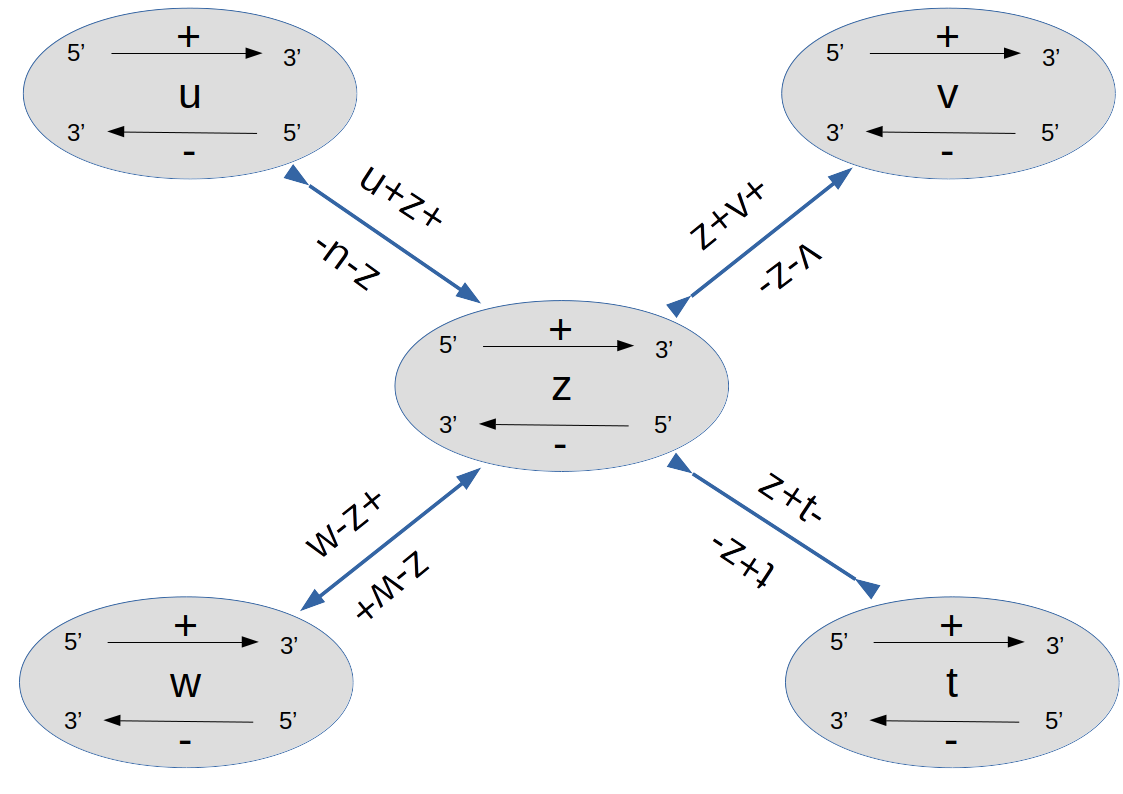
\includegraphics[width=.7\textwidth]{images/bgraph.png}
\caption[An example of bidirected graph model]
{An example of bidirected graph model. Each node contains a DNA sequence that can be spelled as template(+) or reverse complement(-). There are four possible types of a bidirected edge as shown as ones from node $z$. Each edge has two possible spelling depends on the starting node, resulting in two sequences of template and reversed complement. According to the rule of bidirected graph traversal, we have the following valid paths spelled as: $(u+,z+,v+)$, $(u+,z+,t-)$, $(w-,z+,v+)$, $(w-,z+,t-)$ and in the opposite direction respectively $(v-,z-,u-)$, $(t+,z-,u-)$, $(v-,z-,w+)$, $(t+,z-,w+)$.}
\label{f:bgraph}
\end{figure}

%bidirected graph
Assembly graph is normally implemented by using a directed graph data structure. 
In which, each component (vertex or edge, depends on particular implementation) storing a string has a corresponding counterpart for that string in reversed complement order \cite{Zerbino2008}.
To have a more compact representation of the graph, we employ the bidirected graph data structure instead.

%Formal definition of bidirected graph (convention on the GUI)
For a bidirected graph $G=\{V,E\}$, each edge has two directions associated with two nodes forming it. The direction here refers to a binary value that represent either incoming or outgoing state.
Unlike an edge in a directed graph, a bidirected edge can be traversed in both ways, similar to the property of an undirected edge except the content of each traversed vertex is not unique, but direction-wised. This means that if there exist a path from node A to B (or B is reachable from A) then the reversed path is legal as well (A is reachable from B), with a reverse-complemented spelling manner. 
Thus another equivalent interpretation for bidirected graph is an undirected graph of \emph{directed vertices}, which can be related directly to the purpose of modeling connections of DNA sequences as nodes in a graph structure, regarding they are double-stranded (sense and anti-sense). 
The edge-based modeling, in short, is more intuitive to work with; however in terms of comprehensive understandings and implementations, the directed-node ideology is additionally helpful.

\paragraph{Edge-based modeling} From this point of view, any edge $e \in E$ connecting an ordered pair of node $(u,v) \in V^2$ would fall into one out of four categories: $\blacktriangleright\blacktriangleright$, $\blacktriangleright\blacktriangleleft$, $\blacktriangleleft\blacktriangleright$ or $\blacktriangleleft\blacktriangleleft$. By modeling edge directions as such, the graph traversal is able to cover the double-stranded property of the DNA sequences (template/reverse complement) in vertices through edge-walking. 
The rule is that if we follow the arrow, its associated vertex is spelled as it is (+) and if we traverse against the arrow direction, the corresponding vertex is spelled as reverse complement sequence (-). As mentioned before, there are 2 ways of traversing through an edge, \EG from u to v and from v to u, as illustrated in Figure~\ref{f:bgraph}.
\paragraph{Vertex-based modeling} From this angle, it is convenient to firstly introduce the definition of directed node,  $\overrightarrow{v}=(v,d_v) \in \overrightarrow{V}$, as a tuple of vertex $v$ and its associated direction $d_v \in D=\{in,out\}$.
In this case, a bidirected edge is almost similar to an undirected edge connecting two (directed) vertices, \EG an unique edge that connect $\overrightarrow{u}$ and $\overrightarrow{v}$ can be equally written as $(\overrightarrow{u}, \overrightarrow{v})$ or $(\overrightarrow{v}, \overrightarrow{u})$. These two forward and reverse edges would refers to the same bidirected edge, except the content will be different depending on the order of spelled directed nodes.

The two definitions are equivalent and their applications are interchangeable and cohesive in our implementation. In summary, the meaning and spelling for a bidirected graph components is as follow:
\begin{itemize}
\item $u\blacktriangleright\blacktriangleright v$ equivalent to $(u-out, v-in)$: spelling $u+v+$ or $v-u-$
\item $u\blacktriangleright\blacktriangleleft v$ equivalent to $(u-out, v-out)$: spelling $u+v+$ or $v-u-$
\item $u\blacktriangleleft\blacktriangleright v$ equivalent to $(u-in, v-in)$: spelling $u-v+$ or $v-u+$
\item $u\blacktriangleleft\blacktriangleleft v$ equivalent to $(u-in, v-out)$: spelling $u-v-$ or $v+u+$
\end{itemize}

To create a valid path when traversing a bidirected graph, two adjacent edges must obey the direction rule similar to a conventional directed graph, that is a path which has an edge entering an intermediate node (not 2 ending nodes) must leave that node on the next edge. In addition, due to the allowance of traversing against the arrows in bidirected graph, it is possible to follow edges against their direction but the spelling will be reverse-complemented.

\section{Application of the assembly graph in \npscarfg{}}\label{sec:npscarfwag}
The first attempt of utilizing assembly graph is to integrate this pieces of information into the scaffolding algorithm for the gap-filling step thus increasing the accuracy of the final assembly. This is due to the fact that the edges from assembly graph come from Illumina data with much higher accuracy (99.9\%) compared to nanopore data ($\approx$90\%), which usually require high abundance to generate a consensus read with comparative quality. 

As shown in Figure~\ref{f:gapfilling}, for the first approach of gap filling, which is implemented in the very first version of \npscarf{}, segments from nanopore reads corresponding to a gap are first extracted based on the alignments to the flanking regions. A set of these pileup segments are then undergone a consensus calling step by multiple sequence aligner \EG{} \emph{kalign} \cite{LassmannFS2009} or \emph{poaV2} \cite{Lee2002multiple,Lee2003generating,Grasso2004combining}, and the result sequence can later be used to fill in the gap. 

\begin{figure}[!ht]
\centering
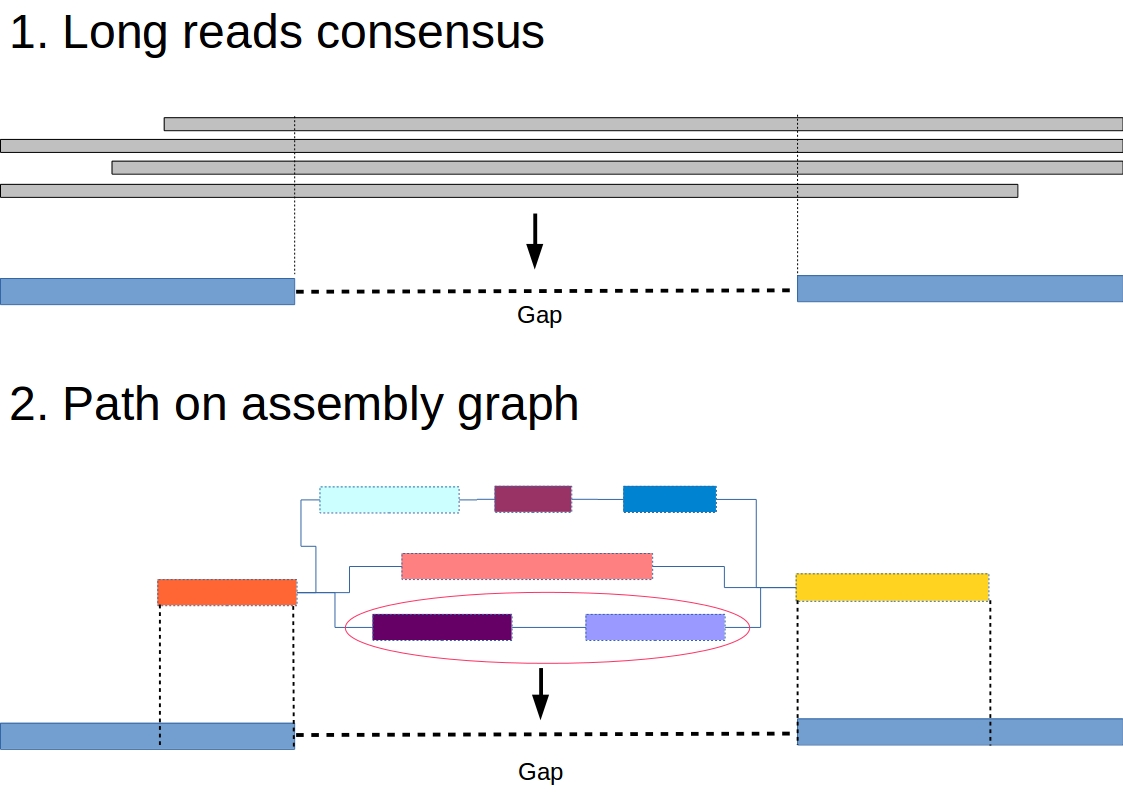
\includegraphics[width=.7\linewidth]{images/gapfilling.jpg}
\caption[Two approaches for gap filling in our methods.]
{Two approaches for gap filling: 1. using consensus sequences from long reads in \npscarf{}  and 2. using corresponding path in the assembly graph in \npscarfg{} .}
\label{f:gapfilling}
\end{figure}

Another \npscarf{} version, namely \npscarfg{}, utilizes assembly graph information for the gap filling step. In which, assembly graph from SPAdes is also learned together with contigs used as pre-assemblies in the workflow shown in Figure~\ref{f:workflow}. It is worth mentioning that each of these contigs is made of a path by traversing the assembly graph and normally short-read assemblers allow backtracking this piece of information, \EG{} via "\emph{contigs.paths}" file output from \spades{}. 

Mathematically, of this thesis' scope, a (bidirected) path $p\in P$ in (bidirected) graph $G\{V,E\}$ is defined as a walk through a series of alternative vertices and edges that are connected together, given that the bidirected transition rule holds true for every intermediate vertices. For example, from the edge-based modelling point of view, a path $p$ of size $k$ can be written as $p=\{v_0,e_1,v_1,e_2,v_2,\dots,v_{k-1},e_{k},v_k\}$ where $e_i$ is the bidirected edge connects $v_{i-1}$ and $v_{i+1}$ with every $1 \leq i < k$ and will determine the their directions in the walk. A path of size 0 contains only one vertex and no edge.
Importantly, the transition rule requires $dir(e_{i}, v_{i}) \neq dir(e_{i+1}, v_{i})$, $\forall 1 \leq i < k$ where $dir:(E,V)\rightarrow D$ is the function that returns direction (from vertex-based modelling) of a vertex on a given edge.

Using this decomposition, the corresponding components of the assembly graph (consecutive nodes) that make up the corresponding flanking tips of the gap are identified. Then by applying a searching algorithm, \EG{} Depth-First Search (DFS), on the graph, a set of candidate paths connecting two tipping nodes are determined. By selecting the path that maximize the likelihood of the long reads, the gap can be filled up by the sequence spelled out from it as shown in Algorithm \ref{algo:fillgap}. 

\begin{algorithm}[H]
\DontPrintSemicolon
\KwData{Assembly graph $G\{V,E\}$}
\KwIn{Bridge $B=(contig_1, contig_2)$ with gap}
\KwOut{Sequence to fill in the gap of $B$}
\Begin{
$p_1:=decompose(G,contig_1)$ \tcp*{decompose first contig into graph components}
$p_2:=decompose(G,contig_2)$ \tcp*{decompose second contig into graph components}
$\overrightarrow{v_1}:=p_1$.peek() \tcp*{get the last directed vertex of $p_1$}
$\overrightarrow{v_2}:=p_2$.getRoot() \tcp*{get the first directed vertex of $p_2$}
$p:=DFS(G,\overrightarrow{v_1},\overrightarrow{v_2})$ \tcp*{find a path connect these 2 tips}
\Return{$p$.spell()}
}
\caption{Pseudo-code for filling gap with assembly graph in \npscarf2{}.}
\label{algo:fillgap}
\end{algorithm}

Theoretically, this approach can increase the accuracy of gap-filling step, however, it offers limited capacity in reducing the mis-assemblies. The reason is that the ending components of a contig can be repetitive, make it impossible to confirm a genuine bridge with the existence of a path connect two tips as above. 
To deal with this issue, the assembly graph should be applied completely to the scaffolding algorithm by using the graph components as the building blocks, in replacement of the independent contigs as in \npscarf{} and \npscarfg{}. This idea lead to the development of \npgraph{} - a graph-based tool that can finish genomes in real-time.
%%%%%%%%%%%%%%%%%%%%%%%%%%%%%%%%%%%%%%%%%%%%%%%%%%%%%%%%%%%%%%%%
%%%%%%%%%%%%%%%%%%%%%%%%% npGraph %%%%%%%%%%%%%%%%%%%%%%%%%%%%%%
\section{Resolve assembly graph in real-time by long reads with \npgraph{}}
\subsection{Introduction}
Streaming assembly methods have been proven to be useful in saving time and resources compared to the traditional batch algorithms with examples included \EG $\mathtt{Faucet}$~\cite{Rozov2017faucet} and \npscarf{}~\cite{Cao2017scaffolding}. The first method allows the assembly graph to be constructed incrementally as long as reads are retrieved and processed. This practice is helpful dealing with huge short-read dataset because it can significantly reduce the local storage for the reads, as well as save time for a DBG construction while waiting for the data being retrieved.

\npscarf{}, on the other hand, works on the available short-read assembly to scaffold the contigs using nanopore sequencing which is well-known by the real-time property. The completion of genome assembly along with the sequencing run provides explicit benefits in term of resource control and turn-around time for analysis~\cite{Cao2017scaffolding}.  
However, due to the greedy approach of a streaming algorithm, as well as being an alignment-based-only scaffolding mechanism, running the tool with default settings suffers from mis-assemblies~\cite{Wick2017unicycler,Giordano2017}. In many case, the gap filling step has to rely on the low quality nanopore reads thus the accuracy of the final assembly is affected as well. 
To tackle the quality issue while maintaining its streaming execution, an assembly graph processing system is investigated as it would provide an additional high-quality source of linking information for the assembly operations. 

After the construction of an assembly graph, the next step is to traverse the graph, resolve the repeats and identify the longest possible un-branched paths that would represents contigs for the final assembly.
Hybrid assembler using nanopore data to resolve the graph has been implemented in $\mathtt{hybridSPAdes}$ \cite{AntipovKM2015} or \unicycler{} \cite{Wick2017unicycler}. 
In general, the available tools employ batch-mode algorithms on the whole long-read dataset to generate the final genome assembly. 
In which, the \spades{} hybrid assembly module, from its first step, exhaustively looks for the most likely paths (with minimum edit distance) on the graph for each of the long read given but only ones supported by at least two reads are attained. In the next step, these paths will be subjected to a decision-rule algorithm, namely $\mathtt{exSPAnder}$~\cite{Prjibelski2014}, for repeat resolution by step-by-step expansion, before output the final assembly.
On the other hand, \unicycler{}'s hybrid assembler will initially generate a consensus long read for each of the bridge from the batch data. 
The higher quality consensus reads are used to align with the assembly graph to find the best paths bridging pairs of anchored contigs.
While the later approach employs the completeness of the data  set from the very beginning for a consensus step, the former only iterates over the batch of possible paths and relies on a scoring system for the final decision of graph traversal. For that reason, the first direction is more suitable for a real-time pipeline.
    
However, the challenges to adapt this approach into a real-time mechanism are obvious and mainly come from the heavy path-finding task and the complication of self-improvement step which is critical to a streaming algorithm. 
A modified DFS algorithm and a voting system with accumulating scores calculation has been implemented to overcome these issues.
This results in \npgraph{}, an user-friendly tool with GUI that can traverse the assembly graph and scaffold its components in real-time as long as the nanopore sequencing process is running and continuously generating long reads.  


\subsection{Methods}
\subsubsection{Overview}
The input consists of Illumina assembly graph resulted from running assembler, e.g. \spades{}~\cite{BankevichNA2012}, $\mathtt{Velvet}$ \cite{Zerbino2008}, $\mathtt{AbySS}$ \cite{Simpson2009} on Illumina short reads, together with long reads from third generation sequencing technology (Oxford Nanopore Technology, Pacbio).
The long reads will be aligned with the contigs in the assembly graph to indicate longer paths that should be traversed. These local paths, given sufficient data, are expected to untangle the complicated graph and guide to the global Eulerian paths (or cycles if possible) that represent the entire genomic sequences. 

Basically the work flow of \npgraph{} can be divided into 3 main phases: abundance binning, graph resolving and assembly output. 
The first step is to bin the contigs into different groups of \emph{population} based on their coverage. 
Each population would include contigs of the similar abundance in the final assembly sequences, \EG{} chromosome , plasmids, or even particular species genome in a metagenomics community.
The binning phase would assist to differentiate between repetitive contigs and unique ones as well. By using this information, in combination with paths inducing from long reads, the assembly graph is then traversed and resolved in real-time. Finally, the graph is subjected to the last attempt of resolving and cleaning, as well as output the final results. The whole process can be managed by using either command-line interface or GUI.
\subsubsection{Pre-processing: identify repeat and unique contigs}
The purpose of this step is to investigate the sequencing properties of contigs, \IE{} length and \emph{k-mer} count, in combination with the graph topology, for an initial binning algorithm to determine multiplicity for each of them.
%\paragraph{Correct coverage bias due to GC content}
%The read coverage from Illumina data could be rectified by applying GC-content correction model \cite{BenjaminiS2012}.
%To be implemented.

\paragraph{Initial binning contigs into groups of abundances}
Each contig is represented as a node in the assembly graph and an edge connecting two nodes indicates their overlap (link) properties.
This step is to cluster the significant nodes (longer than $10$Kbp) into different sets, namely \emph{core} groups, based on their degree and coverage values.

DBSCAN clustering algorithm \cite{Ester96adensity-based} is applied for this task.
The idea is to consider a coverage value of a significant contig (which can be split into more than 10,000 \emph{k-mers}) to be a sampled mean of a Poisson distribution (of \emph{k-mers} count). 
The metric is a distance function based on Kullback-Leibner divergence \cite{Kullback1951information}, or relative entropy, of two Poisson distributions.

Assume there are 2 Poisson distribution $P_1$ and $P_2$ with density functions 
\begin{equation}
    p_1(x,\lambda_1)=\frac{e^{-\lambda_1}\lambda_1^x}{\Gamma(x+1)}
\end{equation}
and 
\begin{equation}
    p_2(x,\lambda_2)=\frac{e^{-\lambda_2}\lambda_2^x}{\Gamma(x+1)}
\end{equation}
The Kullback-Leibner divergence from $P_2$ to $P_1$ is defined as:
\begin{equation}
    D_{KL}(P_1||P_2)=\int_{-\infty}^{\infty} p_1(x)\log{\frac{p_1(x)}{p_2(x)}} dx
\end{equation}
or in other words,  it is the expectation of the logarithmic difference between the probabilities $P_1$ and $P_2$, where the expectation is taken with regard to $P_1$.

The log ratio of the density functions is
\begin{equation}
\log{\frac{p_1(x)}{p_2(x)}}=x\log{\frac{\lambda_1}{\lambda_2}}+\lambda_2-\lambda_1
\end{equation}
take expectation of this expression with regard to $P_1$ with mean $\lambda_1$ we have
\begin{equation}
D_{KL}(P_1||P_2)=\lambda_1\log{\frac{\lambda_1}{\lambda_2}}+\lambda_2-\lambda_1
\end{equation}

The metric we used is the distance defined as
\begin{equation}
D(P_1,P_2)=\frac{D_{KL}(P_1||P_2)+D_{KL}(P_2||P_1)}{2}=\frac{1}{2}(\lambda_1-\lambda_2)(\log{\lambda_1}-\log{\lambda_2})
\end{equation}

\paragraph{Coverage re-estimation}
Due to the possible divergence of sequencing coverage relative to the real abundance of sequences, especially the short ones, an optimization step is implemented to alleviate this issue. The coverage measure of nodes (which represent contigs) are spread throughout the graph via edges that connect them for comparison and calibration. 
The assignment of coverage to edges is also helpful to identify multiplicity in later step. 

The re-estimation is basically carried out by following two steps.
\begin{itemize}
\item[1.] From nodes coverage, estimate edges' value by quadratic unconstrained optimization of the least-square function:
\begin{equation}
\frac{1}{2}\sum_{i}{l_i((\sum{e^{+}_{i}}-c_i)^2+(\sum{e^{-}_{i}}-c_i)^2}
\end{equation}
where $l_i$ and $c_i$ is the length and coverage of a node $i$ in the graph;

$\sum{e^{+}_{i}}$ and $\sum{e^{-}_{i}}$ indicates sum of the values of incoming and outgoing edges from $i$ respectively. 
The above function and be rewritten as:
\begin{equation}
f(x)=\frac{1}{2}x^TQx + b^Tx + r
\end{equation}
and then being minimized by using Newton or gradient method.
\item[2.] Update nodes' coverage based on itself and its neighbor edges' measures.
\end{itemize}
The calibration is iterative until no further improvements are made or a threshold loop count is reached.
\paragraph{Multiplicity estimation}
Based on the coverage values of all the edges and the graph's topology, we induce the copy numbers of every significant nodes (long contigs) in the final paths.
For each node, this could be done by investigating its adjacent edges and answering the questions of how many times it should be visited, from which abundance groups.
Multiplicities of insignificant nodes (of sequences with length less than $1,000$ bp) can be estimated in the same way but usually with less confident due to more complicated connections and greater variances of coverage values. 
For that reason, they are only used as augmented information to calculate candidate paths' score in the next step.

\subsubsection{Untangling assembly graph by stream of nanopore data.}
\paragraph{Building bridges in real-time}
Bridge is the data structure designed for tracking the possible connections between two unique contigs (anchor nodes in the assembly graph). This approach was implemented in \npscarf{} gap-filling phase with assembly graph as in Figure \ref{f:gapfilling}.
% how bridge is connected, transformed multiplicity (real-time)
Here we take advantage of the graph topology and nodes' multiplicity information to employ a dynamic bridging mechanism.
This procedure considers the dynamic changing of multiplicity property for each node, meaning that a $n$-times repetitive node can become a unique node at certain time point when its $(n-1)$ occurrences are identified and assigned in appropriate unique paths. 

Other than \npscarf{}, a bridge in \npgraph{} has several completion levels. A bridge is only created with at least one unique contig as an end, if so it has level 1 of completion. If both ends are identified, the level is 2. The number is greater than that only if paths connecting two ends are found. A bridge is known as fully complete (level 4) if there is only one unique linking path left. Given a bridge with 2 ends, a path finding algorithm (described in next section) is invoked to find all candidate paths. Each of these paths is given a score of alignment-based likelihood which are updated immediately as long as there is an appropriate long read being generated by the sequencer. As more nanopore data arrives, the divergence between candidates' score becomes greater and only the best ones are voted for the next round.

Whenever a bridge becomes complete thanks to the voting system, the assembly graph is \emph{transformed} or \emph{reduced} by replacing its unique path by an composite edge and removing any unique edges (edges coming from unique nodes) along the path. The assembly graph would have at least one edge less than the original after the reduction. The nodes located on the reduced path, other than 2 ends, also have their multiplicities subtracted by one and the bridge is marked as finally resolved without any further modifications. 
\paragraph{Path finding algorithm}

\begin{algorithm}[!hpt]
\DontPrintSemicolon
\KwData{Assembly graph $G\{V,E\}$}
\KwIn{Bridge $B=(\overrightarrow{v_1}, \overrightarrow{v_2})$ with two ending unique bidirected nodes $\overrightarrow{v_1}, \overrightarrow{v_2}$}
\KwOut{Set of candidate paths $P$ connecting $B$}
\Begin{
$d$:=$B.length()$ \tcp*{length of the bridge or the distance between 2 ending nodes}
$M$:=$\mathtt{shortestTree}(\overrightarrow{v_2},d)$ \tcp*{build shortest tree from $\overrightarrow{v_2}$ with range $d$}
\If{$M.contain(\overrightarrow{v_1})$}{
    $S$:=new $Stack()$ \tcp*{stack of sets of edges to traverse}
    $edgesSet$:=$getEdges(\overrightarrow{v_1})$ \tcp*{get all bidirected edges going from $\overrightarrow{v_1}$}
    $S.push(edgesSet)$\;
    $p$:=new $Path(\overrightarrow{v_1})$ \tcp*{init a path that has $\overrightarrow{v_1}$ as root}
    \While{true}{
        $edgesSet$:=$S.peek()$\;
        \If{$edgesSet.isEmpty()$}{
            \If{$p.size() \leq 1$}{
                $\mathbf{break}$ \tcp*{stop the loop when there is no more edge to discover}
            }
        $S.pop()$\;
        $d$+=$p.peekNode.length()+p.popEdge().length()$\; 
        }
        \Else{
            $curEdge \coloneqq edgesSet.remove()$\;
            $\overrightarrow{v}$:=$curEdge.getOpposite(p.peekNode())$\;
            $S.push(getEdges(\overrightarrow{v}).includedIn(M))$\;
            $p.add(curEdge)$\;
            \If{reach $\overrightarrow{v_2}$ with reasonable $d$}{
                $P.add(p)$\;
            }
            $d$-=$\overrightarrow{v}.length()+curEdge.length()$\;
        }
    }
}


\Return{$P$}
}
\caption{Pseudo-code for finding paths connecting a bridge with 2 ends.}
\label{algo:findpath}
\end{algorithm}
% formal mathematical definition & DFS algorithm goes here...
In \npscarf{} with assembly graph, the path finding algorithm is the original DFS (depth first search) which becomes computationally expensive when the traversing depth increases. For \npgraph{}, we implement a modified stack-based version utilizing Dijkstra's shortest path finding algorithm~\cite{Dijkstra1959} to reduce the search space.

Algorithm~\ref{algo:findpath} demonstrates the path finding module in general.
In which, function 

$\mathtt{shortestTree}(\overrightarrow{vertex},distance) : (V,Z) \rightarrow V^n$ 

from line 3 of the algorithm's pseudo code builds a shortest tree rooted from $\overrightarrow{v}$, following its direction until a distance of approximately $d$ (with a tolerance regarding nanopore read error rate) is reached. This task is implemented based on Dijkstra algorithm.
This tree is used on line 4 and in function $includedIn()$ on line 19 to filter out any node or edge with ending nodes that do not belong to the tree.

Basically, the algorithm keeps track of a stack that contains sets of candidate edges to discover. During the traversal, a variable $d$ is updated as an estimation for the distance to the target. A hit is reported if the target node is reached with a reasonable distance \IE{} close to zero, within a given tolerance (line 21). 
A threshold for the traversing depth is set (150) to ignore too complicated and time-consuming path searching.

It is worth to mention that the $length()$ functions for node and edge are totally different. While the former returns the length of the sequence represented by the node, \IE{} contig from short-read assembly, the latter is usually negative because an edge models a link between two nodes, which is normally an overlap (except for composite edges). For example, in a \emph{k-mers} DBG-derived assembly graph, the value of an edge is $-k$. 

\subsubsection{Result extraction and output}
\npgraph{} reports assembly result in real-time by decomposing the assembly graph into a set of longest straight paths (LSP), each of the LSP will present a contig for the result.
A path $p=\{v_0,e_1,v_1,\ldots,v_{k-1},e_k,v_k\}$ of size $k$ is considered as straight if every edge along the path, $e_i, \forall i=1,\ldots,k$, must be the only option to traverse from either $v_{i-1}$ or $v_i$ following the transition rule.
To decompose the graph, we can just simply mask out all incoming/outgoing edges rooted from any node with in/out degree greater than 1 as demonstrated in Figure~\ref{figure:npgraph_decompose}. These edges are defined as branching edges which stop straight paths from further extending.

\begin{figure}[!hpt]
\centering
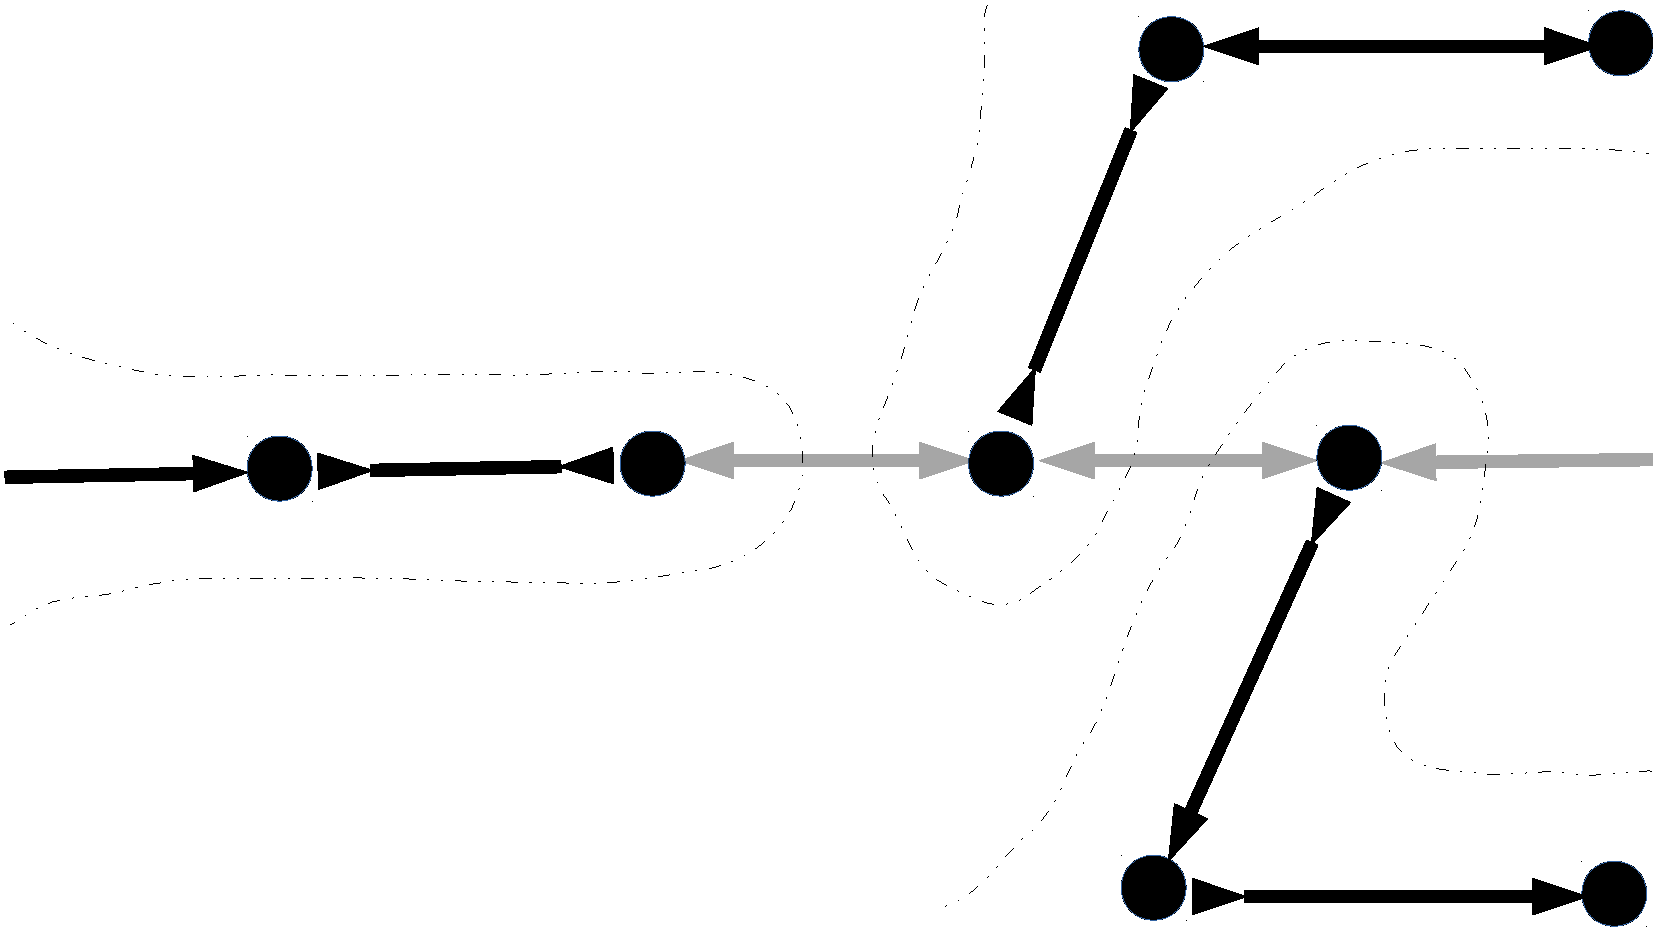
\includegraphics[width=.6\textwidth]{images/decompose.pdf}
\caption[Example of graph decomposition into longest straight paths]{Example of graph decomposition into longest straight paths. Branching edges are masked out (shaded) leaving only straight paths (bold colored) to report. There would be 3 contigs extracted by traversing along the straight paths here.}
\label{figure:npgraph_decompose}
\end{figure}
The decomposed graph is only used to report the contigs that can be extracted from an assembly graph at certain time point. For that reason, the branching edges are only masked but not removed from the original graph as they would be used for further bridging.

The final assembly output contains files in both FASTA and GFA v1 format (\url{https://github.com/GFA-spec/GFA-spec}). While the former only retains the actual genome sequences from the final decomposed graph, the latter output file can store almost every properties of the ultimate un-masked graph such as nodes, links and potential paths between them.
\subsubsection{User interface}
\begin{figure}[!hpt]
\centering
\parbox{\textwidth}{
    \parbox{.57\textwidth}{
        \subfloat{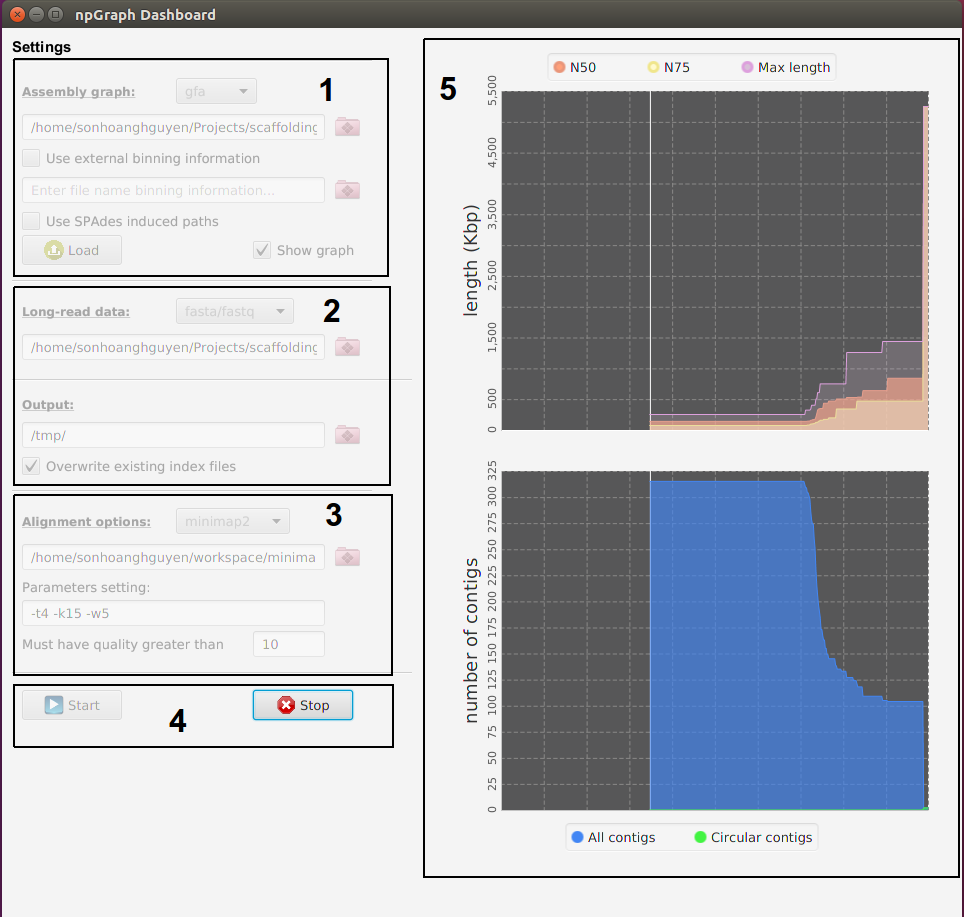
\includegraphics[width=\hsize]{images/dashboard.png}}
    }
    \hskip1em
    \parbox{.44\textwidth}{%
        \subfloat{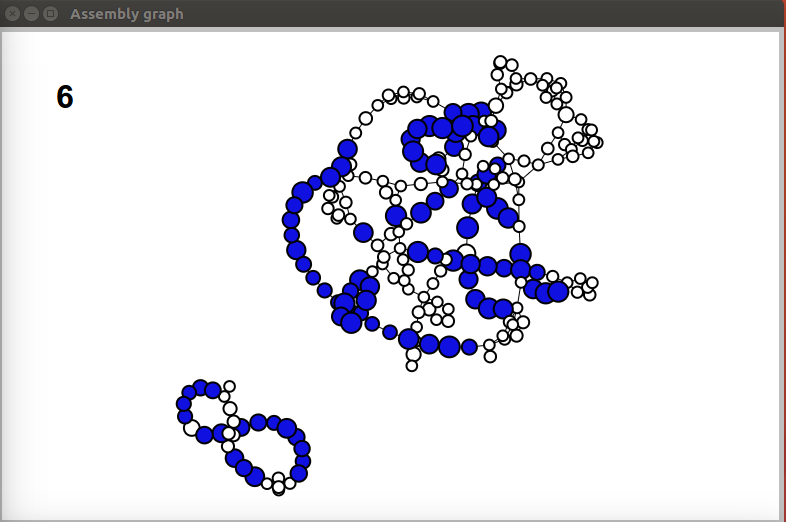
\includegraphics[width=\hsize]{images/graph-view.png}}
        \vskip1em
        \subfloat{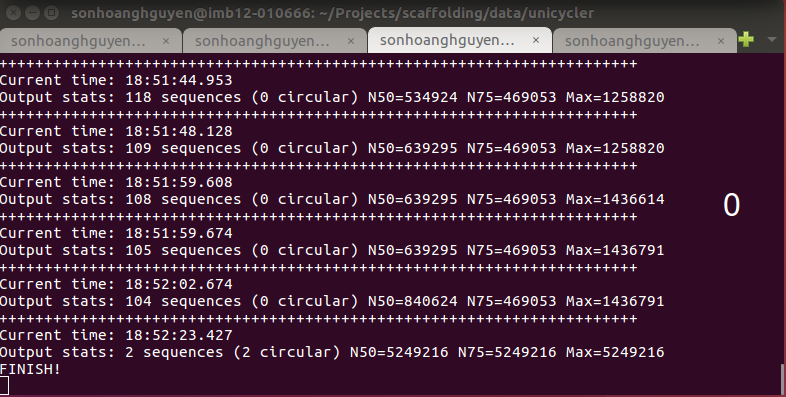
\includegraphics[width=\hsize]{images/console-view.png}}  
    }
}
\caption[\npgraph{} user interface]{\npgraph{} user interface including Console (\textbf{0}) and GUI components (\textbf{1}-\textbf{6}). The GUI consists of the Dashboard (\textbf{1}-\textbf{5}) and the Graph View (\textbf{6}). From the Dashboard there are 5 components as follow: \textbf{1} the assembly graph input field; \textbf{2} the long reads input field; \textbf{3} the aligner settings field; \textbf{4} control buttons (start/stop) to monitor the real-time scaffolding process; \textbf{5} the statistics plots for the assembly result.}
\label{figure:npgraph_gui}
\end{figure}

\npgraph{} can be invoked and fully function from the command-line interface. In addition, in order to aid the visualization of the assembly process, a GUI has been developed as well.

The GUI includes the dashboard for control the settings of the program and another pop-up window for a simple visualization of the assembly graph in real-time (Figure~\ref{figure:npgraph_gui}).
In this interface, the assembly graph loading stage is separated from the actual assembly process so that users can check for the graph quality first before carry out any further tasks. The box numbered \textbf{1} on Figure~\ref{figure:npgraph_gui} is designed for this task.
Only after an assembly graph is loaded successfully, users can move to box \textbf{2} to specify the nanopore input data.
Settings for an aligner (\bwa{} or \minimap{}) in box \textbf{3} is required if the input is the raw sequences in FASTA/FASTQ format. Another option is to run the alignment independently and provide SAM/BAM input for the next stage of bridging and assembly. This stage is controlled by buttons in box \textbf{4}: the START button ignites the process while the STOP button can prematurely terminate it and output the assembly result till that moment. The plots from the right panel (\textbf{5}) depicts real-time statistics of the assembly contigs inferred from the graph.
From the second window (\textbf{6}), the colored vertices imply unique contigs while the white ones involve either unspecified or repetitive elements. The number of different colors (other than white) indicates the amount of abundant groups being detected as population bins (\EG{} chromosome versus different plasmids, or different bins in metagenomics).

A proper combination of command line and GUI can provide an useful streaming pipeline that copes well with MinION output data. The practice is similar to the previous developed pipelines~\cite{CaoGC2016,Cao2017scaffolding,Nguyen2017barcode} that allow the analysis to take place abreast to a nanopore sequencing run.
\subsection{Results}
\subsubsection{Hybrid assembly for synthetic datasets}
To evaluate the performance of the method, \npgraph{} was benchmarked against \spades{} with its hybrid assembly module~\cite{AntipovKM2015}, \npscarf{} with/without assembly graph integrated, and Unicycler version 0.4.6 on the latter's testing data~ \cite{Wick2017unicycler} . This dataset were simulations of Illumina and MinION raw data, generated \emph{in silico} based on random and available microbial references. 
Specifically, the synthetic Illumina data was generated by using a wrapper script of ART~\cite{HuangLMM2012} that allows uniform coverage for circular genome sequencing with justifiable depths.
PBSIM~\cite{OnoAH2012}, on the other hand, was used to simulate the long reads.

There were three settings for each of the synthetic raw data (\emph{good, medium, bad}) corresponding to the quality, yield and length of reads being generated. 
In the SGS simulation, the \emph{bad} data consist of 100bp paired-end reads with low and uneven coverage (40X) leading to many dead ends in the assembly graph due to missing regions in the genome. 
The read length was 125bp in the \emph{medium} setting with better depth distributions that could cover the genome better. 
Finally, the \emph{good} option provided best datasets with 150bp of read length and 100X coverage.
While the quality of SGS reads would determine the assembly graph nature, the nanopore data plays critical role in graph resolving.
The three settings leveled up the depth (8X, 16X, 32X) and at the same time, average length ($5$Kbp, $10$Kbp, $20$Kbp) and maximum identities (90\% ,95\% ,98\%) respectively.
We only considered the \emph{good} configurations of both platforms for the sequence data being tested.
Also, since the other comparative tools do not support streaming assembly, there were only batch-mode runs being carried out and the reciprocal results were examined by QUAST 5.0.2~\cite{Mikheenko2018quast5}. 

\LTcapwidth=\linewidth
\footnotesize
\begin{longtable}{llcrrrrr@{\hspace{2pt}}c@{\hspace{2pt}}r}
\caption[Comparison of assemblies using \npgraph{} and other comparative methods on 5 synthetic datasets]{Comparison of assemblies produced in batch-mode using \npgraph{} and the comparative methods on 5 synthetic datasets taken from \url{https://cloudstor.aarnet.edu.au/plus/index.php/s/dzRCaxLjpGpfKYW}} \label{table:npgraph_compare} \\

 \toprule
    &       & \cthead{1}{Assembly} &     & 
    \cthead{1}{N50}  & \cthead{1}{Mis-} &  \cthead{1}{Error}  &
    \cthead{3}{Run times} \\
    & \cthead{1}{Method} & \cthead{1}{size (Mb)} & \cthead{1}{\#Contigs} &
    \cthead{1}{(Kp)} & \cthead{1}{assemblies} & \cthead{1}{(per 100 Kb)} &  
    \cthead{3}{(CPU hrs)} \\
\toprule    
\endfirsthead

\multicolumn{10}{c}%
{{\tablename\ \thetable{} -- continued from previous page}} \\
 \toprule
    &       & \cthead{1}{Assembly} &     & 
    \cthead{1}{N50}  & \cthead{1}{Mis-} &  \cthead{1}{Error}  &
    \cthead{3}{Run times} \\
    & \cthead{1}{Method} & \cthead{1}{size (Mb)} & \cthead{1}{\#Contigs} &
    \cthead{1}{(Kp)} & \cthead{1}{assemblies} & \cthead{1}{(per 100 Kb)} &  
    \cthead{3}{(CPU hrs)} \\
\toprule    
\endhead

\hline \multicolumn{10}{|r|}{{Continued on next page}} \\ \hline
\endfoot

\hline \hline
\endlastfoot

\rowcolor{Gray} \multicolumn{10}{l}
{ random sequence with repeats} \\*  
 & SPAdes  & 3.928 & 226  & 40.5  &  0 &  0.00 &  0.95 &  &  \\*
 & SPAdes-Hybrid  & 4.109 & 3  & 4,000.0  & 0  & 0.85  & 1.196  &  &  \\*
 & Unicycler  & 4.110 & 3  & 4,000.0  &  0 &  0.47 & 6.783  &  &  \\*
 & npScarf  & 4.251 &  9 & 3,952.2  &  27 &  8.74 &  0.95 & + & 0.39 \\*
 & npScarf\_wag & 4.554 & 9  &  3,999.6 &  37 &  6.16 &  0.95 & + &  0.45\\*
 & npGraph (bwa)  & 4.110 & 3  & 4,000.0  & 0  &  0.47 &  0.95 & + &  0.33\\*
 & ngGraph (minimap2)  & 4.110 & 3  & 4,000.0  & 0  & 0.47  &  0.95 & + &  0.02\\
\rowcolor{Gray} \multicolumn{10}{l}
{\emph{Mycobacterium tuberculosis} H37Rv} \\*  
 & SPAdes  & 4.371 & 114  &  125.5 &  1 & 1.51  &  1.55 &  &  \\*
 & SPAdes-Hybrid  & 4.411 & 1  & 4,411.2  & 0  & 1.73  & 1.68  &  &  \\*
 & Unicycler  & 4.412 &  1 &  4,411.5 & 0  &  2.56 &  6.36 &  &  \\*
 & npScarf  & 4.446 & 4  & 4,389.9  & 12  &  11.41 & 1.55  & + & 0.78 \\*
 & npScarf\_wag  & 4.408 & 1  & 4,407.6  &  2 &  7.01 & 1.55  & + & 0.79 \\*
 & npGraph (bwa)  & 4.411 &  1 & 4,411.6  &  0 & 7.28  &  1.55 & + & 0.63 \\*
 & ngGraph (minimap2)  & 4.411 & 1 & 4,411.4  &  0 &  7.01 & 1.55  & + &  0.02\\
\rowcolor{Gray} \multicolumn{10}{l}
{\ec{} O25b H4-ST131} \\*  
 & SPAdes  & 5.173 &  159 & 191.0  &  1 &  1.69 & 1.26  &  &  \\*
 & SPAdes-Hybrid  & 5.249 &  7 &  5,109.6 & 0  & 2.65  & 1.40  &  &  \\*
 & Unicycler  & 5.249 &  3 & 5,109.8  &  0 &  4.29 &  4.70 &  &  \\*
 & npScarf  & 5.354 & 7  & 5,087.5  &  14 & 29.12  &  1.26 & + &  0.78\\*
 & npScarf\_wag  & 5.413 &  7 & 5,108.1  & 6  &  30.29 & 1.26  & + & 0.78 \\*
 & npGraph (bwa)  & 5.252 & 3  &  5,112.3 &  0 & 16.37  & 1.26  & + &  0.66\\*
 & ngGraph (minimap2)  & 5.250 & 3  & 5,111.1  & 0  & 14.61  &  1.26 & + & 0.03 \\
\rowcolor{Gray} \multicolumn{10}{l}
{\emph{Streptococcus suis} BM407} \\*  
 & SPAdes  & 2.119 &  81 &  131.0 & 0  & 3.84  & 0.59  &  &  \\*
 & SPAdes-Hybrid  & 2.147 & 48  &  1,438.0 &  0 &  0.98 & 0.65  &  &  \\*
 & Unicycler  & 2.171 &  2 &  2,146.2 & 0  &  2.99 &  2.58  &  &  \\*
 & npScarf  & 2.220 &  4 &  2,120.0  & 9  & 97.20  & 0.59 & + & 0.31 \\*
 & npScarf\_wag  & 2.245 & 4  &  2,128.3  & 3  &  89.64 & 0.59 & + &  0.31\\*
 & npGraph (bwa)  & 2.167 & 6  & 2,146.7  &  0 &  26.77 & 0.59  & + &  0.21\\*
 & ngGraph (minimap2)  & 2.167 & 6  &  2,146.2 &  0 & 22.53  &  0.59 & + & 0.01 \\
\rowcolor{Gray} \multicolumn{10}{l}
{\emph{Acinetobacter} AB30} \\*  
 & SPAdes  & 4.134 & 265  & 42.5  &  0 &  3.23 & 0.95  &  &  \\*
 & SPAdes-Hybrid  & 4.287 & 49  &  3,308.0 &  0 & 5.04  & 1.84  &  &  \\*
 & Unicycler  & 4.333 & 1  &  4,333.0 &  1 & 6.95  &  5.27 &  &  \\*
 & npScarf  & 4.595 & 11  & 4,299.7  & 1  & 120.99  & 0.95  & + & 0.45 \\*
 & npScarf\_wag  & - & -  &  - & -  &  - &  - &  &  \\*
 & npGraph (bwa)  & 4.317 & 6  &  2,766.9 & 1  &  39.82 &  0.95 & + & 0.41 \\*
 & ngGraph (minimap2)  & 4.337 & 1  &  4,336.8 & 0  & 24.71  & 0.95  & + & 0.03 \\
\end{longtable}

\normalsize

Table~\ref{table:npgraph_compare} shows evaluation results for 5 synthetic datasets, the output of the full run can be found in Table~\ref{supp_tab:synthetic_benchmark}.
In the first column of applied methods, beside \unicycler{} and $\mathtt{hybridSPAdes}$, \npscarf{} is included as the original scaffolder (described in Chapter~\ref{ch:npscarf}) and \npscarfg{} is the modified version with assembly graph integrated (this Chapter, Section~\ref{sec:npscarfwag}).
On the other hand, \npgraph{} can use 2 different aligners, \bwa{} and \minimap{}, for its bridging phase thus both practices were included in this comparison.

In general, the graph integrated version of \npscarf{} improved the assembly results in terms of mis-assemblies and error reduction while virtually consuming similar resources compared to the original version.
The only exception where the number of mis-assemblies being increased was the simulation of a random sequence with many repeats. There were 10 more mistakes detected using the later version \npscarfg{}. However, with additional investigations, we found that the number of mis-assemblies on the true positive circular sequences (3 from the reference) has been significant reduced by applying assembly graph for \npscarf{}. The errors mostly came from redundant sequences output from the software due to the failure in estimation of contig multiplicity.
Even though using assembly graph for gap fillings, there were no changes in the way to determine if a contig is unique or not from \npscarfg{}. 
It still relied on the length and coverage statistics, \IE{} \emph{Astats}~\cite{MyersSD2000} to find anchors that were critical for the backbone construction of the assembly.
Redundant path findings for false positive replicons consequently returned additional wrong translocations in the final contigs which were reported by QUAST. 
Other than that, the method had successfully produced better assemblies than the original. Regarding \emph{Mycobacterium tuberculosis} H37Rv, the number of mis-assembled breakpoints had been trimmed down from 12 to 2, while the number of final contigs had reduced from 4 to only one as in the reference. Results in cases of \ec{} O25b H4ST131 and \emph{Streptococcus suis} BM407 also showed enhancements in terms of those categories as well as N50 statistics. 
There was improvements considering the nucleotide errors (mismatches and indels) as well from aforementioned datasets, except for the \ec{} when slightly more mismatches had been detected. However, these errors can be corrected by running polishing tools with the raw Illumina data afterward. 

For \emph{Acinetobacter} AB30 synthetic data, it was an deficiency for \npscarfg{} in traversing the graph to find candidate paths for a bridge of long distance due to particular large search space.
The exhaustive, naive DFS implementation for this version of \npscarf{} required a lot of memory to traverse a complex assembly graph that usually exceed a normal desktop's capacity.
This issue has been fixed in \npgraph{} when Algorithm~\ref{algo:findpath} was used on the definitive graph. This resulted in completed runs of the assembly process for all datasets with the similar number of mis-assemblies compared to the best figures in this category.
As shown in Table~\ref{table:npgraph_compare} and \ref{supp_tab:synthetic_benchmark}, the assembly graph based methods offered significant improvements when compared to \npscarf{}. Not only because of the clear drops with respect to mis-assemblies and errors, but it was also reflected by the number of final contigs and their N50 as well.

To align the long reads to the assembly graph components, either \bwa{}~\cite{Li2013} or \minimap{}~\cite{Li2016} was invoked in \npgraph{}. 
The former option was inherited from \npscarf{} pipeline with the intact parameters
%$-k11 -W20 -r10 -A1 -B1 -O1 -E1 -L0 -a -Y$
while the latter was used with the recommended settings (-$\mathtt{k}$15 -$\mathtt{w}$5) for the best sensitivity working on MinION data.
Even though, \bwa{} normally reported more hits than \minimap{} but at the same time, was responsible for more false positive alignments.
For instance, regarding the last dataset from Table~\ref{table:npgraph_compare}, the assembly of \npgraph{} using \bwa{} was suffered from the ambiguous alignments thus more fragmented than the other counterparts. 
On the other hand, referring to more complicated graphs from \emph{Acinetobacter} A1 and the yeast \emph{Saccharomyces cerevisiae} S288c from Table~\ref{supp_tab:synthetic_benchmark}, the number of mis-assemblies from using \minimap{} were increased due to the lacks of appropriate alignments to support accurate bridging process.
However, under almost circumstances, using either aligners would result in final assemblies with similar qualities.
Furthermore, in terms of running time and resources required, \minimap{} proved to be the best option. 
The total CPU hours had been trimmed down drastically with the new aligner, making \npgraph{} the fastest hybrid assembler available.
This feature is certainly more favoured to a real-time assembly as well.
As the consequence, as long as \minimap{} is expected to replace \bwa{} for long-read sequencing data alignment, it would likewise become the main aligner for \npgraph{} pipeline in the future.

It is noteworthy to discuss in more details the errors addressed in the above assembly methods.
This figure measured the total mismatches and indels per 100kpb from the assembly sequences when mapping to the reference.
As expected from hybrid assemblies where Illumina sequencing data were used as the main building blocks, the figures were hardly bigger than 100 (equivalent to 0.1\% error rate) for almost every case.
In addition, the indels errors, which mainly caused by TGS data, were found relatively low in the final contigs (Table~\ref{supp_tab:synthetic_benchmark}).
The majority of the differences accounted for the mismatched nucleotides caused by the alternative paths connecting the unique anchors from the backbone of the assembly.
This phenomenon may root from homologous repeats or sequencing errors of the genome.
From all the hybrid assemblers, $\mathtt{hybridSPAdes}$ reported results with highest fidelity. This meant that the performance its decision-rule algorithm $\mathtt{exSPAnder}$~\cite{Prjibelski2014} was the most accurate amongst all path finding methods. As the trade-off, there were fewer connections satisfying its quality threshold, resulting in the fragmented assemblies in cases of \emph{Streptococcus suis} or \emph{Acinetobacter} samples (Table~\ref{table:npgraph_compare} and \ref{supp_tab:synthetic_benchmark}).
\unicycler{}, which employs an algorithm based on semi-global (or glocal) alignments~\cite{Brudno2003glocal} with the consensus long reads, returned the second best reliable and at the same time, closest-to-complete results overall.
\npscarf{}, on the other hand, exploited the long reads for the gap filling thus inherited the high error rates from them.
By integrating the assembly graph for the task, the errors were reduced in general (random sequences, \emph{M.~tuberculosis}, \emph{S.suis} from Table~\ref{table:npgraph_compare}) but not completely since the mis-placed contigs were still not resolved in other circumstances.
\npgraph{} significantly reduced the errors compared to \npscarf{}, however the figures were still higher than the those of the best counterparts.
This implied a more robust decision making system is needed in \npgraph{}'s real-time path finding module for even better output's accuracy.

\subsubsection{Hybrid assembly for real datasets}
Several sequencing datasets of actual bacterial samples~\cite{George2017M14} were used in this scenario.
The data included both Illumina paired-end and MinION sequencing based-call data for each sample.
Unlike previous settings, rather than the default output, the optimal \spades{} assembly graph detected by \unicycler{} were used for \npgraph{} algorithm as well.
This step had been proved to be useful in selecting the best graph available, amongst \spades{} runs with ranging $k$-mer values, that have dead-ends and number of contigs minimized~\cite{Wick2017unicycler}. Likewise, as mentioned before, the quality of the initial assembly graph would considerably influence the final results of \npgraph{}. 

Due to the lack of available reference genomes, fewer statistics were reported by QUAST for the comparison of the results. 
Instead, we investigated the number of circular sequences and $\mathtt{PlasmidFinder}$ 1.3~\cite{Carattoli2014} mappings to obtain an evaluation on the accuracy and completeness of the assemblies.
Table~\ref{tab:npgraph_real} shows the benchmark results of \npgraph{} (using \minimap{}) against \unicycler{} on three datasets of bacterial species \emph{Citrobacter~freundii}, \emph{Enterobacter~cloacae} and \emph{Klebsiella~oxytoca}. 

\begin{table}[!hpt]
\centering
\caption[Assembly of real datasets using \unicycler{} and \npgraph{} with the optimized SPAdes output]{Assembly of real datasets using \unicycler{} and \npgraph{} with the optimized \spades{} output. Circular contigs are highlighted in \textbf{bold}, fragmented assemblies are presented as X$\vert$Y where X is the total length and Y is the number of supposed contigs making up X.}
\label{tab:npgraph_real}
\begin{tabular}{p{4cm}rrl}
\hline
\toprule
 & \textbf{\unicycler{}} & \textbf{\npgraph{}} & \textbf{Replicons (based on $\mathtt{PlasmidFinder}$ 1.3)} \\ 
\hline 
\rowcolor{Gray}
 \cellcolor{white} \emph{Citrobacter freundii} & \textbf{5,029,534} & \textbf{5,029,486} & Chromosome \\
CAV1374 & \textbf{109688} & \textbf{109688} & IncFIB(pHCM2)\_1\_pHCM2\_AL513384 \\
\rowcolor{Gray}
 \cellcolor{white}  & \textbf{100,873} & \textbf{100,873} & IncFIB(pB171)\_1\_pB171\_AB024946 \\
 & \textbf{85,575} & \textbf{85,575} & IncL/M(pMU407)\_1\_pMU407\_U27345 \\
\rowcolor{Gray}
 \cellcolor{white}  & \textbf{43,621} & \textbf{43,621} & repA\_1\_pKPC-2\_CP013325 \\
 & \textbf{3,223} & \textbf{3,223} & - \\
\rowcolor{Gray}
 \cellcolor{white}  & \textbf{1,916} & \textbf{1,916} & ColRNAI\_1\_\_DQ298019 \\
 & 14,464$\vert$3 & 14,456$\vert$2 & - \\ \hline
\rowcolor{Gray}
 \cellcolor{white} \emph{Enterobacter cloacae} & 4,806,666$\vert$2 & 4,858,438$\vert$2 & Chromosome \\
CAV1411 & \textbf{90,451} & 90,693$\vert$2 & IncR\_1\_\_DQ449578 \\
\rowcolor{Gray}
 \cellcolor{white} & \textbf{33,610} & \textbf{33,610} & repA\_1\_pKPC-2\_CP013325 \\
 & 13,129$\vert$2 & 14,542$\vert$4 & - \\ \hline
\rowcolor{Gray}
 \cellcolor{white} \emph{Klebsiella oxytoca}  & 6,153,947$\vert$5 & \textbf{6,155,762} & Chromosome \\
CAV1015 & \textbf{113,105} & \textbf{113,105} & \begin{tabular}[c]{@{}l@{}}IncFII(SARC14)\_1\_SARC14\_JQ418540;\\ IncFII(S)\_1\_\_CP000858\end{tabular} \\
\rowcolor{Gray}
 \cellcolor{white} & \textbf{111,395} & \textbf{111,395} & - \\
 & \textbf{108,418} & 109,209$\vert$13 & IncFIB(K)\_1\_Kpn3\_JN233704 \\
\rowcolor{Gray}
 \cellcolor{white} & \textbf{76,183} & \textbf{76,186} & IncL/M(pMU407)\_1\_pMU407\_U27345 \\
 & \textbf{11,638} & 11,892$\vert$2 & - \\ \hline
\end{tabular}
\end{table}

From the first dataset, there was high similarity between final contigs generated by two assemblers.
They shared the same number of circular ultimate sequences, including the chromosomal and other six replicons contigs. 
The only divergence lied on the biggest sequence ($\simeq 5.029$Mbp) when the \unicycler{}'s chromosome was 48 nucleotides longer than that of \npgraph{}.
Five out of six identical replicons were confirmed as plasmids based on the occurrences of appropriate Origin of replication sequences (PlasmidFinder database).
In detail, two megaplasmids (longer than $100$Kpb) were classified as IncFIB while the other two mid-size replicons, $85.6$Kbp and $43.6$Kpb, were incL and repA respectively, leaving the shortest one with $2Kbp$ of length as ColRNAI plasmid.
The remaining circular sequence without any hits to the database was $3.2$Kbp long suggesting that it could be phage or newly replicon's DNA.
Lastly, there were still $14.5$Kbp unfinished sequences resulted in 3 linear contigs from \unicycler{} and 2 for \npgraph{} respectively.

The assembly task for \emph{Enterobacter~cloacae} was more challenging as the chromosomal DNA sequence was not been fully resolved using either method. 
The chromosome size was estimated to be approximately $4.8$Mbp but had been broken into two smaller pieces. 
\npgraph{} returned longer stretches of length $3.324$Mbp and $1.534$Mbp while the figures were $2.829$Mbp and $1.978$Mbp from \unicycler{}'s output.
However, the number of circular sequences detected by \unicycler{} was one more than the other ($2$ versus $1$). They were corresponding to 2 plasmids, namely IncR and repA.
While the latter were recognized by both methods, the longer plasmid sequence was fragmented running \npgraph{}.
Similar to the previous dataset, there were around $14$Kpb of data were unable to be finished by the assemblers.

Finally, assembly for \emph{Klebsiella oxytoca} saw fragmented chromosome using \unicycler{} but it was a fully complete contig for \npgraph{} with $6.156$Mbp of size.
The two assemblers shared 3 common circular sequences where two of them were confirmed plasmids. 
The first identical sequences represented a megaplasmid ($\simeq 113$Kbp) with two variations of IncFII's origin of replication DNA being identified. 
The other agreed plasmid were IncL/M with $76$Kbp of length.
Particularly, there was one circular contig with length greater than $100$Kbp but returned no hits to the plasmid database, suggesting the importance of \emph{de novo} replicon assembly in combination with further interrogations.
\unicycler{} detected another megaplasmid of size $108.4$Kbp which was fractured by \npgraph{}. 
The dissolution was also observed in \npgraph{} for the final contig of length $11.6$Kbp where it failed to combine two smaller sequences into one.

In addition to what presented in Table~\ref{tab:npgraph_real}, dot plots for the pair-wise alignments between the assembly contigs were generated and can be found in Appendix Figure~\ref{supp_fig:npgraph_dotplot}. Interestingly, beside all other agreements, there was a structural difference using two methods for \emph{E.~cloacae} CAV1411 genome assembly. This was caused by the inconsistency of a fragment's direction on the final output contigs. However, when compare to a reference genome of the same bacteria strain (GenBank ID: CP011581.1~\cite{Potter2016rapid}), contigs generated by \npgraph{} demonstrated a consistent alignment which was not the case for \unicycler{} results (Appendix Figure~\ref{supp_fig:npgraph_ref}). Even though this might reflect a novel variation between bacterial samples of the same strain, it was more likely a mis-assembly by using \unicycler{}.

Overall, by testing with synthetic and real data, \npgraph{} proved to be able to generate assemblies of comparative quality compared to other powerful batch-mode hybrid assemblers, such as $\mathtt{hybridSPAdes}$ or \unicycler{}.
Furthermore, similar to \npscarf{}, it has the advantage in term of supporting real-time assembly. The next section will address this utility and the interactive GUI bundled in \npgraph{}. 

\subsubsection{Real-time mode hybrid assembly}

\begin{figure}[!hpt]
\centering
\subfloat[\emph{Citrobacter~freundii} CAV1374]{
	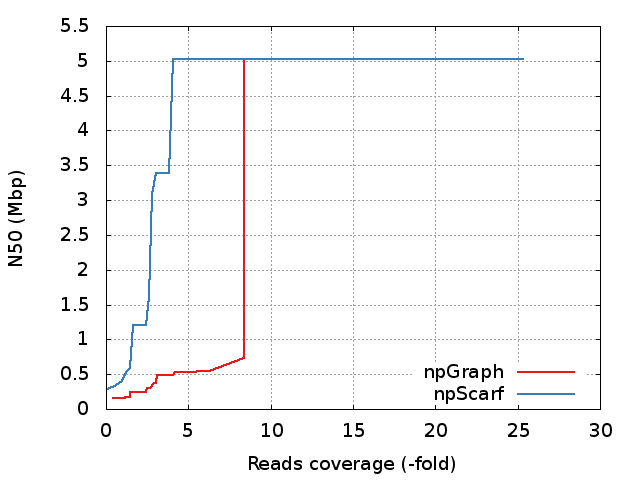
\includegraphics[width=.45\textwidth]{images/rt_cf1374.png}
}
\hfill
\subfloat[\emph{Escherichia~coli} K12 MG1655]{
	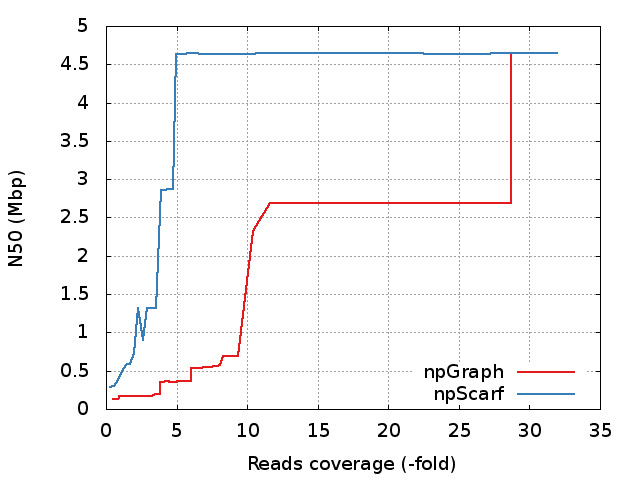
\includegraphics[width=.45\textwidth]{images/rt_eck12.png}
}
\\
\subfloat[\emph{Klebsiella} 30660 NJST258]{
	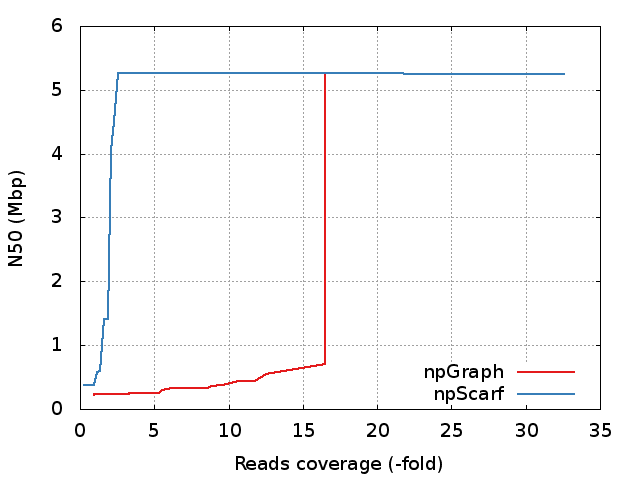
\includegraphics[width=.45\textwidth]{images/rt_kp30660.png}
}
\hfill
\subfloat[\emph{Klebsiella} NTUH K2044]{
	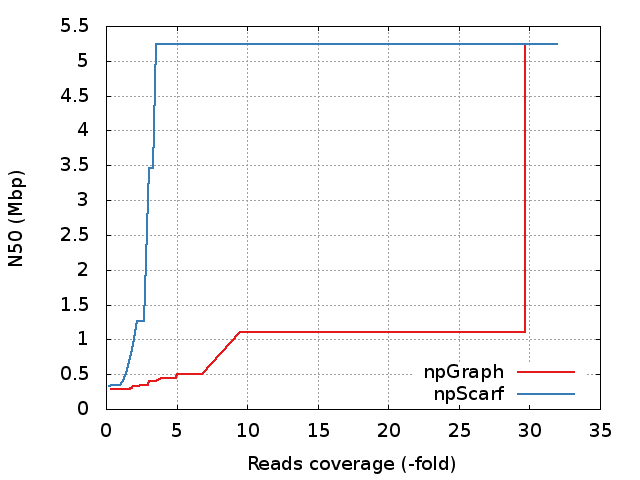
\includegraphics[width=.45\textwidth]{images/rt_kpntuh.png}
}
\caption[Real-time scaffolding by \npscarf{} versus \npgraph{}]{N50 statistics of real-time scaffolding by \npscarf{} versus \npgraph{}.}
\label{F:npgraph_rt}
\end{figure}

Figure~\ref{F:npgraph_rt} demonstrates the real-time mode performance of \npscarf{} and \npgraph{} via N50 statistics during the assembly of 4 example datasets.
This experiment would discover the rate of completing genome assemblies of the new method, set aside the accuracy aspect which had already been discussed previously.
\npscarf{}\_wg basically scaffolds the pre-assembly contigs in the same manner with the original version thus was not discussed here.

As can be observed from all the plots, \npgraph{} and \npscarf{} both converged to the same ultimate completeness but with different paces and patterns.
Apparently it took more data for \npgraph{} to finish the same genome than the other.
The reason stems from the fact that the new algorithm implemented a more `conservative' approach of bridge construction with at least 3 supporting long-reads for each to prevent any potential mis-bridging. 
Unlike \npscarf{} when the connections could be undone and rectified later if needed, a bridge in \npgraph{} will remain unchanged once created.
The plot for \ec{} data clarifies this behaviour when a fluctuation can be observed in \npscarf{} assembly at $\simeq 3$-folds data coverage.
On the other hand, the N50 length of \npgraph{} is always a monotonic increasing function. 
The sharp `jumping' patterns suggested that the linking information from long-read data had been stored and exploited at certain time point decided by the algorithm.
Once a unique path has been determined, the bridge can be formed to connect the fragments together into longer sequences.


\begin{figure}[!hpt]
\centering
\subfloat[Initial graph]{
	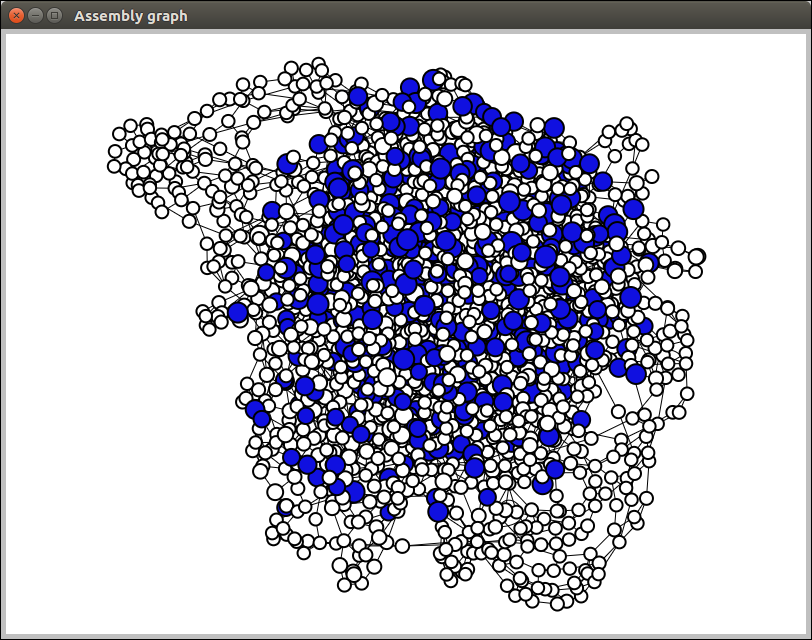
\includegraphics[width=.45\textwidth]{images/npgraph_shigella_0.png}
}
\hfill
\subfloat[Resolved graph]{
	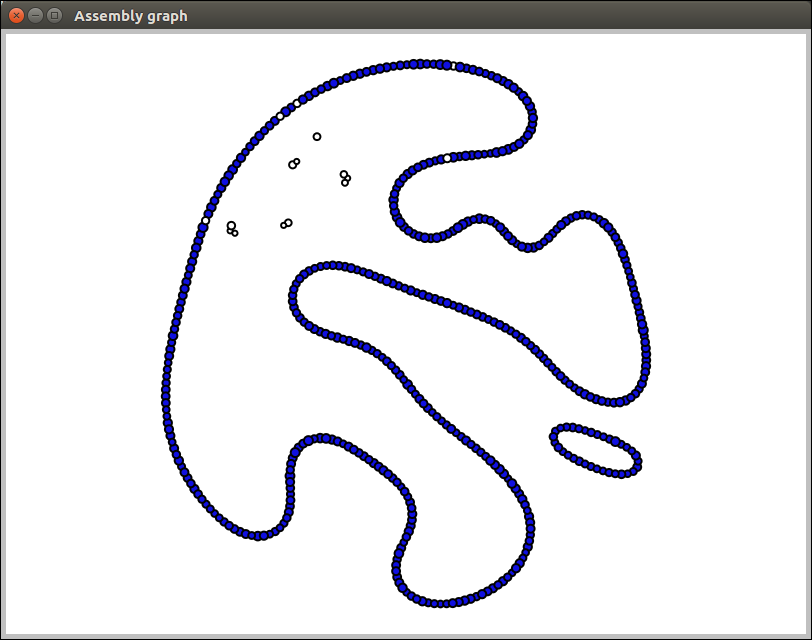
\includegraphics[width=.45\textwidth]{images/npgraph_shigella_2.png}
}
\caption[Assembly graph resolving on \npgraph{} Graph View]{Assembly graph of \emph{Shigella~dysenteriae} Sd197 synthetic data being resolved by \npgraph{} and displayed on the GUI Graph View. The \spades{} assembly graph contains 2186 nodes and 3061 edges, after the assembly shows 2 circular paths representing the chromosome and one plasmid.}
\label{F:npgraph_graphview}
\end{figure}

Figure~\ref{F:npgraph_graphview} shows an example of the real-time graph resolving process being displayed on GUI.
The result graph, after cleaning, would only report the significant connected components that represents the final contigs.
Smaller fragments, even unfinished but with high remaining coverage, are also presented as potential candidates for further downstream analysis.
Further annotation utility can be implemented in the future better monitoring the features of interests as in \npscarf{}.
\subsection{Conclusions}
Assembly graph is the data structure describing the assembly process at a lower level of more details.
The current chapter brings this informative knowledge to the original \npscarf{}'s mechanism in two ways, either partly for the gap-filling module only (\npscarfg{}) or completely as the building block of the assembly construction method (\npgraph{}).

While the first approach showed improvements in terms of base's accuracy for the final results, it had limited ability in rectifying the mis-assemblies from the original version due to false positive alignments at contig level.
The issue can be tackled by applying the assembly graph completely as in \npgraph{}.
With a more conservative bridging method applied, the new method may consume more data to confidently construct the assembly but at the same time, the number of mis-located fragments has reduced significantly.
Furthermore, users can monitor the assembly in an interactive way providing the assembly GUI.

Compared to the other hybrid assemblers of similar methodology, such as $\mathtt{hybridSPAdes}$ and \unicycler{}, there are still rooms for further development of \npgraph{}. 
More comprehensive pre-processing step is needed for a better input graph possible since it would affect the completeness of final results. 
Importantly, a robust real-time voting system should be implemented to be able to detect the most probable path amongst all candidates in an efficient way.
This would alleviate the data consumption of the \npgraph{} while at the same time, maintain high confident and accurate scaffolding. 

%%%%% Chapter for concatemers and other analysis
\cleardoublepage
\chapter{MinION sequencing analysis for viral genomes}\label{ch:concatemers}
\thispagestyle{empty}
\vspace*{\fill}
\epigraph{\emph{A virus can change the fate of the world; power has nothing to do with being tiny or giant!}}
{--Mehmet Murat Ildan}

\clearpage
%%%%%%%%%%%%%%%%%%%%%%%%%%%%%%%%%%%%%%%%%%%%%%%%

This chapter describes another MinION sequencing application for short circular genomes, \EG{} bacterial plasmids or viruses. The text emphasizes the relevant computational methods of the application. 
This study exploits the excessive length of nanopore reads and their potential to harbor multiple copies of small-sized viral DNA sequences. These genomes, given sufficient coverage depth, can be reconstructed by a high-resolution consensus calling of the single molecule 
Even though this study does not present real-time results from the device, it is straight-forward to adapt such pipeline using the developed modules since they operate rapidly in a read-by-read manner.

The analyses reported in this chapter come solely from my contribution to a joint project studying plant viral genomics. The data has not yet been published but permission to document part of the preliminary research findings for this thesis has been granted by all collaborators.
\section{Introduction}
There have been attempts to sequence bacterial plasmids using MinION device as part of a whole genome assembly~\cite{Lemon2017M15,Wick2017M12} or in exclusively studies~\cite{Li2018M13,Lu2018plamids}. As mentioned earlier, studying the whole structure of \emph{replicons} is important as they are responsible for the horizontal gene transfer between strains, \EG{} the dissemination of AMR factors in \emph{superbugs}.
At the same time, it is critical to understand the mechanism of virual transmission and evolution in real-time to monitor and control  epidemics~\cite{GardyLR2015,AndersenSM2015,HolmesDR2016,DudasCB2017}.
As a result, nanopore sequencing for viral samples has already been employed in clinics or even in the field during outbreaks, \EG{} influenza~\cite{Wang2015minion}, Ebola~\cite{QuickLD2016} or Zika~\cite{Quick2017GP} viruses.

The ONT MinION benefits sequencing short genomes, such as viruses, in many ways especially in terms of genome assembly. 
In fact, we regularly obtain nanopore reads that cover the whole length of the circular IncP-$\alpha$ plasmid RP4 (around $60$kpb long) genomes~\cite{Lu2018plamids}, which significantly assist in the assembly phase.   
Even without associated Illumina data, nanopore data can generate results with decent quality after consensus calling thanks to sufficient high coverage~\cite{Vaser2017racon}.
The multiplexing method is usually applied to reduce the costs and increase the scale of microorganisms study of interests~\cite{Quick2017GP}.

Here another approach is presented for viral sequencing using ONT platform. A special amplification technique is employed to increase the copy numbers of the whole circular DNA molecules before being subjected to the sequencing step by MinION and relevant computational task for subsequent assembly.

\paragraph{Rolling-circle DNA amplification}
PCR is the most widely used amplification method for many organisms in general but for this study, we employed different whole genome amplification technique in order to obtain longest sequences possible for MinION sequencing.
The cloning method is known as rolling-circle amplification (RCA), a one-step whole-genome multiplication that has been applied for small circular DNA molecules, especially virus families~\cite{Rector2004rca14,Inoue2004rca28,Schubert2007rca30,Knierim200rca31,Shepherd2008rca32,Haible2006rca33,Homs2008rca34}.

\begin{figure}[!hpt]
\centerline{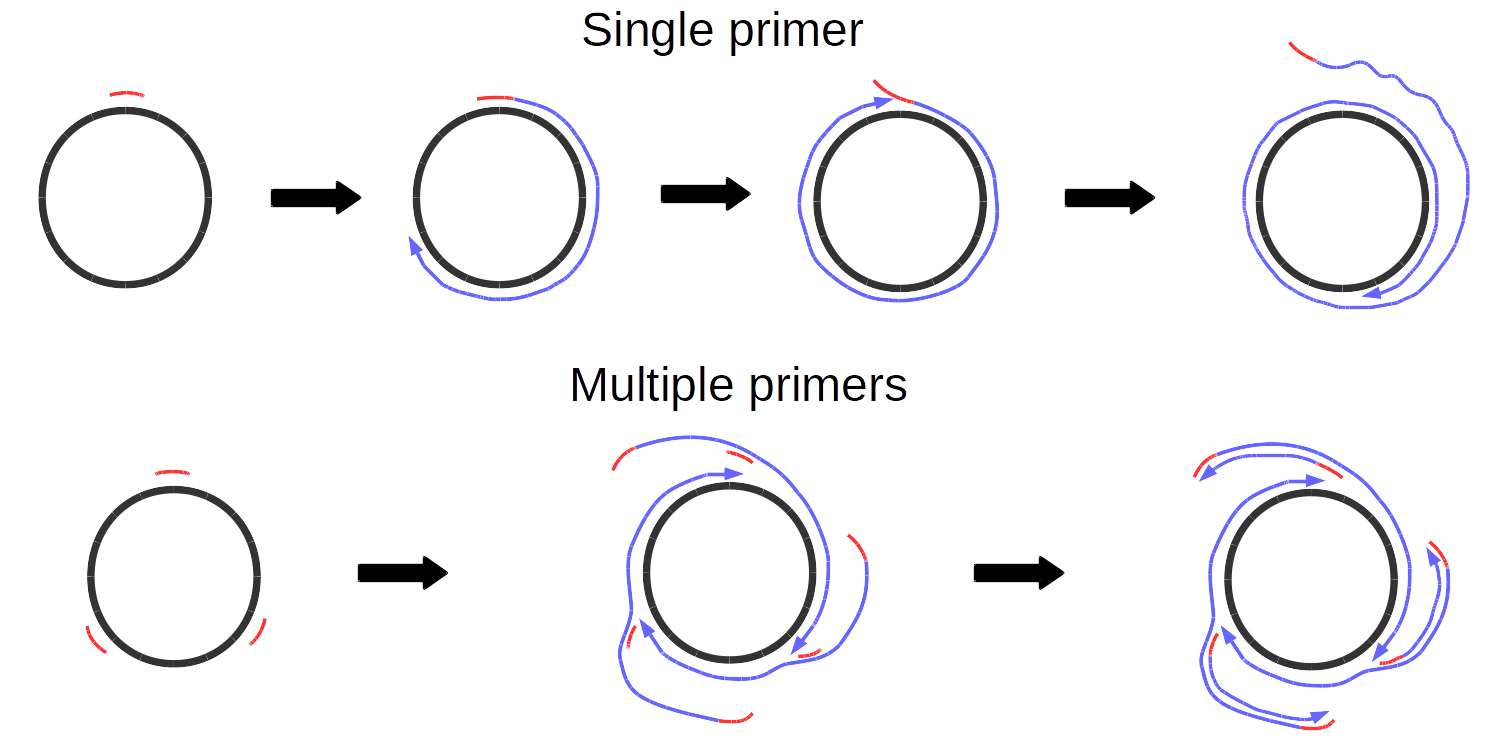
\includegraphics[width=0.9\textwidth]{images/rca.png}}
\caption[Rolling Circle Amplification]{General mechanism of Rolling-Circle Amplification. Figure is adapted from~\cite{Johne2009rca} (under Elsevier license number 4543471436155). Primer sequences are highlighted in red, the circular genome subjected for amplification is in black and the synthesized clones are in blue.}
\label{fig:concat_rca}
\end{figure}

The basic principle for RCA is shown in Figure~\ref{fig:concat_rca}~\cite{Johne2009rca}.
On top is an example of the process with only one imaginary primer binding to a template circular. The synthesis starts from this point and move across the whole length of the molecule in the complementary direction as being guided by the DNA polymerase  \emph{phi29} of bacteriophage \emph{Baccilus subtilis}.
Due to this particular enzyme's features, the incorporation can continue passing the binding site whilst the newly synthesized strand being displaced from the track.
Depending on the size of the template circle, the copying process can go several rounds, resulting in elongated molecules consisting of multiple copies of the original.
From the diagram in the bottom of Figure~\ref{fig:concat_rca}, multiple random primers are used for the amplification as it should usually be in practice. In this case, the abundance of primers from the reaction mixture can bind to the displaced strand and trigger additional syntheses, creating the branching patterns of the cloning process.

The RCA products are called concatemers as they are long concatemeric molecules consisting of consecutive copies of the target DNA sequence. Normally, restriction enzymes are used to chop them into separated monomers before taking further steps. For our method, concatemers are directly sequenced by MinION and computational methods are used afterward to detect such patterns.
\paragraph{Viral samples}
The viral genomes used in this study belonged to the plan infectious family \emph{Caullimoviridae}, or \emph{caulimovirids} with size varied around $7-9$ kpb.
Amongst nine genera detected~\cite{Geering2010ST,Mollov2013LZ}, two of them were investigated, namely \emph{Badnavirus} and \emph{Caulimovirus}, represented by \emph{Banana streak MY virus} (BSMYV) and \emph{Cauliflower mosaic virus} (CaMV) respectively.

\section{Bioinformatics analyses}

\subsection{Data description}
A multiplex sequencing has been conducted for 4 samples with the Rapid Barcode Sequencing kit. The barcode assignment is given in Table~\ref{tab:viral_samples}.
\begin{table}[!hpt]
\centering
\caption{Viral samples subjected to MinION barcoding sequencing}
\label{tab:viral_samples}
\begin{tabular}{|l|l|l|r|r|}
\hline
\textbf{Barcode} & \textbf{Sample} & \textbf{Description} & \textbf{Pass reads}  & \textbf{N50}    \\\hline
08                  & CaMV+              & \emph{Cauliflower mosaic} virus  &   14,385   &      6,707 \\\hline
09                  & BSMYV+             & \emph{Banana streak MY} virus    &   3,389   &   8,178   \\\hline        
10                  & BSMYV-             & \emph{Banana streak MY} virus, negative control     &   4,653   &  6,023   \\\hline
12                  & CaMV-              & \emph{Cauliflower mosaic} virus, negative control     &   9,942   &  4,919   \\\hline
\end{tabular}
\end{table}

\subsection{Reference-based detection of concatemers}
Raw signal data from MinION were base-called and demultiplexed by \albacore{} version 2.1.0. This resulted in 4 DNA sequence files corresponding to 4 barcoded samples, only pass reads from those sequences were used for further analyses.

\paragraph{Work flow} Due to the application of rolling circle amplification, each long read is expected to contain more than one copy of the virus DNA, potentially sitting next to each other in a \emph{concatemer}. We create an in-house pipeline to detect and extract the \emph{monomer} sequences out of the reads to build their consensus as shown in Figure \ref{fig:concat_ref_workflow}.

\begin{figure}[ht]
\centerline{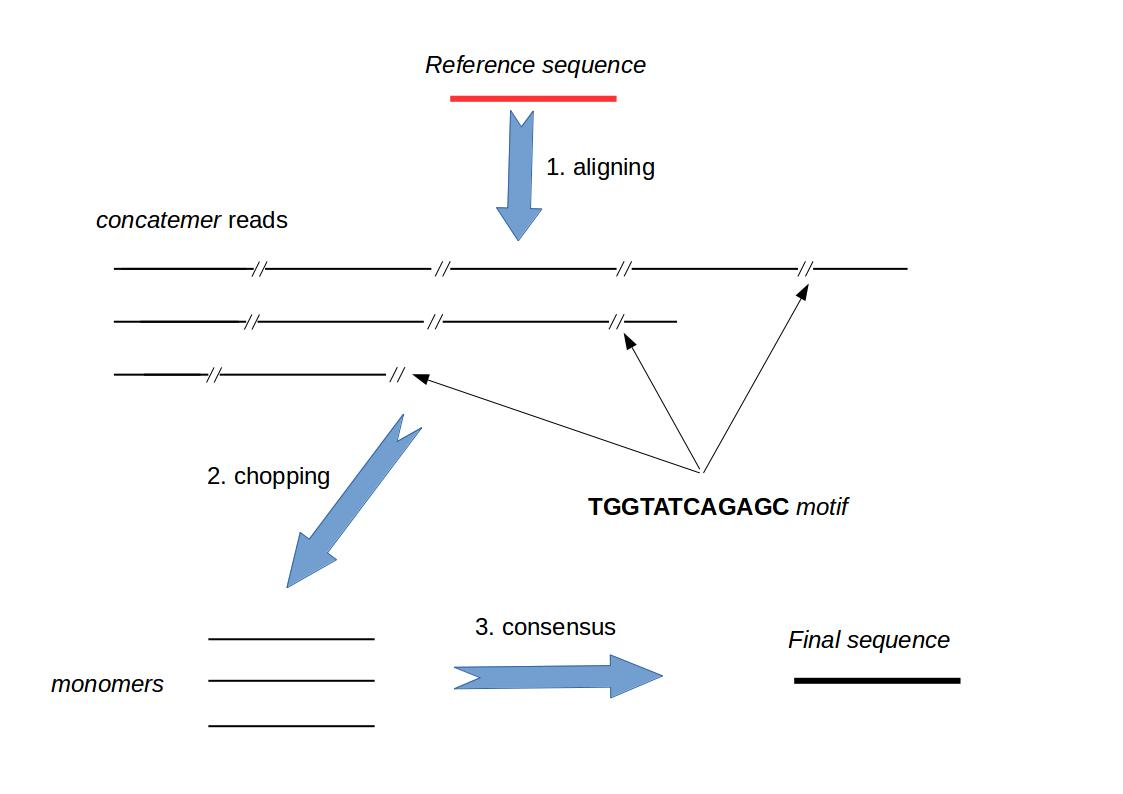
\includegraphics[width=0.9\textwidth]{images/concatemer.jpg}}
\caption{Pipeline to reconstruct viral genome sequences from MinION long reads.}
\label{fig:concat_ref_workflow}
\end{figure}

In more details, the pipeline is implemented in following the following steps: 
\begin{itemize}
\item[1.] align nanopore reads to the corresponding reference by \minimap{}~\cite{Li2016} version 2.11-r797 and keep only the ones covering $>80\%$ of the target; then induce locations of monomer on each reads based on the alignments.
\item[2.] for each monomer inferred, scanning for the nearest hit to the tRNA$^{Met}$ 12 nucleotides motif \textbf{TGGTATCAGAGC} of \emph{Caulimovirids}, then chop the read at those loci. %%COMMENT-LC sould explain why this motif 
\item[3.] build consensus sequence on those monomers by \racon{}~\cite{Vaser2017racon} version 1.2.1.
\end{itemize}

\paragraph{Align to the reference}
Figures \ref{fig:bc08} and \ref{fig:bc09} show the read length histogram of only mapped reads from nanopore data of barcode 08 and 09 respectively. Two negative control samples (barcode 10 and 12) returned no hits when aligned to their corresponding reference thus not shown. As can be observed, CaMV virus (barcode 08) has richer sequencing data compared to BSMYV sample (barcode 09).
\begin{figure}[!ht]
\centering
\subfloat[Mapped reads from barcode 08\label{fig:bc08}]{
	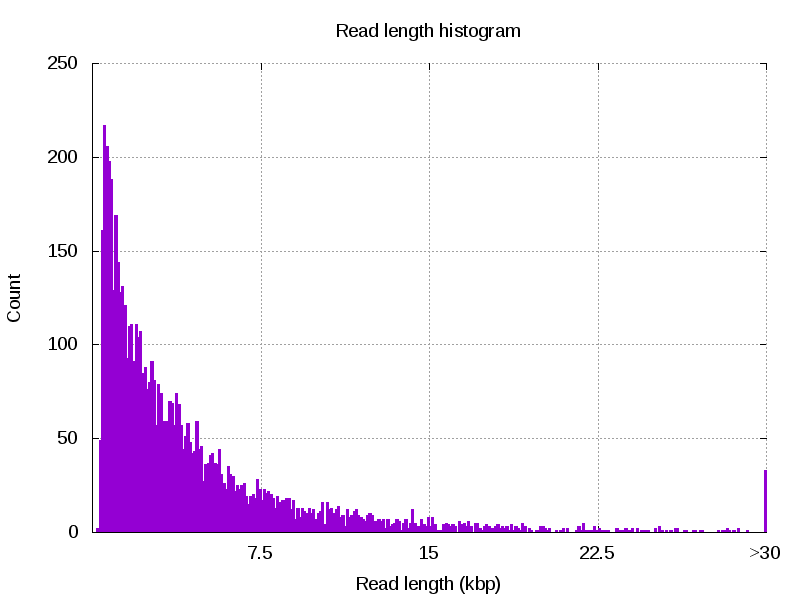
\includegraphics[width=.5\textwidth]{images/barcode08.png}
}
~
\subfloat[Mapped reads from barcode 09\label{fig:bc09}]{
	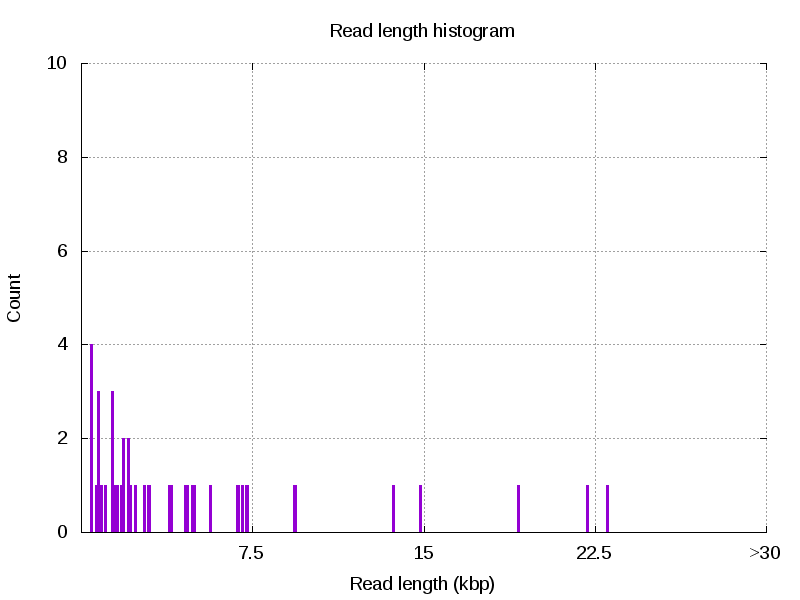
\includegraphics[width=.5\textwidth]{images/barcode09.png}
}
\caption{Mapped read length histogram of barcode 08 and 09.}
\label{fig:concat_map}
\end{figure}

\paragraph{Concatemer extraction}
Chart \ref{supp_fig:concat_count} presents the number of $k$-concatemers (concatemers with exact $k$ monomers extracted) for each positive sample (barcode 08 and 09). 
The longest concatemer detected was a 7-concatemer of CaMV DNA sequence. 
There was also one 6-concatemer and one 4-concatemer from this sample. 
In addition, the numbers of detected $k$-concatemers for \emph{Cauliflower mosaic} virus were more than 1 for $k=3$ (2 reads) or $k=2$ (6 reads).
Monomer reads made up the most abundance group with 33 CaMV sequences and 5 BSMYV sequences.
There were no other concatemers detected for the latter sample.

The extraction step generated in total $68$ and $5$-folds coverage of monomers respectively for barcode 08 and 09. By using these monomer sequences, we can pile them up and call the consensus sequence out of the nanopore data. The obtained sequence coverage played a critical role for the accuracy of the result: for barcode 08, the consensus was $99.5\%$ identical to its reference while it was only $93.72\%$ in case of barcode 09. 

\subsection{Reference-free method}
Assuming no references are given, the duplication of a DNA sequence in a nanopore read can still be detectable by using self-alignment to study the repeat pattern.
A proposed approach to investigate periodic repeat patterns is to use auto-correlation function (ACF) in digital signal processing (DSP) technique.
Similar DSP-based methods have been developed for fast biological sequence alignment and repeat detection \cite{Rockwood2005crosscorrelation,Ravi2007tandem}.
Here I present another application of signal processing techniques to detect the concatemers of the aforementioned viral sample using nanopore data. 
Tools are developed to work on both base-called and raw signal sequences.
For better demonstrating purpose, analysis result from the longest 7-concatemer read (from barcode 08 sample) is described without loss of generalization.

\subsubsection{Auto-correlation function}
Given an infinite sequence of discrete signals $S=\ldots s_1 s_2 \ldots s_k \ldots$ where $S(i)=s_i$ , its ACF $f(n)$ is defined as the cross correlation to itself
\begin{equation}
 f(n)=\sum_{k}{s_k\ast s_{k-n}}   
 \label{eq:acf}
\end{equation}
where $\ast$ operator returns a similarity score when compare two operands, \EG{} complex conjugate for $s(i) \in \mathbb{C}$~\cite{Rockwood2005crosscorrelation}, and $n$ stands for the lag value. By increasing this value, we have a sliding dot product between the signal vector with itself which in expect give peaks when repeat parts of the sequence are overlapped as demonstrated in Figure~\ref{fig:concat_acf}. Note that for every signal sequence $S$, there is always a peak at $n=0$ as a result from self-overlapping. In addition, the ACF values are symmetric with regard to this center value.
\begin{figure}[ht]
\centerline{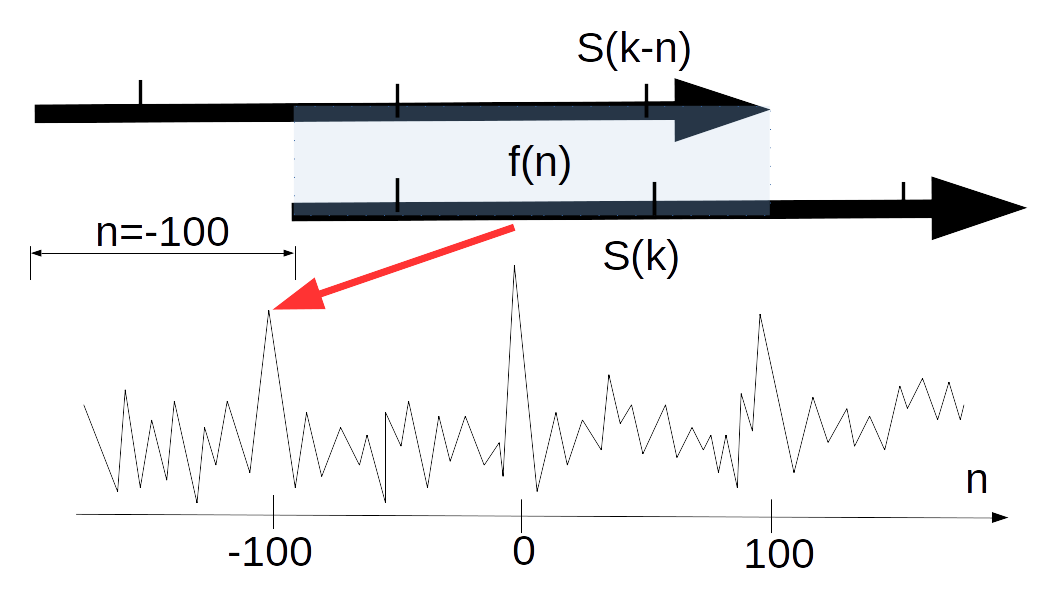
\includegraphics[width=0.7\textwidth]{images/acf.png}}
\caption[Example of ACF sliding dot product for a sequence with two repeats]{Example of ACF sliding dot product for a sequence with two repeats. The plots shows 3 dominating peaks corresponding to $n=-100, n=0, n=100$.}
\label{fig:concat_acf}
\end{figure}

In fact, the signal sequence to process is definite: $S=\{s_i\}, i=1 \ldots L$ for sequence with length $L$. Out of range values are normally zero padded $s_j \equiv 0 \: \forall j \leq 0,j > L$ or duplicated so that $s_i \equiv s_{i+n \times L} \: \forall n \in \mathbb{Z}$. In this study, the former filling method is used.

The following content will focus on ACF-based attempts in determining the concatemeric pattern of nanopore long reads.
Firstly, in the next section, a straightforward strategy will be employed  directly on the base-called sequence of nucleotides. The sliding dot product algorithm for the time-domain signal, together with a simple filter will be implemented initially. 
This simple but applicable method would serve as a proof-of-concept for the idea of using DSP technique to the problem.
After that, we introduce a more robust method that allows fast calculations not only on the DNA sequences, but also on the raw squiggle signals from the underlying ONT sequencing process. 
The ability to operate quickly per read would enable the concatemers detection to work in a streaming fashion so that it can be integrated in a real-time pipeline as aforementioned.

\subsubsection{Concatemers detection protocol using DSP}
To apply DSP algorithm, the first step is to convert the nucleotides sequence into appropriate digital signal.
Given a DNA sequence, we have $S(i)=s_i \in \{A,C,G,T\} \: \forall i \in \mathbb{N}$. A straightforward conversion is to map letters to their corresponding numerical values, \EG{} $\{1,2,3,4\}$ respectively.
Consequently, the $\ast$ operator from Equation~\ref{eq:acf} can be simply adapted to the Kronecker delta function
\[
s_i \ast s_j \equiv \delta_{s_i,s_j} = \left\{
\begin{array}{ll}
0     &  if \: s_i = s_j\\
1     &  if \: s_i \neq s_j
\end{array}
\right.
\]
As shown in Equation~\ref{eq:nkdf}, the ACF values are normalized by the overlap length to alleviate the position-dependant behaviour of the function that is important to locate peaks that represent monomer overlaps in next step. 
Due to the errors (indels/mismatches) of MinION sequence data, these overlaps are not aligned perfectly as of one-to-one mapping of base pairs but rather scattered hits along the overlapped region.
This results in a `group of nearby spikes' rather than a single prominent peak, making it more difficult to locate exact coordinates of monomers in the read. 
For that reason, a low-pass filter (LPF) is needed to help reduce the noises, or \emph{smooth} the signal before further analysis. 
Primarily, we use \emph{running average} with a fixed window size ($ws$) of nearby values for such task. 
We set the window size equal to 10 for this scenario. 

Overall, for this case, we investigate the signal of the normalized Kronecker delta function (NKDF) as shown in Equation~\ref{eq:nkdf}
\begin{equation}
\label{eq:nkdf}
f(n) = \frac{\displaystyle \sum_{i=1}^{L}{\delta_{s_i,s_{i-n}}}}
            {\displaystyle L-|n|}
            , n \in (-L;L)
\end{equation}
then apply the running average filter on it
\[
\overline{f(n)} = \frac{\displaystyle \sum_{i=-ws/2}^{ws/2}{f(n+i)}}
            {\displaystyle ws}
\]

\begin{figure}[!ht]
\centering
\subfloat[ACF for a random DNA sequence\label{fig:acf_random}]{
	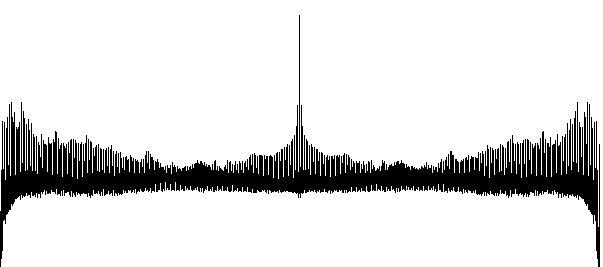
\includegraphics[width=.49\textwidth]{images/concatemer-random.png}
}
~
\subfloat[ACF for the 7-concatemer read\label{fig:acf_7cm}]{
	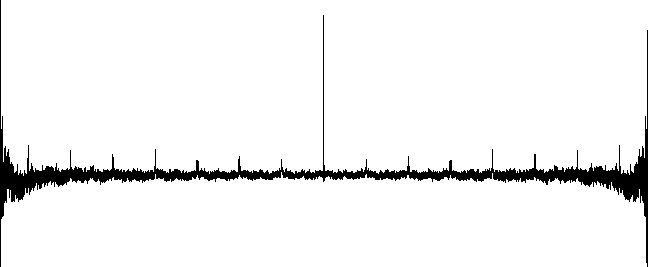
\includegraphics[width=.49\textwidth]{images/concatemer-7cm.png}
}
\caption{ACF values for a random read (\ref{fig:acf_random}) versus the 7-concatemer detected (\ref{fig:acf_7cm}).}
\label{fig:concat_acf_dna}
\end{figure}

Figure~\ref{fig:concat_acf_dna} presents the result signal for the detected 7-concatemer versus a random synthetic read with similar length.
According to the plots, there is only one distinct peak from the ACF signal of the random read which reflects the trivial case of self-alignment. On the other hand, from the longest concatemer read available, we can observe 7 clear peaks on each side of the symmetric squiggle representing the same copy number of the viral monomer.
These peaks are possibly identified by a peak picking algorithm which can determine the significant local maxima located across the range with similar distances. 

On the other hand, the formula \ref{eq:nkdf} implies greater variance of the signal values toward the ends of the range $(-L;L)$ due to fewer overlap data points involved. This tailing issue would hinders the algorithm to locate the monomers at two ends of a read. This effect can be observed from Figure~\ref{fig:acf_7cm} where the squiggles become more diverse leaving further the center lag ($n=0$).
For that reason, the peak picker will start the scan from $n=0$ to either side for distinct spikes of higher confident and determine the period before reaching the noisy peaks toward the ends.
Figure~\ref{supp_fig:concat_acf_dna} from the Appendix gives more examples of ACF-induced signals for several other $k$-concatemers using this calculation method. Similarly,  in all cases the fluctuations at the ends of ACF graphs are plotted beside the `genuine' maxima. This introduces difficulties to detect `real' hits close to the ends especially when $k=1$ as we have no other peak for comparison.

In general, via above experiment, the DSP approach utilizing ACF-based estimation has been proved to be feasible to detect the concatemeric pattern of nanopore RCA reads.
However, there are several points needed to be further developed and improved from this protocol to be able to work in an applicable pipeline.
The most important task is to optimize the algorithm to reduce the running time. The current sliding method takes $\mathcal{O}(L^2)$ time for a read of length $L$.
Even though it is relatively reasonable for viral concatemers of medium length ($\simeq 50$Kbp), it would become time-consuming to process reads with high copy numbers which are favoured and aimed for in this study.
Also, the turn-around speed per read is critical in real-time analysis, not to mention the desired application at the level of sequencing raw signal from the very pre-basecalling stage.
Another essential operation is a robust LPF mechanism since the simple moving average method is unable to comprehensively remove the high-frequency noises from the target signal. Lastly, a peak picking algorithm is needed to spot the periodical maxima and chop the repeat sequence at those breakpoints into monomers of interest.
All of those steps will be addressed in the following section.

\subsubsection{Rapid method to detect concatemeric signal}
\paragraph{Generalized problem for real signal data.}
While Kronecker delta function is fast to calculate, it is only suitable for sequences of discrete, categorical values \EG{} DNA letters. 
Nanopore raw signal for a read is given as a series of real values of electrical current sampled thousands times per second when the biological molecular transiting through the pore. 
Processing concatemers at raw signal level before base-calling would accelerate the whole pipeline to a new level, as well as improving the quality of signal for the next stage. 

From this context, the sequence $S,\: S(i)=s_i \in \mathbb{R} \: \forall i$ would have ACF written as
\[
 f(n)=\sum_{k}{s_{k}s_{k-n}}   
\]
where the $\star$ operator in Equation~\ref{eq:acf} is replaced by the multiplicity in $\mathbb{R}$ instead of the previous Kronecker delta function for discrete values of $\mathbb{Z}$.
Due to the symmetric property of ACF, only the right half of the range will be considered instead of the whole plot as demonstrated in Figure~\ref{fig:concat_acf_dna}, corresponding with lag from $0$ to $L-1$. The trivial peak of self-alignment thus locates in the very first element of the array.
\paragraph{Rapid estimation method for normalized ACF signal}
Calculation of ACF function given above is straight-forward and efficient using Fast Fourier Transform (FFT)~\cite{Gentleman1966FFT,Van1992FFT,Heideman1984FFT} with complexity $\mathcal{O}(L\log{L})$.
However, to additionally normalize the signal while maintaining the speed aspect of the algorithm is not a trivial task.
To achieve such goal, the Normalized Square Difference Function (NSDF)~\cite{Mcleod2005tartini} is implemented. This function can be calculated as shown in Equations~\ref{eq:nsdf}.
\begin{equation}
\label{eq:nsdf}   
\begin{array}{rr}
h(n)=& 1-\frac  {\displaystyle \sum_k{(s_k-s_{k-n})^2}}
                {\displaystyle \sum_k{(s_k^2+s_{k-n}^2})} \\
    =& \frac{\displaystyle \sum_{k}{2s_{k}s_{k-n}}}
            {\displaystyle \sum_k{(s_k^2+s_{k-n}^2})}\\
    =& \frac{\displaystyle 2f(n)}{\displaystyle g(n)}\\
\end{array}
\end{equation}
The values of $h(n)$ would fall in $(0,1]$ with $\forall n$, representing a normalized measure of proximity between $S$ and its $n$-delay signal. 

\begin{algorithm}[H]
\DontPrintSemicolon
\KwIn{Time-domain sequence signal $S$ of lenth $L$}
\KwOut{NSDF signal $H$}
\SetKwFunction{ACF}{ACF} 
\SetKwProg{Fn}{Function}{:}{}
\Fn{\ACF{$S$, $R$}}{ 
    $R:=\mathtt{fftForward}(S)$ \tcp*{Convert signal to frequency domain by FFT}
    $R[i]:=R[i] \star R[i]$, $\forall i=0 \ldots (L-1)$  \tcp*{complex conjugate every complex element}
    $R:=\mathtt{fftReverse}(R)$ \tcp*{Convert back to time domain by reverse FFT}
    \KwRet\;
}
\SetKwFunction{SS}{SS} 
\SetKwProg{Pn}{Function}{:}{}
\Pn{\SS{$S$, $M$}}{ 
    $SS[i]=S^2[i]$, $\forall i=0 \ldots (L-1)$ \;
    $M[0]=2*\mathtt{sum}(SS)$ \tcp*{get sum of all elements in $\mathtt{SS}$}
    $M[i]=M[i-1]-SS[i-1]-SS[L-i]$, $\forall i=1 \ldots (L-1)$ \tcp*{update incrementally}
    \KwRet\;
}
\Begin{
\ACF{S,R} \tcp*{calculate ACF and assign to R}
\ACF{S,M} \tcp*{calculate lag sum square and assign to M}
$H[n]=\frac{\displaystyle 2R[n]}{\displaystyle M[n]}$, $\forall n=1 \ldots (L-1)$ \tcp*{calculate NSDF as in Equation~\ref{eq:nsdf}}
\Return{$H$}
}
\caption{Algorithm to calculate the NSDF by using FFT.}
\label{algo:nsdf}
\end{algorithm}
More than that, this function is determined by $f(n)$ and $g(n)$ which can be both measured rapidly by using FFT (using $\mathtt{JTransform}$~\cite{Eichelberger2002jtransform}, a Java library for DSP) and incremental calculation as shown in Algorithm~\ref{algo:nsdf}.

\paragraph{LPF with Blackman windowing function.}
%http://www.labbookpages.co.uk/audio/firWindowing.html#windows
The plain moving average method is helpful to show the trend of the overall signal but not sensitive enough to completely remove the noises encountered.
Figure~\ref{supp_fig:concat_acf_raw} in the Appendix plots the NSDF of the 7-concatemer read with large smooth window sizes of $10,000$ and $20,000$. 
As a peak scanning method is sensitive to abundant of local optima, a `smoother' transition is expected via a signal filtering step. 
For that reason, a finite impulse response (FIR) filter by windowing is implemented.
\begin{figure}[!hpt]
\centering
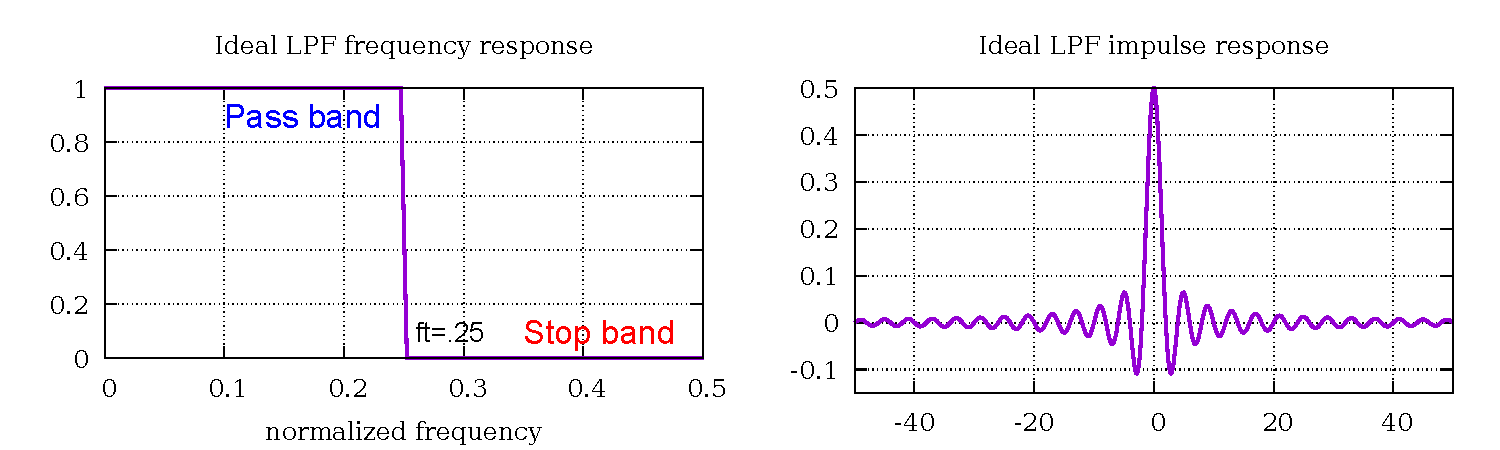
\includegraphics[width=\textwidth]{images/fir.pdf}
\caption{Example of ideal LPF at $f_t=0.25Hz$ and its corresponding impulse response.}
\label{fig:fir}
\end{figure}

Figure~\ref{fig:fir} gives example for an ideal LPS with transition (cutoff) frequency $f_t=0.25$. The left plot presents the frequency response of the filter in frequency domain (normalized with respect to the sampling frequency). In this perfect scenario, a brick-wall filtering is expected when any frequency values below $0.25Hz$ would pass and all higher components are stop.
This system would have an equivalent impulse response as shown on the right plot, given by function $\mathtt{IRF}$:
\[
\mathtt{IRF}(x) = 2f_{t}\ sinc(2\pi f_t x)
\]
where $sinc(x)$ is the \emph{sine cardinal} function
\[
sinc(x) = \left\{
\begin{array}{ll}
\frac{\displaystyle \sin{x}}{\displaystyle x}     &  if \: x \neq 0\\
1     &  if \: x=0
\end{array}
\right.
\]
In practice, to implement a finite impulse response LPF, only a window of the shifted sinc function is sampled for a finite number of filter weights. 
We set this window's length, or filter length, as the length of signal $L$. 
\begin{equation}
\label{eq:sinc}
\mathtt{IRF}(n) = \left\{
\begin{array}{ll}
\frac{\displaystyle \sin{[2\pi f_t (n-\frac{M}{2})}]}{\displaystyle \pi (n-\frac{M}{2})}     &  if \: n \neq \frac{M}{2}\\
2f_t     &  if \: n=\frac{M}{2}
\end{array}
\right.
\end{equation}
where $M$ is the filter order, defined as $M=L-1$.

Furthermore, to reduce the ripple from the ringing artifact due to crude approach of truncating the infinite ideal impulse response~\cite{Smith1997DSP,Bankman2008image}, we apply Blackman windowing~\cite{Harris1978use,Blackman1958measurement} instead of a rectangle window ($w(n)=1$) on the IRF values.
\begin{equation}
\label{eq:windowing}
w(n)=0.42-0.5\cos{\frac{\displaystyle 2\pi n}{\displaystyle M}}+0.8\cos{\frac{\displaystyle 4\pi n}{\displaystyle M}}
\end{equation}
Overall, to apply the LPS with Blackman windowing on the NSDF signal, we follow the steps below.
\begin{itemize}
    \item[(1)] Calculate the weights of the LPF as a function of cutoff frequency $f_t$ as in Equation~\ref{eq:sinc}
    \item[(2)] Multiply the result with the windowing calculated in Equation~\ref{eq:windowing}
    \item[(3)] Apply FFT for the result filter values.
    \item[(4)] Calculate FFT of the NSDF and multiply its values element-by-element to the filter values in the frequency domain.
    \item[(5)] Calculate the reverse FFT to get the result in the time domain.
\end{itemize}


The cutoff frequency (before being normalized) is empirically set as $100Hz$ assuming that a $100$-times RCA duplication is virtually impossible or due to process's artifacts.
This threshold can be set more stringent with knowledge about specific reference genome size and obtained sequencing read length. 
Figure~\ref{fig:mpm100} shows the filtered signals for the only $7$-concatemer read, at both pre- and post- base-calling stage. 
Additionally, Appendix Figure~\ref{supp_fig:mpm30} depict plots from applying the method with cutoff frequency of $30Hz$.
As expected, the signal will become `smoother' as the transition frequency decreased but would risk the specificity of the signal and generalization of the method when apply to other data set.
The filtered signal is now ready to be used as input for a pick peaking method to detect the repeat pattern of the concatemeric reads.
\begin{figure}[!hpt]
\centering
\subfloat[DNA sequence\label{fig:mpm100_dna}]{
	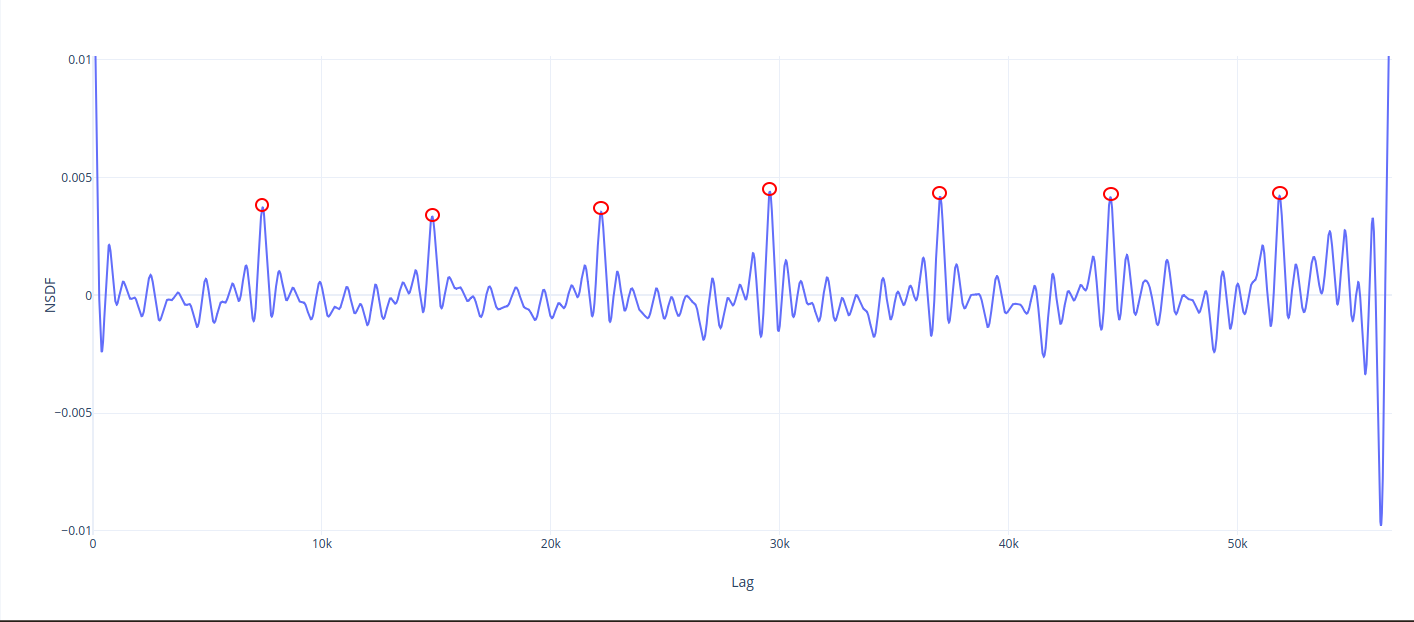
\includegraphics[width=.9\textwidth]{images/nsdf-dna-cut100.png}
}
\\
\subfloat[Raw signal\label{fig:mpm100_raw}]{
	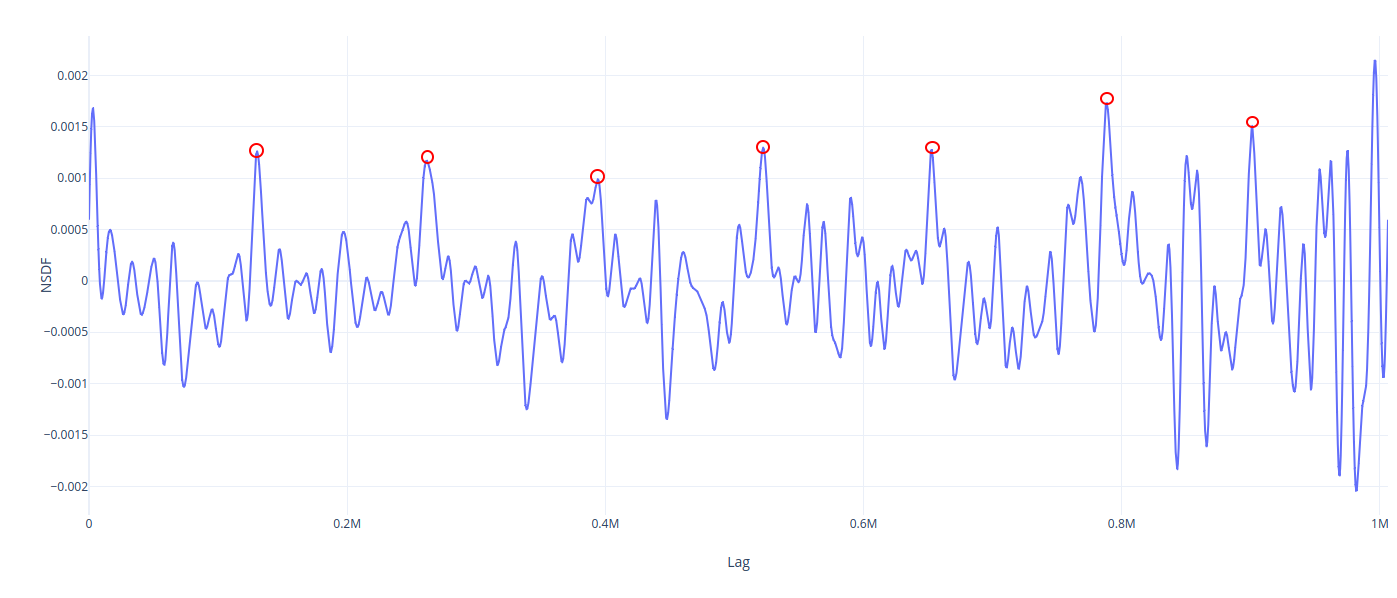
\includegraphics[width=.9\textwidth]{images/nsdf-raw-cut100.png}
}
\caption[Peak picking for a 7-concatemers NSDF signal processed with LPF using $cutFreq=100$]{Peak picking results for a 7-concatemers NSDF signal processed with LPF using $cutFreq=100$ of (\ref{fig:mpm100_dna}) the base-called DNA sequence and (\ref{fig:mpm100_raw}) its corresponding raw signal.}
\label{fig:mpm100}
\end{figure}

\paragraph{Pick peaking algorithm}
A list of candidates are first selected out of all local maxima by choosing the highest ones locating between every positively sloped zero crossing and negatively sloped zero crossing~\cite{Mcleod2005tartini}.
By setting the cutoff frequency, a respective minimum period (or monomer length) is determined as a consequence: $minLen=\frac{\displaystyle 1}{\displaystyle cutFreq}$. 
Any peaks on the left of this value will be ignored and the algorithm will iteratively scan to the right in the remaining peaks list for the correct first peak.
The correct first peak at $n_1$ must satisfy criteria as below:
\begin{itemize}
    \item[(1)] There are at least $\lfloor \frac{\displaystyle L}{\displaystyle n_1} \rfloor - 1$ more peaks with similar distances along the signal sequence.
    \item[(2)] The sum of these peaks' height must be more than a certain portion, \EG{} $0.8$, of the counterpart for all candidates.
\end{itemize}
The algorithm will stop at the very first coordinate that meets above 2 conditions and return the list of periodic peaks which can be used to break the concatemer into monomers. 

Figure~\ref{fig:mpm100} also reflects the peak-picking results applied for the longest concatemeric read. 
In both signal level, we detect exactly 7 peaks (highlighted in red dots) corresponding to the breakpoints that can be used for a $7$-concatemer chopping process.
Interestingly, when the peaks from DNA signal shows very stable repeat pattern, there is a slight variance from raw signal toward the far end. 
This phenomenon is shown clearer in Appendix Figure~\ref{supp_fig:mpm30_raw} when the sixth peak is shifted more to the right, considerably making the sixth monomer longer and the seventh monomer shorter than average.
We argue that there should be an unsmooth transition of the squiggle signal reading from the sequencing process~\cite{Rang2018squiggle}.
This is due to the nonuniform translocation time of the DNA molecule caused by the motor enzyme at the \emph{homopolymeric} regions~\cite{Manrao2012reading,Cherf2012automated,Sarkozy2017calling} and normally responsible for the high indel error from nanopore sequencing~\cite{Jain2018nanopore3,Stancu2017nanopore5,Ip2015minion}.
However, the base-calling in this case has successfully manipulated the situation, resulting in more evenly-distributed peaks being detected.

Overall, via above example, we demonstrated that a 7-concatemer can be detected using the reference-free method based on NSDF signal investigation.
Similarly, any $k$-concatemer ($k \geq 1$) can be identified by the same manner and its monomers can be extracted by chopping at respective break-points. However, in order to obtain results of high confident, only reads corresponding to $k \geq 2$ should be selected as they would show more than 2 peaks for an affirmative picking task.
\section{Conclusion}
This chapter demonstrated a method of using MinION sequencing together with RCA for small-sized circular genomes, in particular two samples from \emph{Caulimovirids}.
Results from this preliminary finding showed that concatemer molecules generated from RCA can be sequenced directly by the thumbnail sequencer without using restriction enzymes to physically divide them into monomers. 

In fact, this step can be accomplished by using computational approaches, given or not a reference sequence.
In the reference-based method, corresponding monomers' break-points for RCA reads could be detected straightforward, resulting in abundance of single-copied sequences that could be subjected to a consensus calling.
For the \emph{de novo} detection algorithm, concatemeric reads were more confidently identified if they contains higher number of monomer duplication. For that reason, we can apply the reference-free method on data from CaMV barcoded sample to extract monomers and run the consensus calling with 35-folds coverage. RCA for BSMYV, on the other hand, returned solely monomers which were exclusively detectable given the reference DNA.
Further improvement from sequencing phase should be made in order to achieve longer stretches of clones so that the pipeline can operate completely without prior knowledge about the target genome.

The implemented module could operate rapidly read-by-read thus it is able to adapt for a streaming pipeline. For instance, a viral or plasmid sequencing would run until sufficient copies of monomers are produced for each sample.
Furthermore, the whole process can be established at raw signal level, before the base-calling step. 
For reference-based algorithm, the alignment step can be carried out between sequences of squiggle signal, as described in \emph{Read-Until} protocol~\cite{LooseMS2016}.
In case a reference is not provided, an DSP implementation based on NSDF is available for the task of determining concatemers.

In summary, this approach provide another promising method to study relative small but highly varied genomes of microorganisms. For instance, the longer concatemeric sequences will offer superior resolution to the nucleotides of individual virus thus enhancing the knowledge about inter- and intra-sample variations of this rapid evolving species. Continuing efforts are made to improve the monomer copy numbers from RCA reads so that we can utilize the methods in more comprehensive ways for real-life applications.

%%%%% Conclusion
\cleardoublepage
\chapter{Conclusion}\label{ch:conclusion}
\thispagestyle{empty}
\vspace*{\fill}
\epigraph{\emph{In the end we come up with a conclusion that we need to start from somewhere.}}
{--Deyth Banger}

\clearpage
%%%%%%%%%%%%%%%%%%%%%%%%%%%%%%%%%%%%%%%%%%%%%%%%

\section{Thesis summary}
The advent of Third-generation sequencing methods, particularly ONT platforms, have brought novel opportunities together with challenges to the field of bioinformatics similar to those arisen from the arrival of Second-generation sequencing methods before ~\cite{SchadtTK2010,ThkurRB2012}.
Chapter~\ref{ch:intro} has provided a brief review as well as comparison between these two generations of sequencing methods, aiming at their applications in genome assembly.
Specifically, the long spanning reads generated in real-time from ONT MinION device had been found to be useful in generating more complete assemblies despite of their error profiles~\cite{GoodwinGE2015,MadouiEC2015,Karlsson2015}. 

Throughout this thesis, computational methods have been designed and applied to complete genomes as fast as possible.  
For that purpose, Chapter~\ref{ch:npscarf} described \npscarf{}, a streaming hybrid assembler that could finish the fragmented short-read assemblies using the consecutive nanopore reads. In addition, we have shown that the pipeline could be used to determine the locations of highlighted genes of interests on the whole genome during its construction in real-time.
To adapt the parallel mechanism of MinION using barcode sequencing in our streaming pipelines, \npbarcode{} has been developed and its applications were mentioned in Chapter~\ref{ch:npbarcode}. The scalability of \npscarf{}, as well as of other streaming analyses, to multiple samples were verified through this chapter.
Chapter~\ref{ch:npgraph}, on the other hand, focused on designs to help improve the accuracy of the assembly output. This resulted in \npscarf{}\_wg and especially \npgraph{} which employed the assembly graph for better fidelity.
Lastly, Chapter~\ref{ch:concatemers} conducted computational analysis on the MinION data of concatemeric long reads in an attempt to produce viral genome assembly in an efficient way.

\section{Key contributions}
Overall, the thesis focuses on genome assembly methods using the MinION data and how to exploit its real-time feature to reduce the turn-around time of the computational analyses.
Accordingly, the main contributions fall into two categories as followed.
\paragraph{Contributions to genome assembly methods}
We offered a set of open-source software and utilities for genome assembly using Nanopore data.
In combination with short-read assemblies, \npscarf{} can finish and return complete genomes in a short amount of time while consuming less resources compared with other methods.
In addition, \npbarcode{}, a robust multiplexer for barcode sequencing, can be used together with \npscarf{} to scaffolding multiple samples at the same time.

We also addressed an use case of using a combination of \npscarf{} with other prominent methods consuming the same inputs. Through this example, ones can measure the advantages and disadvantages of each method to come up with the best solution possible.
Importantly, if short-reads assembly graph is provided, \npgraph{} can be employed for more accurate results. It also comes with a GUI to monitor the process in an user-friendly manner.

Finally, we proposed another assembly method for small circular genomes using concatemeric MinION reads after RCA. Either a reference-based or reference-free assembly algorithm can be applied on the long reads to generate the monomers of whole genome sequences with decent quality given sufficient read coverage.
\paragraph{Contributions to real-time analysis}
To date, \npscarf{} and its derived version \npgraph{} are the only assembly methods exclusively designed to assemble genomes in real-time in accordance with MinION's output.
We have successfully addressed, implemented and applied a streaming pipeline to rapidly finish short-read assemblies using real-time sequencing.
As a result, it enabled real-time analyses that rely on positional information, including but not limited to identifying genes encoding bacterial genomic islands and plasmids.
These functional regions in the bacterial genomes can be horizontally transferred between organisms, which is one of the main mechanisms for acquiring AMR in pathogenic bacteria.  

Furthermore, the streaming demultiplexer \npbarcode{} allows the pipeline to run in parallel for multiple samples.
This feature is critical to clinical applications such as diagnosis and treatments, especially in emergency units, which normally require quick response from multiple testing activities.
On the other hand, the ability to operate and to monitor completion status in real-time (even with GUI) allows users to decide when to stop the sequencing process thus fulfilling the task of saving time and cost for genome analyses.
The reference-free concatemeric assembler from Chapter~\ref{ch:concatemers} can even work with raw signal from the sequencing device hence open up the possibility to be integrated into the \emph{ReadUntil} pipeline~\cite{LooseMS2016} which had been designed to further reduce the turn-around time of the nanopore data analyses.
\section{Future directions}
\paragraph{Improve software performance}
The thesis has shown continuous development of a real-time hybrid assembler. It has evolved from the original \npscarf{} to a version with assembly graph (\npscarfg{}) and ultimately an exhaustive graph-traversing algorithm (\npgraph{}). 
The efforts indeed have leveled up the accuracy of the assembly output considerably.
Even though, there are still rooms to enhance the performance of the software given the inputs kept intact.
Specifically, there is a need for more robust voting system and/or a decision making mechanism to be able to determine bridges with higher confidence in real-time.  
Other than that, a revertible bridge construction on the graph is also considered for a self-rectifying assembly mechanism of \npgraph{}. 

\npscarf{}, on the other hand, performs better with mid- or large-size data sets. However, an optimization is required to minimize the resources required when working with huge and complicated genomes, \EG{} of eukaryotic organisms.
Besides, \npscarf{} and \npgraph{} are currently working as two separate modules due to different methodology and implementation. For convenience, they will be integrated in one common interface of a hybrid assembly software supporting different scenarios.

\paragraph{Application in metagenomics}
Preliminary works on mock data sets of metagenomics using \npscarf{} have demonstrated that our approach is feasible for this case (data not shown).
As a consequence, one of the development direction is to implement a hybrid assembler that can solve metagenomics assembly graph in real-time with \npgraph{}.

In order to achieve this, we first plan to run \spades{} with $\mathtt{--meta}$ option~\cite{Nurk2017metaspades} to generate a metagenomics assembly graph. After that the contigs (nodes from the graph) will be subjected to a binning algorithm, \EG{} $\mathtt{metaBAT}$~\cite{Kang2015metabat}, to discover the populations of the community.
This information is then used to determine multiplicity and membership of each contigs so that \npgraph{} algorithm can work with and produce assembly for each of those detected populations.

\paragraph{Non-hybrid methods}
It is desired to have a non-hybrid real-time \emph{de novo} assembly as the yield and quality of the nanopore reads being generated are increased significantly compared to the early stage. 
In fact, there are several fast algorithms being developed recently for such task in batch-mode, \IE{} $\mathtt{miniasm}$~\cite{Li2016} or $\mathtt{wtdbg2}$ (Ruan, J. and Li, H. (2019) \emph{Fast and accurate long-read assembly with wtdbg2}. bioRxiv. doi:10.1101/530972).
However, to adapt those approaches for a streaming pipeline is non trivial.
The modified OLC or DBG algorithm for nanopore data are both consuming much more resource due to the errors.
Furthermore, the error correction step, \EG{} $\mathtt{racon}$~\cite{Vaser2017racon} using POA graph data structure, is costly thus make it difficult to operate in real-time during the sequencing process.
\section{Closing remarks}
Long-reads data from TGS platforms, such as MinION, are considered as the  current game-changer for genomics studies, especially genome assembly which has been partly addressed throughout the thesis.

Recently, however, there has been arguments concerning the quality of long-reads assembly from the DNA reference resource, such as NCBI database, that would affect the downstream analyses at protein level due to relatively high error rates especially indels~\cite{Watson2019errors,Koren2019reply}.
In the meantime, the hybrid approaches can combine the high fidelity of sequence data from Illumina to overcome the current defects of TGS assembly.
Plus, the innovation of technology in combination with the improvement of computational methods can leverage the genome assembly for not only microorganisms, but also human and multiploidy species of greater complexity.

To sum up, the author strongly believe that the long reads real-time sequencing methods, \EG by using ONT platforms, and their applications  will continue to be the trending direction in life science. 
Advancements made by scientific and commercial bodies in this field would greatly facilitate the genome sequencing practice in order to ultimately resolve the long-lasting assembly problem.



%%%%% Bibliography, in BibTeX format (the .bib file)
\cleardoublepage
\bibliography{bib/all}

\cleardoublepage
\begin{appendices}
\newcommand{\nocontentsline}[3]{}
\newcommand{\tocless}[2]{\bgroup\let\addcontentsline=\nocontentsline#1{#2}\egroup}
\fancyhf{}
\fancyhead[LE,RO]{\nouppercase{\thepage}}
\fancyhead[LO]{\sc \nouppercase{Appendices}}
\fancyhead[RE]{\sc \nouppercase{Appendices}}

\addtocontents{toc}{\protect\setcounter{tocdepth}{ 0}}
\chapter{Supplementary materials for Chapter 2}\label{app:npscarf}
%\addtocontents{toc}{\protect\setcounter{tocdepth}{ 0}}
%\addcontentsline{toc}{chapter}{Appendix \thechapter}

\newpage

\begin{figure}[!hpt]
\centering
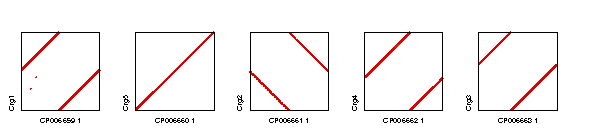
\includegraphics[width=15.84cm]{images/suppFigure1.pdf}
\caption[Alignment of the \npscarf{}'s assembly for \kp{} ATCC BAA-2146 to its reference genomes]{Alignment of the \npscarf{}'s assembly for \kp{} ATCC BAA-2146 to its draft
reference genomes (GeneBank Accession GCA\_000364385.2). The five contigs were
in complete agreement with the chromosome and four plasmids.}
\label{SF:alignKp2146}
\end{figure}

\begin{figure}[!hpt]
\centering
\includegraphics[width=9.76cm]{images/suppFigure2.pdf}
\caption[Alignment of the \npscarf{}'s assembly for \kp{} ATCC 13883 to its reference genomes]{Alignment of the \npscarf{}'s assembly for \kp{} ATCC 13883 to its draft
reference genomes (GeneBank Accession GCA\_000742135.1). 
For display convenience, IDs of reference sequences are abbreviated by the last two digits
before the dot in the original accession code: 
Contigs 1 and 2 were aligned to the reference Scaffold 18 (KN046818.1). 
Contig 4 was aligned to two Scaffolds 19 (KN046819.1) and
22 (KN046822.1) and Contig 3 to Scaffolds 20 (KN046820.1) and 21 (KN046821.1).}
\label{SF:alignKp13883}
\end{figure}


\begin{figure}[!hpt]
\centering
\includegraphics[width=19cm]{images/suppFigure3.pdf}
\caption[Alignment of the  \npscarf{}'s assembly for \sce{} W303 to the reference
genome of the S288C strain]{Alignment of the  \npscarf{}'s assembly for \sce{} W303 to the reference genome of the S288C strain. Ten chromosomes (II, IV, V, VII, IX, X, XI, XIII, XV, XVI and the mitochondrion) were constructed into individual contigs, three chromosomes (I, III and VIII) were into two contigs each, and three chromosomes (VI, XII and XIV) were fused into two contigs because of mis-assembly.}
\label{SF:alignW303rt}
\end{figure}


\begin{figure}[!hpt]
\centering
\includegraphics[width=19cm]{images/suppFigure4.pdf}
\caption[Alignment of the Canu's assembly for \sce{} W303 to the reference
genome of the S288C strain]{Alignment of the Canu's assembly for \sce{} W303 to the reference genome of the S288C strain.  Chromosomes II and XVI were fused onto three
contigs.
}
\label{SF:alignW303Canu}
\end{figure}


\begin{figure}[!hpt]
\centering
\includegraphics[width=19cm]{images/suppFigure5.pdf}
\caption[Alignment of the miniasm's assembly for \sce{} W303 to the reference
genome of the S288C strain]{Alignment of the miniasm's assembly for \sce{} W303 to the reference genome of the S288C strain. Chromosomes V and XI were fused onto three contigs.}
\label{SF:alignW303Min}
\end{figure}

\clearpage

Supplementary Table~\ref{T:mem} shows the memory usage of the tools on
the datasets described in the paper. The scaffolders (SSPACE, LINK and
\npscarf{}) were run on the short read assemblies outputed by SPAdes. We hence
only present the memory footprint from running these tools only. The memory
requirement for each pipeline should be the \emph{maximum} between memory usage
of the tool and SPAdes. For NaS and Nanocorr, the error correction steps were
distributed across hundreds of jobs, each consumed a small memory footprint. We
report here only the memory usage from running  The values reported in the table
were from running Celera Assembler. Note that we ran Celera Assembler on
differing configurations, and we reported the here the memory usage of the
configuration resulting in the most complete assembly.
Memory reported for Canu and Miniasm was the \emph{maximum} among all tasks
in the pipeline (including Pilon and BWA-MEM) because each task can be run one
at a time; However, the reported memory usage for \npscarf{} was the \emph{sum} of 
memory for running \npscarf{} and BWA-MEM.
\begin{table}[!hpt]
\centering
\caption{Memory usage (Gb) of the different tools}
\label{T:mem}
\begin{tabular}{lrrrrrrrrrr}
% \toprule
%    &       & \cthead{1}{Assembly} & \cthead{1}{\#Contigs}      & 
%    \cthead{1}{N50}  & \cthead{1}{Mis-} &  \cthead{1}{Error}  &
%    \cthead{3}{Runtimes} \\
%    & Method & \cthead{1}{size (Mb)} &\cthead{1}{($\geq500$ bp)} &
%    \cthead{1}{(Kp)} & \cthead{1}{assemblies} & \cthead{1}{(per 100 Kb)} &  
%    \cthead{3}{(CPU hrs)} \\
\toprule
 & Kp2146 & Kp13883 & E.coli K12 & ST H58 & Sc W303\\
\hline
SPAdes & 35.67 & 34.32 & 34.24 & 10.45 & 85.99 \\
 + SSPACE & 3.41 & 4.01 & 5.09 & 2.39 & 36.84 \\
 + LINK & 28.47 & 16.33 & 44.83 & 19.89 & 233.49 \\
 + \npscarf{}{} (rt) & 2.11 & 1.11 & 2.32 & 1.27 & 4.27\\
% + \nname{} (b) & 0.67 & 0.62 & 0.62 & 0.62 & 2.37 \\
NaS + CA & 8.02 & 8.10 & 9.21 & 8.23 & 83.60 \\
Nanocorr + CA & 3.76 & 3.99 & 6.91 & 1.57 & 159.91 \\
Canu + Pilon & - & 6.78 & 6.30 & - & 56.20 \\
Miniasm + Pilon & 2.99 & 6.08 & 6.04 & 1.97 & 89.51 \\
\hline
\end{tabular}
\end{table}

\addtocontents{toc}{\protect\setcounter{tocdepth}{ 0}}
\chapter{Supplementary materials for Chapter 3}\label{app:npbarcode}
%\addtocontents{toc}{\protect\setcounter{tocdepth}{ 0}}
%\addcontentsline{toc}{chapter}{Appendix \thechapter}
\newpage

\begin{figure}[!hp]
\includegraphics[width=\textwidth]{images/vntr1.png}  
\caption[PCR barcode MinION sequencing with \npbarcode{}]
{Another application of \npbarcode{} with GUI for ONT sequencing using PCR barcoding kit (3 libraries, Albacore base-caller).}
\label{supp_fig:npbarcode_pcr}
\end{figure}

\begin{table}[!htb]
\caption{Information for each of 8 samples used in the Native Barcoding sequencing protocol.}
\label{supp_tab:sample}
\centering
\begin{tabular}{l|l|l|l|r}
\textbf{ID} & \textbf{Strain}          & \textbf{Publish ID} & \textbf{Barcode ID} & \textbf{Input (ng)} \\\hline
GP\_023            & \emph{Streptococcus pneumoniae} &        ATCC 700677              & NB01                & 1,000                \\
GN\_092            & \emph{Klebsiella pneumoniae}    &         3\_GR\_13~\cite{Miranda2018}             & NB02                & 1,500                \\
GN\_093            & \emph{Acinetobacter baumannii}  &          n/a            & NB03                & 1,500                \\
GN\_096            & \emph{Klebsiella pneumoniae}    &         5\_GR\_13~\cite{Miranda2018}              & NB04                & 935                 \\
GN\_101            & \emph{Pseudomonas aeruginosa}   &          n/a            & NB05                & 1,500                \\
GN\_106            & \emph{Klebsiella pneumoniae}    &         11\_BR\_13~\cite{Miranda2018}              & NB06                & 1,500                \\
GN\_132            & \emph{Klebsiella quasipneumoniae}    &         21\_GR\_13~\cite{Miranda2018}              & NB07                & 1,000                \\
GN\_133            & \emph{Klebsiella pneumoniae}    &         22\_GR\_12~\cite{Miranda2018}              & NB08                & 1,500               
\end{tabular}
\end{table}

% From the native sequencing, we also run Porechop and poreFUME, together with Metrichor's demultiplexer for comparison. It is worth noting that since Metrichor's demultiplexer only works on 2D sequencing reads for the time we conduct the experiment, it is  therefore necessary to limit the comparison within this set.

% Each demultiplexer's output is a set of read bins where each bin is supposed to correspond to one target library. To evaluate the accuracy of the classification, we align all reads back to the references by BWA-MEM. Theoretically to be the absolute ground truth, every single read must align to exact one reference. However, this is not the case due to nanopore sequencing error rate (causing no hit found) and the similarity between 8 bacterial samples in use (causing confusions because of multiple and/or chimeric hits). 

\begin{table}[!hp]
\centering
\caption[Pairwise comparison between samples in Native Barcode Sequencing]{Pairwise comparison (using MUMmer) between 8 samples in our Native Barcode Sequencing. Value in cell $(i,j)$ is percentage (bases) of genome $i$ aligned to genome $j$. Highly identical genomes and their figures are highlighted.} 
\label{supp_tab:dnadiff}
\begin{tabular}{l|llllllll}
\hline
& GP\_023 & \textbf{GN\_092} & GN\_093 & \textbf{GN\_096} & GN\_101 & \textbf{GN\_106} & \textbf{GN\_132} & \textbf{GN\_133} \\ \hline
GP\_023 & 100 & 0.30 & 0.16 & 0.27 & 0.09 & 0.34 & 0.28 & 0.30 \\
\textbf{GN\_092} & 0.14 & 100  & 0.30 & \textbf{87.28} & 1.09 & \textbf{92.74} & \textbf{78.42} & \textbf{97.11} \\
GN\_093 & 0.13 & 0.32  & 100 & 0.32 & 0.30 & 0.25 & 0.23 & 0.3  \\
\textbf{GN\_096} & 0.14 & \textbf{88.84}  & 0.31 & 100 & 1.27 & \textbf{88.10}  & \textbf{79.75}  & \textbf{86.24}  \\
GN\_101 & 0.03 & 0.90 & 0.15 & 1.00 & 100 & 1.02 & 0.73  & 0.72 \\ \textbf{GN\_106} & 0.17  & \textbf{93.96} & 0.17 & \textbf{87.47} & 1.19  & 100 & \textbf{79.65} & \textbf{91.86}  \\
\textbf{GN\_132} & 0.13 & \textbf{79.99}  & 0.16  & \textbf{79.94} & 0.84 & \textbf{80.50} & 100 & \textbf{79.66} \\
\textbf{GN\_133} & 0.15 & \textbf{99.99} & 0.26 & \textbf{87.31} & 0.93    & \textbf{93.47} & \textbf{80.50} & 100 \\ \hline
\end{tabular}
\end{table}

% \tab{tab:dnadiff} shows the intersection of those genomes in pairs. From the table, 5 out of 8 samples shares significant identical genome's content. Especially there are three bacteria namely GN\_092, GN\_106 and GN\_133 possessing more than 90\% identity thus rooting great possibility of confusing alignments. On the other hand, 3 out of 8 genomes are  significantly unique when only sharing around 1\% or less of common bases to another. In fact, the only gram negative species GP\_23 is the most diverged isolate amongst all.

% Despite of aforementioned issues, for the comparison purpose, we can still have a decent estimation on the accuracy of the binning algorithms based on alignment. We extract the best out of all possible alignments for a read and assign its origin as the best-hit reference. Results are shown in \fig{fig:comparison}. For better illustration, divergences between samples are reflected via corresponding color palette, e.g. GN\_092, GN\_106 and GN\_133 are filled with nearly identical colors due to their highly similarity.

\begin{figure}[!hpt]
\includegraphics[width=\textwidth]{images/alignment.png}
\caption[Comparison of ONT Native Barcode Sequencing demultiplexing accuracy]
{Comparison of ONT Native Barcode Sequencing (8 libraries) demultiplexing accuracy. The bars present the number of aligned reads to references. Each group of bars correspond to a demultiplex bin. Bars in a group, from left to right, are from (1) the total data set (2) \npbarcode{} (3) Porechop (4) poreFUME demultiplex. GN\_092, GN\_106, GN\_133 together with GN\_096 and GN\_132 are very close thus being filled by similar colors (pink-red).}
\label{supp_fig:comparison}
\end{figure}

% In general, the performances of 4 demultiplexers are stably comparable, especially \npbarcode{}, Porechop and Metrichor. The number of correctly aligned reads from \npbarcode{} is slightly higher than the other two while poreFUME's figures are the lowest among all. 
% In comparison with the total number of reads aligned to the reference, the number of corresponding reads discovered by demultiplexers are considerable close except for the cases of GN\_132 and GN\_133. We suggest that this is due to artifact during library preparation and/or barcode ligation step that destroy the integrity of the barcode sequences and make them more difficult to be detected.

\begin{table}[!hpt]
\centering
\caption[Statistics for identification of GP\_023]{True Positive and True Negative rate on identification of Gram Negative species GP\_023. 

It can be seen that \npbarcode{} has the highest rate of true positive (sensitivity 88.26\%) and the lowest rate of true negative (specificity 99.19\%). 
The common behavior for all demultiplex algorithms is to takes higher/lower risk of wrong classification in exchange for the greater/lesser discovery rate possible. This ratio has to be managed in a proper way depending on different situations yet can be adjusted by parameter calibration. For this use case with default parameter set, \npbarcode, Porechop and Metrichor built-in demultiplex return comparable results while poreFUME is slightly more conservative.} 
\label{supp_tab:sensitivity}
\begin{tabular}{l|llll}
\hline
& \textbf{npBarcode} & \textbf{Porechop} & \textbf{poreFUME} & \textbf{Metrichor} \\ \hline
True Positive & 2,924 & 2,812 & 2,515 & 2,875 \\ 
True Negative & 22,125 & 22,147 & 22,177 & 22,155 \\ 
False Positive & 181 & 159 & 129 & 151 \\ 
False Negative & 389 & 501 & 798 & 438 \\ \hline
\textbf{Sensitivity (\%)} & 88.26 & 84.88 & 75.91 & 86.78 \\ 
\textbf{Specificity (\%)} & 99.19 & 99.29 & 99.42 & 99.32 \\  \hline
\end{tabular}
\end{table}

\begin{lstlisting}[float,language=bash,caption={An example of \emph{script.sh} used for \npbarcode{}, assuming that all SPAdes output folders are located in the same directory as this script and have name containing the barcoded sample.},label=lst:script]
#!/bin/bash
dirname=`find . -maxdepth 1 -type d -name "*${1}*" -print -quit`
bwa index ${dirname}/contigs.fasta
bwa mem -t 16 -k11 -W20 -r10 -A1 -B1 -O1 -E1 -L0 -a -Y -K 10000 \
	${dirname}/contigs.fasta - 2> /dev/null | \
jsa.np.npscarf -realtime -read 100 -time 1 -b - \
	-seq ${dirname}/contigs.fasta -spadesDir ${dirname} \
	-prefix ${1} > ${1}.log 2>&1
\end{lstlisting}


\begin{table}[!hpt]
\centering
\scriptsize
\caption[Real-time emulation of time to detect resistance genes from DNA sequencing]{Real-time emulation of time to detect resistance genes from DNA sequencing. \textbf{Bold} represents genes or gene family detected in final assembly and \# displays more than three genes grouped within this family. Genes displayed in order of time detected. Brackets represent class of antibiotic this gene confers resistance which includes: A, aminoglycoside; B, beta-lactam; F; fosfomycin; Fu; fusidic acid, M, macrolide; P, phenicol; Q, quinolone; R, rifampicin; S, sulphonamide; T, tetracycline; Tr, trimethoprim; V, vancomycin.}
\label{supp_tab:emulate}
\begin{tabular}{|l|c|}
\hline
{\small Time (mins)} & {\small Resistance gene(s) detected}  \\ \hline \hline
\multicolumn{2}{|c|}{\small Isolate: 1\_GR\_13 Total run time: 1279 mins} \\ \hline \hline

10          & \begin{tabular}[c]{@{}c@{}}\textbf{oqxA} (Q), \textbf{dfrA1} (Tr), \textbf{dfrA14} (Tr), \textbf{dfrA23} (Tr), \textbf{blaVIM-27}\# (B), \textbf{sul1/3} (S), \textbf{strA} (A), \\ \textbf{aph(3’)-Ia/c} (A), strB (A), aadB (A), \textbf{mph(A} (M), \textbf{blaTEM-1B}\# (B), \textbf{oqxB} (Q), \textbf{rmtB2} (A)\end{tabular}             \\ \hline
30          & \begin{tabular}[c]{@{}c@{}}sul2 (S), \textbf{ARR-2/3/6} (R), \textbf{blaOXA-10}\# (B), \textbf{blaVEB-1}\# (B), \textbf{tet(G)} (T), \textbf{cmlA1} (P), floR (P), \\ \textbf{blaSHV-11}\# (B), \textbf{fosA} (F)\end{tabular}                                                                      \\ \hline
60          & ARR-3 (R), aac(6’)Ib\# (A), ARR-7 (R), aac(2’) (A), cml (P)                                                                                                                                                                          \\ \hline
120         & aac(3’)-IIIc (A)                                                                                                                                                                                                                     \\ \hline
300         & aac(3’)-IIIb (A), aac(6’)-Ic (A),                                                                                                                                                                                                    \\ \hline
600         & blaPAO (B), aph(3’)-IIb (A), aph(6)-Ic (A)                                                                                                                                                                                           \\ \hline
900         & catpC233 (P), blaOKP (B)                                                                                                                                                                                                             \\ \hline
1200        & \textbf{tet(A)} (T)                                                                                                                                                                                                                           \\ \hline \hline
\multicolumn{2}{|c|}{\small Isolate: 2\_GR\_12 Total run time: 2468 mins}                                                                                                                                                                                                             \\ \hline \hline
10          & \textbf{blaKPC-2}\# (B), \textbf{blaTEM-1A}\#(B), \textbf{aac6Ib/-cr}\# (A), \textbf{cmlA1} (P), \textbf{dfrA12} (Tr), \textbf{sul1/ 3} (S)                                                                                                                                                \\ \hline
30          & \textbf{rmtB2} (A), \textbf{oqxA} (Q), \textbf{dfrA14} (Tr), blaPAO (B)                                                                                                                                                                                         \\ \hline
60          & \begin{tabular}[c]{@{}c@{}}\textbf{oqxB} (Q), strA (A), strB (A), \textbf{aph(3’)-1a/c} (A), \textbf{sul2} (S), \textbf{blaSHV-11/12}\# (B), \textbf{mph(A)} (M), \\ \textbf{catA1} (P), \textbf{tet(G)} (T), \textbf{blaOXA-9}\# (B), \textbf{aadA1/2}\# (A), fusB (Fu), \textbf{aac(6’)/aph(2”)} (A)\end{tabular}            \\ \hline
120         & \textbf{blaOXA-10}\# (B), floR (P), \textbf{ARR-2/3/6} (R), aadB (A), \textbf{fosA} (F), \textbf{blaVEB-1}\# (B), cml (P), \textbf{dfrA23} (Tr)                                                                                                                                   \\ \hline
300         & aac(3’)-IIIc (A), catpC233 (P), aac(3’)-IIIb (A), ARR-3 (R)                                                                                                                                                                          \\ \hline
600         & \textbf{tet(A)} (T)                                                                                                                                                                                                                           \\ \hline
900         & aph(6)-Ic (A)                                                                                                                                                                                                                        \\ \hline
1200        & -                                                                                                                                                                                                                                    \\ \hline \hline
\multicolumn{2}{|c|}{\small Isolate: 16\_GR\_13 Total run time: 1277 mins}                                                                                                                                                                                                            \\ \hline \hline
10          & blaOXA-436 (B), \textbf{sul1}/3 (S), \textbf{dfrA12} (Tr), \textbf{fosA} (F), aadB (A), strA (A), \textbf{sul2} (S), strB (A), blaCTX-M-64 (B)                                                                                                                           \\ \hline
30          & \begin{tabular}[c]{@{}c@{}}\textbf{blaOXA-48}\# (B), \textbf{aph(3’)-1a/c} (A), \textbf{mph(A)} (M), \textbf{rmtB2} (A), floR (P), \textbf{blaCTX-M-15}\# (B), \\ \textbf{aac(6’)Ib-cr}\# (A), \textbf{blaOXA-1}\# (B), \textbf{oqxB} (Q), \textbf{oqxA} (Q), \textbf{blaTEM-1B}\# (B), \textbf{blaVEB-1}\# (B), \textbf{cmlA1} (P)\end{tabular} \\ \hline
60          & \textbf{tet(G)} (T), \textbf{blaOXA-10}\# (B), \textbf{blaSHV-11}\# (B), \textbf{aac(3’)-IIa}\# (A), \textbf{ARR-2}/3/6 (R)                                                                                                                                                       \\ \hline
120         & \textbf{aadA1/2}\# (A), fusB (Fu), ermT (M), str (A), rmtG (A), \textbf{aac(6’)}/aph(2”) (A)                                                                                                                                                           \\ \hline
300         & ARR-3 (R), catpC233 (P), cml (P), aph(6)-Ic (A), aac(3’)-IIIb (A)                                                                                                                                                                    \\ \hline
600         & vanR (V), dfrA14 (Tr)                                                                                                                                                                                                                \\ \hline
900         & blaPAO (B)                                                                                                                                                                                                                           \\ \hline
1200        & aph(3’)-IIb (A)                                                                                                                                                                                                                      \\ \hline \hline
\multicolumn{2}{|c|}{\small Isolate: 20\_GR\_12 Total run time: 1277 mins}                                                                                                                                                                                                            \\ \hline \hline
10          & \textbf{aac(6’)Ib/-cr}\# (A), \textbf{blaTEM-1A}\# (B), \textbf{dfrA14} (Tr), \textbf{sul2} (S), strB (A), \textbf{blaKPC-2}\# (B),\textbf{ tet(A)} (T)                                                                                                                                    \\ \hline
30          & \textbf{oqxA} (Q), \textbf{blaSHV-11/12}\# (B), \textbf{aph(3’)-Ia} (A), \textbf{fosA} (F), \textbf{blaOXA-9} (B), \textbf{oqxB} (Q), aph(6)-Ic (A)                                                                                                                                        \\ \hline
60          & -                                                                                                                                                                                                                                    \\ \hline
120         & aac(2’) (A), catpC233 (P), aac(3’)-IIIb (A)                                                                                                                                                                                          \\ \hline
300         & ermT (M), blaPAO (B),\textbf{ aac(6’)}/aph(2”) (A), catpC221 (P)                                                                                                                                                                              \\ \hline
600         & rmtf (A), ermG (M)                                                                                                                                                                                                                   \\ \hline
900         & aac(3’)-IIIc (A), aac(6’)-Ic (A)                                                                                                                                                                                                     \\ \hline
1200        & vatB (M), ARR-2/3/6 (R), aadB (A)                                                                                                                                                                                                    \\ \hline
\end{tabular}
\end{table}

\addtocontents{toc}{\protect\setcounter{tocdepth}{ 0}}
\chapter{Supplementary materials for Chapter 4}\label{app:npgraph}
%\addtocontents{toc}{\protect\setcounter{tocdepth}{ 0}}
%\addcontentsline{toc}{chapter}{Appendix \thechapter}
\newpage

\begin{longtable}[!hpt]{llcrrrrr}
\toprule
    &       & Assembly & \#Contigs  & N50  & Mis- &  Mismatch & Indel \\
    & Method & size (bp) &($\geq500$ bp) & (bp) & assemblies & (per 100 Kb) & (per 100 Kb) \\
\hline  
\rowcolor{Gray}
 \multicolumn{8}{l}{ random sequences no repeats: good} \\ %
\hline
\rowcolor{Gray}
 & npGraph & 4080156  &  2  &  3990078  &  0  & 0  & 0\\
\rowcolor{Gray}
 & npScarf & 4110000  &  3  &  4000000  &  0  &  0 & 0\\
\rowcolor{Gray}
& Unicycler & 4110000  &  3  &  4000000  &  0  &  0 &  0\\
\hline
 \multicolumn{8}{l}{ random sequences no repeats: medium} \\ %
\hline
 & npGraph & 4080112  &  2  &  3990056  & 0   &  0  & 0\\
 & npScarf & 4110000  &  3  &  4000000  &  0  &  0 & 0\\
 & Unicycler & 4110000  &  3  &  4000000  &  0  &  0 &  0\\
\hline
\hline  
\rowcolor{Gray}
 \multicolumn{8}{l}{ random sequences some repeats: good} \\ %
\hline
\rowcolor{Gray}
 & npGraph & 4107894  &  3  &   3997894 &  0  & 0.05  & 0.07\\
\rowcolor{Gray}
 & npScarf & 4109612  &  3  &  4001483  &  0  & 0  & 1.27\\
\rowcolor{Gray}
& Unicycler & 4110000  &  3  &  4000000  &  0  &  0 &  0\\
\hline
 \multicolumn{8}{l}{ random sequences some repeats: medium} \\ %
\hline
 & npGraph & 4107652  &  3  &  3997652  &  0 &  0 & 0\\
 & npScarf & 4105026  &  3  &  3999803  &  0  & 0.02  & 1.22\\
& Unicycler & 4110000  &  3  &  4000000  &  0  &  0 &  0\\
\hline
\hline  
\rowcolor{Gray}
 \multicolumn{8}{l}{ random sequences many repeats: good} \\ %
\hline
\rowcolor{Gray}
 & npGraph & 4099244  &  8  &  3978164  &  1  &  0.39 & 0.15\\
\rowcolor{Gray}
 & npScarf & 4287145  &  9  &  3951858  &  20  & 0.95  & 6.49\\
\rowcolor{Gray}
& Unicycler & 4110013  &  3  &  4000000  &  0  &  0.1 &  0.07\\
\hline
 \multicolumn{8}{l}{ random sequences many repeats: medium} \\ %
\hline
 & npGraph & 4105107  &  9  &  2650240  &  2  &  0.37 & 0.24\\
 & npScarf & 4338709  & 10   &  3977368  &  39  & 31.88  & 64.5\\
& Unicycler & 4110012  &  3  &  4000000  &  0  &  0.22 &  0.05\\
\hline
\hline  
\rowcolor{Gray}
 \multicolumn{8}{l}{ \emph{Acinetobacter} AB30: good} \\ %
\hline
\rowcolor{Gray}
 & npGraph & 4248501  &  28  &  1176621  &  7  &  12.08 & 1.00\\
\rowcolor{Gray}
 & npScarf & 4556380  &  10  &  4293616  &  25  & 34.81  & 54.48\\
\rowcolor{Gray}
& Unicycler & 4335781  &  1  &  4335781  &  0  & 3.25  & 0.23 \\
\hline
 \multicolumn{8}{l}{ \emph{Acinetobacter} AB30: medium} \\ %
\hline
 & npGraph & 4300851  &  35  &  1052167  &  8  &  19.49 & 1.71\\
 & npScarf & 722555  &  7  &  593850  &  7  & 72.45  & 78.27\\
& Unicycler & 4352173  &  5  &  4346003  &  0  & 3.07  & 0.53 \\
\hline
\hline  
\rowcolor{Gray}
 \multicolumn{8}{l}{ \ec{} K12 MG1655: good} \\ %
\hline
\rowcolor{Gray}
 & npGraph &  4637816 &  2  &  4630090  &  3  & 6.07  & 1.30\\
\rowcolor{Gray}
 & npScarf & 4662306  &  6  &  4612921  &  30  & 12.29  & 13.16\\
\rowcolor{Gray}
& Unicycler & 4641877  &  1  &  4641538  &  1  & 1.57  & 0.17\\
\hline
 \multicolumn{8}{l}{ \ec{} K12 MG1655: medium} \\ %
\hline
 & npGraph & 4636279  &  11  &  2952199  &  2  & 9.00  & 1.49\\
 & npScarf & 4645214  &  2  &  4632777  &  20  & 24.70  & 31.24\\
& Unicycler & 4641651  &  1  &  4641651  &  0  & 2.07  & 0.15\\
\hline
\hline  
\rowcolor{Gray}
 \multicolumn{8}{l}{ \ec{} O25b H4 ST131: good} \\ %
\hline
\rowcolor{Gray}
 & npGraph & 5225953 &  20  &  1332357  &  9  & 9.46  & 1.54\\
\rowcolor{Gray}
 & npScarf &  5274462 &  8  &  5079199  &  23  &  17.58 & 5.16\\
\rowcolor{Gray}
& Unicycler & 5249446  & 3   &  5109764  &  0  &  1.56 & 0.19\\
\hline
 \multicolumn{8}{l}{ \ec{} O25b H4 ST131: medium} \\ %
\hline
 & npGraph &  5234376 &  19  &  2784386  &  4  & 13.38  & 1.50\\
 & npScarf & 5348539  &  9  &  5087364  &  30  & 27.04  & 29.95\\
& Unicycler &  5249306 & 3  &  5109624  &  1  &  1.92 & 0.29\\
\hline
\hline  
\rowcolor{Gray}
 \multicolumn{8}{l}{ \kp{} 30660 NJST258\_1: good} \\ %
\hline
\rowcolor{Gray}
 & npGraph &  5243363 &  27  &  2670458  &  6  &  9.14 & 1.56\\
\rowcolor{Gray}
 & npScarf & 5713200  &  9  &  5260757  &  30  & 8.91  &  10.78\\
\rowcolor{Gray}
& Unicycler &  5540922 &  6  &  5263221  &  0  &  0.4 & 0.29\\
\hline
 \multicolumn{8}{l}{ \kp{} 30660 NJST258\_1: medium} \\ %
\hline
 & npGraph & 5431315  &  34  &  1390117  &  5  & 5.73  & 1.32\\
 & npScarf & 5544956  &  7  &  5249381  &  23  & 5.79  & 2.99\\
& Unicycler & 5540904  &  8  &  5263203  &  2  & 4.91  & 0.43\\
\hline
\hline  
\rowcolor{Gray}
 \multicolumn{8}{l}{ \kp{} MGH 78578: good} \\ %
\hline
\rowcolor{Gray}
 & npGraph & 5398854  &  40  &  1679207  &  2  &  8.29 & 0.82\\
\rowcolor{Gray}
 & npScarf &  5700968 &  6  &  5311550  &  41  & 16.53  & 9.32\\
\rowcolor{Gray}
& Unicycler & 5694731  &  6  & 5314956   &  1  & 2.88  & 0.16\\
\hline
 \multicolumn{8}{l}{ \kp{} MGH 78578: medium} \\ %
\hline
 & npGraph &  5598574 &  28  & 5208660   &  2  &  13.5 & 1.45\\
 & npScarf & 5399020  &  3  &  5298987  &  18  & 17.37  & 8.24\\
& Unicycler & 5694811  &  6  & 5315026   &  0  &  5.76 & 0.35\\
\hline
\hline  
\rowcolor{Gray}
 \multicolumn{8}{l}{ \kp{} NTUH K2044: good} \\ %
\hline
\rowcolor{Gray}
 & npGraph & 5175218  &  13  &  2611401  &  5  &  7.68 & 0.87\\
\rowcolor{Gray}
 & npScarf & 5469248  &  3  &  5239960  &  17  &  7.07 & 1.76\\
\rowcolor{Gray}
& Unicycler & 5472694  &  2  &  5248542  &  0  & 1.32  & 0.2\\
\hline
 \multicolumn{8}{l}{ \kp{} NTUH K2044: medium} \\ %
\hline
 & npGraph & 5393198  &  16  &  1811833  &  5  & 9.36  & 1.69\\
 & npScarf &  5479301 &  3  &  5239455  &  19  &  11.31 & 4.28 \\
& Unicycler &  5472418 &  2  &  5248274  &  2  &  1.63 & 0.11 \\
\hline
\hline  
\rowcolor{Gray}
 \multicolumn{8}{l}{ \emph{Mycobacterium tuberculosis} H37Rv: good} \\ %
\hline
\rowcolor{Gray}
 & npGraph &  4309462 &  3  &  4217195  &   5 & 3.95  & 1.56\\
\rowcolor{Gray}
 & npScarf & 4539068  &  7  &  4400303  &  40  & 15.78  & 21.73\\
\rowcolor{Gray}
& Unicycler &  4411534 & 1  &  4411534  &  1  & 0.63  & 0.11\\
\hline
 \multicolumn{8}{l}{ \emph{Mycobacterium tuberculosis} H37Rv: medium} \\ %
\hline
 & npGraph & 4389387  &  7  &  4384829  &  9  & 5.75  & 1.46\\
 & npScarf &  4422649 &  3  &  4388188  &  36  &  6.87 & 3.70\\
& Unicycler & 4411372  &  1  &  4411372  &  2  & 1.41  & 0.25\\
\hline
\caption{Benchmarking \npgraph{} against \npscarf{} and Unicycler version 0.4.6}
\label{tab:benchmarking}
\end{longtable}

\addtocontents{toc}{\protect\setcounter{tocdepth}{ 0}}
\chapter{Supplementary materials for Chapter 5}\label{app:concatemer}
%\addtocontents{toc}{\protect\setcounter{tocdepth}{ 0}}
%\addcontentsline{toc}{chapter}{Appendix \thechapter}
\newpage

\begin{figure}[!ht]
\centerline{\includegraphics[width=0.9\textwidth]{images/concat_count.jpg}}
\caption[Concatemer reads count]{Number of $k$-concatemers for each sample barcode 08 and 09. $k=1\dots 7$}
\label{supp_fig:concat_count}
\end{figure}

\begin{figure}[!ht]
\centering
\subfloat[ACF for a monomer read]{
	\includegraphics[width=.5\textwidth]{images/concatemer-1_std.png}
}
~
\subfloat[ACF for a 2-concatemers read]{
	\includegraphics[width=.5\textwidth]{images/concatemer-2_std.png}
}
\\
\subfloat[ACF for a 3-concatemers read]{
	\includegraphics[width=.5\textwidth]{images/concatemer-3_std.png}
}
~
\subfloat[ACF for a 6-concatemers read]{
	\includegraphics[width=.5\textwidth]{images/concatemer-6_std.png}
}
\\
\subfloat[ACF for the 7-concatemer read]{
	\includegraphics[width=.5\textwidth]{images/concatemer-7_std.png}
}
~
\subfloat[ACF for a random DNA sequence]{
	\includegraphics[width=.5\textwidth]{images/concatemer-random_std.png}
}

\caption{ACF values for a random synthetic read and several k-concatemers nanopore read detected in \emph{Cauliflower mosaic} sample (barcode 08).}
\label{supp_fig:concat_acf_dna}
\end{figure}

\end{appendices}

\cleardoublepage
\backmatter
%%%%% List of symbols
% your thesis may not need this, so comment out or delete the following line
\chapter{List of Symbols}

% please change this list to suit your thesis
\begin{list}{}{%
\setlength{\labelwidth}{24mm}
\setlength{\leftmargin}{34mm}}
\item[$G=\{V,E\}$:] graph composed of vertices set and edges set
\item[$\overrightarrow{u}$,$\overrightarrow{v}$:] vertex of a bidirected graph with direction property
\item[$v+$, $v-$:] DNA content of $v$ spelled in template or reversed complement order
\item[$S=\{s_1, \ldots s_L\}$:] a signal sequence of length $L$
\end{list}


\end{document}
